% Arquivo LaTeX de exemplo de dissertação/tese a ser apresentada à CPG do IME-USP
%
% Criação: Jesús P. Mena-Chalco
% Revisão: Fabio Kon e Paulo Feofiloff
% Adaptação para UTF8, biblatex e outras melhorias: Nelson Lago
%
% Except where otherwise indicated, these files are distributed under
% the MIT Licence. The example text, which includes the tutorial and
% examples as well as the explanatory comments in the source, are
% available under the Creative Commons Attribution International
% Licence, v4.0 (CC-BY 4.0) - https://creativecommons.org/licenses/by/4.0/


%%%%%%%%%%%%%%%%%%%%%%%%%%%%%%%%%%%%%%%%%%%%%%%%%%%%%%%%%%%%%%%%%%%%%%%%%%%%%%%%
%%%%%%%%%%%%%%%%%%%%%%%%%%%%%%% PREÂMBULO LaTeX %%%%%%%%%%%%%%%%%%%%%%%%%%%%%%%%
%%%%%%%%%%%%%%%%%%%%%%%%%%%%%%%%%%%%%%%%%%%%%%%%%%%%%%%%%%%%%%%%%%%%%%%%%%%%%%%%

% "Book" tem capítulos (e partes, mas normalmente não usamos) e, se o documento
% é frente-e-verso, cada capítulo começa em uma página de numeração ímpar.
% Report é similar, mas cada capítulo começa em uma nova página, par ou ímpar.
% É possível mudar esse comportamento com a opção "openany". Observe que você
% pode adaptar este modelo para escrever artigos, mudando a classe do
% documento de "book" para "article" ou a classe de algum periódico específico.
% No entanto, o arquivo "artigo.tex" é um ponto de partida melhor: ele é
% similar a este, mas já inclui as mudanças necessárias para a classe article.
%
% A opção frente-e-verso aqui significa, por exemplo, que as margens das páginas
% ímpares e pares são diferentes ou que números de página aparecem à direita
% ou à esquerda alternadamente. Nada impede que você crie um documento "só
% frente" e, ao imprimir, faça a impressão frente-e-verso.
%
% Aqui também definimos a língua padrão do documento e línguas adicionais. A
% classe em si não usa essa informação mas, passando as opções de língua aqui,
% elas são repassadas para todas as packages, e diversas packages mudam
% seu comportamento em função da língua (em especial, babel/polyglossia).
% A última língua da lista é a língua padrão do documento.
%\documentclass[12pt,twoside,brazil,english]{book}
\documentclass[12pt,twoside,english,portuguese]{book}

% Com papel tamanho A4, queremos estas margens:
%
% topo: 32mm
% pé: 28mm
% esquerda/interna: 24mm
% direita/externa: 34mm
%
% Para isso, definimos os tamanhos do texto, do cabeçalho e do rodapé,
% e deixamos a package geometry calcular os demais valores. Assim,
% obtemos o mesmo resultado impresso, mas com margens diferentes, se
% o tamanho do papel for diferente.

\usepackage[a4paper]{geometry}

\geometry{
  %top=32mm,
  %bottom=28mm,
  %left=24mm,
  %right=34mm,
  textwidth=152mm, % 210-24-34
  textheight=237mm, % 297-32-28
  vmarginratio=8:7, % 32:28
  hmarginratio=12:17, % 24:34
  % Com geometry, esta medida não é tão relevante; basta garantir que ela
  % seja menor que "top" e que o texto do cabeçalho caiba nela.
  headheight=25.4mm,
  % distância entre o início do texto principal e a base do cabeçalho;
  % ou seja, o cabeçalho "invade" a margem superior nessa medida. Essa
  % é a medida que determina a posição do cabeçalho
  headsep=11mm,
  footskip=10mm,
  marginpar=20mm,
  marginparsep=5mm,
}

% Vários pacotes e opções de configuração genéricos; para personalizar o
% resultado, modifique estes arquivos.
%%%%%%%%%%%%%%%%%%%%%%%%%%%%%%%%%%%%%%%%%%%%%%%%%%%%%%%%%%%%%%%%%%%%%%%%%%%%%%%%
%%%%%%%%%%%%%%%%%%%%%%% CONFIGURAÇÕES E PACOTES BÁSICOS %%%%%%%%%%%%%%%%%%%%%%%%
%%%%%%%%%%%%%%%%%%%%%%%%%%%%%%%%%%%%%%%%%%%%%%%%%%%%%%%%%%%%%%%%%%%%%%%%%%%%%%%%

% Vários comandos auxiliares para o desenvolvimento de packages e classes;
% aqui, usamos em alguns comandos de formatação e condicionais.
\usepackage{etoolbox}
\usepackage{xstring}
\usepackage{xparse}
\usepackage{regexpatch}
% Algumas packages dependem de xpatch e tentam carregá-la, causando conflitos
% com regexpatch. Como regexpatch oferece todos os recursos de xpatch (ela
% é uma versão estendida de xpatch, mas ainda considerada experimental), vamos
% fazê-las acreditar que xpatch já foi carregada.
\expandafter\xdef\csname ver@xpatch.sty\endcsname{2012/10/02}

\usepackage{calc}
% Sempre que possível, é melhor usar os recursos de etoolbox ao invés de
% ifthen; no entanto, várias packages dependem dela.
%\usepackage{ifthen}
% Estas não estão em uso mas podem ser úteis.
%\usepackage{ltxcmds}
%\usepackage{letltxmacro}

% Esta package permite detectar XeTeX, LuaTeX e pdfTeX, mas pode não estar
% disponível em todas as instalações de TeX.
%\usepackage{iftex}
% Por conta disso, usaremos estas (que não detectam pdfTeX):
\usepackage{ifxetex}
\usepackage{ifluatex}

\newbool{unicodeengine}
\ifboolexpr{bool{xetex} or bool{luatex}}
  {\booltrue{unicodeengine}}
  {\boolfalse{unicodeengine}}

% Detecta se estamos produzindo um arquivo PDF ou DVI (lembrando que tanto
% pdfTeX quanto LuaTeX podem gerar ambos)
\usepackage{ifpdf}

% Algumas packages "padrão" da AMS, que são praticamente  obrigatórias.
% Algumas delas devem ser carregadas antes de unicode-math ou das
% definições das fontes do documento.
\usepackage{amssymb}
\usepackage{amsthm}
\usepackage{amsmath}
\usepackage{mathtools}

% "fontenc" é um parâmetro do NFSS (sistema de gestão de fontes do
% LaTeX; consulte "texdoc fntguide" e "texdoc fontenc"). Mesmo
% usando fontspec (alternativa a ele compatível apenas com lualatex
% e xelatex), é aconselhável configurar fontenc corretamente. O
% default é OT1, mas ele tem algumas limitações; a mais importante
% é que, com ele, palavras acentuadas não podem ser hifenizadas.
% Por conta disso, quase todos os documentos LaTeX utilizam o
% fontenc T1. A escolha do fontenc tem consequências para as fontes
% que podem ser usadas com NFSS; hoje em dia T1 tem mais opções
% de qualidade, então não se perde nada em usá-lo.
\usepackage[T1]{fontenc}

\ifunicodeengine
  % Não é preciso carregar inputenc com LuaTeX e XeTeX, pois
  % com eles utf8 é obrigatório.
  \usepackage{fontspec}
  \usepackage{unicode-math}
\else
  % O texto está escrito em utf8.
  \usepackage[utf8]{inputenc}
\fi

% Internacionalização dos nomes das seções ("chapter" X "capítulo" etc.),
% hifenização e outras convenções tipográficas. babel deve ser um dos
% primeiros pacotes carregados. É possível passar a língua do documento
% como parâmetro aqui, mas já fizemos isso ao carregar a classe, no início
% do documento.
\usepackage{babel}

% É possível personalizar as palavras-chave que babel utiliza, por exemplo:
%\addto\extrasbrazil{\renewcommand{\chaptername}{Chap.}}
% Com BibTeX, isso vale também para a bibliografia; com BibLaTeX, é melhor
% usar o comando "DefineBibliographyStrings".

% Para línguas baseadas no alfabeto latino, como o inglês e o português,
% o pacote babel funciona muito bem, mas com outros alfabetos ele às vezes
% falha. Por conta disso, o pacote polyglossia foi criado para substituí-lo.
% polyglossia só funciona com LuaTeX e XeTeX; como babel também funciona com
% esses sistemas, provavelmente não há razão para usar polyglossia, mas é
% possível que no futuro esse pacote se torne o padrão.
%\usepackage{polyglossia}
%\setdefaultlanguage{brazil}
%\setotherlanguage{english}

% Alguns pacotes (espeficicamente, tikz) usam, além de babel, este pacote
% como auxiliar para a tradução de palavras-chave, como os meses do ano.
\usepackage{translator}

% microajustes no tamanho das letras, espaçamento etc. para melhorar
% a qualidade visual do resultado. LaTeX tradicional não dá suporte a
% nenhum tipo de microajuste; pdfLaTeX dá suporte a todos. LuaLaTeX
% e XeLaTeX dão suporte a alguns:
%
% * expansion não funciona com XeLaTeX
% * tracking não funciona com XeLaTeX; é possível obter o mesmo resultado
%   com a opção "LetterSpace" do pacote fontspec, mas a configuração é
%   totalmente manual. Por padrão, aumenta o afastamento entre caracteres
%   nas fontes "small caps"; o resultado não se presta ao uso na
%   bibliografia ou citações, então melhor desabilitar.
% * kerning e spacing só funcionam com pdfLaTex; ambas são funções
%   consideradas experimentais e nem sempre produzem resultados vantajosos.

\newcommand\microtypeopts{
  protrusion=true,
  tracking=false,
  kerning=false,
  spacing=false
}

% TeXLive 2018 inclui a versão 2.7a da package microtype e a versão
% 1.07 de luatex. Essa combinação faz aparecer um bug:
% https://tex.stackexchange.com/questions/476740/microtype-error-with-lualatex-attempt-to-call-field-warning-a-nil-value
% Aqui, aplicamos a solução sugerida, que não tem "contra-indicações".
\ifluatex
  \usepackage{luatexbase}
\fi

\ifxetex
  \usepackage[expansion=false,\microtypeopts]{microtype}
\else
  \usepackage[expansion=true,\microtypeopts]{microtype}
\fi

% Alguns "truques" (sujos?) para minimizar over/underfull boxes.
%
% Para fazer um texto justificado, é preciso modificar o tamanho dos espaços
% em cada linha para mais ou para menos em relação ao seu tamanho ideal. Para
% escolher as quebras de linha, TeX vai percorrendo o texto procurando lugares
% possíveis para quebrar as linhas considerando essa flexibilidade mas dentro
% de um certo limite mínimo/máximo. Nesse processo, ele associa a cada possível
% linha o valor *badness*, que é o nível de distorção do tamanho dos espaços
% daquela linha em relação ao ideal, e ignora opções que tenham badness muito
% grande (esse limite é dado por \tolerance). Depois de encontradas todas
% as possíveis quebras de linha e a badness de cada uma, TeX calcula as
% *penalties* das quebras encontradas, que são uma medida de quebras "ruins".
% Por exemplo, na configuração padrão, quebrar uma linha hifenizando uma
% palavra gera uma penalty de 50; já uma quebra que faça a última linha
% do parágrafo ficar sozinha na página seguinte gera uma penalty de 150.
% Finalmente, TeX calcula a "feiúra" de cada possível linha (demerits)
% com base na badness e nas penalties e escolhe a solução que minimiza os
% demerits totais do parágrafo. Os comandos \linebreak e \pagebreak funcionam
% simplesmente acrescentando uma penalty negativa ao lugar desejado para a
% quebra.
%
% Para cada fonte, o espaço em TeX tem um tamanho ideal, um tamanho mínimo e um
% tamanho máximo. TeX nunca reduz um espaço para menos que o mínimo da fonte,
% mas pode aumentá-lo para mais que o máximo. Se os espaços de uma linha ficam
% com o tamanho ideal, a badness da linha é 0; se o tamanho é
% reduzido/aumentado 50% do mínimo/máximo, a badness da linha é 12; se o
% tamanho é reduzido/aumentado para o mínimo/máximo, a badness é 100. Se esse
% aumento for de 30% além do máximo, a badness da linha é 200; se for de 45%
% além do máximo, a badness é 300; se for de 60% além do máximo, a badness é
% 400; se for de 100% além do máximo, a badness é 800. O valor máximo possível
% para badness é 10.000, que significa "badness infinita".
%
% \tolerance indica a badness máxima que TeX aceita para uma linha; seu valor
% default é 200. Assim, aumentar para, digamos, 300 ou 400, permite que
% TeX escolha parágrafos com maior variação no espaçamento entre as linhas.
% No entanto, no cálculo de demerits, a badness e as penalties de cada linha
% são elevadas ao quadrado, então TeX geralmente prefere escolher outras
% opções no lugar de uma linha ruim. Por exemplo, órfãs/viúvas têm demerit
% de 22.500 e dois hífens seguidos têm demerit de 10.000; já uma linha com
% badness 400 tem demerit 160.000. Portanto, não é surpreendente que a maioria
% dos parágrafos tenha demerits abaixo de 40.000, quase todos abaixo de 100.000
% e praticamente nenhum acima de 1.000.000. Isso significa que, para a grande
% maioria dos parágrafos, aumentar \tolerance não faz diferença: uma linha com
% badness 400 nunca será efetivamente escolhida se houver qualquer outra opção
% com badness menor. Também fica claro que não há muita diferença real entre
% definir \tolerance como 800 ou 9.999.
%
% O problema muda de figura se TeX não consegue encontrar uma solução. Isso
% pode acontecer em dois casos: (1) o parágrafo tem ao menos uma linha que não
% pode ser quebrada com badness < 10.000 ou (2) o parágrafo tem ao menos uma
% linha que não pode ser quebrada com badness < tolerance (mas essa badness é
% menor que 10.000).
%
% No primeiro caso, se houver várias possibilidades de linhas que não podem ser
% quebradas, TeX não vai ser capaz de compará-las e escolher a melhor: todas
% têm a badness máxima (10.000) e, portanto, a que gerar menos deméritos no
% restante do parágrafo será a escolhida. Na realidade, no entanto, essas
% linhas *não* são igualmente ruins entre si, o que pode levar TeX a fazer uma
% má escolha. Para evitar isso, TeX tenta novamente aplicando
% \emergencystretch, que "faz de conta" que o tamanho máximo ideal dos espaços
% da linha é maior que o definido na fonte. Isso reduz a badness de todas as
% linhas, o que soa parecido com aumentar \tolerance. Há três diferenças, no
% entanto: (1) essa mudança só afeta os parágrafos que falharam; (2) soluções
% que originalmente teriam badness = 10.000 (e, portanto, seriam vistas como
% equivalentes) podem ser avaliadas e comparadas entre si; e (3) como a badness
% de todas as linhas diminui, a possibilidade de outras linhas que
% originalmente tinham badness alta serem escolhidas aumenta. Esse último ponto
% significa que \emergencystretch pode fazer TeX escolher linhas mais
% espaçadas, fazendo o espaçamento do parágrafo inteiro aumentar e, portanto,
% tornando o resultado mais homogêneo mesmo com uma linha particularmente ruim.
%
% É esse último ponto que justifica o uso de \emergencystretch no segundo caso
% também: apenas aumentar a tolerância, nesse caso, poderia levar TeX a
% diagramar uma linha ruim em meio a um parágrafo bom, enquanto
% \emergencystretch pode fazer TeX aumentar o espaçamento de maneira geral no
% parágrafo, minimizando o contraste da linha problemática com as demais.
% Colocando a questão de outra maneira, aumentar \tolerance para lidar com
% esses parágrafos problemáticos pode fazê-los ter uma linha especialmente
% ruim, enquanto \emergencystretch pode dividir o erro entre várias linhas.
% Assim, definir \tolerance em torno de 800 parece razoável: no caso geral,
% não há diferença e, se um desses casos difíceis não pode ser resolvido com
% uma linha de badness até 800, \emergencystretch deve ser capaz de gerar um
% resultado igual ou melhor.
%
% Penalties & demerits: https://tex.stackexchange.com/a/51264
% Definições (fussy, sloppy etc.): https://tex.stackexchange.com/a/241355
% Mais definições (hfuzz, hbadness etc.): https://tex.stackexchange.com/a/50850
% Donald Arseneau defendendo o uso de \sloppy: https://groups.google.com/d/msg/comp.text.tex/Dhf0xxuQ66E/QTZ7aLYrdQUJ
% Artigo detalhado sobre \emergencystretch: https://www.tug.org/TUGboat/tb38-1/tb118wermuth.pdf
% Esse artigo me leva a crer que algo em torno de 1.5em é suficiente

\tolerance=800
\hyphenpenalty=100 % Default 50; se o texto é em 2 colunas, 50 é melhor
\setlength{\emergencystretch}{1.5em}

% Não gera warnings para Overfull menor que 0.5pt
\hfuzz=.5pt
\vfuzz\hfuzz

% Não gera warnings para Underfull com badness < 1000
\hbadness=1000
\vbadness=1000

% Por padrão, o algoritmo LaTeX para textos não-justificados é (muito) ruim;
% este pacote implementa um algoritmo bem melhor
\usepackage[newcommands]{ragged2e}

% Com ragged2e e a opção "newcommands", textos curtos não-justificados
% podem gerar warnings sobre "underfull \hbox". Não há razão para pensar
% muito nesses warnings, então melhor desabilitá-los.
% https://tex.stackexchange.com/questions/17659/ragged2e-newcommands-option-produces-underfull-hbox-warnings
\makeatletter
\g@addto@macro{\centering}{\hbadness=\@M}
\g@addto@macro{\Centering}{\hbadness=\@M}
\g@addto@macro{\raggedright}{\hbadness=\@M}
\g@addto@macro{\RaggedRight}{\hbadness=\@M}
\g@addto@macro{\raggedleft}{\hbadness=\@M}
\g@addto@macro{\RaggedLeft}{\hbadness=\@M}
\g@addto@macro{\center}{\hbadness=\@M}
\g@addto@macro{\Center}{\hbadness=\@M}
\g@addto@macro{\flushleft}{\hbadness=\@M}
\g@addto@macro{\FlushLeft}{\hbadness=\@M}
\g@addto@macro{\flushright}{\hbadness=\@M}
\g@addto@macro{\FlushRight}{\hbadness=\@M}
\makeatother

% Espaçamento entre linhas configurável (\singlespacing, \onehalfspacing etc.)
\usepackage{setspace}

% LaTeX às vezes coloca notas de rodapé logo após o final do texto da
% página ao invés de no final da página; este pacote evita isso e faz
% notas de rodapé funcionarem corretamente em títulos de seções.
% Esta package deve ser carregada depois de setspace.
\usepackage[stable,bottom]{footmisc}

% Se uma página está vazia, não imprime número de página ou cabeçalho
\usepackage{emptypage}

% Carrega nomes de cores disponíveis (podem ser usados com hyperref e listings)
\usepackage[hyperref,svgnames,x11names,table]{xcolor}

% LaTeX define os comandos "MakeUppercase" e "MakeLowercase", mas eles têm
% algumas limitações; esta package define os comandos MakeTextUppercase e
% MakeTextLowercase que resolvem isso.
\usepackage{textcase}

% Em documentos frente-e-verso, LaTeX faz o final da página terminar sempre
% no mesmo lugar (exceto no final dos capítulos). Esse comportamento pode ser
% ativado explicitamente com o comando "\flushbottom". Mas se, por alguma
% razão, o volume de texto na página é "pequeno", essa página vai ter espaços
% verticais artificialmente grandes. Uma solução para esse problema é utilizar
% "\raggedbottom" (padrão em documentos que não são frente-e-verso): com essa
% opção, as páginas podem terminar em alturas ligeiramente diferentes. Outra
% opção é corrigir manualmente cada página problemática, por exemplo com o
% comando "\enlargethispage".
%\raggedbottom
\flushbottom

% Por padrão, LaTeX coloca uma espaço aumentado após sinais de pontuação;
% Isso não é tão bom quanto alguns TeX-eiros defendem :) .
% Esta opção desabilita isso e, consequentemente, evita problemas com
% "id est" (i.e.) e "exempli gratia" (e.g.)
\frenchspacing

% Trechos de texto "puro" (tabs, quebras de linha etc. não são modificados)
\usepackage{verbatim}

% LaTeX procura por arquivos adicionais no diretório atual e nos diretórios
% padrão do sistema. Assim, é preciso usar caminhos relativos para incluir
% arquivos de subdiretórios: "\input{diretorio/arquivo}". No entanto, há
% duas limitações:
%
% 1. É necessário dizer "\input{diretorio/arquivo} mesmo quando o arquivo
%    que contém esse comando já está dentro do subdiretório.
%
% 2. Isso não deve ser usado para packages ("\usepackage{diretorio/package}"),
%    embora na prática funcione.
%
% O modo recomendado de resolver esses problemas é modificando o arquivo
% texmf.cnf ou a variável de ambiente TEXINPUTS ou colocando os arquivos
% compartilhados na árvore TEXMF (geralmente, no diretório texmf dentro do
% diretório do usuário), o que é um tanto complicado para usuários menos
% experientes.
%
% O primeiro problema pode ser solucionado também com a package import,
% mas não há muita vantagem pois é preciso usar outro comando no lugar de
% "\input". O segundo problema é mais importante, pois torna muito difícil
% colocar packages adicionais em um diretório separado. Para contorná-lo,
% vamos usar um truque que é suficiente para nossa necessidade, embora
% *não* seja normalmente recomendado.
%\usepackage{import}

\newcommand\dowithsubdir[2]{
    \csletcs{@oldinput@path}{input@path}
    \csappto{input@path}{{#1}}
    #2
    \csletcs{input@path}{@oldinput@path}
}

%%%%%%%%%%%%%%%%%%%%%%%%%%%%%%%%%%%%%%%%%%%%%%%%%%%%%%%%%%%%%%%%%%%%%%%%%%%%%%%%
%%%%%%%%%%%%%%%%%%%%%%%%%%%%%%%%%%% FONTE %%%%%%%%%%%%%%%%%%%%%%%%%%%%%%%%%%%%%%
%%%%%%%%%%%%%%%%%%%%%%%%%%%%%%%%%%%%%%%%%%%%%%%%%%%%%%%%%%%%%%%%%%%%%%%%%%%%%%%%

% LaTeX normalmente usa quatro tipos de fonte:
%
% * uma fonte serifada, para o corpo do texto;
% * uma fonte com design similar à anterior, para modo matemático;
% * uma fonte sem serifa, para títulos ou "entidades". Por exemplo, "a classe
%   \textsf{TimeManager} é responsável..." ou "chamamos \textsf{primos} os
%   números que...". Observe que em quase todos os casos desse tipo é mais
%   adequado usar negrito ou itálico;
% * uma fonte "teletype", para trechos de programas.
%
% A escolha de uma família de fontes para o documento normalmente é feita
% carregando uma package específica que, em geral, seleciona as quatro fontes
% de uma vez.
%
% LaTeX usa por default a família de fontes "Computer Modern". Essas fontes
% precisaram ser re-criadas diversas vezes em formatos diferentes, então há
% diversas variantes dela. Com o fontenc OT1 (default "ruim" do LaTeX), a
% versão usada é a BlueSky Computer Modern, que é de boa qualidade, mas com
% os problemas do OT1. Com fontenc T1 (padrão deste modelo e recomendado), o
% LaTeX usa o conjunto "cm-super". Com fontspec (ou seja, com LuaLaTeX e
% XeLaTeX), LaTeX utiliza a versão "Latin Modern". Ao longo do tempo, versões
% diferentes dessas fontes foram recomendadas como "a melhor"; atualmente, a
% melhor opção para usar a família Computer Modern é a versão "Latin Modern".
%
% Você normalmente não precisa lidar com isso, mas pode ser útil saber: O
% mecanismo tradicionalmente usado por LaTeX para gerir fontes é o NFSS
% (veja "texdoc fntguide"). Ele funciona com todas as versões de LaTeX,
% mas só com fontes que foram adaptadas para funcionar com LaTeX. LuaLaTeX
% e XeLaTeX podem usar NFSS mas também são capazes de utilizar um outro
% mecanismo (através da package fontspec), que permite utilizar quaisquer
% fontes instaladas no computador.

\ifunicodeengine
    % Com LuaLaTex e XeLaTeX, Latin Modern é a fonte padrão. Existem
    % diversas packages e "truques" para melhorar alguns aspectos de
    % Latin Modern, mas eles foram feitos para pdflatex (veja o "else"
    % logo abaixo). Assim, se você pretende usar Latin Modern como a
    % fonte padrão do documento, é melhor usar pdfLaTeX. Deve ser
    % possível implementar essas melhorias com fontspec também, mas
    % este modelo não faz isso, apenas ativamos Small Caps aqui.

    \ifluatex
      % Com LuaTeX, basta indicar o nome de cada fonte; para descobrir
      % o nome "certo", use o comando "otfinfo -i" e veja os itens
      % "preferred family" e "full name"
      \setmainfont{Latin Modern Roman}[
        SmallCapsFont = {LMRomanCaps10-Regular},
        ItalicFeatures = {
          SmallCapsFont = {LMRomanCaps10-Oblique},
        },
        SlantedFont = {LMRomanSlant10-Regular},
        SlantedFeatures = {
          SmallCapsFont = {LMRomanCaps10-Oblique},
          BoldFont = {LMRomanSlant10-Bold}
        },
      ]
    \fi

    \ifxetex
      % Com XeTeX, é preciso informar o nome do arquivo de cada fonte.
      \setmainfont{lmroman10-regular.otf}[
        SmallCapsFont = {lmromancaps10-regular.otf},
        ItalicFeatures = {
          SmallCapsFont = {lmromancaps10-oblique.otf},
        },
        SlantedFont = {lmromanslant10-regular.otf},
        SlantedFeatures = {
          SmallCapsFont = {lmromancaps10-oblique.otf},
          BoldFont = {lmromanslant10-bold.otf}
        },
      ]
    \fi

\else
    % Usando pdfLaTeX

    % Permite utilizar small caps + itálico (e outras pequenas melhorias)
    \usepackage{fontaxes}

    % Ativa Latin Modern como a fonte padrão.
    \usepackage{lmodern}

    % Alguns truques para melhorar a aparência das fontes Latin Modern;
    % eles não funcionam com LuaLaTeX e XeLaTeX.

    % Latin Modern não tem fontes bold + Small Caps, mas cm-super sim;
    % assim, vamos ativar o suporte às fontes cm-super (sem ativá-las
    % como a fonte padrão do documento) e configurar substituições
    % automáticas para que a fonte Latin Modern seja substituída por
    % cm-super quando o texto for bold + Small Caps.
    \usepackage{fix-cm}

    % Com Latin Modern, é preciso incluir substituições para o encoding TS1
    % também por conta dos números oldstyle, porque para inclui-los nas fontes
    % computer modern foi feita uma hack: os dígitos são declarados como sendo
    % os números itálicos da fonte matemática e, portanto, estão no encoding TS1.
    %
    % Primeiro forçamos o LaTeX a carregar a fonte Latin Modern (ou seja, ler
    % o arquivo que inclui "DeclareFontFamily") e, a seguir, definimos a
    % substituição
    \fontencoding{TS1}\fontfamily{lmr}\selectfont
    \DeclareFontShape{TS1}{lmr}{b}{sc}{<->ssub * cmr/bx/n}{}
    \DeclareFontShape{TS1}{lmr}{bx}{sc}{<->ssub * cmr/bx/n}{}

    \fontencoding{T1}\fontfamily{lmr}\selectfont
    \DeclareFontShape{T1}{lmr}{b}{sc}{<->ssub * cmr/bx/sc}{}
    \DeclareFontShape{T1}{lmr}{bx}{sc}{<->ssub * cmr/bx/sc}{}

    % Latin Modern não tem "small caps + itálico", mas tem "small caps + slanted";
    % vamos definir mais uma substituição aqui.
    \fontencoding{T1}\fontfamily{lmr}\selectfont % já feito acima, mas tudo bem
    \DeclareFontShape{T1}{lmr}{m}{scit}{<->ssub * lmr/m/scsl}{}
    \DeclareFontShape{T1}{lmr}{bx}{scit}{<->ssub * lmr/bx/scsl}{}

    % Se fizermos mudanças manuais na fonte Latin Modern, estes comandos podem
    % vir a ser úteis
    %\newcommand\lmodern{%
    %  \renewcommand{\oldstylenums}[1]{{\fontencoding{TS1}\selectfont ##1}}%
    %  \fontfamily{lmr}\selectfont%
    %}
    %
    %\DeclareRobustCommand\textlmodern[1]{%
    %  {\lmodern #1}%
    %}
\fi

% Algumas packages mais novas que tratam de fontes funcionam corretamente
% tanto com fontspec (LuaLaTeX/XeLaTeX) quanto com NFSS (qualquer versão
% de LaTeX, mas menos poderoso que fontspec). No entanto, muitas funcionam
% apenas com NFSS. Nesse caso, em LuaLaTeX/XeLaTeX é melhor usar os
% comandos de fontspec, como exemplificado mais abaixo.

% É possível mudar apenas uma das fontes. Em particular, a fonte
% teletype da família Computer Modern foi criada para simular
% as impressoras dos anos 1970/1980. Sendo assim, ela é uma fonte (1)
% com serifas e (2) de espaçamento fixo. Hoje em dia, é mais comum usar
% fontes sem serifa para representar código-fonte. Além disso, ao imprimir,
% é comum adotar fontes que não são de espaçamento fixo para fazer caber
% mais caracteres em uma linha de texto. Algumas opções de fontes para
% esse fim:
%\usepackage{newtxtt} % Não funciona com fontspec (lualatex / xelatex)
%\usepackage{DejaVuSansMono}
% inconsolata é uma boa fonte, mas não tem variante itálico
%\ifunicodeengine
%  \setmonofont{inconsolatan}
%\else
%  \usepackage[narrow]{inconsolata}
%\fi
\usepackage[scale=.85]{sourcecodepro}

% Ao invés da família Computer Modern, é possível usar outras como padrão.
% Uma ótima opção é a libertine, similar (mas não igual) à Times mas com
% suporte a Small Caps e outras qualidades. A fonte teletype da família
% é serifada, então é melhor definir outra; a opção "mono=false" faz
% o pacote não carregar sua própria fonte, mantendo a escolha anterior.
% Versões mais novas de LaTeX oferecem um fork desta fonte, libertinus.
% As packages libertine/libertinus funcionam corretamente com pdfLaTeX,
% LuaLaTeX e XeLaTeX.
\makeatletter
\IfFileExists{libertinus.sty}
    {
      \usepackage[mono=false]{libertinus}
      % Com LuaLaTeX/XeLaTeX, Libertinus configura também
      % a fonte matemática; aqui só precisamos corrigir \mathit
      \ifunicodeengine
        \ifluatex
          \setmathfontface\mathit{Libertinus Serif Italic}
        \fi
        \ifxetex
          % O nome de arquivo da fonte mudou na versão 2019-04-04
          \@ifpackagelater{libertinus-otf}{2019/04/03}
              {\setmathfontface\mathit{LibertinusSerif-Italic.otf}}
              {\setmathfontface\mathit{libertinusserif-italic.otf}}
        \fi
      \fi
    }
    {
      % Libertinus não está disponível; vamos usar libertine
      \usepackage[mono=false]{libertine}

      % Com Libertine, é preciso modificar também a fonte
      % matemática, além de \mathit
      \ifunicodeengine
        \ifluatex
	  \setmathfont{Libertinus Math}
          \setmathfontface\mathit{Linux Libertine O Italic}
        \fi

        \ifxetex
          \setmathfont{libertinusmath-regular.otf}
          \setmathfontface\mathit{LinLibertine_RI.otf}
        \fi
      \fi
    }
\makeatother

\ifunicodeengine
  \relax
\else
  % A família libertine por padrão não define uma fonte matemática
  % específica para pdfLaTeX; uma opção que funciona bem com ela:
  %\usepackage[libertine]{newtxmath}
  % Outra, provavelmente melhor:
  \usepackage{libertinust1math}
\fi

% Ativa apenas a fonte biolinum, que é a fonte sem serifa da família.
%\IfFileExists{libertinus.sty}
%  \usepackage[sans]{libertinus}
%\else
%  \usepackage{biolinum}
%\fi

% Também é possível usar a Times como padrão; nesse caso, a fonte
% sem serifa usualmente é a Helvetica. Mas provavelmente libertine
% é uma opção melhor.
%\ifunicodeengine
%  % Clone da fonte Times como fonte principal
%  \setmainfont{TeX Gyre Termes}
%  \setmathfont[Scale=MatchLowercase]{TeX Gyre Termes Math}
%  % TeX Gyre Termes Math tem um bug e não define o caracter
%  % \setminus; Vamos contornar esse problema usando apenas
%  % esse caracter da fonte STIX Two Math
%  \setmathfont[range=\setminus]{STIX Two Math}
%  % Clone da fonte Helvetica como fonte sem serifa
%  \setsansfont{TeX Gyre Heros}
%  % Clone da Courier como fonte teletype, mas provavelmente
%  % é melhor utilizar sourcecodepro
%  %\setmonofont{TeX Gyre Cursor}
%\else
%  \usepackage[helvratio=0.95,largesc]{newtxtext}
%  \usepackage{newtxtt} % Fonte teletype
%  \usepackage{newtxmath}
%\fi

% Cochineal é outra opção de qualidade; ela define apenas a fonte
% com serifa.
%
% Com NFSS (recomendado no caso de cochineal):
%\usepackage{cochineal}
%\usepackage[cochineal,vvarbb]{newtxmath}
%\usepackage[cal=boondoxo]{mathalfa}
%
% Com fontspec (até a linha "setmathfontface..."):
%
%\setmainfont{Cochineal}[
%  Extension=.otf,
%  UprightFont=*-Roman,
%  ItalicFont=*-Italic,
%  BoldFont=*-Bold,
%  BoldItalicFont=*-BoldItalic,
%  %Numbers={Proportional,OldStyle},
%]
%
%\DeclareRobustCommand{\lfstyle}{\addfontfeatures{Numbers=Lining}}
%\DeclareTextFontCommand{\textlf}{\lfstyle}
%\DeclareRobustCommand{\tlfstyle}{\addfontfeatures{Numbers={Tabular,Lining}}}
%\DeclareTextFontCommand{\texttlf}{\tlfstyle}
%
%% Cochineal não tem uma fonte matemática; com fontspec, provavelmente
%% o melhor a fazer é usar libertinus.
%\setmathfont{Libertinus Math}
%\setmathfontface\mathit{Cochineal-Italic.otf}

% gentium inclui apenas uma fonte serifada, similar a Garamond, que busca
% cobrir todos os caracteres unicode
%\usepackage{gentium}

% LaTeX normalmente funciona com fontes que foram adaptadas para ele, ou
% seja, ele não usa as fontes padrão instaladas no sistema: para usar
% uma fonte é preciso ativar o pacote correspondente, como visto acima.
% É possível escapar dessa limitação e acessar as fontes padrão do sistema
% com XeTeX ou LuaTeX. Com eles, além dos pacotes de fontes "tradicionais",
% pode-se usar o pacote fontspec para usar fontes do sistema.
%\usepackage{fontspec}
%\setmainfont{DejaVu Serif}
%\setmainfont{Charis SIL}
%\setsansfont{DejaVu Sans}
%\setsansfont{Libertinus Sans}[Scale=1.1]
%\setmonofont{DejaVu Sans Mono}

% fontspec oferece vários recursos interessantes para manipular fontes.
% Por exemplo, Garamond é uma fonte clássica; a versão EBGaramond é muito
% boa, mas não possui versões bold e bold-italic; aqui, usamos
% CormorantGaramond ou Gentium para simular a versão bold.
%\setmainfont{EBGaramond12}[
%  Numbers        = {Lining,} ,
%  Scale          = MatchLowercase ,
%  UprightFont    = *-Regular ,
%  ItalicFont     = *-Italic ,
%  BoldFont       = gentiumbasic-bold ,
%  BoldItalicFont = gentiumbasic-bolditalic ,
%%  BoldFont       = CormorantGaramond Bold ,
%%  BoldItalicFont = CormorantGaramond Bold Italic ,
%]
%
%\newfontfamily\garamond{EBGaramond12}[
%  Numbers        = {Lining,} ,
%  Scale          = MatchLowercase ,
%  UprightFont    = *-Regular ,
%  ItalicFont     = *-Italic ,
%  BoldFont       = gentiumbasic-bold ,
%  BoldItalicFont = gentiumbasic-bolditalic ,
%%  BoldFont       = CormorantGaramond Bold ,
%%  BoldItalicFont = CormorantGaramond Bold Italic ,
%]

% Crimson tem Small Caps, mas o recurso é considerado "em construção".
% Vamos utilizar Gentium para Small Caps
%\setmainfont{Crimson}[
%  Numbers           = {Lining,} ,
%  Scale             = MatchLowercase ,
%  UprightFont       = *-Roman ,
%  ItalicFont        = *-Italic ,
%  BoldFont          = *-Bold ,
%  BoldItalicFont    = *-Bold Italic ,
%  SmallCapsFont     = Gentium Plus ,
%  SmallCapsFeatures = {Letters=SmallCaps} ,
%]
%
%\newfontfamily\crimson{Crimson}[
%  Numbers           = {Lining,} ,
%  Scale             = MatchLowercase ,
%  UprightFont       = *-Roman ,
%  ItalicFont        = *-Italic ,
%  BoldFont          = *-Bold ,
%  BoldItalicFont    = *-Bold Italic ,
%  SmallCapsFont     = Gentium Plus ,
%  SmallCapsFeatures = {Letters=SmallCaps} ,
%]

% Com o pacote fontspec, também é possível usar o comando "\fontspec" para
% selecionar uma fonte temporariamente, sem alterar as fontes-padrão do
% documento.

%%%%%%%%%%%%%%%%%%%%%%%%%%%%%%%%%%%%%%%%%%%%%%%%%%%%%%%%%%%%%%%%%%%%%%%%%%%%%%%%
%%%%%%%%%%%%%%%%%%%%%%%%%%%%% FIGURAS / FLOATS %%%%%%%%%%%%%%%%%%%%%%%%%%%%%%%%%
%%%%%%%%%%%%%%%%%%%%%%%%%%%%%%%%%%%%%%%%%%%%%%%%%%%%%%%%%%%%%%%%%%%%%%%%%%%%%%%%

% Permite importar figuras. LaTeX "tradicional" só é capaz de trabalhar com
% figuras EPS. Hoje em dia não há nenhuma boa razão para usar essa versão;
% pdfTeX, XeTeX, e LuaTeX podem usar figuras nos formatos PDF, JPG e PNG; EPS
% também pode funcionar em algumas instalações mas não é garantido, então é
% melhor evitar.
\usepackage{graphicx}

% A package float é amplamente utilizada; ela permite definir novos tipos
% de float e também acrescenta a possibilidade de definir "H" como opção de
% posicionamento do float, que significa "aqui, incondicionalmente". No
% entanto, ela tem algumas fragilidades e não é atualizada desde 2001.
% floatrow é uma versão aprimorada e com mais recursos da package "float",
% mas também não é atualizada desde 2009. Aqui utilizamos alguns recursos
% disponibilizados por ambas e é possível escolher qual delas utilizar.
% Um dos principais recursos dessas packages é permitir a criação de novos
% tipos de float; veja o arquivo source-code.tex para um exemplo.
%\usepackage{float}
\usepackage{floatrow}

% Em documentos com duas colunas, floats normalmente são colocados como
% parte de uma das colunas. No entanto, é possível usar "\begin{figure*}"
% ou "\begin{table*}" para criar floats que ocupam as duas colunas. Floats
% "duplos" desse tipo têm algumas limitações:
%
% 1. Mesmo que haja espaço disponível na página atual, eles são sempre
%    inseridos na página seguinte ao lugar em que foram definidos (então
%    é comum defini-los antes do lugar "certo" para compensar isso)
%
% 2. Eles só podem aparecer no topo da página ou em uma página de floats,
%    ou seja, nunca "here" nem no pé da página.
%
% 3. Em alguns casos, eles podem aparecer fora da ordem em relação aos
%    demais floats do mesmo tipo (o que não acontece com floats "normais")
%
% Esta package:
%
% 1. Soluciona parcialmente o primeiro problema: floats "duplos" podem
%    aparecer na página em que são definidos se sua definição está contida
%    no texto da coluna da esquerda;
%
% 2. Soluciona o segundo problema: floats "duplos" podem aparecer tanto no
%    topo quanto no pé da página. Observe que eles *não* podem aparecer
%    "here" porque isso não faz sentido: a figura interromperia o fluxo
%    do texto da "outra" coluna.
%
% 3. Soluciona o terceiro problema.
%
\usepackage{stfloats}

% Às vezes é interessante utilizar uma imagem mais larga que o texto.
% Por padrão, \centering *não* vai centralizar a imagem corretamente
% nesse caso. Com esta package, podemos acrescentar a opção "center"
% ao comando \includegraphics para resolver esse problema
% (ou seja, \includegraphics[width=1.2\textwidth,center]{imagem}.
% A package tem muitos outros recursos também
\usepackage[export]{adjustbox}

% Por padrão, LaTeX prefere colocar floats no topo da página que
% onde eles foram definidos; vamos mudar isso. Este comando depende
% do pacote "floatrow", carregado logo acima.
\floatplacement{table}{htbp}
\floatplacement{figure}{htbp}

% Garante que floats (tabelas e figuras) só apareçam após as seções a que
% pertencem. Por padrão, se a seção começa no meio da página, LaTeX pode
% colocar a figura no topo dessa página
\usepackage{flafter}
% Às vezes um float pode ser adiado por muitas páginas; é possível forçar
% LaTeX a imprimir todos os floats pendentes com o comando \clearpage.
% Esta package acrescenta o comando \FloatBarrier, que garante que floats
% definidos anteriormente sejam impressos e garante que floats subsequentes
% não apareçam antes desse ponto. A opção "section" faz o comando ser
% aplicado automaticamente a cada nova seção. "above" e "below" desabilitam
% a barreira quando os floats estão na mesma página.
\usepackage[section,above,below]{placeins}

% LaTeX escolhe automaticamente o "melhor" lugar para colocar cada float.
% Por padrão, ele tenta colocá-los no topo da página e depois no pé da
% página; se não tiver sucesso, vai para a página seguinte e recomeça.
% Se esse algoritmo não tiver sucesso "logo", LaTeX cria uma página só
% com floats. É possível modificar esse comportamento com as opções de
% posicionamento: "tp", por exemplo, instrui LaTeX a não colocar floats
% no pé da página, e "htbp" o instrui para tentar "aqui" como a primeira
% opção. O pacote "floatrow" acrescenta a opção "H", que significa "aqui,
% incondicionalmente".
%
% A escolha do "melhor" lugar leva em conta os parâmetros abaixo, mas é
% possível ignorá-los com a opção de posicionamento "!". Dado que os
% valores default não são muito bons para floats "grandes" ou documentos
% com muitos floats, é muito comum usar "!" ou "H". No entanto, modificando
% esses parâmetros o algoritmo automático tende a funcionar melhor. Ainda
% assim, vale ler a discussão a respeito na seção "Limitações do LaTeX"
% deste modelo.

% Fração da página que pode ser ocupada por floats no topo. Default: 0.7
\renewcommand{\topfraction}{.85}
% Idem para documentos em colunas e floats que tomam as 2 colunas. Default: 0.7
\renewcommand{\dbltopfraction}{.66}
% Fração da página que pode ser ocupada por floats no pé. Default: 0.3
\renewcommand{\bottomfraction}{.7}
% Fração mínima da página que deve conter texto. Default: 0.2
\renewcommand{\textfraction}{.15}
% Numa página só de floats, fração mínima que deve ser ocupada. Default: 0.5
\renewcommand{\floatpagefraction}{.66}
% Idem para documentos em colunas e floats que tomam as 2 colunas. Default: 0.5
\renewcommand{\dblfloatpagefraction}{.66}
% Máximo de floats no topo da página. Default: 2
\setcounter{topnumber}{9}
% Idem para documentos em colunas e floats que tomam as 2 colunas. Default: 2
\setcounter{dbltopnumber}{9}
% Máximo de floats no pé da página. Default: 1
\setcounter{bottomnumber}{9}
% Máximo de floats por página. Default: 3
\setcounter{totalnumber}{20}

% Define o ambiente "\begin{landscape} -- \end{landscape}"; o texto entre
% esses comandos é impresso em modo paisagem, podendo se estender por várias
% páginas. A rotação não inclui os cabeçalhos e rodapés das páginas.
% O principal uso desta package é em conjunto com a package longtable: se
% você precisa mostrar uma tabela muito larga (que precisa ser impressa em
% modo paisagem) e longa (que se estende por várias páginas), use
% "\begin{landscape}" e "\begin{longtable}" em conjunto. Note que o modo
% landscape entra em ação imediatamente, ou seja, "\begin{landscape}" gera
% uma quebra de página no local em que é chamado. Na maioria dos casos, o
% que se quer não é isso, mas sim um "float paisagem"; isso é o que a
% package rotating oferece (veja abaixo).
\usepackage{pdflscape}

% Define dois novos tipos de float: sidewaystable e sidewaysfigure, que
% imprimem a figura ou tabela sozinha em uma página em modo paisagem. Além
% disso, permite girar elementos na página de diversas outras maneiras.
\usepackage[figuresright,clockwise]{rotating}

% Captions com fonte menor, indentação normal, corpo do texto
% negrito e nome do caption itálico
\usepackage[
  font=small,
  format=plain,
  labelfont=bf,up,
  textfont=it,up]{caption}

% Em geral, a package caption é capaz de "adivinhar" se o caption
% está acima ou abaixo da figura/tabela, mas isso não funciona
% corretamente com longtable. Aqui, forçamos a package a considerar
% que os captions ficam abaixo das tabelas.
\captionsetup[longtable]{position=bottom}

% Sub-figuras (e seus captions) - observe que existe uma package chamada
% "subfigure", mas ela é obsoleta; use esta no seu lugar.
\usepackage{subcaption}

% Permite criar imagens com texto ao redor
\usepackage{wrapfig}

% Permite incorporar um arquivo PDF como uma página adicional. Útil se
% for necessário importar uma imagem ou tabela muito grande ou ainda
% para definir uma capa personalizada.
\usepackage{pdfpages}

% Caixas de texto coloridas
%\usepackage{tcolorbox}


%%%%%%%%%%%%%%%%%%%%%%%%%%%%%%%%%%%%%%%%%%%%%%%%%%%%%%%%%%%%%%%%%%%%%%%%%%%%%%%%
%%%%%%%%%%%%%%%%%%%%%%%%%%%%%%%%%% TABELAS %%%%%%%%%%%%%%%%%%%%%%%%%%%%%%%%%%%%%
%%%%%%%%%%%%%%%%%%%%%%%%%%%%%%%%%%%%%%%%%%%%%%%%%%%%%%%%%%%%%%%%%%%%%%%%%%%%%%%%

% Tabelas simples são fáceis de fazer em LaTeX; tabelas com alguma sofisticação
% são trabalhosas, pois é difícil controlar alinhamento, largura das colunas,
% distância entre células etc. Ou seja, é muito comum que a tabela final fique
% "torta". Por isso, em muitos casos, vale mais a pena gerar a tabela em uma
% planilha, como LibreOffice calc ou excel, transformar em PDF e importar como
% figura, especialmente se você quer controlar largura/altura das células
% manualmente etc. No entanto, se você quiser fazer as tabelas em LaTeX para
% garantir a consistência com o tipo e o tamanho das fontes, é possível e o
% resultado é muito bom. Aqui há alguns pacotes que incrementam os recursos de
% tabelas do LaTeX e alguns comandos pré-prontos que podem facilitar um pouco
% seu uso.

% LaTeX por padrão não permite notas de rodapé dentro de tabelas;
% este pacote acrescenta essa funcionalidade.
\usepackage{tablefootnote}

% Por padrão, cada coluna de uma tabela tem a largura do maior texto contido
% nela, ou seja, se uma coluna contém uma célula muito larga, LaTeX não
% força nenhuma quebra de linha e a tabela "estoura" a largura do papel. A
% solução simples, nesses casos, é inserir uma ou mais quebras de linha
% manualmente, o que além de deselegante não é totalmente trivial (é preciso
% usar \makecell).
% Esta package estende o ambiente tabular para permitir definir um tamanho
% fixo para uma ou mais colunas; nesse caso, LaTeX quebra as linhas se uma
% célula é larga demais para a largura definida. Encontrar valores "bons"
% para as larguras das colunas, no entanto, também é um trabalho manual
% um tanto penoso. As packages tabularx e tabulary permitem configurar
% algumas colunas como "largura automática", evitando a necessidade da
% definição manual. Finalmente, ltxtable permite utilizar tabularx e
% longtable juntas. Neste modelo, não usamos tabularx/tabulary, mas você
% pode carregá-las se quiser.
\usepackage{array}

% Se você quer ter um pouco mais de controle sobre o tamanho de cada coluna da
% tabela, utilize estes tipos de coluna (criados com base nos recursos do pacote
% array). É só usar algo como M{número}, onde "número" (por exemplo, 0.4) é a
% fração de \textwidth que aquela coluna deve ocupar. "M" significa que o
% conteúdo da célula é centralizado; "L", alinhado à esquerda; "J", justificado;
% "R", alinhado à direita. Obviamente, a soma de todas as frações não pode ser
% maior que 1, senão a tabela vai ultrapassar a linha da margem.
\newcolumntype{M}[1]{>{\centering}m{#1\textwidth}}
\newcolumntype{L}[1]{>{\RaggedRight}m{#1\textwidth}}
\newcolumntype{R}[1]{>{\RaggedLeft}m{#1\textwidth}}
\newcolumntype{J}[1]{m{#1\textwidth}}

% Permite alinhar os elementos de uma coluna pelo ponto decimal; dê
% preferência à package siunitx (carregada em utils.tex), que também
% oferece esse recurso e muitos outros.
\usepackage{dcolumn}

% Define tabelas do tipo "longtable", similares a "tabular" mas que podem ser
% divididas em várias páginas. "longtable" também funciona corretamente com
% notas de rodapé. Note que, como uma longtable pode se estender por várias
% páginas, não faz sentido colocá-las em um float "table". Por conta disso,
% longtable define o comando "\caption" internamente.
\usepackage{longtable}

% Permite agregar linhas de tabelas, fazendo colunas "compridas"
\usepackage{multirow}

% Cria comando adicional para possibilitar a inserção de quebras de linha
% em uma célula de tabela, entre outros
\usepackage{makecell}

% Às vezes a tabela é muito larga e não cabe na página. Se os cabeçalhos da
% tabela é que são demasiadamente largos, uma solução é inclinar o texto das
% células do cabeçalho. Para fazer isso, use o comando "\rothead".
\renewcommand{\rothead}[2][60]{\makebox[11mm][l]{\rotatebox{#1}{\makecell[c]{#2}}}}

% Se quiser criar uma linha mais grossa no meio de uma tabela, use
% o comando "\thickhline".
\newlength\savedwidth
\newcommand\thickhline{
  \noalign{
    \global\savedwidth\arrayrulewidth
    \global\arrayrulewidth 1.5pt
  }
  \hline
  \noalign{\global\arrayrulewidth\savedwidth}
}

% Modifica (melhora) o layout default das tabelas e acrescenta os comandos
% \toprule, \bottomrule, \midrule e \cmidrule
\usepackage{booktabs}

% Permite colorir linhas, colunas ou células
\usepackage{colortbl}

% Você também pode se interessar pelo ambiente "tabbing", que permite
% criar tabelas simples com algumas vantagens em relação a "tabular",
% ou por esta package, que permite criar tabulações.
%\usepackage{tabto-ltx}

%%%%%%%%%%%%%%%%%%%%%%%%%%%%%%%%%%%%%%%%%%%%%%%%%%%%%%%%%%%%%%%%%%%%%%%%%%%%%%%%
%%%%%%%%%%%%%%%%%%%%%%% SUMÁRIO, CABEÇALHOS, SEÇÕES %%%%%%%%%%%%%%%%%%%%%%%%%%%%
%%%%%%%%%%%%%%%%%%%%%%%%%%%%%%%%%%%%%%%%%%%%%%%%%%%%%%%%%%%%%%%%%%%%%%%%%%%%%%%%

% Formatação personalizada do sumário, lista de tabelas/figuras etc.
%\usepackage{titletoc}

% Coloca as linhas "Apêndices" e "Anexos" no sumário. Com a opção "inline",
% cada apêndice/anexo aparece como "Apêndice X" ao invés de apenas "X".
\dowithsubdir{extras/}{\usepackage{appendixlabel}}

% titlesec permite definir formatação personalizada de títulos, seções etc.
% Observe que titlesec é incompatível com os comandos refsection
% e refsegment do pacote biblatex!
\makeatletter
\ltx@IfUndefined{chapter}
    {
        % A classe atual não define "chapter" e, portanto, não faz sentido
        % carregar imagechapter. Ao invés disso, vamos usar titlesec apenas
        % para fazer títulos, seções etc. não serem justificados.
        \usepackage[raggedright]{titlesec}
    }
    {
        % Esta package utiliza titlesec e implementa a possibilidade de incluir
        % uma imagem no título dos capítulos com o comando \imgchapter (leia
        % os comentários no arquivo da package).
        \dowithsubdir{extras/}{\usepackage{imagechapter}}
    }
\makeatother

% Permite saber o número total de páginas; útil para colocar no
% rodapé algo como "página 3 de 10" com "\thepage de \pageref{LastPage}"
%\usepackage{lastpage}

% Permite definir cabeçalhos e rodapés
%\usepackage{fancyhdr}

% Personalização de cabeçalhos e rodapés com o estilo deste modelo
\dowithsubdir{extras/}{\usepackage{imeusp-headers}}

% biblatex pode ser configurado para inserir a bibliografia no sumário;
% bibtex não oferece essa possibilidade. Com esta package, resolvemos
% esse problema.
\usepackage[nottoc,notlot,notlof]{tocbibind}

% Só olha até o nível 2 (seções), ou seja, não coloca nomes de
% subseções ou subsubseções no sumário (nem nos cabeçalhos).
\setcounter{tocdepth}{2}

% Normalmente, o capítulo de introdução não deve ser numerado, mas
% deve aparecer no sumário. Por padrão, LaTeX não oferece uma solução
% para isso, então criamos aqui os comandos \unnumberedchapter,
% \unnumberedsection e \unnumberedsubsection.
\newcommand{\unnumberedchapter}[2][]{
  \ifblank{#1}
    {
      \chapter*{#2}
      \phantomsection
      \addcontentsline{toc}{chapter}{#2}
      \chaptermark{#2}
    }
    {
      \chapter*{#2}
      \phantomsection
      \addcontentsline{toc}{chapter}{#1}
      \chaptermark{#1}
    }
}

\newcommand{\unnumberedsection}[2][]{
  \ifblank{#1}
    {
      \section*{#2}
      \phantomsection
      \addcontentsline{toc}{section}{#2}
      \sectionmark{#2}
    }
    {
      \section*{#2}
      \phantomsection
      \addcontentsline{toc}{section}{#1}
      \sectionmark{#1}
    }
}

\newcommand{\unnumberedsubsection}[2][]{
  \ifblank{#1}
    {
      \subsection*{#2}
      \phantomsection
      \addcontentsline{toc}{subsection}{#2}
    }
    {
      \subsection*{#2}
      \phantomsection
      \addcontentsline{toc}{subsection}{#1}
    }
}


%%%%%%%%%%%%%%%%%%%%%%%%%%%%%%%%%%%%%%%%%%%%%%%%%%%%%%%%%%%%%%%%%%%%%%%%%%%%%%%%
%%%%%%%%%%%%%%%%%%%%%%%%%% ESPAÇAMENTO E ALINHAMENTO %%%%%%%%%%%%%%%%%%%%%%%%%%%
%%%%%%%%%%%%%%%%%%%%%%%%%%%%%%%%%%%%%%%%%%%%%%%%%%%%%%%%%%%%%%%%%%%%%%%%%%%%%%%%

% LaTeX por default segue o estilo americano e não faz a indentação da
% primeira linha do primeiro parágrafo de uma seção; este pacote ativa essa
% indentação, como é o estilo brasileiro
\usepackage{indentfirst}

% A primeira linha de cada parágrafo costuma ter um pequeno recuo para
% tornar mais fácil visualizar onde cada parágrafo começa. Além disso, é
% possível colocar um espaço em branco entre um parágrafo e outro. Esta
% package coloca o espaço em branco e desabilita o recuo; como queremos
% o espaço *e* o recuo, é preciso guardar o valor padrão do recuo e
% redefini-lo depois de carregar a package.
\newlength\oldparindent
\setlength\oldparindent\parindent
\usepackage[parfill]{parskip}
\setlength\parindent\oldparindent


%%%%%%%%%%%%%%%%%%%%%%%%%%%%%%%%%%%%%%%%%%%%%%%%%%%%%%%%%%%%%%%%%%%%%%%%%%%%%%%%
%%%%%%%%%%%%%%%%%%%%%%%%%%%% DEDICATÓRIA E EPÍGRAFE %%%%%%%%%%%%%%%%%%%%%%%%%%%%
%%%%%%%%%%%%%%%%%%%%%%%%%%%%%%%%%%%%%%%%%%%%%%%%%%%%%%%%%%%%%%%%%%%%%%%%%%%%%%%%

% A dedicatória vai em uma página separada, sem numeração,
% com o texto alinhado à direita e margens esquerda e
% superior muito grandes. Vamos fazer isso com uma minipage.
\makeatletter
\newenvironment{dedicatoria} {
  \if@openright\cleardoublepage\else\clearpage\fi

  \thispagestyle{empty}
  \vspace*{140mm plus 0mm minus 100mm}
  \noindent
  \begin{FlushRight}
     \begin{minipage}[b][100mm][b]{100mm}
       \begin{FlushRight}
         \itshape
} {
       \end{FlushRight}
     \end{minipage}\hspace*{3em}
  \end{FlushRight}
  \vspace*{50mm plus 0mm minus 10mm}
  \if@openright\cleardoublepage\else\clearpage\fi
}
\makeatother

% O formato padrão do pacote epigraph é bem feinho...
% Outra opção para epígrafes é o pacote quotchap
\usepackage{epigraph}

\setlength\epigraphwidth{.85\textwidth}

% Sem linha entre o texto e o autor
\setlength{\epigraphrule}{0pt}

% Ambiente auxiliar para colocar margem à direita da epígrafe
% (como sempre, o modo mais simples de mudar as margens de um
% pagrágrafo é fazer de conta que é uma lista)
\newenvironment{epShiftLeft}
  {
    \par\begin{list}{}
      {
        \leftmargin 0pt
        \labelwidth 0pt
        \labelsep 0pt
        \itemsep 0pt
        \topsep 0pt
	\partopsep 0pt
        \rightmargin 2em
      }
    \item\FlushRight
  }
  {
    \end{list}
    % O espaço padrão que epigraph coloca entre a citação
    % e o autor é muito pequeno; vamos aumentar um pouco
    \vspace*{.3\baselineskip}
  }

\renewcommand\textflush{epShiftLeft}
\renewcommand\sourceflush{epShiftLeft}

\newcommand{\epigrafe}[2] {%
  \ifthenelse{\equal{}{#2}}{
    \epigraph{\itshape #1}{}
  }{
    \epigraph{\itshape #1}{--- #2}
  }
}

%%%%%%%%%%%%%%%%%%%%%%%%%%%%%%%%%%%%%%%%%%%%%%%%%%%%%%%%%%%%%%%%%%%%%%%%%%%%%%%%
%%%%%%%%%%%%%%%%%%%%%%%%%%%%%% ÍNDICE REMISSIVO %%%%%%%%%%%%%%%%%%%%%%%%%%%%%%%%
%%%%%%%%%%%%%%%%%%%%%%%%%%%%%%%%%%%%%%%%%%%%%%%%%%%%%%%%%%%%%%%%%%%%%%%%%%%%%%%%

% Cria índice remissivo. Este pacote precisa ser carregado antes de hyperref.
% A criação do índice remissivo depende de um programa auxiliar, que pode ser
% o "makeindex" (default) ou o xindy. xindy é mais poderoso e lida melhor com
% línguas diferentes e caracteres acentuados, mas o programa não está mais
% sendo mantido e índices criados com xindy não funcionam em conjunto com
% hyperref. Se quiser utilizar xindy mesmo assim, é possível contornar esse
% segundo problema configurando hyperref para *não* gerar hyperlinks no
% índice (mais abaixo) e configurando xindy para que ele gere esses hyperlinks
% por conta própria. Para isso, modifique a chamada ao pacote imakeidx (aqui)
% e altere as opções do pacote hyperref.
\providecommand\theindex{} % evita erros de compilação se a classe não tem index
%\usepackage[xindy]{imakeidx} % usando xindy
\usepackage{imakeidx} % usando makeindex

% Cria o arquivo de configuração para xindy lidar corretamente com hyperlinks.
\begin{filecontents*}{hyperxindy.xdy}
(define-attributes ("emph"))
(markup-locref :open "\hyperpage{" :close "}" :attr "default")
(markup-locref :open "\textbf{\hyperpage{" :close "}}" :attr "textbf")
(markup-locref :open "\textit{\hyperpage{" :close "}}" :attr "textit")
(markup-locref :open "\emph{\hyperpage{" :close "}}" :attr "emph")
\end{filecontents*}

% Cria o arquivo de configuração para makeindex colocar um cabeçalho
% para cada letra do índice.
\begin{filecontents*}{mkidxhead.ist}
headings_flag 1
heading_prefix "{\\bfseries "
heading_suffix "}\\nopagebreak\n"
\end{filecontents*}

% Por padrão, o cabeçalho das páginas do índice é feito em maiúsculas;
% vamos mudar isso e deixar fancyhdr definir a formatação
\indexsetup{
  othercode={\chaptermark{\indexname}},
}

\makeindex[
  noautomatic,
  intoc,
  % Estas opções são usadas por xindy
  % "-C utf8" ou "-M lang/latin/utf8.xdy" são truques para contornar este
  % bug, que existe em outras distribuições tambem:
  % https://bugs.launchpad.net/ubuntu/+source/xindy/+bug/1735439
  % Se "-C utf8" não funcionar, tente "-M lang/latin/utf8.xdy"
  %options=-C utf8 -M hyperxindy.xdy,
  %options=-M lang/latin/utf8.xdy -M hyperxindy.xdy,
  % Estas opções são usadas por makeindex
  options=-s mkidxhead.ist -l -c,
]

%%%%%%%%%%%%%%%%%%%%%%%%%%%%%%%%%%%%%%%%%%%%%%%%%%%%%%%%%%%%%%%%%%%%%%%%%%%%%%%%
%%%%%%%%%%%%%%%%%%%%%%%%%% HIPERLINKS E REFERÊNCIAS %%%%%%%%%%%%%%%%%%%%%%%%%%%%
%%%%%%%%%%%%%%%%%%%%%%%%%%%%%%%%%%%%%%%%%%%%%%%%%%%%%%%%%%%%%%%%%%%%%%%%%%%%%%%%

% O comando \ref por padrão mostra apenas o número do elemento a que se
% refere; assim, é preciso escrever "veja a Figura~\ref{grafico}" ou
% "como visto na Seção~\ref{sec:introducao}". Usando o pacote hyperref
% (carregado mais abaixo), esse número é transformado em um hiperlink.
%
% Se você quiser mudar esse comportamento, ative as packages varioref
% e cleveref e também as linhas "labelformat" e "crefname" mais abaixo.
% Nesse caso, você deve escrever apenas "veja a \ref{grafico}" ou
% "como visto na \ref{sec:introducao}" etc. e o nome do elemento será
% gerado automaticamente como hiperlink.
%
% Se, além dessa mudança, você quiser usar os recursos de varioref ou
% cleveref, mantenha as linhas labelformat comentadas e use os comandos
% \vref ou \cref, conforme sua preferência, também sem indicar o nome do
% elemento, que é inserido automaticamente. Vale lembrar que o comando
% \vref de varioref pode causar problemas com hyperref, impedindo a
% geração do PDF final.
%
% ATENÇÃO: varioref, hyperref e cleveref devem ser carregadas nessa ordem!
%\usepackage{varioref}

%\labelformat{figure}{Figura~#1}
%\labelformat{table}{Tabela~#1}
%\labelformat{equation}{Equação~#1}
%% Isto não funciona corretamente com os apêndices; o comando seguinte
%% contorna esse problema
%%\labelformat{chapter}{Capítulo~#1}
%\makeatletter
%\labelformat{chapter}{\@chapapp~#1}
%\makeatother
%\labelformat{section}{Seção~#1}
%\labelformat{subsection}{Seção~#1}
%\labelformat{subsubsection}{Seção~#1}

% Usamos "PassOptions" aqui porque outras packages definem opções para
% hyperref também e chamar a package com opções diretamente gera conflitos.
\PassOptionsToPackage{
  unicode=true,
  plainpages=false,
  pdfpagelabels,
  colorlinks=true,
  %citecolor=black,
  %linkcolor=black,
  %urlcolor=black,
  %filecolor=black,
  citecolor=DarkGreen,
  linkcolor=NavyBlue,
  urlcolor=DarkRed,
  filecolor=green,
  bookmarksopen=true,
  % hyperref não gera hyperlinks corretos em índices remissivos criados com
  % xindy; assim, é possível desabilitar essa função aqui e gerar os
  % hyperlinks através da configuração de xindy definida anteriormente. Com
  % makeindex (o default), quem precisa criar os hyperlinks é hyperref.
  %hyperindex=false,
}{hyperref}

% Cria hiperlinks para capítulos, seções, \ref's, URLs etc.
\usepackage{hyperref}

%\usepackage[nameinlink,noabbrev,capitalise]{cleveref}
%% cleveref não tem tradução para o português
%\crefname{figure}{Figura}{Figuras}
%\crefname{table}{Tabela}{Tabelas}
%\crefname{chapter}{Capítulo}{Capítulos}
%\crefname{section}{Seção}{Seções}
%\crefname{subsection}{Seção}{Seções}
%\crefname{subsubsection}{Seção}{Seções}
%\crefname{appendix}{Apêndice}{Apêndices}
%\crefname{subappendix}{Apêndice}{Apêndices}
%\crefname{subsubappendix}{Apêndice}{Apêndices}
%\crefname{line}{Linha}{Linhas}
%\crefname{subfigure}{Figura}{Figuras}
%\crefname{equation}{Equação}{Equações}
%\crefname{listing}{Código-fonte}{Códigos-fonte}
%\crefname{lstlisting}{Código-fonte}{Códigos-fonte}
%\crefname{lstnumber}{Linha}{Linhas}
%\crefrangelabelformat{chapter}{#3#1#4~a~#5#2#6}
%\crefrangelabelformat{section}{#3#1#4~a~#5#2#6}
%\newcommand{\crefrangeconjunction}{ e }
%\newcommand{\crefpairconjunction}{ e }
%\newcommand{\crefmiddleconjunction}{, }
%\newcommand{\creflastconjunction}{ e }
%\crefmultiformat{type}{first}{second}{middle}{last}
%\crefrangemultiformat{type}{first}{second}{middle}{last}

% ao criar uma referência hyperref para um float, a referência aponta
% para o final do caption do float, o que não é muito bom. Este pacote
% faz a referência apontar para o início do float (é possível personalizar
% também). Esta package é incompatível com a classe beamer (usada para
% criar posters e apresentações), então testamos a compatibilidade antes
% de carregá-la.
\ifboolexpr{
  test {\ifcsdef{figure}} and
  test {\ifcsdef{figure*}} and
  test {\ifcsdef{table}} and
  test {\ifcsdef{table*}}
}{\usepackage[all]{hypcap}}{}

% XMP (eXtensible Metadata Platform) is a mechanism proposed by Adobe for
% embedding document metadata within the document itself. The package
% integrates seamlessly with hyperref and requires virtually no modifications
% to documents that already exploit hyperref's mechanisms for specifying PDF
% metadata.
\usepackage{hyperxmp}

% hyperref detecta url's definidas com \url que começam com "http" e
% "www" e cria links adequados. No entanto, quando a url não começa
% com essas strings (por exemplo, "usp.br"), hyperref considera que
% se trata de um link para um arquivo local. Isto força todas as
% \url's que não tem esquema definido a serem do tipo http.
\hyperbaseurl{http://}

% Para formatar código-fonte (ex. em Java). listings funciona bem mas
% tem algumas limitações (https://tex.stackexchange.com/a/153915 ).
% Se isso for um problema, a package minted pode oferecer resultados
% melhores; a desvantagem é que ela depende de um programa externo,
% o pygments (escrito em python).
%
% listings também não tem suporte específico a pseudo-código, mas
% incluímos uma configuração para isso que deve ser suficiente.
% Caso contrário, há diversas packages específicas para a criação
% de pseudocódigo:
%
%  * a mais comum é algorithmicx ("\usepackage{algpseudocode}");
%  * algorithm2e é bastante flexível, mas um tanto complexa;
%  * clrscode3e foi usada no livro "Introduction to Algorithms"
%    de Cormen, Leiserson, Rivert e Stein.
%  * pseudocode foi usada no livro "Combinatorial Algorithms"
%    de Kreher e Stinson.

\usepackage{listings}
\usepackage{lstautogobble}
% Carrega a "linguagem" pseudocode para listings
\appto{\lstaspectfiles}{,lstpseudocode.sty}
\appto{\lstlanguagefiles}{,lstpseudocode.sty}
\dowithsubdir{extras/}{\lstloadaspects{simulatex,invisibledelims,pseudocode}}
\dowithsubdir{extras/}{\lstloadlanguages{[base]pseudocode,[english]pseudocode,[brazil]pseudocode}}

% O pacote listings não lida bem com acentos! No caso dos caracteres acentuados
% usados em português é possível contornar o problema com a tabela abaixo.
% From https://en.wikibooks.org/wiki/LaTeX/Source_Code_Listings#Encoding_issue
\lstset{literate=
  {á}{{\'a}}1 {é}{{\'e}}1 {í}{{\'i}}1 {ó}{{\'o}}1 {ú}{{\'u}}1
  {Á}{{\'A}}1 {É}{{\'E}}1 {Í}{{\'I}}1 {Ó}{{\'O}}1 {Ú}{{\'U}}1
  {à}{{\`a}}1 {è}{{\`e}}1 {ì}{{\`i}}1 {ò}{{\`o}}1 {ù}{{\`u}}1
  {À}{{\`A}}1 {È}{{\'E}}1 {Ì}{{\`I}}1 {Ò}{{\`O}}1 {Ù}{{\`U}}1
  {ä}{{\"a}}1 {ë}{{\"e}}1 {ï}{{\"i}}1 {ö}{{\"o}}1 {ü}{{\"u}}1
  {Ä}{{\"A}}1 {Ë}{{\"E}}1 {Ï}{{\"I}}1 {Ö}{{\"O}}1 {Ü}{{\"U}}1
  {â}{{\^a}}1 {ê}{{\^e}}1 {î}{{\^i}}1 {ô}{{\^o}}1 {û}{{\^u}}1
  {Â}{{\^A}}1 {Ê}{{\^E}}1 {Î}{{\^I}}1 {Ô}{{\^O}}1 {Û}{{\^U}}1
  {Ã}{{\~A}}1 {ã}{{\~a}}1 {Õ}{{\~O}}1 {õ}{{\~o}}1
  {œ}{{\oe}}1 {Œ}{{\OE}}1 {æ}{{\ae}}1 {Æ}{{\AE}}1 {ß}{{\ss}}1
  {ű}{{\H{u}}}1 {Ű}{{\H{U}}}1 {ő}{{\H{o}}}1 {Ő}{{\H{O}}}1
  {ç}{{\c c}}1 {Ç}{{\c C}}1 {ø}{{\o}}1 {å}{{\r a}}1 {Å}{{\r A}}1
  {€}{{\euro}}1 {£}{{\pounds}}1 {«}{{\guillemotleft}}1
  {»}{{\guillemotright}}1 {ñ}{{\~n}}1 {Ñ}{{\~N}}1 {¿}{{?`}}1
}

% Opções default para o pacote listings
% Ref: http://en.wikibooks.org/wiki/LaTeX/Packages/Listings
\lstset{
  columns=[l]fullflexible,            % do not try to align text with proportional fonts
  basicstyle=\footnotesize\ttfamily,  % the font that is used for the code
  numbers=left,                       % where to put the line-numbers
  numberstyle=\footnotesize\ttfamily, % the font that is used for the line-numbers
  stepnumber=1,                       % the step between two line-numbers. If it's 1 each line will be numbered
  numbersep=20pt,                     % how far the line-numbers are from the code
  autogobble,                         % ignore irrelevant indentation
  commentstyle=\color{Brown}\upshape,
  stringstyle=\color{black},
  identifierstyle=\color{DarkBlue},
  keywordstyle=\color{cyan},
  showspaces=false,                   % show spaces adding particular underscores
  showstringspaces=false,             % underline spaces within strings
  showtabs=false,                     % show tabs within strings adding particular underscores
  %frame=single,                       % adds a frame around the code
  framerule=0.6pt,
  tabsize=2,                          % sets default tabsize to 2 spaces
  captionpos=b,                       % sets the caption-position to bottom
  breaklines=true,                    % sets automatic line breaking
  breakatwhitespace=false,            % sets if automatic breaks should only happen at whitespace
  escapeinside={\%*}{*)},             % if you want to add a comment within your code
  backgroundcolor=\color[rgb]{1.0,1.0,1.0}, % choose the background color.
  rulecolor=\color{darkgray},
  extendedchars=true,
  inputencoding=utf8,
  xleftmargin=30pt,
  xrightmargin=10pt,
  framexleftmargin=25pt,
  framexrightmargin=5pt,
  framesep=5pt,
}

% Um exemplo de estilo personalizado para listings (tabulações maiores)
\lstdefinestyle{wider} {
  tabsize = 4,
  numbersep=15pt,
  xleftmargin=25pt,
  framexleftmargin=20pt,
}

% Outro exemplo de estilo personalizado para listings (sem cores)
\lstdefinestyle{nocolor} {
  commentstyle=\color{darkgray}\upshape,
  stringstyle=\color{black},
  identifierstyle=\color{black},
  keywordstyle=\color{black}\bfseries,
}

% Um exemplo de definição de linguagem para listings (XML)
\lstdefinelanguage{XML}{
  morecomment=[s]{<!--}{-->},
  morecomment=[s]{<!-- }{ -->},
  morecomment=[n]{<!--}{-->},
  morecomment=[n]{<!-- }{ -->},
  morestring=[b]",
  morestring=[s]{>}{<},
  morecomment=[s]{<?}{?>},
  morekeywords={xmlns,version,type}% list your attributes here
}

% Estilo padrão para a "linguagem" pseudocode
\lstdefinestyle{pseudocode}{
  basicstyle=\rmfamily\small,
  commentstyle=\itshape,
  keywordstyle=\bfseries,
  identifierstyle=\itshape,
  % as palavras "function" e "procedure"
  procnamekeystyle=\bfseries\scshape,
  % funções precedidas por function/procedure ou com \func{}
  procnamestyle=\ttfamily,
  specialidentifierstyle=\ttfamily\bfseries,
}
\lstset{defaultdialect=[english]{pseudocode}}

% A package listings tem seu próprio mecanismo para a criação de
% captions, lista de programas etc. Neste modelo não usamos esses
% recursos (veja mais abaixo), mas utilizamos estes nomes:
\addto\extrasbrazil{%
  \gdef\lstlistlistingname{Lista de Programas}%
  \gdef\lstlistingname{Programa}%
}
\addto\extrasenglish{%
  \gdef\lstlistlistingname{List of Programs}%
  \gdef\lstlistingname{Program}%
}

% Novo tipo de float para programas, possível graças à package float
% ou floatrow.
% Observe que a lista de floats de cada tipo é criada automaticamente
% pela package float/floatrow, mas precisamos:
%  1. Definir o nome do comando ("\begin{program}")
%  2. Definir o nome do float em cada língua ("Figura X", "Programa X")
%  3. Definir a extensão do arquivo temporário a ser usada. Pode ser
%     qualquer coisa, desde que não haja repetições. Aqui, usamos "lop";
%     lembre-se que LaTeX já usa várias outras, como "lof", "lot" etc.,
%     então seja cuidadoso na escolha!
%  4. Acrescentar os comandos correspondentes em folhas-de-rosto.tex

\makeatletter
\@ifpackageloaded{floatrow}
  {
    \ltx@IfUndefined{chapter}
        % O novo ambiente se chama "program" ("\begin{program}") e a extensão
        % temporária é "lop"
        {\DeclareNewFloatType{program}{placement=htbp,fileext=lop}}
        {\DeclareNewFloatType{program}{placement=htbp,fileext=lop,within=chapter}}

    % Ajusta ligeiramente o espaçamento do estilo "ruled".
    \DeclareFloatVCode{customrule}{{\kern 0pt\hrule\kern 2.5pt\relax}}
    \floatsetup[program]{style=ruled,precode=customrule}
  }
  {
    % Não temos a package floatrow; vamos assumir que temos a package float.

    % O estilo padrão do novo float a ser criado (veja mais sobre isso na
    % documentação da package float). Para "program" usamos "ruled", mas
    % para outros floats provavelmente é melhor usar o mesmo formato de
    % Figuras e Tables (plain).
    \floatstyle{ruled}

    \ltx@IfUndefined{chapter}
        % O novo ambiente se chama "program" ("\begin{program}") e a extensão
        % temporária é "lop"
        {\newfloat{program}{htbp}{lop}}
        {\newfloat{program}{htbp}{lop}[chapter]}

    % Retorna o estilo dos floats para o padrão
    \floatstyle{plain}
  }
\makeatother

\captionsetup[program]{style=ruled,position=top}

% "Program X / Programa X" e "Lista de Programas / List of Programs"
\floatname{program}{\lstlistingname}
\gdef\programlistname{\lstlistlistingname}

% Se um programa é maior que uma página, ele não pode ser inserido em
% um float. Nesse caso, vamos criar o ambiente "programruledcaption",
% que cria a mesma estrutura visual e os mesmos captions que os floats
% do tipo "program", mas sem ser um float. Para isso, vamos usar recursos
% da package framed (a package tcolorbox poderia ter sido usada também).
%
% Observe que "programruledcaption" funciona *apenas* para os floats do
% tipo "program". Se quiser criar algo similar para outro tipo de float,
% você vai precisar criar um novo comando ("myfloatruledcaption")
% copiando os comandos abaixo e modificando-os conforme necessário.
\newsavebox{\programCaptionTextBox}
\usepackage{framed}
\newenvironment{programruledcaption}[2][]{
  % All spacing measurements were adjusted to visually reproduce
  % the float captions
  \setlength\fboxsep{0pt}

  % topsep means space before AND after
  \setlength\topsep{.28\baselineskip plus .3\baselineskip minus 0pt}

  \vspace{.3\baselineskip} % Some extra top space

  % For whatever reason, the framed package actually calls "\captionof"
  % multiple times, messing up the counter. We need to prevent this,
  % so we put the caption in a box once and reuse the box.

  \savebox{\programCaptionTextBox}{%
    \parbox[b]{\textwidth}{%
      \ifstrempty{#1}
        {\captionof{program}[#2]{#2}}%
        {\captionof{program}[#1]{#2}}%
    }
  }

  \def\fullcaption{
    \vspace*{-.325\baselineskip}
    \noindent\usebox{\programCaptionTextBox}%
    \vspace*{-.56\baselineskip}%
    \kern 2pt\hrule\kern 2pt\relax
  }

  \def\FrameCommand{
    \hspace{-.007\textwidth}%
    \CustomFBox
      {\fullcaption}
      {\vspace{.13\baselineskip}}
      {.8pt}{.4pt}{0pt}{0pt}
  }

  \def\FirstFrameCommand{
    \hspace{-.007\textwidth}%
    \CustomFBox
      {\fullcaption}
      {\hfill\textit{cont}\enspace$\longrightarrow$}
      {.8pt}{0pt}{0pt}{0pt}
  }

  \def\MidFrameCommand{
    \hspace{-.007\textwidth}%
    \CustomFBox
      {$\longrightarrow$\enspace\textit{cont}\par\vspace*{.3\baselineskip}}
      {\hfill\textit{cont}\enspace$\longrightarrow$}
      {0pt}{0pt}{0pt}{0pt}
  }

  \def\LastFrameCommand{
    \hspace{-.007\textwidth}%
    \CustomFBox
      {$\longrightarrow$\enspace\textit{cont}\par\vspace*{.3\baselineskip}}
      {\vspace{.13\baselineskip}}
      {0pt}{.4pt}{0pt}{0pt}
  }

  \MakeFramed{\FrameRestore}

}{
  \endMakeFramed
}

%%%%%%%%%%%%%%%%%%%%%%%%%%%%%%%%%%%%%%%%%%%%%%%%%%%%%%%%%%%%%%%%%%%%%%%%%%%%%%%%
%%%%%%%%%%%%%%%%%%%%%%%%%%%% OUTROS PACOTES ÚTEIS %%%%%%%%%%%%%%%%%%%%%%%%%%%%%%
%%%%%%%%%%%%%%%%%%%%%%%%%%%%%%%%%%%%%%%%%%%%%%%%%%%%%%%%%%%%%%%%%%%%%%%%%%%%%%%%

% Você provavelmente vai querer ler a documentação de alguns destes pacotes
% para personalizar algum aspecto do trabalho ou usar algum recurso específico.

% A classe Book inclui o comando \appendix, que (obviamente) permite inserir
% apêndices no documento. No entanto, não há suporte similar para anexos. Esta
% package (que não é padrão do LaTeX, foi criada para este modelo) define o
% comando \annex. Ela deve ser carregada depois de hyperref.
\dowithsubdir{extras/}{\usepackage{annex}}

% Para inserir separações no texto que não correspondem a seções com um nome
% definido, é comum usar um ornamento ou florão (em inglês e francês: fleuron).
% Esta package define o comando \frufru que insere um florão desse tipo.
\dowithsubdir{extras/}{\usepackage{frufru}}

% Formatação personalizada das listas "itemize", "enumerate" e
% "description", além de permitir criar novos tipos de listas.
% Com a opção "inline", a package define os novos ambientes "itemize*",
% "description*" e "enumerate*", que fazem os itens da lista como
% parte de um único parágrafo. Como ela causa problemas com
% beamer, apenas a carregamos se não estivermos usando beamer.
\makeatletter
\@ifclassloaded{beamer}
  {}
  {\usepackage[inline]{enumitem}}
\makeatother

% Sublinhado e outras formas de realce de texto
\usepackage{soul}
\usepackage{soulutf8}

% Melhorias e personalização do sublinhado com soul (comando \ul)

% Distância e largura do sublinhado
\setul{1.4pt}{.5pt}

% btul -> "Better Underline" (https://alexwlchan.net/2017/10/latex-underlines/ )
% Sublinhado sem cruzar as linhas descendentes dos caracteres
\usepackage[outline]{contour}
\contourlength{1.1pt}
\let\ORIGul\ul
\newcommand{\btul}[2][white]{%
  \contourlength{1.1pt}%
  \setul{1.4pt}{.5pt}%
  \ORIGul{{\phantom{#2}}}% Faz o sublinhado; precisa das chaves adicionais!
  \llap{\contour{#1}{#2}}% Escreve o texto com fundo branco/colorido
}

% Não faço ideia se isto pode ter efeitos colaterais
% indesejáveis, então melhor deixar desabilitado
%\let\ul\btul
%\let\underline\btul

% Notação bra-ket
%\usepackage{braket}

% Vários recursos para apresentação de números e grandezas (unidades, notação
% científica, melhor apresentação de números longos etc.), além de permitir
% alinhar números em tabelas pelo ponto decimal (como a package dcolumn)
% através do tipo de coluna "S". Por exemplo, \SI{10}{\hertz} ou
% \num[round-mode=places,round-precision=2]{3.1415926}.
\usepackage[binary-units]{siunitx}
\sisetup{
  mode=text,
  round-mode=places,
}

\providetranslation[to=Portuguese]{to (numerical range)}{a}
\providetranslation[to=Portuguese]{and}{e}
\addto\extrasbrazil{\sisetup{output-decimal-marker = {,}}}

% Citações melhores; se você pretende fazer citações de textos
% relativamente extensos, vale a pena ler a documentação. biblatex
% utiliza recursos deste pacote.
\usepackage{csquotes}

\usepackage{url}
% URL com fonte sem serifa ao invés de teletype
\urlstyle{sf}

% Permite inserir comentários, muito bom durante a escrita do texto;
% você também pode se interessar pela package pdfcomment.
\usepackage[textsize=scriptsize,colorinlistoftodos,textwidth=2.5cm]{todonotes}
\presetkeys{todonotes}{color=orange!40!white}{}

% Comando para fazer notas com highlight no texto correspondente:
% \hltodo[texto][opções]{comentário}
\makeatletter
\if@todonotes@disabled
  \NewDocumentCommand{\hltodo}{O{} O{} +m}{#1}
\else
  \NewDocumentCommand{\hltodo}{O{} O{} +m}{
    \ifstrempty{#1}{}{\texthl{#1}}%
    \todo[#2]{#3}{}%
  }
\fi
\makeatother

% Vamos reduzir o espaçamento entre linhas nas notas/comentários
\makeatletter
\xpatchcmd{\@todo}
  {\renewcommand{\@todonotes@text}{#2}}
  {\renewcommand{\@todonotes@text}{\begin{spacing}{0.5}#2\end{spacing}}}
  {}
  {}
\makeatother

% Símbolos adicionais, como \celsius, \ohm, \perthousand etc.
%\usepackage{gensymb}

% Símbolos adicionais, como \textrightarrow, \texteuro etc.
\usepackage{textcomp}

% Permite criar listas como glossários, listas de abreviaturas etc.
% https://en.wikibooks.org/wiki/LaTeX/Glossary
%\usepackage{glossaries}

% Permite formatar texto em colunas
\usepackage{multicol}

% Gantt charts; útil para fazer o cronograma para o exame de
% qualificação, por exemplo.
\usepackage{pgfgantt}

% Na versão 5 do pacote pgfgantt, a opção "compress calendar"
% deixou de existir, sendo substituída por "time slot unit=month".
% Aqui, um truque para funcionar com ambas as versões.
\makeatletter
\@ifpackagelater{pgfgantt}{2018/01/01}
  {\ganttset{time slot unit=month}}
  {\ganttset{compress calendar}}
\makeatother

% Estes parâmetros definem a aparência das gantt charts e variam
% em função da fonte do documento.
\ganttset{
    time slot format=isodate-yearmonth,
    vgrid,
    x unit=1.7em,
    y unit title=3ex,
    y unit chart=4ex,
    % O "strut" é necessário para alinhar o baseline dos nomes dos meses
    title label font=\strut\footnotesize,
    group label font=\footnotesize\bfseries,
    bar label font=\footnotesize,
    milestone label font=\footnotesize\itshape,
    % "align=right" é necessário para \ganttalignnewline funcionar
    group label node/.append style={align=right},
    bar label node/.append style={align=right},
    milestone label node/.append style={align=right},
    group incomplete/.append style={fill=black!50},
    bar/.append style={fill=black!25,draw=black},
    bar incomplete/.append style={fill=white,draw=black},
    % Não é preciso imprimir "0%"
    progress label text=\ifnumequal{#1}{0}{}{(#1\%)},
    % Formato e tamanho dos elementos
    title height=.9,
    group top shift=.4,
    group left shift=0,
    group right shift=0,
    group peaks tip position=0,
    group peaks width=.2,
    group peaks height=.3,
    milestone height=.4,
    milestone top shift=.4,
    milestone left shift=.8,
    milestone right shift=.2,
}

% Em inglês, tanto o nome completo quanto a abreviação do mês de maio
% são "May"; por conta disso, na tradução em português LaTeX erra a
% abreviação. Como talvez usemos o nome inteiro do mês em outro lugar,
% ao invés de forçar a tradução para "Mai" globalmente, fazemos isso
% apenas em ganttchart.
\AtBeginEnvironment{ganttchart}{\deftranslation[to=Portuguese]{May}{Mai}}

% Ilustrações, diagramas, gráficos etc. criados diretamente em LaTeX.
% Também é útil se você quiser importar gráficos gerados com GnuPlot.
\usepackage{tikz}

% Gráficos gerados diretamente em LaTeX; é possível usar tikz para
% isso também.
\usepackage{pgfplots}
% sobre níveis de compatibilidade do pgfplots, veja
% https://tex.stackexchange.com/a/81912/183146
%\pgfplotsset{compat=1.14} % TeXLive 2016
%\pgfplotsset{compat=1.15} % TeXLive 2017
%\pgfplotsset{compat=1.16} % TeXLive 2019
\pgfplotsset{compat=newest}

% Importação direta de arquivos gerados por gnuplot com o
% driver/terminal "lua tikz"; esta package não faz parte da
% instalação padrão do LaTeX, mas sim do gnuplot.
%\usepackage{gnuplot-lua-tikz}

% O formato pdf permite anexar arquivos ao documento, que aparecem
% na página como ícones "clicáveis"; esta package implementa esse
% recurso em LaTeX.
%\usepackage{attachfile}

% Os comandos \TeX e \LaTeX são nativos do LaTeX; esta package acrescenta os
% comandos \XeLaTeX e \LuaLaTeX. Você provavelmente não precisa desse recurso
% e, portanto, pode removê-la.
\usepackage{metalogo}
\providecommand{\ConTeXt}{\textsc{Con\TeX{}t}}
% Outros logos da família TeX; você também pode remover estas linhas:
\usepackage{hologo}
\renewcommand{\ConTeXt}{\hologo{ConTeXt}}


% Diretórios onde estão as figuras; com isso, não é preciso colocar o caminho
% completo em \includegraphics (e nem a extensão).
\graphicspath{{figuras/},{logos/}}

% Comandos rápidos para mudar de língua:
% \en -> muda para o inglês
% \br -> muda para o português
% \texten{blah} -> o texto "blah" é em inglês
% \textbr{blah} -> o texto "blah" é em português
\babeltags{br = portuguese, en = english}

% Espaçamento simples
\singlespacing


%%%%%%%%%%%%%%%%%%%%%%%%%%%%%%% BIBLIOGRAFIA %%%%%%%%%%%%%%%%%%%%%%%%%%%%%%%%%%%

%%%%%%%%%%%% Usando bibtex (preterido): %%%%%%%%%%%%

% citação bibliográfica alpha (alpha-ime.bst)
%\dowithsubdir{extras/}{\usepackage[square,sort,nonamebreak,comma]{natbib-ime}}

% citação bibliográfica textual(plainnat-ime.bst)
%\dowithsubdir{extras/}{\usepackage[round,sort,nonamebreak]{natbib-ime}}

%%%%%%%%%%%


%%%%%%%%%%% Usando biblatex (preferido): %%%%%%%%%%%

\usepackage[
  % "natbib=true" faz biblatex reconhecer comandos no estilo
  % do pacote natbib (\citet, \citep)
  natbib=true,
  %
  % Aqui definimos estilo de citação e de lista
  % de referências usado por biblatex
  %
  % Estilo similar a plainnat, uma variante de autor-data
  style=extras/plainnat-ime,
  % Estilo similar a alpha
  %style=alphabetic,
  % O estilo numérico é comum em artigos
  %style=numeric,
  % autor-data "padrão" do biblatex
  %style=authoryear-comp,
  % APA, uma variante de autor-data muito usada
  %style=apa,
  % Um estilo que busca ser compatível com a ABNT:
  %style=abnt,
  %style=bwl-FU,
]{biblatex}

% O arquivo com os dados bibliográficos para biblatex; você pode usar
% este comando mais de uma vez para acrescentar múltiplos arquivos
\addbibresource{bibliografia.bib}

%%%%%%%%%%%


% Para personalizar outros aspectos da bibliografia
% e citações, modifique este arquivo.
%%%%%%%%%%%%%%%%%%%%%%%%%%%%%%%%%%%%%%%%%%%%%%%%%%%%%%%%%%%%%%%%%%%%%%%%%%%%%%%%
%%%%%%%%%%%%%%%%%%%%%%%%%%%%%%% BIBLIOGRAFIA %%%%%%%%%%%%%%%%%%%%%%%%%%%%%%%%%%%
%%%%%%%%%%%%%%%%%%%%%%%%%%%%%%%%%%%%%%%%%%%%%%%%%%%%%%%%%%%%%%%%%%%%%%%%%%%%%%%%

% Tradicionalmente, bibliografias no LaTeX são geradas com uma combinação entre
% LaTeX (muitas vezes usando o pacote natbib) e um programa auxiliar chamado
% bibtex. Nesse esquema, LaTeX e natbib são responsáveis por formatar as
% referências ao longo do texto e a formatação da bibliografia fica por conta
% do programa bibtex. A configuração dessa formatação é feita através de um
% arquivo auxiliar de "estilo", com extensão ".bst". Vários journals etc.
% fornecem o arquivo .bst que corresponde ao formato esperado da bibliografia.
%
% bibtex e natbib funcionam bem e, se você tiver alguma boa razão para usá-los,
% obterá bons resultados. No entanto, bibtex tem dois problemas: não lida
% corretamente com caracteres acentuados (embora, na prática, funcione com
% os caracteres usados em português) e o formato .bst, que define a formatação
% da bibliografia, é complexo e pouco flexível.
%
% Por conta disso, a comunidade está migrando para um novo sistema chamado
% biblatex. No biblatex, as formatações da bibliografia e das citações são
% feitas pelo próprio pacote biblatex, dentro do LaTeX. Assim, é bem mais fácil
% modificar e personalizar o estilo da bibliografia. biblatex usa o mesmo
% formato de arquivo de dados do bibtex (".bib") e, portanto, não é difícil
% migrar de um para o outro. biblatex também usa um programa auxiliar (biber),
% mas não para realizar a formatação da bibliografia. A maior desvantagem de
% biblatex é que ele é significativamente mais lento que bibtex.
%
% Observe que biblatex pode criar bibliografias independentes por capítulo
% ou outras divisões do texto. Normalmente é preciso indicar essas seções
% manualmente, mas as opções "refsection" e "refsegment" fazem biblatex
% identificar cada capítulo/seção/etc como uma nova divisão desse tipo.
% No entanto, refsection e refsegment são incompatíveis com o pacote
% titlesec, mencionado em thesis-formatting.tex. Se você pretende criar
% bibliografias independentes por seções, há duas soluções: (1) desabilitar
% o pacote titlesec; (2) indicar as seções manualmente.

\makeatletter
\@ifpackageloaded{biblatex}
{
  %%%%%%%%%%% Usando biblatex: %%%%%%%%%%%
  % https://tex.stackexchange.com/questions/12806/guidelines-for-customizing-biblatex-styles
  % https://github.com/PaulStanley/biblatex-tutorial/releases

  \ExecuteBibliographyOptions{
    % Ativa o suporte ao pacote hyperref
    hyperref=true,
    % Se um item da bibliografia tem língua definida (com langid), permite
    % hifenizar com base na língua selecionada.
    autolang=hyphen,
    % Inclui, em cada item da bibliografia, links para as páginas onde o
    % item foi citado
    backref=true,
    % Com mais de 5 nomes, usa "et. al." na bibliografia
    maxbibnames=5,
    % Com mais de 2 nomes, usa "et. al." nas citações (só faz
    % diferença nos estilos autor-data, como plainnat-ime)
    maxcitenames=2,
  }

  % Sobrenomes nas citações e na bibliografia em Small Caps
  \renewcommand{\mkbibnamefamily}[1]{\textsc{#1}}

  % Autores no formato "nome sobrenome"
  \DeclareNameAlias{sortname}{given-family}
  \DeclareNameAlias{default}{given-family}

  % Autores no formato "sobrenome, nome"
  %\DeclareNameAlias{sortname}{family-given}
  %\DeclareNameAlias{default}{family-given}

  % Vamos deixar um pequeno espaço entre cada item da bibliografia
  \setlength{\bibitemsep}{1em}

  % A primeira linha de cada item da bibliografia pode ter margem menor
  % que as demais; aqui definimos essa diferença:
  \setlength{\bibhang}{2em}

  % Para mudar o tamanho da fonte na bibliografia:
  %\renewcommand*{\bibfont}{\footnotesize}

  \DefineBibliographyStrings{brazilian}{
    % Na bibliografia, criamos links para as páginas onde uma
    % determinada obra foi citada. O texto padrão para indicar
    % isso é "ver...", vamos trocar.
    backrefpage  = {citado na pg\adddot},
    backrefpages = {citado nas pgs\adddot},
    page         = {pg\adddot},
    pages        = {pgs\adddot},
  }

  % biblatex redefine os cabeçalhos das páginas na bibliografia;
  % vamos deixar essa tarefa para fancyhdr.
  % Sem incluir a bibliografia no sumário:
  \defbibheading{bibliography}[\bibname]{%
    % Testamos chaptermark e não chapter porque titlesec
    % define chapter, mesmo na classe article. Este teste
    % depende da package fancyhdr; no entanto, a razão de
    % ser desta configuração é configurar fancyhdr, então
    % isso não é um problema.
    \ifcsdef{chaptermark}
      {\chapter*{#1}\chaptermark{#1}}
      {\section*{#1}\sectionmark{#1}}
  }

  % Incluindo a bibliografia no sumário:
  \defbibheading{bibintoc}[\bibname]{%
    \ifcsdef{chaptermark}
      {\chapter*{#1}\addcontentsline{toc}{chapter}{#1}\chaptermark{#1}}
      {\section*{#1}\sectionmark{#1}}
  }

  % Por padrão, biblatex mantém a caixa alta/baixa dos títulos como
  % digitados no arquivo bib, mas fornece a possibilidade de modificar
  % esse comportamento em função da língua. Se a opção abaixo for
  % ativada, plainnat-ime mantém maiúsculas/minúsculas como no arquivo
  % .bib, exceto para artigos ou capítulos de livro (essa é uma convenção
  % comum). Para mais opções, leia os comentários em plainnat-ime.bbx.
  %
  % Aqui, ativamos esse mecanismo para a língua portuguesa:
  \DeclareCaseLangs{brazilian,brazil,portuges}
}
{
  %%%%%%%%%%% Usando bibtex: %%%%%%%%%%%%
  \usepackage[hyperpageref]{backref}
  \renewcommand*{\backref}[1]{}
  \renewcommand*{\backrefalt}[4]{%
    \scriptsize%
    \ifcase #1\relax%
    \or(Citado na pg. #2)%
    \else(Citado nas pgs. #2)%
    \fi%
  }
}
\makeatother


% Este comando permite acrescentar itens à lista de referências sem incluir
% uma referência de fato no texto (pode ser usado em qualquer lugar do texto)
%\nocite{bronevetsky02,schmidt03:MSc, FSF:GNU-GPL, CORBA:spec, MenaChalco08}
% Com este comando, todos os itens do arquivo .bib são incluídos na lista
% de referências
%\nocite{*}


%%%%%%%%%%%%%%%%%%%%%%% METADADOS (TÍTULO, AUTOR ETC.) %%%%%%%%%%%%%%%%%%%%%%%%%

% Estes comandos definem o título e autoria do trabalho e devem sempre ser
% definidos, pois além de serem utilizados para criar a capa (tanto no estilo
% do IME quanto com o comando padrão \maketitle), também são armazenados nos
% metadados do PDF.
\title{Título do trabalho}
\author{Nome Completo}

% O pacote hyperref armazena alguns metadados no PDF gerado (em particular,
% o conteúdo de "\title" e "\author"). Também é possível armazenar outros
% dados, como uma lista de palavras-chave.
\hypersetup{
  pdfkeywords={LaTeX, tese, dissertação, IME/USP},
}

% Este pacote define o formato sugerido da capa, páginas de rosto,
% dedicatória e resumo. Se você pretende criar essas páginas manualmente,
% não precisa carregar este pacote nem carregar o arquivo folhas-de-rosto.
\dowithsubdir{extras/}{\usepackage{imeusp-capa}}

% É possível definir como determinadas palavras podem (ou não) ser
% hifenizadas; no entanto, a hifelização automática geralmente funciona bem
\hyphenation{documentclass latexmk Fu-la-no}


%%%%%%%%%%%%%%%%%%%%%%%%%%%%%%%%%%%%%%%%%%%%%%%%%%%%%%%%%%%%%%%%%%%%%%%%%%%%%%%%
%%%%%%%%%%%%%%%%%%%%%%% AQUI COMEÇA O CONTEÚDO DE FATO %%%%%%%%%%%%%%%%%%%%%%%%%
%%%%%%%%%%%%%%%%%%%%%%%%%%%%%%%%%%%%%%%%%%%%%%%%%%%%%%%%%%%%%%%%%%%%%%%%%%%%%%%%

\begin{document}

% Aqui vai o conteúdo inicial que aparece antes do capítulo 1, ou seja,
% página de rosto, resumo, sumário etc. O comando frontmatter faz números
% de página aparecem em algarismos romanos ao invés de arábicos e
% desabilita a contagem de capítulos.
\frontmatter

% Este formato está (re)definido na package imeusp-headers
\pagestyle{plain}


%%%%%%%%%%%%%%%%%%%%%%%%%%% CAPA E FOLHAS DE ROSTO %%%%%%%%%%%%%%%%%%%%%%%%%%%%%

% Para gerar o título sem seguir o formato deste modelo, você pode usar o
% comando padrão do LaTeX "\maketitle".
%\maketitle

% Capa e folhas de rosto no formato sugerido para teses/dissertações do IME/USP.
% Se for gerar a capa etc. manualmente, remova.
\onehalfspacing % Espaçamento 1,5 nas páginas iniciais
%%!TeX root=../tese.tex
%("dica" para o editor de texto: este arquivo é parte de um documento maior)
% para saber mais: https://tex.stackexchange.com/q/78101/183146

%%%%%%%%%%%%%%%%%%%%%%%%%%%%%%%%%%%%%%%%%%%%%%%%%%%%%%%%%%%%%%%%%%%%%%%%%%%%%%%%
%%%%%%%%%%%%%%%%%%%%%%%%%%%%% METADADOS DA TESE %%%%%%%%%%%%%%%%%%%%%%%%%%%%%%%%
%%%%%%%%%%%%%%%%%%%%%%%%%%%%%%%%%%%%%%%%%%%%%%%%%%%%%%%%%%%%%%%%%%%%%%%%%%%%%%%%

% O título (\title) e o autor (\author) do trabalho são definidos no arquivo
% tese.tex, porque têm significado "especial" para o LaTeX; em particular,
% eles são gravados nos metadados do arquivo pdf final.

% Se "\title" está em inglês, você pode definir o título em português aqui;
% caso contrário, remova
\tituloport{Título do trabalho}

% Se "\title" está em português, você pode definir o título em inglês aqui;
% caso contrário, remova
\tituloeng{Title of the document}

% Se o trabalho não tiver subtítulo, basta remover isto.
\subtitulo{um subtítulo}

% Se isto não for definido, "\subtitulo" é utilizado no lugar
\subtituloeng{a subtitle}

% Para TCCs, este comando define o supervisor
\orientador[fem]{Profª. Drª. Fulana de Tal}

% Se isto não for definido, "\orientador" é utilizado no lugar
\orientadoreng{Prof. Dr. Fulana de Tal}

% Se não houver, remova
\coorientador[masc]{Prof. Dr. Ciclano}

% Se isto não for definido, "\coorientador" é utilizado no lugar
% (isto é útil quando se trata de "Profª. Drª.", por exemplo)
%\coorientadoreng{Prof. Dr. Ciclano}

\programa{Ciência da Computação}

% Se isto não for definido, "\programa" é utilizado no lugar
\programaeng{Computer Science}

% Se não houver, remova
\apoio{Durante o desenvolvimento deste trabalho o autor recebeu auxílio
financeiro da XXXX}

% Se isto não for definido, "\apoio" é utilizado no lugar
\apoioeng{During this work, the author was supported by XXX}

\localdefesa{São Paulo}

\datadefesa{10 de agosto de 2017}

% Se isto não for definido, "\datadefesa" é utilizado no lugar
\datadefesaeng{August 10th, 2017}

% Necessário para criar a referência do documento que aparece
% na página do resumo
\ano{2017}

\banca{
  \begin{itemize}
    \item Profª. Drª. Nome Completo (orientadora) -- IME-USP [sem ponto final]
    \item Prof. Dr. Nome Completo -- IME-USP [sem ponto final]
    \item Prof. Dr. Nome Completo -- IMPA [sem ponto final]
  \end{itemize}
}

% Se isto não for definido, "\banca" é utilizado no lugar
\bancaeng{
  \begin{itemize}
    \item Prof. Dr. Nome Completo (advisor) -- IME-USP [sem ponto final]
    \item Prof. Dr. Nome Completo -- IME-USP [sem ponto final]
    \item Prof. Dr. Nome Completo -- IMPA [sem ponto final]
  \end{itemize}
}

% Palavras-chave separadas por ponto e finalizadas também com ponto.
\palavraschave{Palavra-chave1. Palavra-chave2. Palavra-chave3.}

\keywords{Keyword1. Keyword2. Keyword3.}

% Define os textos padrão ("mestrado" X "doutorado", "tese" X
% "dissertação" etc.) da capa e da referência que vai na página
% do resumo; "masc" ou "fem" definem se serão usadas palavras
% no masculino ou feminino (Mestre/Mestra, Doutor/Doutora,
% candidato/candidata). O segundo parâmetro é opcional e
% determina que se trata de exame de qualificação.
\mestrado[fem]
%\mestrado[fem][quali]
%\doutorado[masc]
%\doutorado[masc][quali]
%\tcc[masc]

% Se quiser estabelecer regras diferentes, converse com seu
% orientador
\direitos{Autorizo a reprodução e divulgação total ou parcial
deste trabalho, por qualquer meio convencional ou
eletrônico, para fins de estudo e pesquisa, desde que
citada a fonte.}

% Isto deve ser preparado em conjunto com o bibliotecário
%\fichacatalografica{
% nome do autor, título, etc.
%}

%%%%%%%%%%%%%%%%%%%%%%%%%%% CAPA E FOLHAS DE ROSTO %%%%%%%%%%%%%%%%%%%%%%%%%%%%%

% Embora as páginas iniciais *pareçam* não ter numeração, a numeração existe,
% só não é impressa. O comando \mainmatter (mais abaixo) reinicia a contagem
% de páginas e elas passam a ser impressas. Isso significa que existem duas
% páginas com o número "1": a capa e a página do primeiro capítulo. O pacote
% hyperref não lida bem com essa situação. Assim, vamos desabilitar hyperlinks
% para números de páginas no início do documento e reabilitar mais adiante.
\hypersetup{pageanchor=false}

% A capa; o parâmetro pode ser "port" ou "eng" para definir a língua
\capaime[port]
%\capaime[eng]

% Se você não quiser usar a capa padrão, você pode criar uma outra
% capa manualmente ou em um programa diferente. No segundo caso, é só
% importar a capa como uma página adicional usando o pacote pdfpages.
%\includepdf{./arquivo_da_capa.pdf}

% A página de rosto da versão para depósito (ou seja, a versão final
% antes da defesa) deve ser diferente da página de rosto da versão
% definitiva (ou seja, a versão final após a incorporação das sugestões
% da banca). Os parâmetros podem ser "port/eng" para a língua e
% "provisoria/definitiva" para o tipo de página de rosto.
% Observe que TCCs não têm página de rosto; nesse caso, desabilite
% todas as opções.
%\pagrostoime[port]{definitiva}
\pagrostoime[port]{provisoria}
%\pagrostoime[eng]{definitiva}
%\pagrostoime[eng]{provisoria}

%%%%%%%%%%%%%%%%%%%% DEDICATÓRIA, RESUMO, AGRADECIMENTOS %%%%%%%%%%%%%%%%%%%%%%%

% A definição deste ambiente está no pacote imeusp-capa.sty; se você não
% carregar esse pacote, precisa cuidar desta página manualmente.
\begin{dedicatoria}
Esta seção é opcional e fica numa página separada; ela pode ser usada para
uma dedicatória ou epígrafe.
\end{dedicatoria}

% Após a capa e as páginas de rosto, começamos a numerar as páginas; com isso,
% podemos também reabilitar links para números de páginas no pacote hyperref.
% Isso porque, embora contagem de páginas aqui começe em 1 e no primeiro
% capítulo também, o fato de uma numeração usar algarismos romanos e a outra
% algarismos arábicos é suficiente para evitar problemas.
\pagenumbering{roman}
\hypersetup{pageanchor=true}

% Agradecimentos:
% Se o candidato não quer fazer agradecimentos, deve simplesmente eliminar
% esta página. A epígrafe, obviamente, é opcional; é possível colocar
% epígrafes em todos os capítulos. O comando "\chapter*" faz esta seção
% não ser incluída no sumário.
\chapter*{Agradecimentos}
\epigrafe{Do. Or do not. There is no try.}{Mestre Yoda}

Texto texto texto texto texto texto texto texto texto texto texto texto texto
texto texto texto texto texto texto texto texto texto texto texto texto texto
texto texto texto texto texto texto texto texto texto texto texto texto texto
texto texto texto texto. Texto opcional.

%%!TeX root=../tese.tex
%("dica" para o editor de texto: este arquivo é parte de um documento maior)
% para saber mais: https://tex.stackexchange.com/q/78101/183146

% Apague as duas linhas abaixo (elas servem apenas para gerar um
% aviso no arquivo PDF quando não há nenhum dado a imprimir) e
% insira aqui o conteúdo do resumo e abstract do seu trabalho

\providecommand\aviso[1]{
  \clearpage
  \null
  \vfill
  \begin{hyphenrules}{nohyphenation}
    \centering\bfseries\Large
    #1\par
  \end{hyphenrules}
  \vfill
  \clearpage
}

\providecommand\avisoFolhasDeRosto{
  \aviso{
    {\huge Você precisa editar os arquivos no diretório ``\texttt{conteudo}''!}
    \par\bigskip\bigskip\bigskip\bigskip
    Para gerar a capa e demais folhas de rosto no formato correto,
    modifique o arquivo ``\texttt{conteudo/folhas-de-rosto.tex}'',
    usando como base o arquivo correspondente no diretório
    ``\texttt{conteudo-exemplo}''.
  }
}

\providecommand\avisoCapitulos{
  \aviso{
    Insira o conteúdo dos capítulos do seu trabalho no arquivo
    ``\texttt{capitulos.tex}'' do diretório ``\texttt{conteudo}''.
  }
}

\providecommand\avisoApendices{
  \aviso{
    Insira o conteúdo dos apêndices do seu trabalho no arquivo
    ``\texttt{apendices.tex}'' do diretório ``\texttt{conteudo}''.
  }
}

\providecommand\avisoAnexos{
  \aviso{
    Insira o conteúdo dos anexos do seu trabalho no arquivo
    ``\texttt{anexos.tex}'' do diretório ``\texttt{conteudo}''.
  }
}

\providecommand\avisoArtigo{
  \aviso{
    Insira o conteúdo do artigo no arquivo ``\texttt{corpo-artigo.tex}''
    do diretório ``\texttt{conteudo}''. Não se esqueça de consultar
    o exemplo no diretório ``\texttt{conteudo-exemplo}'' para a
    definição do título, autoria etc.
  }
}

\providecommand\avisoApresentacao{
  \begin{frame}{Insira o conteúdo!}
  \aviso{
    Insira o conteúdo da apresentação no arquivo ``\texttt{corpo-apresentacao.tex}''
    do diretório ``\texttt{conteudo}''. Não se esqueça de consultar
    o exemplo no diretório ``\texttt{conteudo-exemplo}'' para a
    definição do título, autoria, estrutura etc.
  }
  \end{frame}
}

\providecommand\avisoPoster{
  \begin{document}
  \aviso{
    Insira o conteúdo do poster no arquivo ``\texttt{corpo-poster.tex}''
    do diretório ``\texttt{conteudo}''. Não se esqueça de consultar
    o exemplo no diretório ``\texttt{conteudo-exemplo}'' para a
    definição do título, autoria, estrutura etc.
  }
  \end{document}
}

\providecommand\avisoResumo{
  \aviso{
    Insira o conteúdo do resumo e do abstract no arquivo
    ``\texttt{resumo-abstract.tex}'' do diretório ``\texttt{conteudo}''.
  }
}

\avisoResumo

%!TeX root=../tese.tex
%("dica" para o editor de texto: este arquivo é parte de um documento maior)
% para saber mais: https://tex.stackexchange.com/q/78101/183146

% Apague as duas linhas abaixo (elas servem apenas para gerar um
% aviso no arquivo PDF quando não há nenhum dado a imprimir) e
% insira aqui o conteúdo do resumo e abstract do seu trabalho

\providecommand\aviso[1]{
  \clearpage
  \null
  \vfill
  \begin{hyphenrules}{nohyphenation}
    \centering\bfseries\Large
    #1\par
  \end{hyphenrules}
  \vfill
  \clearpage
}

\providecommand\avisoFolhasDeRosto{
  \aviso{
    {\huge Você precisa editar os arquivos no diretório ``\texttt{conteudo}''!}
    \par\bigskip\bigskip\bigskip\bigskip
    Para gerar a capa e demais folhas de rosto no formato correto,
    modifique o arquivo ``\texttt{conteudo/folhas-de-rosto.tex}'',
    usando como base o arquivo correspondente no diretório
    ``\texttt{conteudo-exemplo}''.
  }
}

\providecommand\avisoCapitulos{
  \aviso{
    Insira o conteúdo dos capítulos do seu trabalho no arquivo
    ``\texttt{capitulos.tex}'' do diretório ``\texttt{conteudo}''.
  }
}

\providecommand\avisoApendices{
  \aviso{
    Insira o conteúdo dos apêndices do seu trabalho no arquivo
    ``\texttt{apendices.tex}'' do diretório ``\texttt{conteudo}''.
  }
}

\providecommand\avisoAnexos{
  \aviso{
    Insira o conteúdo dos anexos do seu trabalho no arquivo
    ``\texttt{anexos.tex}'' do diretório ``\texttt{conteudo}''.
  }
}

\providecommand\avisoArtigo{
  \aviso{
    Insira o conteúdo do artigo no arquivo ``\texttt{corpo-artigo.tex}''
    do diretório ``\texttt{conteudo}''. Não se esqueça de consultar
    o exemplo no diretório ``\texttt{conteudo-exemplo}'' para a
    definição do título, autoria etc.
  }
}

\providecommand\avisoApresentacao{
  \begin{frame}{Insira o conteúdo!}
  \aviso{
    Insira o conteúdo da apresentação no arquivo ``\texttt{corpo-apresentacao.tex}''
    do diretório ``\texttt{conteudo}''. Não se esqueça de consultar
    o exemplo no diretório ``\texttt{conteudo-exemplo}'' para a
    definição do título, autoria, estrutura etc.
  }
  \end{frame}
}

\providecommand\avisoPoster{
  \begin{document}
  \aviso{
    Insira o conteúdo do poster no arquivo ``\texttt{corpo-poster.tex}''
    do diretório ``\texttt{conteudo}''. Não se esqueça de consultar
    o exemplo no diretório ``\texttt{conteudo-exemplo}'' para a
    definição do título, autoria, estrutura etc.
  }
  \end{document}
}

\providecommand\avisoResumo{
  \aviso{
    Insira o conteúdo do resumo e do abstract no arquivo
    ``\texttt{resumo-abstract.tex}'' do diretório ``\texttt{conteudo}''.
  }
}

\avisoResumo



%%%%%%%%%%%%%%%%%%%%%%%%%%% LISTAS DE FIGURAS ETC. %%%%%%%%%%%%%%%%%%%%%%%%%%%%%

% Como as listas que se seguem podem não incluir uma quebra de página
% obrigatória, inserimos uma quebra manualmente aqui.
\makeatletter
\if@openright\cleardoublepage\else\clearpage\fi
\makeatother

% Todas as listas são opcionais; Usando "\chapter*" elas não são incluídas
% no sumário. As listas geradas automaticamente também não são incluídas
% por conta das opções "notlot" e "notlof" que usamos mais acima.

% Normalmente, "\chapter*" faz o novo capítulo iniciar em uma nova página, e as
% listas geradas automaticamente também por padrão ficam em páginas separadas.
% Como cada uma destas listas é muito curta, não faz muito sentido fazer isso
% aqui, então usamos este comando para desabilitar essas quebras de página.
% Se você preferir, comente as linhas com esse comando e des-comente as linhas
% sem ele para criar as listas em páginas separadas. Observe que você também
% pode inserir quebras de página manualmente (com \clearpage, veja o exemplo
% mais abaixo).
\newcommand\disablenewpage[1]{{\let\clearpage\par\let\cleardoublepage\par #1}}

% Nestas listas, é melhor usar "raggedbottom" (veja basics.tex). Colocamos
% a opção correspondente e as listas dentro de um par de chaves para ativar
% raggedbottom apenas temporariamente.
{
\raggedbottom

%%%%% Listas criadas manualmente

%\chapter*{Lista de Abreviaturas}
\disablenewpage{\chapter*{Lista de Abreviaturas}}

\begin{tabular}{rl}
         CFT         & Transformada contínua de Fourier (\emph{Continuous Fourier Transform})\\
         DFT         & Transformada discreta de Fourier (\emph{Discrete Fourier Transform})\\
        EIIP         & Potencial de interação elétron-íon (\emph{Electron-Ion Interaction Potentials})\\
        STFT         & Transformada de Fourier de tempo reduzido (\emph{Short-Time Fourier Transform})\\
	ABNT         & Associação Brasileira de Normas Técnicas\\
	URL          & Localizador Uniforme de Recursos (\emph{Uniform Resource Locator})\\
	IME          & Instituto de Matemática e Estatística\\
	USP          & Universidade de São Paulo
\end{tabular}

%\chapter*{Lista de Símbolos}
\disablenewpage{\chapter*{Lista de Símbolos}}

\begin{tabular}{rl}
        $\omega$    & Frequência angular\\
        $\psi$      & Função de análise \emph{wavelet}\\
        $\Psi$      & Transformada de Fourier de $\psi$\\
\end{tabular}

% Quebra de página manual
\clearpage

%%%%% Listas criadas automaticamente

% Você pode escolher se quer ou não permitir a quebra de página
%\listoffigures
\disablenewpage{\listoffigures}

% Você pode escolher se quer ou não permitir a quebra de página
%\listoftables
\disablenewpage{\listoftables}

% Esta lista é criada "automaticamente" pela package float quando
% definimos o novo tipo de float "program" (em utils.tex)
% Você pode escolher se quer ou não permitir a quebra de página
%\listof{program}{\programlistname}
\disablenewpage{\listof{program}{\programlistname}}

% Sumário (obrigatório)
\tableofcontents

} % Final de "raggedbottom"

% Referências indiretas ("x", veja "y") para o índice remissivo (opcionais,
% pois o índice é opcional). É comum colocar esses itens no final do documento,
% junto com o comando \printindex, mas em alguns casos isso torna necessário
% executar texindy (ou makeindex) mais de uma vez, então colocar aqui é melhor.
\index{Inglês|see{Língua estrangeira}}
\index{Figuras|see{Floats}}
\index{Tabelas|see{Floats}}
\index{Código-fonte|see{Floats}}
\index{Subcaptions|see{Subfiguras}}
\index{Sublegendas|see{Subfiguras}}
\index{Equações|see{Modo Matemático}}
\index{Fórmulas|see{Modo Matemático}}
\index{Rodapé, notas|see{Notas de rodapé}}
\index{Captions|see{Legendas}}
\index{Versão original|see{Tese/Dissertação, versões}}
\index{Versão corrigida|see{Tese/Dissertação, versões}}
\index{Palavras estrangeiras|see{Língua estrangeira}}
\index{Floats!Algoritmo|see{Floats, Ordem}}

%!TeX root=../tese.tex
%("dica" para o editor de texto: este arquivo é parte de um documento maior)
% para saber mais: https://tex.stackexchange.com/q/78101/183146

%%%%%%%%%%%%%%%%%%%%%%%%%%%%%%%%%%%%%%%%%%%%%%%%%%%%%%%%%%%%%%%%%%%%%%%%%%%%%%%%
%%%%%%%%%%%%%%%%%%%%%%%%%%%%% METADADOS DA TESE %%%%%%%%%%%%%%%%%%%%%%%%%%%%%%%%
%%%%%%%%%%%%%%%%%%%%%%%%%%%%%%%%%%%%%%%%%%%%%%%%%%%%%%%%%%%%%%%%%%%%%%%%%%%%%%%%

% O título (\title) e o autor (\author) do trabalho são definidos no arquivo
% tese.tex, porque têm significado "especial" para o LaTeX; em particular,
% eles são gravados nos metadados do arquivo pdf final.

% Se "\title" está em inglês, você pode definir o título em português aqui;
% caso contrário, remova
\tituloport{Título do trabalho}

% Se "\title" está em português, você pode definir o título em inglês aqui;
% caso contrário, remova
\tituloeng{Title of the document}

% Se o trabalho não tiver subtítulo, basta remover isto.
\subtitulo{um subtítulo}

% Se isto não for definido, "\subtitulo" é utilizado no lugar
\subtituloeng{a subtitle}

% Para TCCs, este comando define o supervisor
\orientador[fem]{Profª. Drª. Fulana de Tal}

% Se isto não for definido, "\orientador" é utilizado no lugar
\orientadoreng{Prof. Dr. Fulana de Tal}

% Se não houver, remova
\coorientador[masc]{Prof. Dr. Ciclano}

% Se isto não for definido, "\coorientador" é utilizado no lugar
% (isto é útil quando se trata de "Profª. Drª.", por exemplo)
%\coorientadoreng{Prof. Dr. Ciclano}

\programa{Ciência da Computação}

% Se isto não for definido, "\programa" é utilizado no lugar
\programaeng{Computer Science}

% Se não houver, remova
\apoio{Durante o desenvolvimento deste trabalho o autor recebeu auxílio
financeiro da XXXX}

% Se isto não for definido, "\apoio" é utilizado no lugar
\apoioeng{During this work, the author was supported by XXX}

\localdefesa{São Paulo}

\datadefesa{10 de agosto de 2017}

% Se isto não for definido, "\datadefesa" é utilizado no lugar
\datadefesaeng{August 10th, 2017}

% Necessário para criar a referência do documento que aparece
% na página do resumo
\ano{2017}

\banca{
  \begin{itemize}
    \item Profª. Drª. Nome Completo (orientadora) -- IME-USP [sem ponto final]
    \item Prof. Dr. Nome Completo -- IME-USP [sem ponto final]
    \item Prof. Dr. Nome Completo -- IMPA [sem ponto final]
  \end{itemize}
}

% Se isto não for definido, "\banca" é utilizado no lugar
\bancaeng{
  \begin{itemize}
    \item Prof. Dr. Nome Completo (advisor) -- IME-USP [sem ponto final]
    \item Prof. Dr. Nome Completo -- IME-USP [sem ponto final]
    \item Prof. Dr. Nome Completo -- IMPA [sem ponto final]
  \end{itemize}
}

% Palavras-chave separadas por ponto e finalizadas também com ponto.
\palavraschave{Palavra-chave1. Palavra-chave2. Palavra-chave3.}

\keywords{Keyword1. Keyword2. Keyword3.}

% Define os textos padrão ("mestrado" X "doutorado", "tese" X
% "dissertação" etc.) da capa e da referência que vai na página
% do resumo; "masc" ou "fem" definem se serão usadas palavras
% no masculino ou feminino (Mestre/Mestra, Doutor/Doutora,
% candidato/candidata). O segundo parâmetro é opcional e
% determina que se trata de exame de qualificação.
\mestrado[fem]
%\mestrado[fem][quali]
%\doutorado[masc]
%\doutorado[masc][quali]
%\tcc[masc]

% Se quiser estabelecer regras diferentes, converse com seu
% orientador
\direitos{Autorizo a reprodução e divulgação total ou parcial
deste trabalho, por qualquer meio convencional ou
eletrônico, para fins de estudo e pesquisa, desde que
citada a fonte.}

% Isto deve ser preparado em conjunto com o bibliotecário
%\fichacatalografica{
% nome do autor, título, etc.
%}

%%%%%%%%%%%%%%%%%%%%%%%%%%% CAPA E FOLHAS DE ROSTO %%%%%%%%%%%%%%%%%%%%%%%%%%%%%

% Embora as páginas iniciais *pareçam* não ter numeração, a numeração existe,
% só não é impressa. O comando \mainmatter (mais abaixo) reinicia a contagem
% de páginas e elas passam a ser impressas. Isso significa que existem duas
% páginas com o número "1": a capa e a página do primeiro capítulo. O pacote
% hyperref não lida bem com essa situação. Assim, vamos desabilitar hyperlinks
% para números de páginas no início do documento e reabilitar mais adiante.
\hypersetup{pageanchor=false}

% A capa; o parâmetro pode ser "port" ou "eng" para definir a língua
\capaime[port]
%\capaime[eng]

% Se você não quiser usar a capa padrão, você pode criar uma outra
% capa manualmente ou em um programa diferente. No segundo caso, é só
% importar a capa como uma página adicional usando o pacote pdfpages.
%\includepdf{./arquivo_da_capa.pdf}

% A página de rosto da versão para depósito (ou seja, a versão final
% antes da defesa) deve ser diferente da página de rosto da versão
% definitiva (ou seja, a versão final após a incorporação das sugestões
% da banca). Os parâmetros podem ser "port/eng" para a língua e
% "provisoria/definitiva" para o tipo de página de rosto.
% Observe que TCCs não têm página de rosto; nesse caso, desabilite
% todas as opções.
%\pagrostoime[port]{definitiva}
\pagrostoime[port]{provisoria}
%\pagrostoime[eng]{definitiva}
%\pagrostoime[eng]{provisoria}

%%%%%%%%%%%%%%%%%%%% DEDICATÓRIA, RESUMO, AGRADECIMENTOS %%%%%%%%%%%%%%%%%%%%%%%

% A definição deste ambiente está no pacote imeusp-capa.sty; se você não
% carregar esse pacote, precisa cuidar desta página manualmente.
\begin{dedicatoria}
Esta seção é opcional e fica numa página separada; ela pode ser usada para
uma dedicatória ou epígrafe.
\end{dedicatoria}

% Após a capa e as páginas de rosto, começamos a numerar as páginas; com isso,
% podemos também reabilitar links para números de páginas no pacote hyperref.
% Isso porque, embora contagem de páginas aqui começe em 1 e no primeiro
% capítulo também, o fato de uma numeração usar algarismos romanos e a outra
% algarismos arábicos é suficiente para evitar problemas.
\pagenumbering{roman}
\hypersetup{pageanchor=true}

% Agradecimentos:
% Se o candidato não quer fazer agradecimentos, deve simplesmente eliminar
% esta página. A epígrafe, obviamente, é opcional; é possível colocar
% epígrafes em todos os capítulos. O comando "\chapter*" faz esta seção
% não ser incluída no sumário.
\chapter*{Agradecimentos}
\epigrafe{Do. Or do not. There is no try.}{Mestre Yoda}

Texto texto texto texto texto texto texto texto texto texto texto texto texto
texto texto texto texto texto texto texto texto texto texto texto texto texto
texto texto texto texto texto texto texto texto texto texto texto texto texto
texto texto texto texto. Texto opcional.

%%!TeX root=../tese.tex
%("dica" para o editor de texto: este arquivo é parte de um documento maior)
% para saber mais: https://tex.stackexchange.com/q/78101/183146

% Apague as duas linhas abaixo (elas servem apenas para gerar um
% aviso no arquivo PDF quando não há nenhum dado a imprimir) e
% insira aqui o conteúdo do resumo e abstract do seu trabalho

\providecommand\aviso[1]{
  \clearpage
  \null
  \vfill
  \begin{hyphenrules}{nohyphenation}
    \centering\bfseries\Large
    #1\par
  \end{hyphenrules}
  \vfill
  \clearpage
}

\providecommand\avisoFolhasDeRosto{
  \aviso{
    {\huge Você precisa editar os arquivos no diretório ``\texttt{conteudo}''!}
    \par\bigskip\bigskip\bigskip\bigskip
    Para gerar a capa e demais folhas de rosto no formato correto,
    modifique o arquivo ``\texttt{conteudo/folhas-de-rosto.tex}'',
    usando como base o arquivo correspondente no diretório
    ``\texttt{conteudo-exemplo}''.
  }
}

\providecommand\avisoCapitulos{
  \aviso{
    Insira o conteúdo dos capítulos do seu trabalho no arquivo
    ``\texttt{capitulos.tex}'' do diretório ``\texttt{conteudo}''.
  }
}

\providecommand\avisoApendices{
  \aviso{
    Insira o conteúdo dos apêndices do seu trabalho no arquivo
    ``\texttt{apendices.tex}'' do diretório ``\texttt{conteudo}''.
  }
}

\providecommand\avisoAnexos{
  \aviso{
    Insira o conteúdo dos anexos do seu trabalho no arquivo
    ``\texttt{anexos.tex}'' do diretório ``\texttt{conteudo}''.
  }
}

\providecommand\avisoArtigo{
  \aviso{
    Insira o conteúdo do artigo no arquivo ``\texttt{corpo-artigo.tex}''
    do diretório ``\texttt{conteudo}''. Não se esqueça de consultar
    o exemplo no diretório ``\texttt{conteudo-exemplo}'' para a
    definição do título, autoria etc.
  }
}

\providecommand\avisoApresentacao{
  \begin{frame}{Insira o conteúdo!}
  \aviso{
    Insira o conteúdo da apresentação no arquivo ``\texttt{corpo-apresentacao.tex}''
    do diretório ``\texttt{conteudo}''. Não se esqueça de consultar
    o exemplo no diretório ``\texttt{conteudo-exemplo}'' para a
    definição do título, autoria, estrutura etc.
  }
  \end{frame}
}

\providecommand\avisoPoster{
  \begin{document}
  \aviso{
    Insira o conteúdo do poster no arquivo ``\texttt{corpo-poster.tex}''
    do diretório ``\texttt{conteudo}''. Não se esqueça de consultar
    o exemplo no diretório ``\texttt{conteudo-exemplo}'' para a
    definição do título, autoria, estrutura etc.
  }
  \end{document}
}

\providecommand\avisoResumo{
  \aviso{
    Insira o conteúdo do resumo e do abstract no arquivo
    ``\texttt{resumo-abstract.tex}'' do diretório ``\texttt{conteudo}''.
  }
}

\avisoResumo

%!TeX root=../tese.tex
%("dica" para o editor de texto: este arquivo é parte de um documento maior)
% para saber mais: https://tex.stackexchange.com/q/78101/183146

% Apague as duas linhas abaixo (elas servem apenas para gerar um
% aviso no arquivo PDF quando não há nenhum dado a imprimir) e
% insira aqui o conteúdo do resumo e abstract do seu trabalho

\providecommand\aviso[1]{
  \clearpage
  \null
  \vfill
  \begin{hyphenrules}{nohyphenation}
    \centering\bfseries\Large
    #1\par
  \end{hyphenrules}
  \vfill
  \clearpage
}

\providecommand\avisoFolhasDeRosto{
  \aviso{
    {\huge Você precisa editar os arquivos no diretório ``\texttt{conteudo}''!}
    \par\bigskip\bigskip\bigskip\bigskip
    Para gerar a capa e demais folhas de rosto no formato correto,
    modifique o arquivo ``\texttt{conteudo/folhas-de-rosto.tex}'',
    usando como base o arquivo correspondente no diretório
    ``\texttt{conteudo-exemplo}''.
  }
}

\providecommand\avisoCapitulos{
  \aviso{
    Insira o conteúdo dos capítulos do seu trabalho no arquivo
    ``\texttt{capitulos.tex}'' do diretório ``\texttt{conteudo}''.
  }
}

\providecommand\avisoApendices{
  \aviso{
    Insira o conteúdo dos apêndices do seu trabalho no arquivo
    ``\texttt{apendices.tex}'' do diretório ``\texttt{conteudo}''.
  }
}

\providecommand\avisoAnexos{
  \aviso{
    Insira o conteúdo dos anexos do seu trabalho no arquivo
    ``\texttt{anexos.tex}'' do diretório ``\texttt{conteudo}''.
  }
}

\providecommand\avisoArtigo{
  \aviso{
    Insira o conteúdo do artigo no arquivo ``\texttt{corpo-artigo.tex}''
    do diretório ``\texttt{conteudo}''. Não se esqueça de consultar
    o exemplo no diretório ``\texttt{conteudo-exemplo}'' para a
    definição do título, autoria etc.
  }
}

\providecommand\avisoApresentacao{
  \begin{frame}{Insira o conteúdo!}
  \aviso{
    Insira o conteúdo da apresentação no arquivo ``\texttt{corpo-apresentacao.tex}''
    do diretório ``\texttt{conteudo}''. Não se esqueça de consultar
    o exemplo no diretório ``\texttt{conteudo-exemplo}'' para a
    definição do título, autoria, estrutura etc.
  }
  \end{frame}
}

\providecommand\avisoPoster{
  \begin{document}
  \aviso{
    Insira o conteúdo do poster no arquivo ``\texttt{corpo-poster.tex}''
    do diretório ``\texttt{conteudo}''. Não se esqueça de consultar
    o exemplo no diretório ``\texttt{conteudo-exemplo}'' para a
    definição do título, autoria, estrutura etc.
  }
  \end{document}
}

\providecommand\avisoResumo{
  \aviso{
    Insira o conteúdo do resumo e do abstract no arquivo
    ``\texttt{resumo-abstract.tex}'' do diretório ``\texttt{conteudo}''.
  }
}

\avisoResumo



%%%%%%%%%%%%%%%%%%%%%%%%%%% LISTAS DE FIGURAS ETC. %%%%%%%%%%%%%%%%%%%%%%%%%%%%%

% Como as listas que se seguem podem não incluir uma quebra de página
% obrigatória, inserimos uma quebra manualmente aqui.
\makeatletter
\if@openright\cleardoublepage\else\clearpage\fi
\makeatother

% Todas as listas são opcionais; Usando "\chapter*" elas não são incluídas
% no sumário. As listas geradas automaticamente também não são incluídas
% por conta das opções "notlot" e "notlof" que usamos mais acima.

% Normalmente, "\chapter*" faz o novo capítulo iniciar em uma nova página, e as
% listas geradas automaticamente também por padrão ficam em páginas separadas.
% Como cada uma destas listas é muito curta, não faz muito sentido fazer isso
% aqui, então usamos este comando para desabilitar essas quebras de página.
% Se você preferir, comente as linhas com esse comando e des-comente as linhas
% sem ele para criar as listas em páginas separadas. Observe que você também
% pode inserir quebras de página manualmente (com \clearpage, veja o exemplo
% mais abaixo).
\newcommand\disablenewpage[1]{{\let\clearpage\par\let\cleardoublepage\par #1}}

% Nestas listas, é melhor usar "raggedbottom" (veja basics.tex). Colocamos
% a opção correspondente e as listas dentro de um par de chaves para ativar
% raggedbottom apenas temporariamente.
{
\raggedbottom

%%%%% Listas criadas manualmente

%\chapter*{Lista de Abreviaturas}
\disablenewpage{\chapter*{Lista de Abreviaturas}}

\begin{tabular}{rl}
         CFT         & Transformada contínua de Fourier (\emph{Continuous Fourier Transform})\\
         DFT         & Transformada discreta de Fourier (\emph{Discrete Fourier Transform})\\
        EIIP         & Potencial de interação elétron-íon (\emph{Electron-Ion Interaction Potentials})\\
        STFT         & Transformada de Fourier de tempo reduzido (\emph{Short-Time Fourier Transform})\\
	ABNT         & Associação Brasileira de Normas Técnicas\\
	URL          & Localizador Uniforme de Recursos (\emph{Uniform Resource Locator})\\
	IME          & Instituto de Matemática e Estatística\\
	USP          & Universidade de São Paulo
\end{tabular}

%\chapter*{Lista de Símbolos}
\disablenewpage{\chapter*{Lista de Símbolos}}

\begin{tabular}{rl}
        $\omega$    & Frequência angular\\
        $\psi$      & Função de análise \emph{wavelet}\\
        $\Psi$      & Transformada de Fourier de $\psi$\\
\end{tabular}

% Quebra de página manual
\clearpage

%%%%% Listas criadas automaticamente

% Você pode escolher se quer ou não permitir a quebra de página
%\listoffigures
\disablenewpage{\listoffigures}

% Você pode escolher se quer ou não permitir a quebra de página
%\listoftables
\disablenewpage{\listoftables}

% Esta lista é criada "automaticamente" pela package float quando
% definimos o novo tipo de float "program" (em utils.tex)
% Você pode escolher se quer ou não permitir a quebra de página
%\listof{program}{\programlistname}
\disablenewpage{\listof{program}{\programlistname}}

% Sumário (obrigatório)
\tableofcontents

} % Final de "raggedbottom"

% Referências indiretas ("x", veja "y") para o índice remissivo (opcionais,
% pois o índice é opcional). É comum colocar esses itens no final do documento,
% junto com o comando \printindex, mas em alguns casos isso torna necessário
% executar texindy (ou makeindex) mais de uma vez, então colocar aqui é melhor.
\index{Inglês|see{Língua estrangeira}}
\index{Figuras|see{Floats}}
\index{Tabelas|see{Floats}}
\index{Código-fonte|see{Floats}}
\index{Subcaptions|see{Subfiguras}}
\index{Sublegendas|see{Subfiguras}}
\index{Equações|see{Modo Matemático}}
\index{Fórmulas|see{Modo Matemático}}
\index{Rodapé, notas|see{Notas de rodapé}}
\index{Captions|see{Legendas}}
\index{Versão original|see{Tese/Dissertação, versões}}
\index{Versão corrigida|see{Tese/Dissertação, versões}}
\index{Palavras estrangeiras|see{Língua estrangeira}}
\index{Floats!Algoritmo|see{Floats, Ordem}}


% Um parágrafo em LaTeX termina com uma linha vazia; como não é possível ter
% certeza que um arquivo incluído (neste caso, "folhas-de-rosto") terminou
% com uma linha vazia, é recomendável usar o comando "par" após "input" para
% garantir que o último parágrafo do arquivo incluído realmente terminou.
\par


%%%%%%%%%%%%%%%%%%%%%%%%%%%%%%%% CAPÍTULOS %%%%%%%%%%%%%%%%%%%%%%%%%%%%%%%%%%%%%

% Aqui vai o conteúdo principal do trabalho, ou seja, os capítulos que compõem
% a dissertação/tese. O comando mainmatter reinicia a contagem de páginas,
% modifica a numeração para números arábicos e ativa a contagem de capítulos.
\mainmatter

% Este formato está definido na package imeusp-headers e só funciona com
% book/report, pois usa o nome dos capítulos nos cabeçalhos.
\pagestyle{mainmatter}

% Espaçamento simples
\singlespacing

%%!TeX root=../tese.tex
%("dica" para o editor de texto: este arquivo é parte de um documento maior)
% para saber mais: https://tex.stackexchange.com/q/78101/183146

% Os capítulos de compõem a dissertação/tese, com numeração normal, podem
% ser inseridos diretamente aqui ou "puxados" de outros arquivos.
% Em alguns (raros) casos, pode ser interessante usar \include ao
% invés de \input: https://tex.stackexchange.com/a/32058/183146
%!TeX root=../tese.tex
%("dica" para o editor de texto: este arquivo é parte de um documento maior)
% para saber mais: https://tex.stackexchange.com/q/78101/183146

%% ------------------------------------------------------------------------- %%
\chapter{Introdução}
\label{cap:introducao}

Escrever bem é uma arte que exige muita técnica e dedicação e,
consequentemente, há vários bons livros sobre como escrever uma boa
dissertação ou tese. Um dos trabalhos pioneiros e mais conhecidos nesse
sentido é o livro de
%Umberto Eco~\cite{eco:09} % usando o estilo alpha
Umberto~\citet{eco:09} % usando o estilo plainnat
intitulado \emph{Como se faz uma tese}; é uma leitura bem interessante mas,
como foi escrito em 1977 e é voltado para trabalhos de graduação na Itália,
não se aplica tanto a nós.

Sobre a escrita acadêmica em geral, John Carlis disponibilizou um texto curto
e interessante~\citep{carlis:09} em que advoga a preparação de um único
rascunho da tese antes da versão final. Mais importante que isso, no
entanto, são os vários \textit{insights} dele sobre a escrita acadêmica.
Dois outros bons livros sobre o tema são \emph{The Craft of Research}~\citep{craftresearch}
e \emph{The Dissertation Journey}~\citep{dissertjourney}. Além disso, a USP
tem uma compilação de normas relativas à produção de documentos
acadêmicos~\citep{usp:guidelines} que pode ser utilizada como referência.

Para a escrita de textos especificamente sobre Ciência da Computação, o
livro de Justin Zobel, \emph{Writing for Computer Science}~\citep{zobel:04}
é uma leitura obrigatória. O livro \emph{Metodologia de Pesquisa para
Ciência da Computação} de
%Raul Sidnei Wazlawick~\cite{waz:09} % usando o estilo alpha
Raul Sidnei~\citet{waz:09} % usando o estilo plainnat
também merece uma boa lida. Já para a área de Matemática, dois livros
recomendados são o de Nicholas Higham, \emph{Handbook of Writing for
Mathematical Sciences}~\citep{Higham:98} e o do criador do \TeX{}, Donald
Knuth, juntamente com Tracy Larrabee e Paul Roberts, \emph{Mathematical
Writing}~\citep{Knuth:96}.

Apresentar os resultados de forma simples, clara e completa é uma tarefa que
requer inspiração. Nesse sentido, o livro de
%Edward Tufte~\cite{tufte01:visualDisplay}, % usando o estilo alpha
Edward~\citet{tufte01:visualDisplay}, % usando o estilo plainnat
\emph{The Visual Display of Quantitative Information}, serve de ajuda na
criação de figuras que permitam entender e interpretar dados/resultados de forma
eficiente.

Além desse material, também vale muito a pena a leitura do trabalho de
%Uri Alon \cite{alon09:how}, % usando o estilo alpha
Uri \citet{alon09:how}, % usando o estilo plainnat
no qual apresenta-se uma reflexão sobre a utilização da Lei de Pareto para
tentar definir/escolher problemas para as diferentes fases da vida acadêmica.
A direção dos novos passos para a continuidade da vida acadêmica deveria ser
discutida com seu orientador.

%% ------------------------------------------------------------------------- %%
\section{Considerações de Estilo}
\label{sec:consideracoes_preliminares}

Normalmente, as citações não devem fazer parte da estrutura sintática da
frase\footnote{E não se deve abusar das notas de rodapé.\index{Notas de rodapé}}.
No entanto, usando referências em algum estilo autor-data (como o estilo
plainnat do \LaTeX{}), é comum que o nome do autor faça parte da frase. Nesses
casos, pode valer a pena mudar o formato da citação para não repetir o nome do
autor; no \LaTeX{}, isso pode ser feito usando os comandos
\textsf{\textbackslash{}citet}, \textsf{\textbackslash{}citep},
\textsf{\textbackslash{}citeyear} etc. documentados no pacote
natbib \citep{natbib}\index{natbib} (esses comandos são compatíveis com biblatex
usando a opção \textsf{natbib=true}, ativada por padrão neste modelo). Em geral,
portanto, as citações devem seguir estes exemplos:

\footnotesize
\begin{verbatim}
Modos de citação:
indesejável: [AF83] introduziu o algoritmo ótimo.
indesejável: (Andrew e Foster, 1983) introduziram o algoritmo ótimo.
certo: Andrew e Foster introduziram o algoritmo ótimo [AF83].
certo: Andrew e Foster introduziram o algoritmo ótimo (Andrew e Foster, 1983).
certo (\citet ou \citeyear): Andrew e Foster (1983) introduziram o algoritmo ótimo.
\end{verbatim}
\normalsize

O uso desnecessário de termos em língua estrangeira deve ser evitado. No entanto,
quando isso for necessário, os termos devem aparecer \textit{em itálico}.
\index{Língua estrangeira}
% index permite acrescentar um item no indice remissivo

Uma prática recomendável na escrita de textos é descrever as
legendas\index{Legendas} das figuras e tabelas em forma auto-contida: as
legendas devem ser razoavelmente completas, de modo que o leitor possa entender
a figura sem ler o texto onde a figura ou tabela é citada.\index{Floats}

Sugerimos que você faça referências bibliográficas de forma similar aos
estilos ``alpha'' (referências alfanuméricas) ou ``plainnat'' (referências
por autor-data) de \LaTeX{}.  Se estiver usando natbib+bibtex\index{natbib}\index{bibtex},
use os arquivos .bst ``alpha-ime.bst'' ou ``plainnat-ime.bst'', que são
versões desses dois formatos traduzidas para o português. Se estiver usando
biblatex\index{biblatex} (recomendado), escolha o estilo ``alphabetic''
(que é um dos estilos padrão do biblatex) ou ``plainnat-ime''. O arquivo de
exemplo inclui todas essas opções; basta des-comentar as linhas
correspondentes e, se necessário, modificar o arquivo Makefile para chamar
o bibtex\index{bibtex} ao invés do biber\index{biber} (este último é usado
em conjunto com o biblatex).

\section{Ferramentas Bibliográficas}

Embora seja possível pesquisar por material acadêmico na Internet usando sistemas
de busca ``comuns'', existem ferramentas dedicadas, como o \textsf{Google Scholar}\index{Google Scholar}
(\url{scholar.google.com}). Você também pode querer usar o \textsf{Web of Science}\index{Web of Science}
(\url{webofscience.com}) e o \textsf{Scopus}\index{Scopus} (\url{scopus.com}), que oferecem
recursos sofisticados e limitam a busca a periódicos com boa reputação acadêmica.
Essas duas plataformas não são gratuitas, mas os alunos da USP têm acesso a elas
através da instituição. Ambas são capazes de exportar os dados para o formato .bib,
usado pelo \LaTeX{}. Algumas editoras, como a ACM e a IEEE, também têm sistemas de
busca bibliográfica.

Apenas uma parte dos artigos acadêmicos de interesse está disponível livremente
na Internet; os demais são restritos a assinantes. A CAPES assina um grande
volume de publicações e disponibiliza o acesso a elas para diversas universidades
brasileiras, entre elas a USP, através do seu portal de periódicos
(\url{periodicos.capes.gov.br}). Existe uma extensão para os navegadores
Chrome e Firefox (\url{www.infis.ufu.br/capes-periodicos}) que facilita o uso
cotidiano do portal.

Para manter um banco de dados organizado sobre artigos e outras fontes bibliográficas
relevantes para sua pesquisa, é altamente recomendável que você use uma ferramenta
como Zotero~(\url{zotero.org})\index{Zotero} ou
Mendeley~(\url{mendeley.com})\index{Mendeley}. Ambas podem exportar seus dados no
formato .bib, compatível com \LaTeX{}. Também existem três plataformas
gratuitas que permitem a busca de referências acadêmicas já no formato .bib:

\begin{itemize}
  \item \emph{CiteULike}\index{CiteULike} (patrocinados por Springer): \url{www.citeulike.org}
  \item Coleção de bibliografia em Ciência da Computação: \url{liinwww.ira.uka.de/bibliography}
  \item Google acadêmico\index{Google Scholar} (habilitar bibtex nas preferências): \url{scholar.google.com}
\end{itemize}

Lamentavelmente, ainda não existe um mecanismo de verificação ou validação das
informações nessas plataformas. Portanto, é fortemente sugerido validar todas
as informações de tal forma que as entradas bib estejam corretas.

De qualquer modo, tome muito cuidado na padronização das referências
bibliográficas: ou considere TODOS os nomes dos autores por extenso, ou TODOS
os nomes dos autores abreviados.  Evite misturas inapropriadas.

\section{O Que o IME Espera}

Ao terminar sua tese/dissertação, você deve entregar uma cópia dela para a
CPG. Após a defesa, você tem 30 dias para revisar o texto e incorporar as
sugestões da banca. Assim, há duas versões oficiais do documento: a versão
original e a versão corrigida, o que deve ser indicado na folha de rosto.
\index{Tese/Dissertação!versões}

Fica a critério do aluno definir aspectos como o tamanho de fonte, margens,
espaçamento, estilo de referências, cabeçalho, etc. considerando sempre o
bom senso. A CPG, em reunião realizada em junho de 2007, aprovou que as
teses/dissertações deverão seguir o formato padrão por ela
definido\footnote{\url{www.ime.usp.br/dcc/pos/normas/tesesedissertacoes}}.
Esse padrão refere-se aos itens que devem estar presentes nas teses/dissertações
(e.g. capa, formato de rosto, sumário, etc.), e não à formatação do documento.
Ele define itens obrigatórios e opcionais, conforme segue:\index{Formatação}
\index{Tese/Dissertação!itens obrigatórios}
\index{Tese/Dissertação!itens opcionais}

\begin{itemize}
  \item \textsc{Capa} (obrigatória)
  \begin{itemize}
    \item O IME usa uma capa padrão de cartolina para todas as
    teses/dissertações.  Essa capa tem uma janela recortada por onde se
    vê o título e o autor do trabalho e, portanto, a capa impressa do
    trabalho deve incluir o título e o autor na posição correspondente da
    página. Ela fica centralizada na página, tem 100mm de largura, 60mm de
    altura e começa 47mm abaixo do topo da página.

    \item O título da tese/dissertação deverá começar com letra maiúscula
    e o resto deverá ser em minúsculas, salvo nomes próprios.

    \item O nome do aluno(a) deverá ser completo e sem abreviaturas.

    \item É preciso explicitar se é uma tese ou dissertação (para
    obtenção do título de doutor, tese; para obtenção do título de
    mestre, dissertação).

    \item O nome do programa deve constar da capa (Matemática,
    Matemática Aplicada, Estatística ou Ciência da Computação).

    \item Também devem constar o nome completo do orientador e do
    co-orientador, se houver.

    \item Se o aluno recebeu bolsa, deve-se indicar a(s) agência(s).

    \item É preciso informar o mês e ano do depósito ou da entrega da
    versão corrigida.
  \end{itemize}

  \item \textsc{Folha de Rosto} (obrigatória, tanto para a versão
  depositada quanto para a versão corrigida)
  \begin{itemize}
    \item o título da tese/dissertação deverá seguir o padrão da capa

    \item deve informar se se trata da versão original ou da versão
    corrigida; no segundo caso, deve também incluir os nomes
    dos membros da banca.
  \end{itemize}

  \item \textsc{Agradecimentos} (opcional)

  \item \textsc{Resumo}, em português (obrigatório)

  \item \textsc{Abstract}, em inglês (obrigatório)

  \item \textsc{Sumário} (obrigatório)

  \item \textsc{Listas} (opcionais)
  \begin{itemize}
    \item Lista de Abreviaturas
    \item Lista de Símbolos
    \item Lista de Figuras
    \item Lista de Tabelas
  \end{itemize}

  \item \textsc{Referências Bibliográficas} (obrigatório)

  \item \textsc{Índice Remissivo} (opcional\footnote{O índice remissivo
   pode ser muito útil para a banca; assim, embora seja um item opcional,
   recomendamos que você o crie.})
\end{itemize}

\par

%!TeX root=../tese.tex
%("dica" para o editor de texto: este arquivo é parte de um documento maior)
% para saber mais: https://tex.stackexchange.com/q/78101/183146

\chapter{Usando o \LaTeX{} e este modelo}

Não é necessário que o texto seja redigido usando \LaTeX{}, mas seu
uso é fortemente recomendado, pois ele facilita diversas etapas do
trabalho e o resultado final é muito bom\footnote{O uso de um sistema de
controle de versões, como mercurial (\url{mercurial-scm.org}) ou git
(\url{git-scm.com}), também é altamente recomendado.}. Este modelo é
distribuído com uma ``colinha'' dos principais comandos \LaTeX{} e inclui
comentários explicativos para auxiliá-lo com
ele, sendo composto dos arquivos de exemplo
(\texttt{tese.tex}, \texttt{artigo.tex},
\texttt{apresentacao.tex} e \texttt{poster.tex}) e de
arquivos auxiliares:\looseness=-1

\begin{itemize}
  \item Arquivos com o conteúdo do trabalho:
  \begin{itemize}
    \item \texttt{conteudo/folhas-de-rosto.tex} (capa, dedicatória etc.)
    \item \texttt{conteudo/resumo-abstract.tex}
    \item \texttt{conteudo/capitulos.tex}, \texttt{conteudo/apendices.tex},
          \texttt{conteudo/anexos.tex} e demais arquivos carregados por eles
          (\texttt{XX-*.tex}, \texttt{apendice-pseudocodigo.tex}, \texttt{anexo-faq.tex})
    \item \texttt{bibliografia.bib} (dados bibliográficos)
  \end{itemize}

  \item Arquivos com as \textit{packages} usadas e suas configurações (leia
        os comentários neles se quiser modificar algum aspecto do
        documento ou acrescentar alguma \textit{package}):
  \begin{itemize}
    \item \texttt{extras/basics.tex} (\textit{packages} e configurações essenciais),
          \texttt{extras/fonts.tex} (definição das fontes do documento) e
          \texttt{extras/floats.tex} (configurações e melhorias para \textit{floats})
    \item \texttt{extras/thesis-formatting.tex} (aparência: espaçamento, sumário etc.)
    \item \texttt{extras/index.tex} (configuração do índice remissivo)
    \item \texttt{extras/hyperlinks.tex} (configuração das referências cruzadas)
    \item \texttt{extras/source-code.tex} (exibição de código-fonte e pseudocódigo)
    \item \texttt{extras/utils.tex} (\textit{packages} adicionais diversas)
    \item \texttt{extras/bibconfig.tex} (configuração da bibliografia)
  \end{itemize}

  \item Outros arquivos auxiliares (geralmente não precisam ser editados):
  \begin{itemize}
    \item \texttt{extras/imeusp-capa.sty} (formatação da capa e demais páginas iniciais)
    \item \texttt{extras/imeusp-headers.sty} (formatação dos cabeçalhos)
    \item \texttt{extras/lstpseudocode.sty} (suporte a pseudocódigo com \textsf{listings})
    \item \texttt{extras/annex.sty} (permite adicionar anexos) e
          \texttt{extras/appendixlabel.sty} (melhora a lista de
          apêndices/anexos no sumário)
    \item \texttt{frufru.sty} (divisões com ornamentos/florões, como mais abaixo)
    \item \texttt{extras/beamer*.sty} (\textit{layouts} e cores para
          apresentações e \textit{posters})
    \item \texttt{extras/plainnat-ime.*} (estilo plainnat para bibliografias)\index{biblatex}
    \item \texttt{extras/alpha-ime.bst} (estilo alpha para bibliografias com
          bibtex)\index{bibtex}
    \item \texttt{extras/natbib-ime.sty} (tradução da \textit{package}
          padrão natbib)\index{natbib}
    \item \texttt{hyperxindy.xdy} (configuração para xindy) e
          \texttt{mkidxhead.ist} (configuração para makeindex) --- criados automaticamente
    \item \texttt{latexmkrc} e \texttt{Makefile} (automatizam a geração do
          documento com os comandos \textsf{latexmk} e \textsf{make} respectivamente)
  \end{itemize}
\end{itemize}

\frufru

Para compilar o documento, basta executar o comando \textsf{latexmk} (ou
\textsf{make})\footnote{Você também pode usar \textsf{latexmk poster},
\textsf{make apresentacao} etc.}. Talvez seu editor ofereça uma
opção de menu para compilar o documento, mas ele provavelmente depende do
\textsf{latexmk} para isso. \LaTeX{} gera diversos arquivos auxiliares
durante a compilação que, em algumas raras situações, podem ficar
inconsistentes (causando erros de compilação ou erros no PDF gerado, como
referências faltando ou numeração de páginas incorreta no sumário). Nesse
caso, é só usar o comando \textsf{latexmk -C} (ou \textsf{make clean}),
que apaga todos os arquivos auxiliares gerados, e em seguida rodar
\textsf{latexmk} (ou \textsf{make}) novamente.

\section{Instalação do \LaTeX{}}
\label{sec:install}


\LaTeX{} é, na verdade, um conjunto de programas. Ao invés de procurar e
baixar cada um deles, o mais comum é baixar um pacote com todos eles juntos.
Há dois pacotes desse tipo disponíveis: MiK\TeX{} (\url{miktex.org}) e
\TeX{}Live (\url{www.tug.org/texlive}). Ambos funcionam em Linux, Windows e
MacOS X. Em Linux, \TeX{}Live costuma estar disponível para instalação junto
com os demais opcionais do sistema. Em MacOS X, o mais popular é o Mac\TeX{}
(\url{www.tug.org/mactex/}), a versão do \TeX{}Live para MacOS X.  Em Windows,
o mais comumente usado é o MiK\TeX{}.

Por padrão, eles não instalam tudo que está disponível, mas sim apenas os
componentes mais usados, e oferecem um gestor de pacotes que permite adicionar
outros. Embora uma instalação completa do \LaTeX{} seja relativamente grande
(perto de 5GB), em geral vale a pena instalar a maior parte dos pacotes. Se
você preferir uma instalação mais ``enxuta'', não deixe de incluir todos os
pacotes necessários para este modelo, como indicado no arquivo README.md.

Também é muito importante ter o \textsf{latexmk} (ou o \textsf{make}). No Linux,
a instalação é similar à de outros programas. No MacOS X e no Windows,
\textsf{latexmk} pode ser instalado pelo gestor de pacotes do MiK\TeX{} ou
\TeX{}Live. Observe que ele depende da linguagem \textsf{perl}, que precisa ser
instalada à parte no Windows (\url{www.perl.org/get.html}).

\section{Documentação sobre \LaTeX}
\label{sec:docs}

Existem diversos bons livros sobre \LaTeX{} (embora em geral um tanto
antigos), dos quais destacamos dois:

\begin{enumerate}

  \item A quarta edição de ``A Guide to \LaTeX'', de Helmut Kopka e
        Patrick W. Daly (publicada em 2003), além de uma ótima
        introdução, aborda vários tópicos relativamente avançados e
        úteis\footnote{Um dos autores disponibiliza uma versão não-final
        em \url{www2.mps.mpg.de/homes/daly/GTL/gtl_20030512.pdf}.}.
  \item A segunda edição de ``The \LaTeX{} Companion'' (publicada em
        2004) é um livro quase obrigatório, pois discute em detalhes
        praticamente todos os recursos e \textit{packages} importantes
        de \LaTeX{}, servindo tanto para o aprendizado quanto como
        material de referência.

\end{enumerate}


Além de livros, há muito material sobre \LaTeX{} na Internet, mas também há
muita informação obsoleta. Em particular, você pode ignorar explicações
sobre como converter arquivos no formato DVI gerados por \LaTeX{} em PDF:
As versões atualmente recomendadas de \LaTeX{} (cf. Seção \ref{sec:versions})
geram arquivos PDF diretamente. Quanto a imagens, os formatos de arquivo
PS/EPS (PostScript e Encapsulated PostScript) não são adequados para
essas novas versões de \LaTeX{}; elas trabalham com arquivos de imagem
nos formatos PDF, PNG e JPEG. Finalmente, recursos gráficos normalmente
não usam mais \textit{packages} como \textsf{pstricks}, \textsf{eepic} ou
outras tradicionalmente citadas; ao invés disso, \textsf{PGF/TikZ} é a
ferramenta mais comum.

Dentre o material online, o conteúdo em \url{overleaf.com/learn} é excelente,
incluindo um rápido tutorial (de escopo similar ao Capítulo~\ref{chap:tutorial}
deste modelo) e várias páginas sobre como utilizar recursos específicos. Um
tutorial bastante abrangente e detalhado está disponível em
\url{tug.org/twg/mactex/tutorials/ltxprimer-1.0.pdf} (há outros, como
\url{tug.org/tutorials/tugindia},
\url{www.maths.tcd.ie/~dwilkins/LaTeXPrimer/GSWLaTeX.pdf} e
\url{www.andy-roberts.net/writing/latex}). Em português, você pode consultar
\url{polignu.org/sites/polignu.org/files/latex/latex-fflch.pdf} e
\url{git.febrace.org.br/material-latex/material-latex} (este precisa ser
baixado e compilado). O sítio \url{tex.stackexchange.com} é
um fórum de perguntas e respostas sobre \LaTeX{} muito útil, pois os
principais desenvolvedores do sistema participam das discussões, e o sítio
\url{texfaq.org} é bastante abrangente e atualizado. O canal
\url{youtube.com/c/anteroneves} tem vários vídeos instrutivos em português.

Como dito anteriormente, \LaTeX{} é, na verdade, um conjunto de programas e,
normalmente, instalamos pacotes pré-prontos com todos eles. Esses pacotes (em
geral, \TeX{}Live e MiK\TeX{}) contém também a documentação das
\textit{packages} incluídas: Basta digitar \textsf{texdoc nome-da-package}
(\TeX{}Live) ou \textsf{mthelp nome-da-package} (MiK\TeX{}) para ter acesso à
documentação correspondente. \textsf{texdoc/mthelp} incluem também alguns
tutoriais e textos introdutórios, como ``The Not So Short Introduction to
\LaTeXe{}'' (\textsf{texdoc lshort-eng}; há uma versão em português, mas não
está em dia com o original), ``Getting up and running with \AmS-\LaTeX{}''
(\textsf{texdoc amshelp}) e ``A Simplified Introduction to \LaTeX{}''
(\textsf{texdoc simplified-intro}). Versões recentes do \LaTeX{} incluem
também o ``\LaTeXe{} via exemplos'' (\textsf{texdoc latex-via-exemplos}),
em português. O sítio \url{texdoc.net} oferece acesso online a essa mesma
documentação de maneira organizada e o sítio \url{ctan.org} é o
repositório semi-oficial das \textit{packages} \LaTeX{} e sua documentação.

A documentação de referência de \LaTeX{} pode ser acessada com \textsf{texdoc
latex2e}. Minúcias sobre seu funcionamento interno estão descritas em
\textsf{texdoc source2e} e, sobre as classes padrão (\textsf{article, book}
etc.), em \textsf{texdoc classes}. Você normalmente não vai usar esses
documentos, mas eles podem servir para esclarecer algum detalhe.
\textsf{texdoc clsguide} é um guia para a criação de novas classes e
\textit{packages}, e \textsf{texdoc macros2e} é uma lista de comandos
especialmente úteis para isso. Finalmente, \textsf{texdoc fntguide} explica
como funciona a gestão de fontes de \LaTeX{} (mas note que \LuaLaTeX{} e
\XeLaTeX{} usam outro mecanismo; veja \textsf{texdoc fontspec}). Você pode ver
exemplos de fontes disponíveis para \LaTeX{} em \url{tug.org/FontCatalogue}.

Quando você se tornar um usuário avançado, pode se interessar em conhecer
melhor a linguagem \TeX{}, que está na base do \LaTeX{}. ``The \TeX{} book'',
de Donald Knuth (o criador do \TeX), é amplamente recomendado, mas há três
livros completos a respeito que são instalados com \LaTeX{}: ``A gentle
introduction to \TeX{}'' (\textsf{texdoc gentle}), ``\TeX{} for the
impatient'' (\textsf{texdoc impatient}) e ``\TeX{} by topic'' (\textsf{texdoc
texbytopic}).

\par

%!TeX root=../tese.tex
%("dica" para o editor de texto: este arquivo é parte de um documento maior)
% para saber mais: https://tex.stackexchange.com/q/78101/183146

% Vamos definir alguns comandos auxiliares para facilitar.

% "textbackslash" é muito comprido.
\newcommand{\sla}{\textbackslash}

% Vamos escrever comandos (como "make" ou "itemize") com formatação especial.
\newcommand{\cmd}[1]{\textsf{#1}}

% Idem para packages; aqui estamos usando a mesma formatação de \cmd,
% mas poderíamos escolher outra.
\newcommand{\pkg}[1]{\textsf{#1}}

% A maioria dos comandos LaTeX começa com "\"; vamos criar um
% comando que já coloca essa barra e formata com "\cmd".
\newcommand{\ltxcmd}[1]{\cmd{\sla{}#1}}

\chapter{Do zero ao mínimo com \LaTeX{}}
\label{chap:tutorial}

Preparar um texto para impressão envolve duas coisas:

\begin{description}
\item[Escrever:] digitar, recortar/colar trechos, revisar etc.
\item[Formatar:] definir o tamanho da fonte, o
espaçamento entre parágrafos etc.
\end{description}

Hoje é comum fazer essas duas coisas ao mesmo tempo, graças à visualização
imediata que o computador oferece. No entanto, imagine como era o processo de
produção de um livro nos anos 1970: o autor escrevia seu texto em uma máquina
de escrever e enviava esse material para o editor, que era responsável pela
tarefa de formatá-lo para impressão. O autor muitas vezes inseria anotações
para o editor explicando coisas como ``este parágrafo é uma citação'', e o
editor criava algum mecanismo visual para representar isso.

Não é de se surpreender que, com o surgimento do microcomputador, os primeiros
programas para criação de textos seguissem um funcionamento similar: o autor
digitava e editava seu texto sem formatá-lo visualmente, apenas inserindo
alguns comandos correspondentes a aspectos da formatação que ele depois
revisava na versão impressa. \LaTeX{} é uma ferramenta baseada nesse processo:
você prepara seu texto no editor de sua preferência, insere comandos no texto
que indicam a estrutura do documento e o processa com o \LaTeX{}, que gera um
arquivo PDF formatado. Embora seja um estilo ``antigo'' de trabalhar, ele é
muito eficiente em vários casos. Ou seja, dependendo da situação, pode ser
mais adequado trabalhar fazendo tudo ao mesmo tempo ou dividindo o trabalho
nessas duas fases. De maneira geral:

\begin{itemize}
\item Se você precisa criar páginas diferentes entre si com \emph{layout}
definido manualmente, é melhor usar uma ferramenta que permita trabalhar
visualmente, como LibreOffice Writer, MS-Word, Google Docs etc.;

\item Se você precisa fazer um documento relativamente longo com estrutura
regular (capítulos, seções etc.), é melhor usar ferramentas que formalizam
essa estrutura (como \LaTeX{}) ao invés de ferramentas visuais;

\item Se você precisa fazer um documento envolvendo referências cruzadas,
bibliografia relativamente extensa ou fórmulas matemáticas, é difícil
encontrar outra ferramenta tão eficiente quanto \LaTeX{};

\item Se você precisa criar um documento simples, ambas as abordagens
funcionam bem; cada um escolhe esta ou aquela em função da familiaridade
com as ferramentas;

\item Se você quer que a qualidade tipográfica do resultado seja realmente
excelente, é necessário usar uma ferramenta profissional, como \LaTeX{},
Scribus, Adobe InDesign ou outras; processadores de texto convencionais não
oferecem o mesmo nível de qualidade dessas ferramentas.
\end{itemize}

\section{Visão Geral}

Com \LaTeX{}, você prepara o texto (incluindo as indicações de estrutura) em
um editor de textos qualquer, salva como arquivo de texto puro (``.txt'',
mas é comum usar a extensão ``.tex'' ao invés de ``.txt'') e processa esse
arquivo com o comando ``pdflatex'' (``compila'' o documento) para obter o
PDF correspondente. Qualquer editor capaz de salvar arquivos em formato
texto puro, como o bloco de notas do windows, vim, emacs etc. pode ser usado.
Programas como LibreOffice Writer, MS-Word etc. também funcionam, mas
possivelmente vão gerar dores de cabeça porque vão tentar formatar algumas
coisas automaticamente (e de maneira incompatível com \LaTeX{}).

Se você preferir, existem editores projetados especificamente para trabalhar
com \LaTeX{}; eles em geral utilizam cores para distinguir o texto dos
comandos de formatação, automatizam o processo de compilação do documento e
oferecem outras comodidades. Os mais comumente usados são \TeX{}maker,
\TeX{}studio e \TeX{}works; os três são software livre e funcionam em
Windows, MacOS e Linux. \TeX{}nicCenter é outra opção livre, mas funciona
apenas em Windows. Os editores atom (\url{atom.io}) e Visual Studio Code
(\url{code.visualstudio.com}) têm interfaces às vezes peculiares para não
programadores, mas em conjunto com \emph{packages} adicionais
(\pkg{atom-latex}, \pkg{latex-document-outline}, \pkg{grammar-token-limit}
e \pkg{preview-inline} para atom e \pkg{LaTeX Workshop} para vscode), são
uma boa opção (observe que as \emph{packages} mencionadas são do editor,
não do \LaTeX{}). O mesmo vale para o editor emacs
(\url{www.gnu.org/software/emacs}) e sua package \pkg{AUC\TeX{}}. Ainda
outra possibilidade são os editores \emph{online}, como overleaf
(\url{www.overleaf.com}), authorea (\url{www.authorea.com}) e papeeria
(\url{papeeria.com}).

Um documento \LaTeX{} é dividido em duas partes: o \emph{preâmbulo}, onde
você coloca comandos de configuração para o documento, e o \emph{corpo}
do documento em si, que contém o texto propriamente dito. O preâmbulo é
onde você define as características do resultado tipográfico esperado
para o documento como um todo: tipo e tamanho da fonte a usar, posição
dos títulos e subtítulos na página etc. O corpo, por sua vez, consiste no
texto e em alguns comandos indicativos da estrutura.

Dado que configurar o preâmbulo é um tanto complexo e que mesmo no corpo
do texto às vezes há comandos especiais (para a geração da bibliografia
ou tabelas, por exemplo),
usar algum documento existente como base para criar seu texto em geral é
uma boa ideia. O IME/USP oferece um conjunto de modelos adequados para
teses/dissertações, artigos, apresentações e pôsteres (\url{gitlab.com/ccsl-usp/modelo-latex})
que pode ser adaptado para outros usos e outras instituições. Há também uma
família de modelos (\url{www.abntex.net.br}) que procura seguir as normas
da ABNT para diversos tipos de documentos científicos, e algumas publicações
científicas fornecem modelos de acordo com suas diretrizes.

\section{Estrutura de um Documento \LaTeX{}}
\label{sec:basico}

O preâmbulo \LaTeX{} começa com a definição da \emph{classe} a ser utilizada,
que determina boa parte da configuração do documento. As principais classes
são \pkg{book}, \pkg{report} e \pkg{article}; você pode saber mais sobre elas
(e outras) em qualquer texto introdutório sobre \LaTeX{} na Internet (veja a
Seção~\ref{sec:docs}). \pkg{book} e \pkg{report} são as mais adequadas para a
escrita de teses ou dissertações acadêmicas.
A seguir, são carregadas várias \emph{packages} (``\emph{plugins}'') que
acrescentam funcionalidades ou modificam as classes padrão. Qualquer documento
\LaTeX{} utiliza várias delas e é comum que revistas científicas utilizem
packages próprias que pré-definem a formatação esperada para os artigos.
A classe é definida com o comando \ltxcmd{documentclass\{nome-da-classe\}};
packages são carregadas com o comando \ltxcmd{usepackage\{nome-da-package\}}.
Classes e packages podem receber opções adicionais entre colchetes
(\ltxcmd{usepackage[opção1,opção2...]\{nome-da-package\}}); a documentação
de cada package e classe (veja a Seção~\ref{sec:docs}) detalha as opções
disponíveis.

\LaTeX{} ignora quebras de linha e trata sequências de vários espaços como
se fossem apenas um. Isso significa que você pode usar quebras de linha e
espaços no texto que está digitando como ``dicas visuais'' da estrutura do
texto durante a edição. É muito comum fazer isso com listas de itens, por
exemplo. Uma ou mais linhas em branco sinalizam o fim de um parágrafo e o
início de outro. O caractere ``\%'' indica que o restante da linha é um
comentário, ou seja, um trecho de texto que não tem nenhum efeito sobre o
resultado final do documento. Comentários podem ser usados como lembrete sobre
alguma decisão, para indicar um parágrafo que ainda precisa de revisão etc.
Por conta desse significado especial, para inserir um caractere \% ``normal''
no texto é preciso digitar ``\ltxcmd{\%}''.

Como mencionado anteriormente, \LaTeX{} divide o trabalho de produção
de um texto entre a preparação do conteúdo e a definição da forma de
apresentação. Assim, os comandos usados durante a produção do conteúdo
procuram expressar o \emph{significado} de cada elemento, e não sua
aparência. Por exemplo, para realçar uma palavra é comum usar texto
\textit{em itálico}; embora exista um comando especificamente para gerar
textos em itálico em \LaTeX{}, o recomendado é que se utilize o comando
\ltxcmd{emph} (``enfatizado''), pois em alguns casos pode ser melhor
utilizar \textbf{negrito}, \textsc{Versalete} ou outro mecanismo para
dar ênfase a uma palavra. Essa é uma orientação geral para a escrita de
textos com \LaTeX{}: procure definir a estrutura, não a aparência.

Um exemplo de documento \LaTeX{} simples:

\begin{verbatim}
        % O documento começa com o preâmbulo
        % Vamos usar a classe "book" com fonte no tamanho 11pt
        \documentclass[11pt]{book}
        % Vamos usar caracteres acentuados
        \usepackage[utf8]{inputenc}
        % Vamos escrever em português do Brasil
        \usepackage[brazil]{babel}
        % Estas linhas não imprimem nada, apenas definem
        % as informações que serão usadas por "\maketitle"
        \author{Fulano de Tal}
        \title{Começando a usar o \LaTeX{}}
        % Finaliza o preâmbulo e inicia o conteúdo:
        \begin{document}
        % Cria uma página de título com os dados definidos acima
        \maketitle
        % Capítulos, seções etc. são numerados automaticamente
        \chapter{Cheguei!}
        Oi, Galera!
        % É preciso sinalizar o final do documento
        \end{document}
\end{verbatim}

Esse exemplo mostra como definir o nome de um capítulo. Existem também os
comandos \ltxcmd{section}, \ltxcmd{subsection}, \ltxcmd{subsubsection} e
\ltxcmd{paragraph} (a classe \pkg{book} inclui também \ltxcmd{part}, um nível
acima de \ltxcmd{chapter}). Usar o nome do comando seguido de um asterisco
(\ltxcmd{chapter*} etc.) faz o capítulo/seção não ser numerado nem incluído
no sumário (nem considerado na contagem de capítulos, seções etc.).

\section{Executando \LaTeX{} e Comandos Auxiliares}

\enlargethispage{-.5\baselineskip}

Depois de escrever o arquivo \cmd{.tex}, é preciso \emph{compilá-lo}, ou
seja, processá-lo para gerar o pdf desejado. Isso envolve executar,
além do próprio \LaTeX{} (veja a Seção~\ref{sec:versions}), alguns
programas auxiliares (em geral, \cmd{biber} ou \cmd{bibtex} e
\cmd{makeindex}). Nesse processo, \LaTeX{} quase sempre precisa ser
executado três ou mais vezes antes de gerar o pdf final\footnote{A cada
vez, ele gera uma nova versão intermediária do arquivo pdf, mas essas
versões têm defeitos, como citações e referências cruzadas incorretas
ou sumário inexistente.}. Por conta dessa complexidade, é comum utilizar
alguma ferramenta para automatizar o processamento. Existem diversas
opções, mas a mais comum é o \cmd{latexmk}, que é capaz de identificar
automaticamente os passos necessários para a geração do documento,
executando os programas na ordem correta quantas vezes forem
necessárias\footnote{É possível personalizar o comportamento de \cmd{latexmk}
com o arquivo de configuração \cmd{latexmkrc}.}. Assim, embora seja possível
gerar o pdf executando apenas \cmd{pdflatex nome-do-arquivo.tex}, acostume-se
a compilar o documento sempre com \cmd{latexmk nome-do-arquivo.tex}. Note
que editores especializados em \LaTeX{} costumam ter uma opção de menu para
a compilação do documento; muitas vezes essa opção simplesmente aciona
\cmd{latexmk}.

\section{Mais sobre Estrutura}

Para criar listas de itens, você pode fazer\footnote{Observe o uso de
espaços no início das linhas com \ltxcmd{item} para deixar a
estrutura visualmente mais clara durante a edição.}:

\begin{verbatim}
        \begin{itemize}
            \item Primeiro item
            \item Segundo item
            \item Terceiro item
        \end{itemize}
\end{verbatim}

Além de ``itemize'', há também ``enumerate'' (auto-explicativo) e ``description'':

\begin{verbatim}
        \begin{description}
            \item[O primeiro item] é o primeiro;
            \item[O segundo item] é o segundo;
            \item[O terceiro item] é o terceiro.
        \end{description}
\end{verbatim}

Citações curtas normalmente são incluídas no fluxo normal do texto e colocadas
entre aspas; para citações mais longas, use \ltxcmd{begin\{quote\}} ou
\ltxcmd{begin\{quotation\}} (este último é mais adequado para citações com
vários parágrafos). Para poesia, use \cmd{verse} (estrofes são separadas por
uma linha em branco e versos são separados por \cmd{\sla\sla{}*}. O asterisco
é opcional; ele instrui \LaTeX{} a manter as linhas na mesma página). A package
\pkg{csquotes} acrescenta recursos sofisticados para citações.

Para inserir uma nota de rodapé, use o comando
\ltxcmd{footnote\{texto da nota\}}\index{Notas de rodapé}. Um espaço
não-separável é indicado pelo caractere til (``\cmd{\textasciitilde{}}'')
e é possível forçar uma quebra de linha com ``\cmd{\sla\sla{}}''. Aspas
tipográficas (``'' e `') são inseridas com
% As fontes Linux Libertine e Biolinum não têm estes caracteres
\texttt{\textasciigrave\textasciigrave\textquotesingle\textquotesingle} e
\texttt{\textasciigrave\textquotesingle}. Você pode consultar a lista completa de
símbolos com \textsf{texdoc symbols-a4} ou em \url{www.ctan.org/tex-archive/info/symbols/comprehensive/symbols-a4.pdf}.
Uma outra maneira de encontrar símbolos é usar este sítio: \url{detexify.kirelabs.org/classify.html}.

\section{Referências Cruzadas e \emph{Floats}}
\label{sec:refs}

\enlargethispage{-.5\baselineskip}

É comum que um trecho do texto faça referência a outro trecho (``como
discutimos no Capítulo~X\ldots''). Isso pode ser feito diretamente, mas
se você reorganizar o documento ou acrescentar seções, a numeração pode
mudar. Para evitar esse problema, você pode gerar essas referências
automaticamente com o par de comandos \ltxcmd{label\{nome-sugestivo\}} e
\ltxcmd{ref\{nome-sugestivo\}} (para o número da seção/capítulo) ou
\ltxcmd{pageref\{nome-sugestivo\}} (para o número da página).

Esse mecanismo também é muito útil para figuras e tabelas.
É claro que o ideal seria que tabelas e figuras sempre aparecessem junto ao
texto a que se referem. No entanto, isso é impossível por conta da divisão
do texto em páginas. Em \LaTeX{}, é melhor incluir figuras e tabelas como
\emph{floats} (localização flexível) usando \ltxcmd{begin\{figure\}} e
\ltxcmd{begin\{table\}} e deixar o programa procurar o ``melhor'' lugar para
colocá-las. A figura/tabela em si é definida com \ltxcmd{includegraphics}
ou \ltxcmd{begin\{tabular\}}, e em geral é uma boa ideia acrescentar uma
legenda com \ltxcmd{caption}\index{Legendas}. Finalmente, dentro da
legenda, é possível inserir um \ltxcmd{label} para que se possa fazer
referência à figura/tabela no texto (com os comandos \ltxcmd{ref} e
\ltxcmd{pageref})\footnote{Em alguns casos, é possível colocar o
\ltxcmd{label} de uma figura ou tabela fora do comando \ltxcmd{caption}
mas, como em muitos casos isso gera problemas, é um bom hábito sempre
colocá-lo dentro dele.}.

\LaTeX{}\index{Floats!Ordem} garante que a sequência das figuras e a
sequência das tabelas sejam respeitadas (a Figura~6 nunca aparece depois da
Figura~7). No entanto, isso \emph{não} se aplica a \emph{floats} de tipos
diferentes, ou seja, se você definiu a Figura~5, a Tabela~3 e a Figura~6,
elas podem aparecer no documento na ordem ``Figura~5, Tabela~3, Figura~6'',
``Figura~5, Figura~6, Tabela~3'' ou ``Tabela~3, Figura~5, Figura~6''.

\section{Fórmulas Matemáticas}


A diagramação de fórmulas matemáticas tem regras específicas; assim, para
criar fórmulas em \LaTeX{}, é preciso usar um comando para iniciar o modo
matemático. Isso pode ser feito de duas formas:

\begin{itemize}
  \item Pequenas fórmulas no meio do texto ($E=mc^2$) são inseridas com
  \cmd{\$\emph{fórmula}\$} (e, portanto, para inserir um caractere \$
  normal no texto, é preciso usar \cmd{\sla{}\$}).

  \item Fórmulas mais longas ou que devem aparecer em um parágrafo
  separado são inseridas com \cmd{\sla{}[\emph{fórmula}\sla{}]} (ou
  \ltxcmd{begin\{displaymath\}}).
\end{itemize}

No modo matemático, letras são interpretadas como variáveis e espaços
em branco são ignorados (\LaTeX{} usa o contexto da fórmula para
definir o espaçamento). Para inserir um espaço explicitamente, use
\ltxcmd{quad} ou \ltxcmd{enspace}. Para inserir texto ``normal'' em
uma fórmula matemática, use \ltxcmd{text\{texto\}} (para texto de fato)
ou \ltxcmd{mathit\{texto\}} (para nomes de variáveis ou funções com
mais de uma letra). Pode ser necessário deixar um espaço no início do
texto para evitar que ele fique colado com o caractere matemático que
o antecede.

Usando \ltxcmd{begin\{equation\}}, a fórmula recebe um número (que
aparece à direita) ao qual você pode se referir no texto usando os
comandos ``\ltxcmd{ref}'' e ``\ltxcmd{eqref}'' (``\textsf{conforme
vimos na equação \ltxcmd{ref\{eq:bhaskara\}\ldots}}'' ou
``\textsf{de acordo com \ltxcmd{eqref\{eq:bhaskara\}\ldots}}'').
\ltxcmd{begin\{equation*\}} (incluindo o *) elimina o número e é,
portanto, equivalente a \ltxcmd{begin\{displaymath\}}. Há outros
comandos similares, como \cmd{align}, \cmd{multline} e \cmd{gather},
definidos e documentados na package \pkg{amsmath}, e todos têm
a variante com ``*''.

\section{Referências Bibliográficas e Bibliografia}

A geração de bibliografias no \LaTeX{} é feita através da package
\pkg{biblatex}\index{biblatex} e do programa auxiliar
\cmd{biber}\index{biber}\footnote{Antigamente, usava-se a package
\pkg{natbib}\index{natbib} e o comando auxiliar \cmd{bibtex}\index{bibtex}.
O funcionamento geral dos dois mecanismos é similar e o formato do banco
de dados de ambos é o mesmo.} e envolve três passos:

\begin{enumerate}
\item A criação de um banco de dados, no formato ``.bib'', das obras de
interesse. Esse banco de dados pode incluir obras que não vão ser de fato
referenciadas no documento final. Isso significa que você pode criar um
único banco de dados e utilizá-lo em todos seus documentos\footnote{É
comum criar bancos de dados desse tipo separados por assunto, mas isso
não é necessário.}.

\item A inserção de referências às obras ao longo do texto, usando
diferentes comandos dependendo do caso: \ltxcmd{cite}, \ltxcmd{citet},
\ltxcmd{citep} etc. Como já mencionado, esses comandos estão descritos
na documentação da package \pkg{natbib}\index{natbib} \citep{natbib}.

\item A escolha do estilo bibliográfico (usando as opções da package
\pkg{biblatex}) que formata as citações ao longo do texto e gera a bibliografia
automaticamente através do comando \ltxcmd{printbibliography}.  Normalmente,
apenas as obras efetivamente citadas são incluídas na lista de referências,
mas é possível forçar a inclusão de uma obra sem citá-la explicitamente com
o comando \ltxcmd{nocite}.
\end{enumerate}

O banco de dados é um arquivo de texto contendo uma \emph{entrada} para cada
item da bibliografia e, em cada entrada, uma série de \emph{campos} com os
dados (título, autor etc.). A entrada inclui também uma \emph{chave}, que é
usada para inserir as citações no texto. Há vários tipos de entrada (para
artigos, livros, sítios web etc.) e, para cada tipo, uma lista de campos
possíveis (considere que periódicos normalmente incluem o número do volume,
mas teses não). O exemplo abaixo é um livro cuja chave é ``dissertjourney'';
ele pode ser citado com o comando \ltxcmd{cite\{dissertjourney\}}:

\begin{verbatim}
        @book{dissertjourney,
            author    = {Carol M. Roberts},
            title     = {The Dissertation Journey},
            publisher = {Corwin},
            year      = 2010,
            edition   = 2,
            location  = {Thousand Oaks, CA},
        }
\end{verbatim}

Observe que existem dois formatos comumente usados para escrever títulos
de artigos, livros etc:

\begin{description}
  \item[Title case:] Substantivos, adjetivos e verbos (além de nomes
  próprios e siglas) são escritos com a primeira letra maiúscula (``Um
  Exemplo de Título no Estilo Title Case''). Em geral, a regra não se
  aplica ao título de artigos ou capítulos de livro, apenas aos livros
  dos quais eles fazem parte;

  \item[Sentence case:] O título é escrito como qualquer outra frase
  (``Um título só tem maiúsculas em abreviaturas, como ABNT, ou nomes
  próprios'').
\end{description}


Cada estilo de bibliografia utiliza um desses formatos e, portanto, é
desejável que o banco de dados funcione corretamente com ambos. No
entanto, nem sempre é claro quais palavras devem ser iniciadas com letra
maiúscula ao usar \emph{title case} e, por conta disso, não há um sistema
automático em \LaTeX{} para adaptar títulos a ele. Sendo assim, como fazer
um banco de dados bibliográfico capaz de funcionar com os dois formatos?
A solução é sempre inserir os títulos dos itens no banco de dados seguindo
o formato \emph{title case}. Se o estilo utiliza esse formato, o título
é reproduzido na bibliografia como digitado no banco de dados. Se o estilo
usa \emph{sentence case}, o texto (exceto a primeira letra) é convertido
para letras minúsculas. Para evitar que isso afete siglas e nomes próprios,
basta colocá-los entre chaves (``Automated Application-Level Checkpointing
of \{MPI\} Programs'').

Finalmente, os campos \textsf{author} e \textsf{publisher} podem incluir uma
lista de nomes separados por \textsf{and}; biblatex reconhece que cada nome é
composto por nome e sobrenome, às vezes com partículas como ``de'', ``dos''
ou ``von'' e, dependendo do estilo bibliográfico, pode abreviar nomes, mudar
sobrenomes para caixa alta etc. Isso evidentemente não funciona quando o autor
é, na verdade, uma instituição; nesses casos, basta colocar o nome inteiro da
instituição entre chaves (``\{Universidade de São Paulo --- Sistema Integrado
de Bibliotecas\}'') para que biblatex não faça alterações desse tipo. Se o
nome é longo, pode ser interessante definir o campo \textsf{shortauthor}.

A fonte mais detalhada de informações sobre o banco de dados é a documentação
da package \pkg{biblatex} \citep[em especial as seções 2.1.1 e 2.2.2]{biblatex},
mas o material ali é um tanto denso.
Há muito material introdutório ao formato ``.bib'' e ao bibtex disponível
\emph{online}, e você pode se inspirar em exemplos para criar seu banco de
dados bibliográfico. Além disso, ferramentas como Zotero\index{Zotero} ou
Mendeley\index{Mendeley} (o uso de uma delas é altamente recomendado!)
podem exportar para o formato .bib. Observe que \pkg{biblatex}
\index{biblatex} oferece recursos bastante sofisticados para o tratamento de
referências e bibliografias. Se você precisar de alguma funcionalidade
especial, consulte a documentação do pacote ou a Internet; é quase certeza
que \pkg{biblatex} oferece uma solução.

\section{Imagens, Ilustrações, Diagramas e Gráficos}
\label{sec:graficos}

Podemos classificar imagens em quatro categorias:

\begin{enumerate}
    \item Imagens fotográficas ou escaneadas, que consistem em um conjunto
    de \emph{pixels} coloridos sem organização previsível.

    \item Ilustrações, que consistem em curvas e figuras geométricas
    que formam uma imagem completa, como um objeto ou uma paisagem.
    Apesar de lidarem com abstrações geométricas ao invés de meros
    \emph{pixels}, elas ainda são desenhadas de forma totalmente manual
    em programas como Inkscape ou CorelDraw!.

    \item Diagramas, que são ilustrações estruturadas, como fluxogramas,
    grafos ou diagramas UML, criadas com ferramentas como Draw.io,
    LibreOffice Draw ou Microsoft Visio. Graças à sua estrutura intrínseca,
    os programas podem automatizar, ao menos parcialmente, o trabalho de
    posicionar e alinhar cada elemento.

    \item Gráficos de dados, como gráficos de pizza ou de barras. A
    geração desses gráficos, em geral, é quase totalmente automatizada
    por ferramentas como Gnuplot, R, LibreOffice Calc ou Microsoft Excel.
\end{enumerate}

Em \LaTeX{}, é possível importar imagens fotográficas nos formatos
\textsc{png} e \textsc{jpg} e imagens dos demais tipos no formato
\textsc{pdf}. Além disso, \LaTeX{} tem recursos para criar ilustrações,
diagramas e gráficos diretamente, mas usá-los em geral não é trivial.
Em particular, a package \pkg{tikz} oferece bons recursos para a
criação de ilustrações e diagramas (incluindo funções pré-prontas
para formas geométricas, grafos, matrizes etc.) e é fácil usá-la
para traçar linhas ou curvas simples. Você também pode criar gráficos
de dados ou de funções matemáticas com a package \pkg{pgfplots}.
\cmd{Gnuplot}, com o \emph{driver} \cmd{lua tikz}\footnote{
\url{www.gnuplot.info/docs\_5.2/Gnuplot\_5.2.pdf\#section*.516}}, e
\cmd{matplotlib}, com o \emph{backend} \textsc{pgf}\footnote{
\url{matplotlib.org/users/pgf.html}}, são capazes de exportar gráficos
de dados na forma de comandos para \pkg{tikz} (garantindo maior
consistência visual entre o texto principal e o gráfico), e o programa
\cmd{Asymptote} tem excelente integração com \LaTeX{}.

\section{Formatação Manual}

Às vezes é preciso inserir formatação de forma manual; os comandos mais
importantes são:
\ltxcmd{emph} (texto \emph{enfatizado}, em geral itálico),
\ltxcmd{texttt} (texto \texttt{teletype}, imitando um
terminal de texto ou uma impressora),
\ltxcmd{textit} (\textit{itálico}),
\ltxcmd{textbf} (\textbf{negrito}),
\ltxcmd{textsf} (fonte \textsf{sem serifa}),
\ltxcmd{textsc} (texto \textsc{Versalete} --- nem todas
as fontes oferecem essa possibilidade),
\ltxcmd{normalsize} (tamanho normal),
\ltxcmd{small} (tamanho reduzido),
\ltxcmd{footnotesize} (ainda menor),
\ltxcmd{scriptsize} (ainda menor),
\ltxcmd{tiny} (ainda menor),
\ltxcmd{large} (tamanho aumentado),
\ltxcmd{Large} (ainda maior),
\ltxcmd{LARGE} (ainda maior),
\ltxcmd{Huge} (ainda maior),
\ltxcmd{vspace\{\sla{}baselineskip\}} (deixa uma linha em branco),
\ltxcmd{begin\{center\}} (centraliza parágrafos),
\ltxcmd{begin\{flushleft\}} (alinha parágrafos à esquerda),
\ltxcmd{begin\{flushright\}} (alinha parágrafos à direita)\footnote{É
altamente recomendável carregar a package \pkg{ragged2e} (já incluída
neste modelo) e utilizar \ltxcmd{Center}, \ltxcmd{FlushLeft} e
\ltxcmd{FlushRight} ao invés de \ltxcmd{center}, \ltxcmd{flushleft}
e \ltxcmd{flushright}.},
\ltxcmd{hyphenation} (permite ``ensinar'' \LaTeX{} como hifenizar uma
lista de palavras; note que, em geral, a hifenização automática de \LaTeX{}
é excelente),
\ltxcmd{-} (sugere uma possível hifenização localizada),
\ltxcmd{leftskip=1cm} (aumenta a margem esquerda),
\ltxcmd{rightskip=1cm} (aumenta a margem direita),
\ltxcmd{linebreak}[0--4] (sugere uma quebra de linha; o número indica
quão forte é a sugestão, ou seja, 4 faz a quebra obrigatória; se o
parágrafo é justificado, a linha quebrada também é justificada),
\ltxcmd{newline} ou \cmd{\sla\sla} (força uma quebra de linha; a
linha \emph{não} é justificada nesse caso),
\ltxcmd{pagebreak}[0--4] (sugere uma quebra de página; como
\ltxcmd{linebreak}, o número indica quão forte é a sugestão; o texto
da página é espalhado verticalmente de maneira a fazer a última linha
alinhada com o final das demais páginas) e
\ltxcmd{newpage} (força uma quebra de página; o final da página
\emph{não} é alinhado com o final das demais páginas nesse caso).

Mas, como discutido na Seção~\ref{sec:basico}, não é recomendável
usar esses comandos ao longo do texto: o ideal em \LaTeX{} é expressar
o significado de cada elemento, não a sua forma de apresentação,
pois isso permite que você faça alterações na formatação com mais
facilidade. Assim, quando os recursos pré-definidos do \LaTeX{}
(\ltxcmd{itemize}, \ltxcmd{chapter} etc.) não forem suficientes,
o mais adequado é definir comandos novos, em geral usando os comandos
de formatação mencionados acima. Esse é um tópico avançado, mas você
pode consultar o início do arquivo \LaTeX{} deste capítulo para alguns
exemplos simples.

\section{Detalhes da Linguagem}

Há quatro estilos típicos de comandos \LaTeX{}:

\begin{itemize}
\item Comandos que se referem a um parâmetro; por exemplo,
\ltxcmd{emph\{um texto\}} significa ``escreva a frase
`um texto' com ênfase'' (em geral, itálico). As chaves delimitam o início
e o final do escopo sobre o qual o comando tem efeito. Aqui entram também
comandos como \ltxcmd{title} e \ltxcmd{author},
que não escrevem nada diretamente mas definem o título e autoria do documento
(essa informação é usada, por exemplo, por \ltxcmd{maketitle}).

\item Comandos que se referem a um parâmetro que é um bloco grande de
texto, possivelmente vários parágrafos; por exemplo, \ltxcmd{begin\{center\}}
um texto \ltxcmd{end\{center\}} faz ``um texto'' (que podem ser vários
parágrafos) ser centralizado.

\item Comandos que ativam alguma opção; por exemplo, \ltxcmd{itshape}
significa ``ative o modo itálico''. Nesse caso, o texto vai ser impresso
em itálico até outro comando selecionar outro estilo de fonte. Se o comando
for inserido dentro de um bloco delimitado por chaves, ele ``perde o
efeito'' após o caractere de fecha-chaves (exemplo: ``\{\ltxcmd{itshape\{\}}
Fulano de Tal\} é meu nome'' será impresso como ``\textit{Fulano de Tal} é
meu nome''). Você normalmente não vai utilizar esse estilo de comando, mas
ele é útil em alguns casos.

\item Comandos que fazem o programa escrever algo específico; por exemplo,
em várias classes padrão o comando \ltxcmd{maketitle} gera
uma página de título com o nome do trabalho, autor etc.
\end{itemize}

Nos dois últimos, não é preciso usar chaves após o comando. Ainda assim, as
chaves podem ser colocadas e muitas vezes isso é bom: sem elas, \LaTeX{}
entende que o caractere espaço que se segue a esses comandos serve apenas
como separador em relação ao que vem a seguir. Por conta disso, ele ignora
esse espaço. Quando isso não é o que se deseja, a solução é usar as chaves:
\ltxcmd{itshape\{\}}.
Vale observar que alguns comandos aceitam mais de um parâmetro, às vezes
entre chaves, às vezes entre colchetes. Você pode descobrir a sintaxe
correta para cada caso lendo a documentação de cada comando.

\section{Versões do \LaTeX{}}
\label{sec:versions}

\enlargethispage{-.5\baselineskip}

Assim como há packages para o \LaTeX{}, o próprio \LaTeX{} é, na verdade, um
conjunto de extensões para o programa \TeX{}. Assim, se você encontrar
referências a ``\TeX{}'' ou a ``plain \TeX{}'', basta saber que esse é o
sistema que funciona ``por baixo'' do \LaTeX{}.

\LaTeX{} é um sistema em evolução (desde os anos 80!). Uma das consequências
disso é que há, na verdade, quatro versões diferentes dele:

\begin{enumerate}
\item \LaTeX{} ``tradicional'', que gera arquivos em formato DVI que, por
sua vez, precisam ser convertidos para o formato PDF. Essa versão não é
capaz de usar as fontes instaladas no sistema; ela só pode usar fontes
adaptadas para uso com o \LaTeX{}. Hoje em dia não há boas razões para
usar essa versão.

\item pdf\LaTeX{}, que gera arquivos PDF e dá suporte a alguns recursos
avançados de tipografia adicionais. É a versão mais usada hoje em dia,
embora também só possa usar as fontes adaptadas para uso com o \LaTeX{}.

\item \XeLaTeX{} que, além dos recursos do pdf\LaTeX{}, opera internamente
em UTF-8 (ou seja, funciona melhor com múltiplas línguas) e pode funcionar
não só com as fontes adaptadas para o \LaTeX{} como também com as fontes
instaladas no sistema.

\item \LuaLaTeX{}, que oferece os mesmos recursos que o \XeLaTeX{} e
também pode ser estendido internamente com mais facilidade (através da
linguagem de programação Lua).
\end{enumerate}

Todas essas versões são instaladas quando você instala o \LaTeX{} na sua
máquina. \XeLaTeX{} e \LuaLaTeX{} são as duas propostas da comunidade para
o futuro novo padrão do sistema, mas você não tem nada a perder se escolher
a ``errada'', pois para todos os efeitos práticos elas são equivalentes.
Em geral, se você pretende escrever apenas com línguas no alfabeto latino e
não pretende usar fontes diferentes das disponíveis por padrão no \LaTeX{},
qualquer das três versões modernas (pdf\LaTeX{}, \XeLaTeX{}
e \LuaLaTeX{}) é adequada. Se você pretende usar outros
alfabetos ou se gostaria de escolher fontes diferentes, use \LuaLaTeX{}.

\section{Limitações do \LaTeX{} e Algumas Dicas}
\label{sec:limitations}

\enlargethispage{-.5\baselineskip}

Como qualquer ferramenta, \LaTeX{} tem limitações e características
indesejáveis:

\begin{itemize}
    % \linebreak[0]{} -> sugestão (não-obrigatória) de quebra de linha
    \item A linguagem é muito prolixa: é bastante tedioso escrever
    coisas como ``\ltxcmd{begin\linebreak[0]{}\{itemize\}}'' etc. Linguagens
    como asciidoc/asciidoctor (\url{asciidoctor.org}), markdown
    (\url{daringfireball.net/projects/markdown}), bookdown
    (\url{bookdown.org}) e sphinx (\url{sphinx-doc.org}) operam de
    maneira similar a \LaTeX{}, mas sua sintaxe é bem mais enxuta.
    Elas funcionam muito bem para a geração de
    páginas web, mas \LaTeX{} oferece mais recursos e geralmente produz
    resultados impressos melhores.

    \item \LaTeX{} gera muitas mensagens pouco importantes durante
    o processamento do documento, o que dificulta a identificação
    de problemas. Além disso, quando ocorrem erros durante esse
    processamento, as mensagens explicativas de \LaTeX{} muitas vezes
    são confusas ou, pior, não indicam o problema real que causou a falha.

    \item \LaTeX{} procura ser uma linguagem \emph{declarativa}, ou seja,
    os comandos buscam expressar o que se deseja e não como fazer algo
    (``este texto é um título'' e não ``pule duas linhas, selecione uma
    fonte maior, escreva este texto, pule mais duas linhas e selecione a
    fonte de tamanho padrão''). No entanto, ela é insuficiente em algumas
    situações, obrigando o usuário a utilizar vários comandos, às vezes
    obscuros, para obter resultados relativamente simples.

    \item Há diversas packages para personalizar os aspectos básicos
    da formatação final do documento, como o tipo de fonte, tamanho dos
    títulos das seções, espaçamento etc. No entanto, quando se quer
    fazer modificações maiores, é preciso lidar com partes complexas da
    linguagem e diversos comportamentos surpreendentes.

    \item Às vezes há incompatibilidades entre packages; em alguns casos,
    isso pode ser contornado mudando a ordem em que elas são carregadas,
    mas em outros pode simplesmente não ser possível combiná-las.

    \item A colocação automática dos \emph{floats} em geral funciona bem, mas
    nem sempre. Isso acontece porque \LaTeX{} decide o posicionamento de cada
    \emph{float} individualmente, sem levar em conta os próximos \emph{floats},
    e nunca reavalia essa decisão. No exemplo da Seção~\ref{sec:refs}, se a
    ordem ``Figura~5, Tabela~3, Figura~6'' for aceitável, esse vai ser o
    resultado, mesmo que a ordem ``Tabela~3, Figura~5, Figura~6'' seja melhor.
    Apenas se não for possível encontrar um lugar aceitável para a Figura~5
    imediatamente (ou seja, na página atual) é que \LaTeX{} processa os
    \emph{floats} seguintes e, depois, procura novamente um lugar para ela.
    Por isso, depois que seu trabalho estiver finalizado, vale a pena
    avaliar se a colocação dos \emph{floats} pode ser melhorada; se sim,
    mudar o lugar em que eles são definidos no documento (veja algumas
    dicas em \cite{floats2014}) pode fazer \LaTeX{}
    gerar um resultado melhor (mas lembre-se que isso só faz sentido depois
    que o documento estiver pronto, pois qualquer mudança no texto pode
    mudar totalmente a posição final dos \emph{floats}).

    \item O algoritmo que \LaTeX{} usa para quebrar páginas é excelente,
    minimizando linhas órfãs ou viúvas e garantindo uma distribuição
    homogênea do texto na página. No entanto, ele não utiliza um recurso
    comumente usado por editores profissionais, que é mudar o tamanho de
    algumas páginas para melhorar a distribuição geral do texto. Esse é
    um último recurso, mas que muitas vezes pode ser bastante positivo.
    Ainda assim, se houver quebras de página ruins no seu texto final, você
    pode usar essa estratégia manualmente. Ao invés de comandos como
    \ltxcmd{pagebreak} ou \ltxcmd{newpage}, o mais adequado é usar
    \ltxcmd{enlargethispage\{\sla{}baselineskip\}}. Esse comando instrui
    \LaTeX{} a fazer a página ligeiramente maior, tornando possível
    acomodar mais uma linha (``\cmd{-1\sla{}baselineskip}'' faz a página
    ficar com uma linha a menos). Em documentos frente e verso, lembre-se
    de sempre garantir que a página adjacente também tenha seu tamanho
    modificado para que a alteração não seja tão perceptível. Um outro
    truque às vezes útil é aplicar o comando \ltxcmd{looseness=1} (ou -1)
    a um parágrafo, que faz \LaTeX{} tentar reorganizar as quebras de
    linha de maneira a fazer o parágrafo ter uma linha a mais (ou a menos),
    se isso for possível.

    \item Como muitos outros sistemas de texto, \LaTeX{} pode usar mais de
    um padrão para a codificação de caracteres acentuados (através da
    configuração da package \pkg{inputenc}). Alguns anos atrás,
    o mais comum era o ISO-8859-1, também conhecido como latin1 (esse é o
    nome usado no \LaTeX{}) ou Windows-1252; atualmente, o mais comum é o
    UTF-8. No entanto, usuários que escrevem apenas em língua inglesa às
    vezes não configuram seus sistemas para usar qualquer tipo de caracter
    acentuado. De maneira geral, é simples reconhecer e resolver os problemas
    causados por inconsistências na codificação (seja trocando a opção
    de \pkg{inputenc}, seja recodificando o arquivo), mas arquivos ``.bib''
    são um caso especial: biblatex (usado neste modelo) funciona normalmente
    com caracteres acentuados, mas bibtex oficialmente não tem suporte a eles
    (embora em geral funcione corretamente). Além disso, é bastante comum que
    arquivos desse tipo sejam compartilhados por várias pessoas, com diferentes
    configurações. Para evitar problemas com os acentos
    nesse caso, uma possibilidade é representar os caracteres acentuados
    usando comandos \LaTeX{}: \cmd{\sla\textquotesingle\{a\}} para á,
    \cmd{\sla{}c\{c\}} para cedilha etc., independentemente da
    codificação usada no texto\footnote{Você pode consultar os comandos
    desse tipo mais comuns em \url{en.wikibooks.org/wiki/LaTeX/Special_Characters}.
    Observe que a dica sobre o pingo do i \emph{não} é mais
    válida atualmente; basta usar \cmd{\sla\textquotesingle\{i\}}.}.

    \item As classes padrão (\pkg{book}, \pkg{article} etc.) não foram criadas
    para serem facilmente modificadas, o que deu origem a inúmeras packages
    voltadas para possibilitar a personalização de diversos aspectos da
    apresentação final do documento. Esse mecanismo não é ideal, por diversas
    razões. Por conta disso, existe um conjunto de versões alternativas dessas
    classes (\pkg{scrbook} no lugar de \pkg{book}, \pkg{scrartcl} no lugar de
    \pkg{article} etc.) chamado \pkg{KOMA-Script}, com mais recursos e mais
    possibilidades de customização. A classe \pkg{memoir} tem o mesmo objetivo,
    mas procura dar suporte a livros e artigos com uma única classe. Ambas
    abordagens são muito boas, mas a maioria dos modelos usados por revistas e
    outras publicações é baseada nas classes padrão. A versão 3 de \LaTeX{}
    está em desenvolvimento com vistas a resolver boa parte dos problemas
    atuais do sistema, mas ainda deve demorar muitos anos para ficar pronta.
    \ConTeXt{} é um ``irmão mais novo'' de \LaTeX{} com diversas
    vantagens, mas com sintaxe diferente e que ainda não é tão popular.
\end{itemize}

\par

%!TeX root=../tese.tex
%("dica" para o editor de texto: este arquivo é parte de um documento maior)
% para saber mais: https://tex.stackexchange.com/q/78101/183146

\chapter{Alguns Exemplos de Comandos \LaTeX{}}
\label{chap:exemplos}

\section{Bibliografia e Referências}

A documentação do pacote biblatex\index{biblatex} \citep{biblatex} é
bastante extensa e explica (nas Seções 2.1.1 e 2.2.2) os diversos
tipos de documento suportados, bem como o significado de cada campo.
Na prática, às vezes é preciso fazer escolhas sobre
o que incluir na descrição de um item bibliográfico e muitas vezes
é mais fácil aprender copiando exemplos já existentes, como estes (consulte o
arquivo \texttt{bibliografia.bib} para ver como foi criado o banco de dados e a
bibliografia na página \pageref{bibliografia} para ver o resultado impresso):

\begin{multicols}{2}
  \begin{itemize}
    \item @Book: \cite{Knuth:96}.

    \item @Article (em periódico): \cite{floats2014}.

    \item @InProceedings (ou @Conference): \cite{alves03:simi}.

    \item @InCollection (capítulo de livro ou coletânea): \cite{bobaoglu93:concepts}.

    \item @PhdThesis: \cite{garcia01:PhD}.

    \item @MastersThesis: \cite{schmidt03:MSc}.

    \item @Techreport: \cite{alvisi99:analysisCIC}.

    \item @Manual: \cite{biblatex}.

    \item @Misc: \cite{gridftp}.

    \item @Online (para referência a artigo \emph{online}): \cite{fowler04:designDead}.

    \item @Online (para referência a página web): \cite{FSF:GNU-GPL}.
  \end{itemize}
\end{multicols}

\section{Modo Matemático}\index{Modo Matemático}

O modo matemático do \LaTeX{} tem sintaxe própria, mas ela não é complicada e
há bastante documentação \emph{online} a respeito. Por exemplo, ``massa e
energia são grandezas relacionadas pela Equação $E=mc^2$, definida inicialmente
por Einstein'', ou ainda ``equações de segundo grau (Equação \ref{eq:2grau})
são estudadas no ensino médio. As raízes de uma equação de segundo grau podem
ser encontradas por~\eqref{eq:bhaskara} --- a fórmula de Bháskara.
O valor do discriminante $\Delta$ (Equação \ref{eq:delta}) determina se a
equação tem zero, uma ou duas raízes reais distintas''. Observe que, quando um
parágrafo termina com um símbolo, pode ser boa ideia usar um espaço
não-separável (com ``\textsf{\textasciitilde}'') para evitar que ele
fique sozinho na última linha (por exemplo, ``\textsf{O discriminante é
denotado por\textasciitilde{}\$\textbackslash{}Delta\$}'').\label{orphanchar}

\begin{equation}
  \label{eq:2grau}
  ax^2+bx+c=y \quad \forall x \in \mathbb{R}
\end{equation}

\begin{gather}
  \label{eq:bhaskara}
    y=0 \Leftrightarrow x=\frac{-b \pm \sqrt{\Delta}}{2a}
    \Leftrightarrow x \text{ é raiz da equação}\\
  \label{eq:delta}
    \Delta\enspace(\mathit{delta}) = b^2-4ac
\end{gather}

\section{\emph{Floats} (Tabelas e Figuras)}\index{Floats}

Evidentemente, \LaTeX{} permite inserir figuras no texto; além disso, ele
também permite girá-las e criar subfiguras (com sublegendas\index{Legendas}),
como no exemplo da Figura~\ref{fig:subfigures}\index{Subfiguras}, que inclui
as subfiguras \ref{fig:subfigures:a} e \ref{fig:subfigures:b}.

% As packages relevantes para lidar com figuras são graphicx,
% float, caption, rotating e subcaption. Observe que "subfigure"
% e "subtable" são definidos na package subcaption, *não* na
% package subfigure! A package subfigure é obsoleta.

%%%%%%%%% Figuras lado-a-lado %%%%%%%%%
\begin{figure}
  \centering

  \begin{subfigure}{0.4\textwidth}
    \centering
    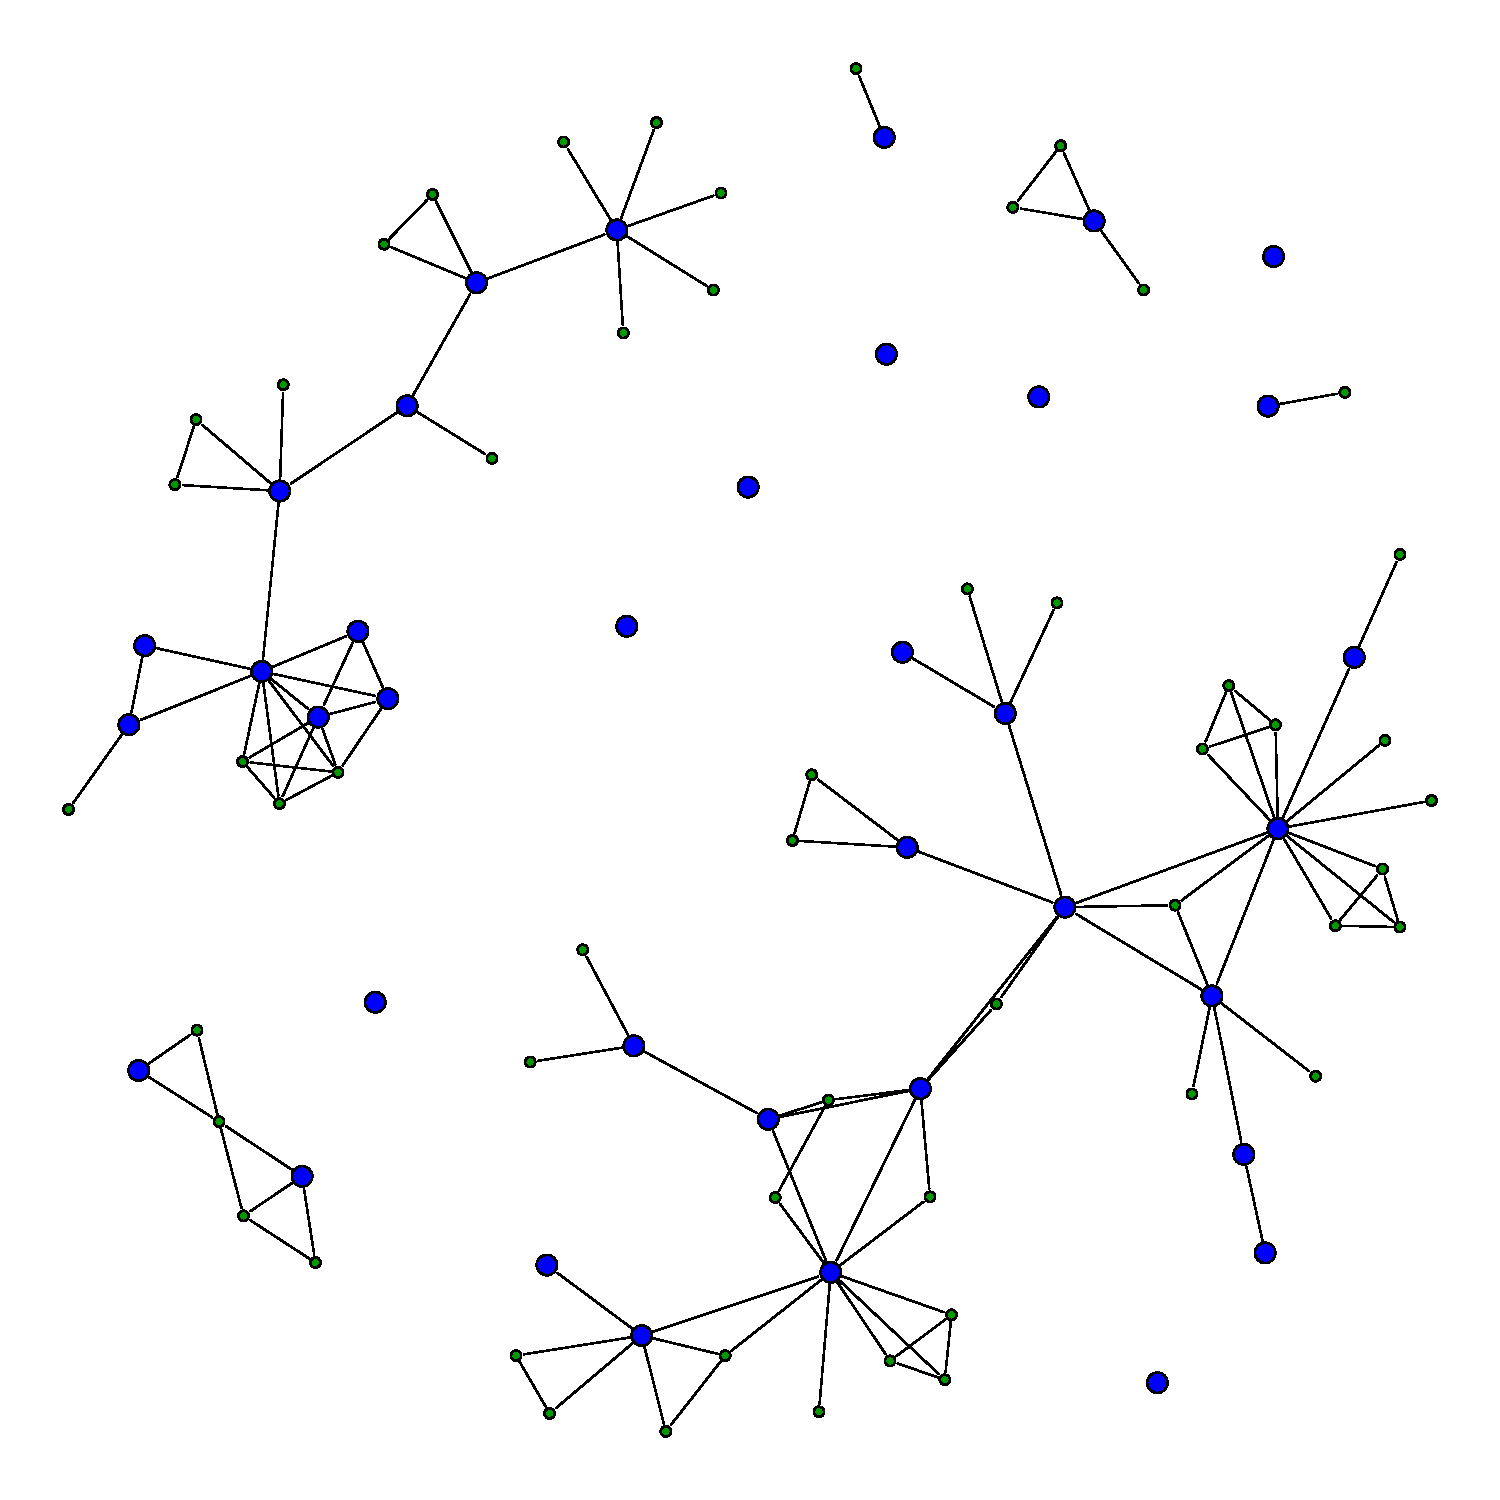
\includegraphics[width=.7\textwidth]{exemplo-grafo}
    \caption{Uma figura simples.\label{fig:subfigures:a}}
  \end{subfigure}
  % ATENÇÃO: Se você deixar uma linha em branco entre as subfiguras,
  % LaTeX vai considerar que cada uma delas pertence a um "parágrafo"
  % diferente e, portanto, vai colocá-las em linhas separadas ao invés
  % de lado a lado.
  \begin{subfigure}{0.4\textwidth}
    \centering
    \begin{turn}{90}
      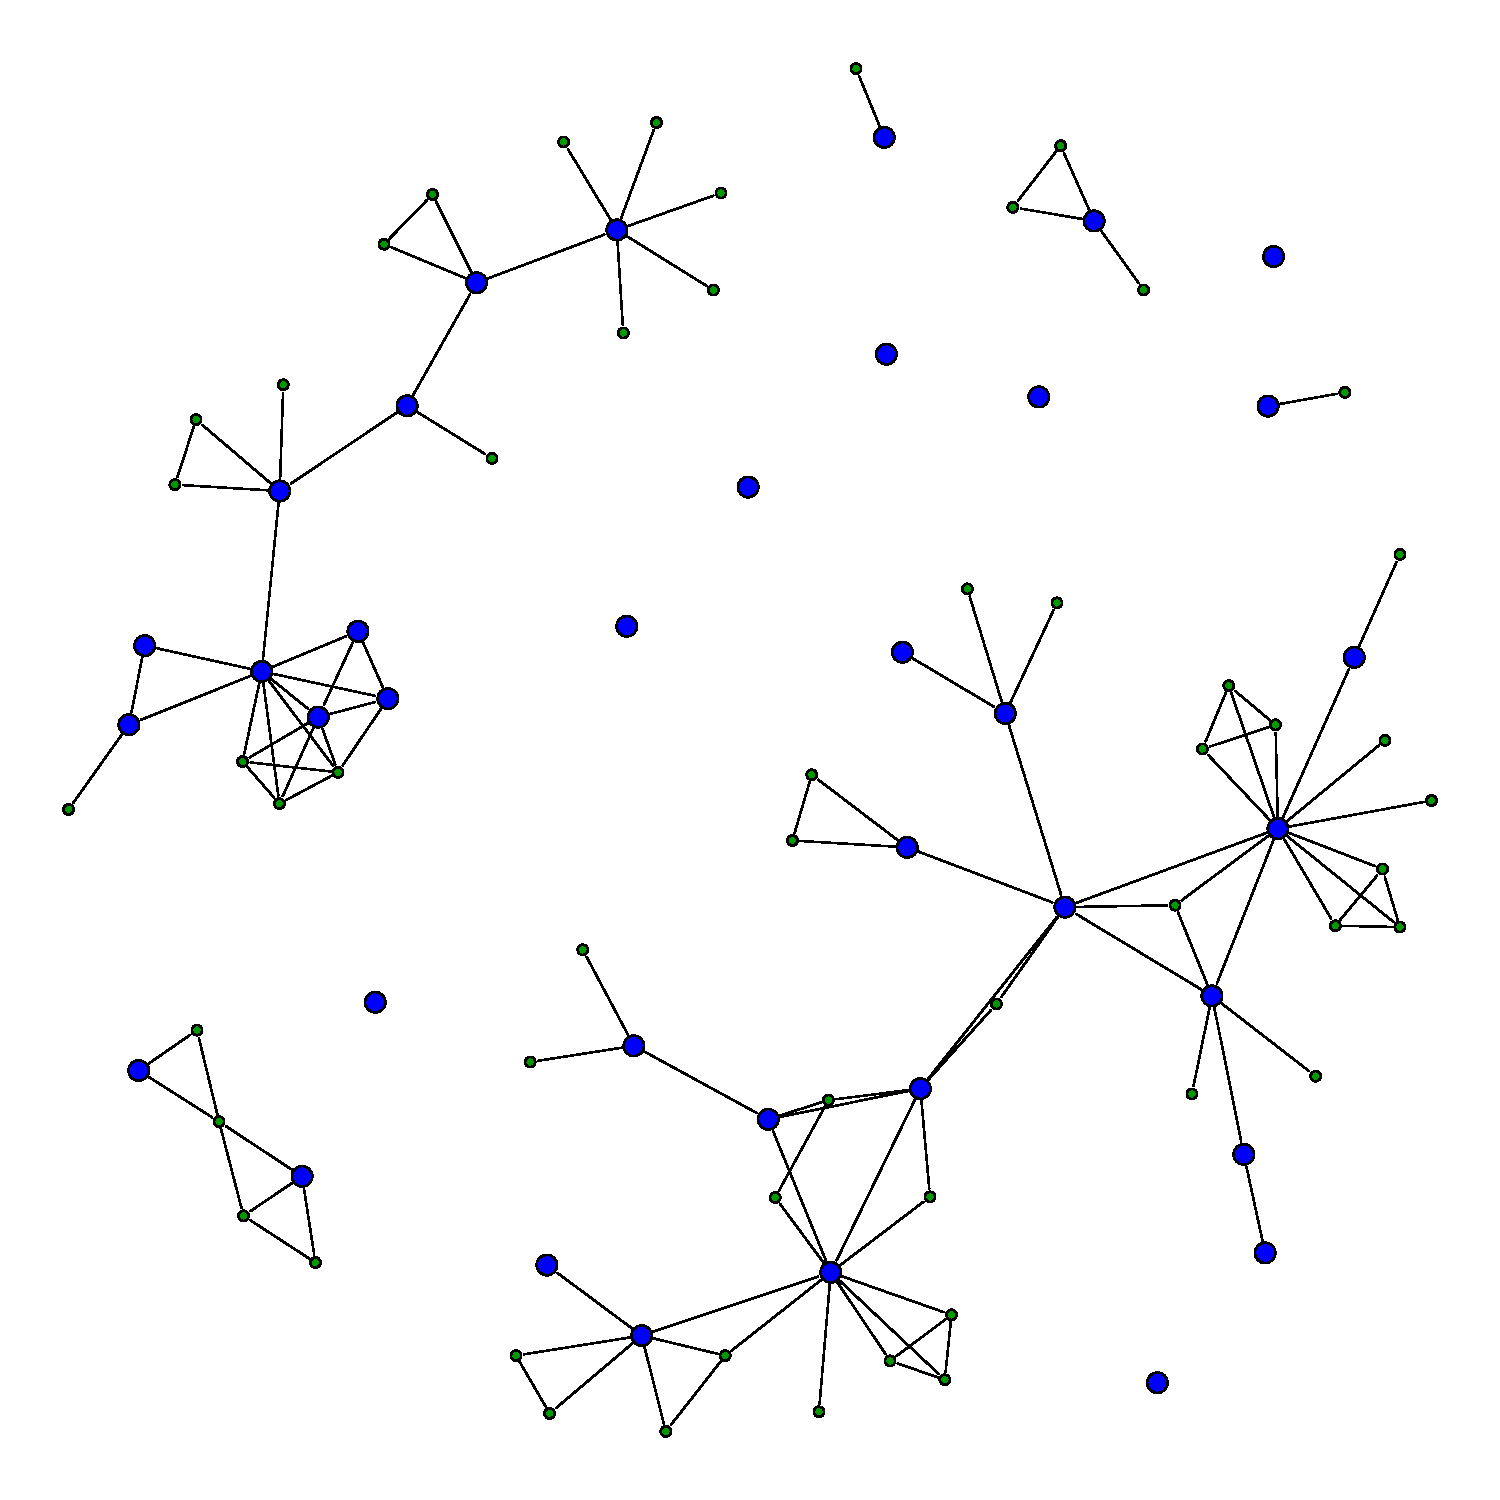
\includegraphics[width=.7\textwidth]{exemplo-grafo}
    \end{turn}
    \caption{O mesmo exemplo, girado.\label{fig:subfigures:b}}
  \end{subfigure}

  \caption{Exemplo de subfiguras.\label{fig:subfigures}}
\end{figure}

Uma ``figura'', na verdade, pode ser qualquer tipo de conteúdo ilustrativo
(um exemplo interessante é o cronograma mostrado na Figura~\ref{fig:gantt}) mas, com a
\textit{package} \textsf{float}, também é possível definir ambientes
específicos para cada tipo de conteúdo adicional (cada um com numeração
independente), como é o caso do Programa~\ref{prog:java}\index{Floats}. Há
mais informações e dicas sobre recursos específicos para inclusão de
código-fonte e pseudocódigo no Apêndice \ref{ap:pseudocode}\footnote{
Observe que o nome do Apêndice (``\ref{ap:pseudocode}'') foi impresso em
uma linha separada, o que não é muito bom visualmente. Para evitar que isso
aconteça (não só no final do parágrafo, mas em qualquer quebra de linha),
faça o que já foi discutido na Seção~\ref{orphanchar} sobre símbolos
matemáticos: utilize um espaço não-separável para fazer referências a
figuras, tabelas, seções etc.: ``\textsf{\dots no
Apêndice\textasciitilde\textbackslash{}ref\{ap:pseudocode\}}''.}.

%%%%%%% Cronograma %%%%%%%

\begin{figure}
  \centering

  \begin{ganttchart}{2017-11}{2018-5}
    \gantttitlecalendar{year,month=shortname} \ganttnewline

    \ganttgroup[progress=45]{Experimento}{2017-11}{2018-2} \ganttnewline
    \ganttbar[progress=100]{
      Preparação\ganttalignnewline
      (compra de insumos)
      }{2017-11}{2017-12} \ganttnewline
    \ganttbar[progress=30]{Execução}{2017-12}{2018-1} \ganttnewline
    \ganttbar[progress=0]{Análise}{2017-12}{2018-2} \ganttnewline

    \ganttgroup[progress=0]{Artigo}{2018-1}{2018-4} \ganttnewline
    \ganttbar[progress=0]{Escrita}{2018-1}{2018-3} \ganttnewline
    \ganttbar[progress=0]{Revisão}{2018-3}{2018-4} \ganttnewline

    \ganttmilestone{Submissão}{2018-4}
  \end{ganttchart}

  \caption{Exemplo de cronograma.\label{fig:gantt}}
\end{figure}

%%%%%%%% Código fonte %%%%%%%%

% Foi utilizado o pacote listings para formatar o código fonte.
% Veja os parâmetros de configuração no arquivo source-code.tex.
\begin{program}
  \index{Java}
  \centering

\begin{lstlisting}[language=Java, style=wider]
  for (i = 0; i < 20; i++)
  {
      // Comentário
      System.out.println("Mensagem...");
  }
\end{lstlisting}

  \caption{Exemplo de laço em Java.\label{prog:java}}
\end{program}

%%%%%

\LaTeX{} pode importar gráficos gerados por \texttt{matplotlib} e por
\texttt{gnuplot} como qualquer outra imagem, mas nesse caso a fonte
usada nesses gráficos provavelmente será diferente do corpo do texto.
Conforme mencionado na Seção~\ref{sec:graficos}, há mecanismos para
resolver esse problema\footnote{Você pode se interessar também pela
package \texttt{gnuplottex}.}, como pode ser visto na
Figura~\ref{fig:graficos}.

\begin{figure}
  \centering
  \begin{subfigure}{.65\textwidth}
    \input{figuras/gnuplot.tkz}
    \caption{\texttt{gnuplot}.\label{fig:gnuplot}}
  \end{subfigure}
  \begin{subfigure}{.3\textwidth}
    %% Creator: Matplotlib, PGF backend
%%
%% To include the figure in your LaTeX document, write
%%   \input{<filename>.pgf}
%%
%% Make sure the required packages are loaded in your preamble
%%   \usepackage{pgf}
%%
%% Figures using additional raster images can only be included by \input if
%% they are in the same directory as the main LaTeX file. For loading figures
%% from other directories you can use the `import` package
%%   \usepackage{import}
%% and then include the figures with
%%   \import{<path to file>}{<filename>.pgf}
%%
%% Matplotlib used the following preamble
%%   \usepackage{fontspec}
%%   \setmainfont{DejaVu Serif}
%%   \setsansfont{DejaVu Sans}
%%   \setmonofont{DejaVu Sans Mono}
%%
\begingroup%
\makeatletter%
\begin{pgfpicture}%
\pgfpathrectangle{\pgfpointorigin}{\pgfqpoint{1.500000in}{2.500000in}}%
\pgfusepath{use as bounding box, clip}%
\begin{pgfscope}%
\pgfsetbuttcap%
\pgfsetmiterjoin%
\definecolor{currentfill}{rgb}{1.000000,1.000000,1.000000}%
\pgfsetfillcolor{currentfill}%
\pgfsetlinewidth{0.000000pt}%
\definecolor{currentstroke}{rgb}{1.000000,1.000000,1.000000}%
\pgfsetstrokecolor{currentstroke}%
\pgfsetdash{}{0pt}%
\pgfpathmoveto{\pgfqpoint{0.000000in}{0.000000in}}%
\pgfpathlineto{\pgfqpoint{1.500000in}{0.000000in}}%
\pgfpathlineto{\pgfqpoint{1.500000in}{2.500000in}}%
\pgfpathlineto{\pgfqpoint{0.000000in}{2.500000in}}%
\pgfpathclose%
\pgfusepath{fill}%
\end{pgfscope}%
\begin{pgfscope}%
\pgfsetbuttcap%
\pgfsetmiterjoin%
\definecolor{currentfill}{rgb}{1.000000,1.000000,1.000000}%
\pgfsetfillcolor{currentfill}%
\pgfsetlinewidth{0.000000pt}%
\definecolor{currentstroke}{rgb}{0.000000,0.000000,0.000000}%
\pgfsetstrokecolor{currentstroke}%
\pgfsetstrokeopacity{0.000000}%
\pgfsetdash{}{0pt}%
\pgfpathmoveto{\pgfqpoint{0.385278in}{0.425278in}}%
\pgfpathlineto{\pgfqpoint{1.452500in}{0.425278in}}%
\pgfpathlineto{\pgfqpoint{1.452500in}{2.437500in}}%
\pgfpathlineto{\pgfqpoint{0.385278in}{2.437500in}}%
\pgfpathclose%
\pgfusepath{fill}%
\end{pgfscope}%
\begin{pgfscope}%
\pgfpathrectangle{\pgfqpoint{0.385278in}{0.425278in}}{\pgfqpoint{1.067222in}{2.012222in}} %
\pgfusepath{clip}%
\pgfsetbuttcap%
\pgfsetmiterjoin%
\definecolor{currentfill}{rgb}{0.121569,0.466667,0.705882}%
\pgfsetfillcolor{currentfill}%
\pgfsetlinewidth{0.000000pt}%
\definecolor{currentstroke}{rgb}{0.000000,0.000000,0.000000}%
\pgfsetstrokecolor{currentstroke}%
\pgfsetstrokeopacity{0.000000}%
\pgfsetdash{}{0pt}%
\pgfpathmoveto{\pgfqpoint{0.385278in}{0.425278in}}%
\pgfpathlineto{\pgfqpoint{0.690198in}{0.425278in}}%
\pgfpathlineto{\pgfqpoint{0.690198in}{1.096019in}}%
\pgfpathlineto{\pgfqpoint{0.385278in}{1.096019in}}%
\pgfpathclose%
\pgfusepath{fill}%
\end{pgfscope}%
\begin{pgfscope}%
\pgfpathrectangle{\pgfqpoint{0.385278in}{0.425278in}}{\pgfqpoint{1.067222in}{2.012222in}} %
\pgfusepath{clip}%
\pgfsetbuttcap%
\pgfsetmiterjoin%
\definecolor{currentfill}{rgb}{0.121569,0.466667,0.705882}%
\pgfsetfillcolor{currentfill}%
\pgfsetlinewidth{0.000000pt}%
\definecolor{currentstroke}{rgb}{0.000000,0.000000,0.000000}%
\pgfsetstrokecolor{currentstroke}%
\pgfsetstrokeopacity{0.000000}%
\pgfsetdash{}{0pt}%
\pgfpathmoveto{\pgfqpoint{0.766429in}{0.425278in}}%
\pgfpathlineto{\pgfqpoint{1.071349in}{0.425278in}}%
\pgfpathlineto{\pgfqpoint{1.071349in}{2.437500in}}%
\pgfpathlineto{\pgfqpoint{0.766429in}{2.437500in}}%
\pgfpathclose%
\pgfusepath{fill}%
\end{pgfscope}%
\begin{pgfscope}%
\pgfpathrectangle{\pgfqpoint{0.385278in}{0.425278in}}{\pgfqpoint{1.067222in}{2.012222in}} %
\pgfusepath{clip}%
\pgfsetbuttcap%
\pgfsetmiterjoin%
\definecolor{currentfill}{rgb}{0.121569,0.466667,0.705882}%
\pgfsetfillcolor{currentfill}%
\pgfsetlinewidth{0.000000pt}%
\definecolor{currentstroke}{rgb}{0.000000,0.000000,0.000000}%
\pgfsetstrokecolor{currentstroke}%
\pgfsetstrokeopacity{0.000000}%
\pgfsetdash{}{0pt}%
\pgfpathmoveto{\pgfqpoint{1.147579in}{0.425278in}}%
\pgfpathlineto{\pgfqpoint{1.452500in}{0.425278in}}%
\pgfpathlineto{\pgfqpoint{1.452500in}{1.766759in}}%
\pgfpathlineto{\pgfqpoint{1.147579in}{1.766759in}}%
\pgfpathclose%
\pgfusepath{fill}%
\end{pgfscope}%
\begin{pgfscope}%
\pgfsetbuttcap%
\pgfsetroundjoin%
\definecolor{currentfill}{rgb}{0.000000,0.000000,0.000000}%
\pgfsetfillcolor{currentfill}%
\pgfsetlinewidth{0.803000pt}%
\definecolor{currentstroke}{rgb}{0.000000,0.000000,0.000000}%
\pgfsetstrokecolor{currentstroke}%
\pgfsetdash{}{0pt}%
\pgfsys@defobject{currentmarker}{\pgfqpoint{0.000000in}{-0.048611in}}{\pgfqpoint{0.000000in}{0.000000in}}{%
\pgfpathmoveto{\pgfqpoint{0.000000in}{0.000000in}}%
\pgfpathlineto{\pgfqpoint{0.000000in}{-0.048611in}}%
\pgfusepath{stroke,fill}%
}%
\begin{pgfscope}%
\pgfsys@transformshift{0.537738in}{0.425278in}%
\pgfsys@useobject{currentmarker}{}%
\end{pgfscope}%
\end{pgfscope}%
\begin{pgfscope}%
\pgftext[x=0.537738in,y=0.328056in,,top]{\rmfamily\fontsize{9.000000}{10.800000}\selectfont SP}%
\end{pgfscope}%
\begin{pgfscope}%
\pgfsetbuttcap%
\pgfsetroundjoin%
\definecolor{currentfill}{rgb}{0.000000,0.000000,0.000000}%
\pgfsetfillcolor{currentfill}%
\pgfsetlinewidth{0.803000pt}%
\definecolor{currentstroke}{rgb}{0.000000,0.000000,0.000000}%
\pgfsetstrokecolor{currentstroke}%
\pgfsetdash{}{0pt}%
\pgfsys@defobject{currentmarker}{\pgfqpoint{0.000000in}{-0.048611in}}{\pgfqpoint{0.000000in}{0.000000in}}{%
\pgfpathmoveto{\pgfqpoint{0.000000in}{0.000000in}}%
\pgfpathlineto{\pgfqpoint{0.000000in}{-0.048611in}}%
\pgfusepath{stroke,fill}%
}%
\begin{pgfscope}%
\pgfsys@transformshift{0.918889in}{0.425278in}%
\pgfsys@useobject{currentmarker}{}%
\end{pgfscope}%
\end{pgfscope}%
\begin{pgfscope}%
\pgftext[x=0.918889in,y=0.328056in,,top]{\rmfamily\fontsize{9.000000}{10.800000}\selectfont RJ}%
\end{pgfscope}%
\begin{pgfscope}%
\pgfsetbuttcap%
\pgfsetroundjoin%
\definecolor{currentfill}{rgb}{0.000000,0.000000,0.000000}%
\pgfsetfillcolor{currentfill}%
\pgfsetlinewidth{0.803000pt}%
\definecolor{currentstroke}{rgb}{0.000000,0.000000,0.000000}%
\pgfsetstrokecolor{currentstroke}%
\pgfsetdash{}{0pt}%
\pgfsys@defobject{currentmarker}{\pgfqpoint{0.000000in}{-0.048611in}}{\pgfqpoint{0.000000in}{0.000000in}}{%
\pgfpathmoveto{\pgfqpoint{0.000000in}{0.000000in}}%
\pgfpathlineto{\pgfqpoint{0.000000in}{-0.048611in}}%
\pgfusepath{stroke,fill}%
}%
\begin{pgfscope}%
\pgfsys@transformshift{1.300040in}{0.425278in}%
\pgfsys@useobject{currentmarker}{}%
\end{pgfscope}%
\end{pgfscope}%
\begin{pgfscope}%
\pgftext[x=1.300040in,y=0.328056in,,top]{\rmfamily\fontsize{9.000000}{10.800000}\selectfont MG}%
\end{pgfscope}%
\begin{pgfscope}%
\pgftext[x=0.918889in,y=0.151528in,,top]{\rmfamily\fontsize{9.000000}{10.800000}\selectfont \textit{Estado}}%
\end{pgfscope}%
\begin{pgfscope}%
\pgfsetbuttcap%
\pgfsetroundjoin%
\definecolor{currentfill}{rgb}{0.000000,0.000000,0.000000}%
\pgfsetfillcolor{currentfill}%
\pgfsetlinewidth{0.803000pt}%
\definecolor{currentstroke}{rgb}{0.000000,0.000000,0.000000}%
\pgfsetstrokecolor{currentstroke}%
\pgfsetdash{}{0pt}%
\pgfsys@defobject{currentmarker}{\pgfqpoint{-0.048611in}{0.000000in}}{\pgfqpoint{0.000000in}{0.000000in}}{%
\pgfpathmoveto{\pgfqpoint{0.000000in}{0.000000in}}%
\pgfpathlineto{\pgfqpoint{-0.048611in}{0.000000in}}%
\pgfusepath{stroke,fill}%
}%
\begin{pgfscope}%
\pgfsys@transformshift{0.385278in}{0.425278in}%
\pgfsys@useobject{currentmarker}{}%
\end{pgfscope}%
\end{pgfscope}%
\begin{pgfscope}%
\pgftext[x=0.208527in,y=0.377792in,left,base]{\rmfamily\fontsize{9.000000}{10.800000}\selectfont 0}%
\end{pgfscope}%
\begin{pgfscope}%
\pgfsetbuttcap%
\pgfsetroundjoin%
\definecolor{currentfill}{rgb}{0.000000,0.000000,0.000000}%
\pgfsetfillcolor{currentfill}%
\pgfsetlinewidth{0.803000pt}%
\definecolor{currentstroke}{rgb}{0.000000,0.000000,0.000000}%
\pgfsetstrokecolor{currentstroke}%
\pgfsetdash{}{0pt}%
\pgfsys@defobject{currentmarker}{\pgfqpoint{-0.048611in}{0.000000in}}{\pgfqpoint{0.000000in}{0.000000in}}{%
\pgfpathmoveto{\pgfqpoint{0.000000in}{0.000000in}}%
\pgfpathlineto{\pgfqpoint{-0.048611in}{0.000000in}}%
\pgfusepath{stroke,fill}%
}%
\begin{pgfscope}%
\pgfsys@transformshift{0.385278in}{0.760648in}%
\pgfsys@useobject{currentmarker}{}%
\end{pgfscope}%
\end{pgfscope}%
\begin{pgfscope}%
\pgftext[x=0.208527in,y=0.713163in,left,base]{\rmfamily\fontsize{9.000000}{10.800000}\selectfont 1}%
\end{pgfscope}%
\begin{pgfscope}%
\pgfsetbuttcap%
\pgfsetroundjoin%
\definecolor{currentfill}{rgb}{0.000000,0.000000,0.000000}%
\pgfsetfillcolor{currentfill}%
\pgfsetlinewidth{0.803000pt}%
\definecolor{currentstroke}{rgb}{0.000000,0.000000,0.000000}%
\pgfsetstrokecolor{currentstroke}%
\pgfsetdash{}{0pt}%
\pgfsys@defobject{currentmarker}{\pgfqpoint{-0.048611in}{0.000000in}}{\pgfqpoint{0.000000in}{0.000000in}}{%
\pgfpathmoveto{\pgfqpoint{0.000000in}{0.000000in}}%
\pgfpathlineto{\pgfqpoint{-0.048611in}{0.000000in}}%
\pgfusepath{stroke,fill}%
}%
\begin{pgfscope}%
\pgfsys@transformshift{0.385278in}{1.096019in}%
\pgfsys@useobject{currentmarker}{}%
\end{pgfscope}%
\end{pgfscope}%
\begin{pgfscope}%
\pgftext[x=0.208527in,y=1.048533in,left,base]{\rmfamily\fontsize{9.000000}{10.800000}\selectfont 2}%
\end{pgfscope}%
\begin{pgfscope}%
\pgfsetbuttcap%
\pgfsetroundjoin%
\definecolor{currentfill}{rgb}{0.000000,0.000000,0.000000}%
\pgfsetfillcolor{currentfill}%
\pgfsetlinewidth{0.803000pt}%
\definecolor{currentstroke}{rgb}{0.000000,0.000000,0.000000}%
\pgfsetstrokecolor{currentstroke}%
\pgfsetdash{}{0pt}%
\pgfsys@defobject{currentmarker}{\pgfqpoint{-0.048611in}{0.000000in}}{\pgfqpoint{0.000000in}{0.000000in}}{%
\pgfpathmoveto{\pgfqpoint{0.000000in}{0.000000in}}%
\pgfpathlineto{\pgfqpoint{-0.048611in}{0.000000in}}%
\pgfusepath{stroke,fill}%
}%
\begin{pgfscope}%
\pgfsys@transformshift{0.385278in}{1.431389in}%
\pgfsys@useobject{currentmarker}{}%
\end{pgfscope}%
\end{pgfscope}%
\begin{pgfscope}%
\pgftext[x=0.208527in,y=1.383904in,left,base]{\rmfamily\fontsize{9.000000}{10.800000}\selectfont 3}%
\end{pgfscope}%
\begin{pgfscope}%
\pgfsetbuttcap%
\pgfsetroundjoin%
\definecolor{currentfill}{rgb}{0.000000,0.000000,0.000000}%
\pgfsetfillcolor{currentfill}%
\pgfsetlinewidth{0.803000pt}%
\definecolor{currentstroke}{rgb}{0.000000,0.000000,0.000000}%
\pgfsetstrokecolor{currentstroke}%
\pgfsetdash{}{0pt}%
\pgfsys@defobject{currentmarker}{\pgfqpoint{-0.048611in}{0.000000in}}{\pgfqpoint{0.000000in}{0.000000in}}{%
\pgfpathmoveto{\pgfqpoint{0.000000in}{0.000000in}}%
\pgfpathlineto{\pgfqpoint{-0.048611in}{0.000000in}}%
\pgfusepath{stroke,fill}%
}%
\begin{pgfscope}%
\pgfsys@transformshift{0.385278in}{1.766759in}%
\pgfsys@useobject{currentmarker}{}%
\end{pgfscope}%
\end{pgfscope}%
\begin{pgfscope}%
\pgftext[x=0.208527in,y=1.719274in,left,base]{\rmfamily\fontsize{9.000000}{10.800000}\selectfont 4}%
\end{pgfscope}%
\begin{pgfscope}%
\pgfsetbuttcap%
\pgfsetroundjoin%
\definecolor{currentfill}{rgb}{0.000000,0.000000,0.000000}%
\pgfsetfillcolor{currentfill}%
\pgfsetlinewidth{0.803000pt}%
\definecolor{currentstroke}{rgb}{0.000000,0.000000,0.000000}%
\pgfsetstrokecolor{currentstroke}%
\pgfsetdash{}{0pt}%
\pgfsys@defobject{currentmarker}{\pgfqpoint{-0.048611in}{0.000000in}}{\pgfqpoint{0.000000in}{0.000000in}}{%
\pgfpathmoveto{\pgfqpoint{0.000000in}{0.000000in}}%
\pgfpathlineto{\pgfqpoint{-0.048611in}{0.000000in}}%
\pgfusepath{stroke,fill}%
}%
\begin{pgfscope}%
\pgfsys@transformshift{0.385278in}{2.102130in}%
\pgfsys@useobject{currentmarker}{}%
\end{pgfscope}%
\end{pgfscope}%
\begin{pgfscope}%
\pgftext[x=0.208527in,y=2.054644in,left,base]{\rmfamily\fontsize{9.000000}{10.800000}\selectfont 5}%
\end{pgfscope}%
\begin{pgfscope}%
\pgfsetbuttcap%
\pgfsetroundjoin%
\definecolor{currentfill}{rgb}{0.000000,0.000000,0.000000}%
\pgfsetfillcolor{currentfill}%
\pgfsetlinewidth{0.803000pt}%
\definecolor{currentstroke}{rgb}{0.000000,0.000000,0.000000}%
\pgfsetstrokecolor{currentstroke}%
\pgfsetdash{}{0pt}%
\pgfsys@defobject{currentmarker}{\pgfqpoint{-0.048611in}{0.000000in}}{\pgfqpoint{0.000000in}{0.000000in}}{%
\pgfpathmoveto{\pgfqpoint{0.000000in}{0.000000in}}%
\pgfpathlineto{\pgfqpoint{-0.048611in}{0.000000in}}%
\pgfusepath{stroke,fill}%
}%
\begin{pgfscope}%
\pgfsys@transformshift{0.385278in}{2.437500in}%
\pgfsys@useobject{currentmarker}{}%
\end{pgfscope}%
\end{pgfscope}%
\begin{pgfscope}%
\pgftext[x=0.208527in,y=2.390015in,left,base]{\rmfamily\fontsize{9.000000}{10.800000}\selectfont 6}%
\end{pgfscope}%
\begin{pgfscope}%
\pgftext[x=0.152971in,y=1.431389in,,bottom,rotate=90.000000]{\rmfamily\fontsize{9.000000}{10.800000}\selectfont \(\displaystyle \mu\)}%
\end{pgfscope}%
\begin{pgfscope}%
\pgfsetrectcap%
\pgfsetmiterjoin%
\pgfsetlinewidth{0.803000pt}%
\definecolor{currentstroke}{rgb}{0.000000,0.000000,0.000000}%
\pgfsetstrokecolor{currentstroke}%
\pgfsetdash{}{0pt}%
\pgfpathmoveto{\pgfqpoint{0.385278in}{0.425278in}}%
\pgfpathlineto{\pgfqpoint{0.385278in}{2.437500in}}%
\pgfusepath{stroke}%
\end{pgfscope}%
\begin{pgfscope}%
\pgfsetrectcap%
\pgfsetmiterjoin%
\pgfsetlinewidth{0.803000pt}%
\definecolor{currentstroke}{rgb}{0.000000,0.000000,0.000000}%
\pgfsetstrokecolor{currentstroke}%
\pgfsetdash{}{0pt}%
\pgfpathmoveto{\pgfqpoint{1.452500in}{0.425278in}}%
\pgfpathlineto{\pgfqpoint{1.452500in}{2.437500in}}%
\pgfusepath{stroke}%
\end{pgfscope}%
\begin{pgfscope}%
\pgfsetrectcap%
\pgfsetmiterjoin%
\pgfsetlinewidth{0.803000pt}%
\definecolor{currentstroke}{rgb}{0.000000,0.000000,0.000000}%
\pgfsetstrokecolor{currentstroke}%
\pgfsetdash{}{0pt}%
\pgfpathmoveto{\pgfqpoint{0.385278in}{0.425278in}}%
\pgfpathlineto{\pgfqpoint{1.452500in}{0.425278in}}%
\pgfusepath{stroke}%
\end{pgfscope}%
\begin{pgfscope}%
\pgfsetrectcap%
\pgfsetmiterjoin%
\pgfsetlinewidth{0.803000pt}%
\definecolor{currentstroke}{rgb}{0.000000,0.000000,0.000000}%
\pgfsetstrokecolor{currentstroke}%
\pgfsetdash{}{0pt}%
\pgfpathmoveto{\pgfqpoint{0.385278in}{2.437500in}}%
\pgfpathlineto{\pgfqpoint{1.452500in}{2.437500in}}%
\pgfusepath{stroke}%
\end{pgfscope}%
\end{pgfpicture}%
\makeatother%
\endgroup%

    \caption{\texttt{matplotlib}.\label{fig:matplotlib}}
  \end{subfigure}
	\caption{Exemplos de gráficos gerados externamente}\label{fig:graficos}
\end{figure}

Finalmente, talvez você precise organizar a apresentação da informação na forma de
tabelas\index{Floats}\footnote{Para defini-las com \LaTeX{}, pode valer a pena usar o
sítio \url{www.tablesgenerator.com}.}; Um exemplo simples é a Tabela~\ref{tab:amino_acidos}.

%%%%%%%% Tabelas lado-a-lado %%%%%%%%

\begin{table}
\centering

  \hspace*{\fill}
  \begin{subtable}[b]{0.42\textwidth}
    % \rowcolors é definida pela package xcolor;
    % veja também os recursos da package colortbl
    \rowcolors{2}{lightgray!70}{white}
    \centering
    \begin{tabular}{ccl}
      \toprule
      Código      & Abreviatura  & \makecell{Nome\\completo} \\
      \midrule
      \texttt{A}  & Ala          & Alanina \\
      \texttt{C}  & Cys          & Cisteína \\
      ...         & ...          & ... \\
      \texttt{W}  & Trp          & Triptofano \\
      \texttt{Y}  & Tyr          & Tirosina \\
      \bottomrule
    \end{tabular}
    \caption{Com linhas de cores alternadas.}
  \end{subtable}
  % Como mencionado mais acima, não deixe linhas em branco aqui
  \hspace*{\fill}\hspace*{\fill}\hspace*{\fill}
  \begin{subtable}[b]{0.37\textwidth}
    \centering
    \begin{tabular}{ccl}
      \rothead{Código} & \rothead{Abreviatura} & \rothead{Nome\\completo} \\
      \midrule
      \texttt{A}       & Ala                   & Alanina \\
      \texttt{C}       & Cys                   & Cisteína \\
      ...              & ...                   & ... \\
      \texttt{W}       & Trp                   & Triptofano \\
      \texttt{Y}       & Tyr                   & Tirosina \\
      \bottomrule
    \end{tabular}
    \caption{Com cabeçalhos girados.}
  \end{subtable}
  \hspace*{\fill}

  \caption{Exemplos de tabelas (códigos, abreviaturas e nomes dos aminoácidos).\label{tab:amino_acidos}}
\end{table}

Se a tabela tem muitas linhas e, portanto, não cabe em uma única página, é
possível fazê-la continuar ao longo de várias páginas com a \textit{package}
\textsf{longtable}, como é o caso da Tabela~\ref{tab:numeros}. Nesse caso,
a tabela não é um \textit{float} e, portanto, ela aparece de acordo com a
sequência normal do texto. Se, além de muito longa, a tabela for também
muito larga, você pode usar o comando \textsf{landscape} (da
\textit{package} \textsf{pdflscape}) em conjunto com \textsf{longtable}
para imprimi-la em modo paisagem ao longo de várias páginas. A
Tabela~\ref{tab:numeros} tem essa configuração comentada; experimente
des-comentar as linhas correspondentes\footnote{Observe que, nesse caso,
vai sempre haver uma quebra de página no texto para fazer a tabela
começar em uma página em modo paisagem.}.

%%%%%%%% Tabela longa em várias páginas %%%%%%%%

%%%% É possível fazer esta mesma tabela em modo paisagem des-comentando
%%%% esta linha e a correspondente no final da tabela
%\begin{landscape}
\begin{longtable}[c]{|c|c|c|c|c|c|c|c|c|c|c|c|c|}

%%%%%%%%%%%%
% O cabeçalho da tabela na primeira página em que ela aparece.

\hline
% Como a tabela pode se estender por várias páginas, precisamos tomar
% cuidado especial com \caption e \label: se esses comandos forem
% executados mais de uma vez, a lista de tabelas e as referências à
% tabela ficarão incorretas. Há diversas soluções, mas a mais simples
% é usar "\caption[]", que não coloca a tabela na lista de tabelas, e
% incluí-la manualmente na lista apenas uma vez aqui junto com o \label.
\captionlistentry{Exemplo de tabela com valores numéricos.}\label{tab:numeros}

\emph{Lim.} &
\multicolumn{3}{c|}{MGWT} &
\multicolumn{3}{c|}{AMI} &
\multicolumn{3}{c|}{\emph{Spectrum} de Fourier} &
\multicolumn{3}{c|}{Caract. espectrais} \\

\cline{2-4} \cline{5-7} \cline{8-10} \cline{11-13} &
\emph{Sn} & \emph{Sp} & \emph{AC} &
\emph{Sn} & \emph{Sp} & \emph{AC} &
\emph{Sn} & \emph{Sp} & \emph{AC} &
\emph{Sn} & \emph{Sp} & \emph{AC} \\

\hline \hline

\endfirsthead % Final do cabeçalho que aparece na primeira página

%%%%%%%%%%%%
% O cabeçalho da tabela em todas as páginas em que ela aparece
% exceto a primeira; aqui, igual ao anterior

\hline

\emph{Lim.} &
\multicolumn{3}{c|}{MGWT} &
\multicolumn{3}{c|}{AMI} &
\multicolumn{3}{c|}{\emph{Spectrum} de Fourier} &
\multicolumn{3}{c|}{Caract. espectrais} \\

\cline{2-4} \cline{5-7} \cline{8-10} \cline{11-13} &
\emph{Sn} & \emph{Sp} & \emph{AC} &
\emph{Sn} & \emph{Sp} & \emph{AC} &
\emph{Sn} & \emph{Sp} & \emph{AC} &
\emph{Sn} & \emph{Sp} & \emph{AC} \\

\hline \hline

\endhead % Final do cabeçalho das páginas seguintes à primeira

%%%%%%%%%%%%
% O rodapé da tabela em todas as páginas em que ela aparece
% exceto a última

\hline

\multicolumn{13}{|r|}{\textit{continua}\enspace$\longrightarrow$}\\

\hline

% Como usamos \captionlistentry mais acima, usamos "[]" aqui.
\caption[]{Exemplo de tabela com valores numéricos.}

\endfoot % Final do rodapé que aparece em todas as páginas exceto a última

%%%%%%%%%%%%
% O rodapé da tabela na última página em que ela aparece

\hline

% Como usamos \captionlistentry mais acima, usamos "[]" aqui.
\caption[]{Exemplo de tabela com valores numéricos.}

\endlastfoot % Final do rodapé da última página

%%%%%%%%%%%%
% O conteúdo da tabela de fato.

 1 & 1.00 & 0.16 & 0.08 & 1.00 & 0.16 & 0.08 & 1.00 & 0.16 & 0.08 & 1.00 & 0.16 & 0.08 \\
 2 & 1.00 & 0.16 & 0.09 & 1.00 & 0.16 & 0.09 & 1.00 & 0.16 & 0.09 & 1.00 & 0.16 & 0.09 \\
 3 & 1.00 & 0.16 & 0.10 & 1.00 & 0.16 & 0.10 & 1.00 & 0.16 & 0.10 & 1.00 & 0.16 & 0.10 \\
 4 & 1.00 & 0.16 & 0.10 & 1.00 & 0.16 & 0.10 & 1.00 & 0.16 & 0.10 & 1.00 & 0.16 & 0.10 \\
 5 & 1.00 & 0.16 & 0.11 & 1.00 & 0.16 & 0.11 & 1.00 & 0.16 & 0.11 & 1.00 & 0.16 & 0.11 \\
 6 & 1.00 & 0.16 & 0.12 & 1.00 & 0.16 & 0.12 & 1.00 & 0.16 & 0.12 & 1.00 & 0.16 & 0.12 \\
 7 & 1.00 & 0.17 & 0.12 & 1.00 & 0.17 & 0.12 & 1.00 & 0.17 & 0.12 & 1.00 & 0.17 & 0.13 \\
 8 & 1.00 & 0.17 & 0.13 & 1.00 & 0.17 & 0.13 & 1.00 & 0.17 & 0.13 & 1.00 & 0.17 & 0.13 \\
 9 & 1.00 & 0.17 & 0.14 & 1.00 & 0.17 & 0.14 & 1.00 & 0.17 & 0.14 & 1.00 & 0.17 & 0.14 \\
10 & 1.00 & 0.17 & 0.15 & 1.00 & 0.17 & 0.15 & 1.00 & 0.17 & 0.15 & 1.00 & 0.17 & 0.15 \\
11 & 1.00 & 0.17 & 0.15 & 1.00 & 0.17 & 0.15 & 1.00 & 0.17 & 0.15 & 1.00 & 0.17 & 0.15 \\
12 & 1.00 & 0.18 & 0.16 & 1.00 & 0.18 & 0.16 & 1.00 & 0.18 & 0.16 & 1.00 & 0.18 & 0.16 \\
13 & 1.00 & 0.18 & 0.17 & 1.00 & 0.18 & 0.17 & 1.00 & 0.18 & 0.17 & 1.00 & 0.18 & 0.17 \\
14 & 1.00 & 0.18 & 0.17 & 1.00 & 0.18 & 0.17 & 1.00 & 0.18 & 0.17 & 1.00 & 0.18 & 0.17 \\
% Como nesta página há uma nota de rodapé, a linha separadora da
% nota e o final da tabela ficam muito próximos; vamos forçar uma
% quebra de página uma linha antes para resolver isso.
\pagebreak
15 & 1.00 & 0.18 & 0.18 & 1.00 & 0.18 & 0.18 & 1.00 & 0.18 & 0.18 & 1.00 & 0.18 & 0.18 \\
16 & 1.00 & 0.18 & 0.19 & 1.00 & 0.18 & 0.19 & 1.00 & 0.18 & 0.19 & 1.00 & 0.18 & 0.19 \\
17 & 1.00 & 0.19 & 0.19 & 1.00 & 0.19 & 0.19 & 1.00 & 0.19 & 0.19 & 1.00 & 0.19 & 0.19 \\
18 & 1.00 & 0.19 & 0.20 & 1.00 & 0.19 & 0.20 & 1.00 & 0.19 & 0.20 & 1.00 & 0.19 & 0.20 \\
19 & 1.00 & 0.19 & 0.21 & 1.00 & 0.19 & 0.21 & 1.00 & 0.19 & 0.21 & 1.00 & 0.19 & 0.21 \\
20 & 1.00 & 0.19 & 0.22 & 1.00 & 0.19 & 0.22 & 1.00 & 0.19 & 0.22 & 1.00 & 0.19 & 0.22 \\
21 & 1.00 & 0.19 & 0.22 & 1.00 & 0.19 & 0.22 & 1.00 & 0.19 & 0.22 & 1.00 & 0.19 & 0.22 \\
22 & 1.00 & 0.19 & 0.22 & 1.00 & 0.19 & 0.22 & 1.00 & 0.19 & 0.22 & 1.00 & 0.19 & 0.22 \\
23 & 1.00 & 0.19 & 0.22 & 1.00 & 0.19 & 0.22 & 1.00 & 0.19 & 0.22 & 1.00 & 0.19 & 0.22 \\
24 & 1.00 & 0.19 & 0.22 & 1.00 & 0.19 & 0.22 & 1.00 & 0.19 & 0.22 & 1.00 & 0.19 & 0.22 \\
25 & 1.00 & 0.19 & 0.22 & 1.00 & 0.19 & 0.22 & 1.00 & 0.19 & 0.22 & 1.00 & 0.19 & 0.22 \\
26 & 1.00 & 0.19 & 0.22 & 1.00 & 0.19 & 0.22 & 1.00 & 0.19 & 0.22 & 1.00 & 0.19 & 0.22 \\
27 & 1.00 & 0.19 & 0.22 & 1.00 & 0.19 & 0.22 & 1.00 & 0.19 & 0.22 & 1.00 & 0.19 & 0.22 \\
28 & 1.00 & 0.19 & 0.22 & 1.00 & 0.19 & 0.22 & 1.00 & 0.19 & 0.22 & 1.00 & 0.19 & 0.22 \\
29 & 1.00 & 0.19 & 0.22 & 1.00 & 0.19 & 0.22 & 1.00 & 0.19 & 0.22 & 1.00 & 0.19 & 0.22 \\
30 & 1.00 & 0.19 & 0.22 & 1.00 & 0.19 & 0.22 & 1.00 & 0.19 & 0.22 & 1.00 & 0.19 & 0.22 \\
31 & 1.00 & 0.19 & 0.22 & 1.00 & 0.19 & 0.22 & 1.00 & 0.19 & 0.22 & 1.00 & 0.19 & 0.22 \\
32 & 1.00 & 0.19 & 0.22 & 1.00 & 0.19 & 0.22 & 1.00 & 0.19 & 0.22 & 1.00 & 0.19 & 0.22 \\
33 & 1.00 & 0.19 & 0.22 & 1.00 & 0.19 & 0.22 & 1.00 & 0.19 & 0.22 & 1.00 & 0.19 & 0.22 \\
34 & 1.00 & 0.19 & 0.22 & 1.00 & 0.19 & 0.22 & 1.00 & 0.19 & 0.22 & 1.00 & 0.19 & 0.22 \\
35 & 1.00 & 0.19 & 0.22 & 1.00 & 0.19 & 0.22 & 1.00 & 0.19 & 0.22 & 1.00 & 0.19 & 0.22 \\
36 & 1.00 & 0.19 & 0.22 & 1.00 & 0.19 & 0.22 & 1.00 & 0.19 & 0.22 & 1.00 & 0.19 & 0.22 \\
37 & 1.00 & 0.19 & 0.22 & 1.00 & 0.19 & 0.22 & 1.00 & 0.19 & 0.22 & 1.00 & 0.19 & 0.22 \\
38 & 1.00 & 0.19 & 0.22 & 1.00 & 0.19 & 0.22 & 1.00 & 0.19 & 0.22 & 1.00 & 0.19 & 0.22 \\
39 & 1.00 & 0.19 & 0.22 & 1.00 & 0.19 & 0.22 & 1.00 & 0.19 & 0.22 & 1.00 & 0.19 & 0.22 \\
40 & 1.00 & 0.19 & 0.22 & 1.00 & 0.19 & 0.22 & 1.00 & 0.19 & 0.22 & 1.00 & 0.19 & 0.22 \\
\end{longtable}
%\end{landscape}

Tabelas mais complexas são um tanto trabalhosas em \LaTeX{}; a
Tabela~\ref{tab:ficha} mostra como construir uma tabela em forma de ficha.
Além de complexa, ela é larga e, portanto, deve ser impressa em modo
paisagem. No entanto, usamos um outro mecanismo para girar a tabela: o
comando \textsf{sidewaystable} (da \textit{package} \textsf{rotating}).
Com esse mecanismo, ela continua sendo um \textit{float} (e, portanto,
não força quebras de página no meio do texto), mas sempre é impressa em
uma página separada.

Resumindo:

\begin{itemize}
  \item Se uma tabela cabe em uma página, defina-a como um \textit{float};
  \item se cabe em uma página mas é muito larga e precisa ser impressa em
        modo paisagem, use \textsf{sidewaystable} (que também é um \textit{float});
  \item se não cabe em uma página por ser muito longa, use \textsf{longtable};
  \item se não cabe em uma página por ser muito longa e precisa ser impressa
        em modo paisagem por ser muito larga, use \textsf{longtable} em
        conjunto com \textsf{landscape}.
\end{itemize}

%%%%%%%% Tabela em forma de ficha %%%%%%%%

% Aumenta o espaçamento entre as linhas da tabela (default: 0pt)
\setlength\extrarowheight{4pt}

% sidewaystable e comandos relacionados são definidos na package rotating
\begin{sidewaystable}
\centering

\begin{tabular}{|M{0.265}|M{0.073}|M{0.084}|M{0.073}|M{0.073}|M{0.08}|M{0.082}|M{0.067}|}
  \hline
    \textbf{Experimento número:} & \multicolumn{2}{c|}{1} & \multicolumn{4}{c|}{\textbf{Data:}} & jan 2017
  \tabularnewline \hline
    \textbf{Título:} & \multicolumn{7}{c|}{Medições iniciais}
  \tabularnewline \hline
    \textbf{Tipo de experimento:} & \multicolumn{7}{c|}{Levantamento quantitativo}
  \tabularnewline \hline \hline
    \textbf{Locais}          & São Paulo & Rio de Janeiro & Porto Alegre & Recife & Manaus & Brasília & Rio Branco
  \tabularnewline \thickhline
    \textbf{Valores obtidos} & 0.2       & 0.3            & 0.2          & 0.7    & 0.5    & 0.1      & 0.4
  \tabularnewline \hline
\end{tabular}

\caption{Exemplo de tabela similar a uma ficha.\label{tab:ficha}}
\end{sidewaystable}

% Redefinindo para o valor default
\setlength\extrarowheight{0pt}

\par

%!TeX root=../tese.tex
%("dica" para o editor de texto: este arquivo é parte de um documento maior)
% para saber mais: https://tex.stackexchange.com/q/78101/183146

% Os capítulos de compõem a dissertação/tese, com numeração normal, podem
% ser inseridos diretamente aqui ou "puxados" de outros arquivos.
% Em alguns (raros) casos, pode ser interessante usar \include ao
% invés de \input: https://tex.stackexchange.com/a/32058/183146
%!TeX root=../tese.tex
%("dica" para o editor de texto: este arquivo é parte de um documento maior)
% para saber mais: https://tex.stackexchange.com/q/78101/183146

%% ------------------------------------------------------------------------- %%
\chapter{Introdução}
\label{cap:introducao}

Escrever bem é uma arte que exige muita técnica e dedicação e,
consequentemente, há vários bons livros sobre como escrever uma boa
dissertação ou tese. Um dos trabalhos pioneiros e mais conhecidos nesse
sentido é o livro de
%Umberto Eco~\cite{eco:09} % usando o estilo alpha
Umberto~\citet{eco:09} % usando o estilo plainnat
intitulado \emph{Como se faz uma tese}; é uma leitura bem interessante mas,
como foi escrito em 1977 e é voltado para trabalhos de graduação na Itália,
não se aplica tanto a nós.

Sobre a escrita acadêmica em geral, John Carlis disponibilizou um texto curto
e interessante~\citep{carlis:09} em que advoga a preparação de um único
rascunho da tese antes da versão final. Mais importante que isso, no
entanto, são os vários \textit{insights} dele sobre a escrita acadêmica.
Dois outros bons livros sobre o tema são \emph{The Craft of Research}~\citep{craftresearch}
e \emph{The Dissertation Journey}~\citep{dissertjourney}. Além disso, a USP
tem uma compilação de normas relativas à produção de documentos
acadêmicos~\citep{usp:guidelines} que pode ser utilizada como referência.

Para a escrita de textos especificamente sobre Ciência da Computação, o
livro de Justin Zobel, \emph{Writing for Computer Science}~\citep{zobel:04}
é uma leitura obrigatória. O livro \emph{Metodologia de Pesquisa para
Ciência da Computação} de
%Raul Sidnei Wazlawick~\cite{waz:09} % usando o estilo alpha
Raul Sidnei~\citet{waz:09} % usando o estilo plainnat
também merece uma boa lida. Já para a área de Matemática, dois livros
recomendados são o de Nicholas Higham, \emph{Handbook of Writing for
Mathematical Sciences}~\citep{Higham:98} e o do criador do \TeX{}, Donald
Knuth, juntamente com Tracy Larrabee e Paul Roberts, \emph{Mathematical
Writing}~\citep{Knuth:96}.

Apresentar os resultados de forma simples, clara e completa é uma tarefa que
requer inspiração. Nesse sentido, o livro de
%Edward Tufte~\cite{tufte01:visualDisplay}, % usando o estilo alpha
Edward~\citet{tufte01:visualDisplay}, % usando o estilo plainnat
\emph{The Visual Display of Quantitative Information}, serve de ajuda na
criação de figuras que permitam entender e interpretar dados/resultados de forma
eficiente.

Além desse material, também vale muito a pena a leitura do trabalho de
%Uri Alon \cite{alon09:how}, % usando o estilo alpha
Uri \citet{alon09:how}, % usando o estilo plainnat
no qual apresenta-se uma reflexão sobre a utilização da Lei de Pareto para
tentar definir/escolher problemas para as diferentes fases da vida acadêmica.
A direção dos novos passos para a continuidade da vida acadêmica deveria ser
discutida com seu orientador.

%% ------------------------------------------------------------------------- %%
\section{Considerações de Estilo}
\label{sec:consideracoes_preliminares}

Normalmente, as citações não devem fazer parte da estrutura sintática da
frase\footnote{E não se deve abusar das notas de rodapé.\index{Notas de rodapé}}.
No entanto, usando referências em algum estilo autor-data (como o estilo
plainnat do \LaTeX{}), é comum que o nome do autor faça parte da frase. Nesses
casos, pode valer a pena mudar o formato da citação para não repetir o nome do
autor; no \LaTeX{}, isso pode ser feito usando os comandos
\textsf{\textbackslash{}citet}, \textsf{\textbackslash{}citep},
\textsf{\textbackslash{}citeyear} etc. documentados no pacote
natbib \citep{natbib}\index{natbib} (esses comandos são compatíveis com biblatex
usando a opção \textsf{natbib=true}, ativada por padrão neste modelo). Em geral,
portanto, as citações devem seguir estes exemplos:

\footnotesize
\begin{verbatim}
Modos de citação:
indesejável: [AF83] introduziu o algoritmo ótimo.
indesejável: (Andrew e Foster, 1983) introduziram o algoritmo ótimo.
certo: Andrew e Foster introduziram o algoritmo ótimo [AF83].
certo: Andrew e Foster introduziram o algoritmo ótimo (Andrew e Foster, 1983).
certo (\citet ou \citeyear): Andrew e Foster (1983) introduziram o algoritmo ótimo.
\end{verbatim}
\normalsize

O uso desnecessário de termos em língua estrangeira deve ser evitado. No entanto,
quando isso for necessário, os termos devem aparecer \textit{em itálico}.
\index{Língua estrangeira}
% index permite acrescentar um item no indice remissivo

Uma prática recomendável na escrita de textos é descrever as
legendas\index{Legendas} das figuras e tabelas em forma auto-contida: as
legendas devem ser razoavelmente completas, de modo que o leitor possa entender
a figura sem ler o texto onde a figura ou tabela é citada.\index{Floats}

Sugerimos que você faça referências bibliográficas de forma similar aos
estilos ``alpha'' (referências alfanuméricas) ou ``plainnat'' (referências
por autor-data) de \LaTeX{}.  Se estiver usando natbib+bibtex\index{natbib}\index{bibtex},
use os arquivos .bst ``alpha-ime.bst'' ou ``plainnat-ime.bst'', que são
versões desses dois formatos traduzidas para o português. Se estiver usando
biblatex\index{biblatex} (recomendado), escolha o estilo ``alphabetic''
(que é um dos estilos padrão do biblatex) ou ``plainnat-ime''. O arquivo de
exemplo inclui todas essas opções; basta des-comentar as linhas
correspondentes e, se necessário, modificar o arquivo Makefile para chamar
o bibtex\index{bibtex} ao invés do biber\index{biber} (este último é usado
em conjunto com o biblatex).

\section{Ferramentas Bibliográficas}

Embora seja possível pesquisar por material acadêmico na Internet usando sistemas
de busca ``comuns'', existem ferramentas dedicadas, como o \textsf{Google Scholar}\index{Google Scholar}
(\url{scholar.google.com}). Você também pode querer usar o \textsf{Web of Science}\index{Web of Science}
(\url{webofscience.com}) e o \textsf{Scopus}\index{Scopus} (\url{scopus.com}), que oferecem
recursos sofisticados e limitam a busca a periódicos com boa reputação acadêmica.
Essas duas plataformas não são gratuitas, mas os alunos da USP têm acesso a elas
através da instituição. Ambas são capazes de exportar os dados para o formato .bib,
usado pelo \LaTeX{}. Algumas editoras, como a ACM e a IEEE, também têm sistemas de
busca bibliográfica.

Apenas uma parte dos artigos acadêmicos de interesse está disponível livremente
na Internet; os demais são restritos a assinantes. A CAPES assina um grande
volume de publicações e disponibiliza o acesso a elas para diversas universidades
brasileiras, entre elas a USP, através do seu portal de periódicos
(\url{periodicos.capes.gov.br}). Existe uma extensão para os navegadores
Chrome e Firefox (\url{www.infis.ufu.br/capes-periodicos}) que facilita o uso
cotidiano do portal.

Para manter um banco de dados organizado sobre artigos e outras fontes bibliográficas
relevantes para sua pesquisa, é altamente recomendável que você use uma ferramenta
como Zotero~(\url{zotero.org})\index{Zotero} ou
Mendeley~(\url{mendeley.com})\index{Mendeley}. Ambas podem exportar seus dados no
formato .bib, compatível com \LaTeX{}. Também existem três plataformas
gratuitas que permitem a busca de referências acadêmicas já no formato .bib:

\begin{itemize}
  \item \emph{CiteULike}\index{CiteULike} (patrocinados por Springer): \url{www.citeulike.org}
  \item Coleção de bibliografia em Ciência da Computação: \url{liinwww.ira.uka.de/bibliography}
  \item Google acadêmico\index{Google Scholar} (habilitar bibtex nas preferências): \url{scholar.google.com}
\end{itemize}

Lamentavelmente, ainda não existe um mecanismo de verificação ou validação das
informações nessas plataformas. Portanto, é fortemente sugerido validar todas
as informações de tal forma que as entradas bib estejam corretas.

De qualquer modo, tome muito cuidado na padronização das referências
bibliográficas: ou considere TODOS os nomes dos autores por extenso, ou TODOS
os nomes dos autores abreviados.  Evite misturas inapropriadas.

\section{O Que o IME Espera}

Ao terminar sua tese/dissertação, você deve entregar uma cópia dela para a
CPG. Após a defesa, você tem 30 dias para revisar o texto e incorporar as
sugestões da banca. Assim, há duas versões oficiais do documento: a versão
original e a versão corrigida, o que deve ser indicado na folha de rosto.
\index{Tese/Dissertação!versões}

Fica a critério do aluno definir aspectos como o tamanho de fonte, margens,
espaçamento, estilo de referências, cabeçalho, etc. considerando sempre o
bom senso. A CPG, em reunião realizada em junho de 2007, aprovou que as
teses/dissertações deverão seguir o formato padrão por ela
definido\footnote{\url{www.ime.usp.br/dcc/pos/normas/tesesedissertacoes}}.
Esse padrão refere-se aos itens que devem estar presentes nas teses/dissertações
(e.g. capa, formato de rosto, sumário, etc.), e não à formatação do documento.
Ele define itens obrigatórios e opcionais, conforme segue:\index{Formatação}
\index{Tese/Dissertação!itens obrigatórios}
\index{Tese/Dissertação!itens opcionais}

\begin{itemize}
  \item \textsc{Capa} (obrigatória)
  \begin{itemize}
    \item O IME usa uma capa padrão de cartolina para todas as
    teses/dissertações.  Essa capa tem uma janela recortada por onde se
    vê o título e o autor do trabalho e, portanto, a capa impressa do
    trabalho deve incluir o título e o autor na posição correspondente da
    página. Ela fica centralizada na página, tem 100mm de largura, 60mm de
    altura e começa 47mm abaixo do topo da página.

    \item O título da tese/dissertação deverá começar com letra maiúscula
    e o resto deverá ser em minúsculas, salvo nomes próprios.

    \item O nome do aluno(a) deverá ser completo e sem abreviaturas.

    \item É preciso explicitar se é uma tese ou dissertação (para
    obtenção do título de doutor, tese; para obtenção do título de
    mestre, dissertação).

    \item O nome do programa deve constar da capa (Matemática,
    Matemática Aplicada, Estatística ou Ciência da Computação).

    \item Também devem constar o nome completo do orientador e do
    co-orientador, se houver.

    \item Se o aluno recebeu bolsa, deve-se indicar a(s) agência(s).

    \item É preciso informar o mês e ano do depósito ou da entrega da
    versão corrigida.
  \end{itemize}

  \item \textsc{Folha de Rosto} (obrigatória, tanto para a versão
  depositada quanto para a versão corrigida)
  \begin{itemize}
    \item o título da tese/dissertação deverá seguir o padrão da capa

    \item deve informar se se trata da versão original ou da versão
    corrigida; no segundo caso, deve também incluir os nomes
    dos membros da banca.
  \end{itemize}

  \item \textsc{Agradecimentos} (opcional)

  \item \textsc{Resumo}, em português (obrigatório)

  \item \textsc{Abstract}, em inglês (obrigatório)

  \item \textsc{Sumário} (obrigatório)

  \item \textsc{Listas} (opcionais)
  \begin{itemize}
    \item Lista de Abreviaturas
    \item Lista de Símbolos
    \item Lista de Figuras
    \item Lista de Tabelas
  \end{itemize}

  \item \textsc{Referências Bibliográficas} (obrigatório)

  \item \textsc{Índice Remissivo} (opcional\footnote{O índice remissivo
   pode ser muito útil para a banca; assim, embora seja um item opcional,
   recomendamos que você o crie.})
\end{itemize}

\par

%!TeX root=../tese.tex
%("dica" para o editor de texto: este arquivo é parte de um documento maior)
% para saber mais: https://tex.stackexchange.com/q/78101/183146

\chapter{Usando o \LaTeX{} e este modelo}

Não é necessário que o texto seja redigido usando \LaTeX{}, mas seu
uso é fortemente recomendado, pois ele facilita diversas etapas do
trabalho e o resultado final é muito bom\footnote{O uso de um sistema de
controle de versões, como mercurial (\url{mercurial-scm.org}) ou git
(\url{git-scm.com}), também é altamente recomendado.}. Este modelo é
distribuído com uma ``colinha'' dos principais comandos \LaTeX{} e inclui
comentários explicativos para auxiliá-lo com
ele, sendo composto dos arquivos de exemplo
(\texttt{tese.tex}, \texttt{artigo.tex},
\texttt{apresentacao.tex} e \texttt{poster.tex}) e de
arquivos auxiliares:\looseness=-1

\begin{itemize}
  \item Arquivos com o conteúdo do trabalho:
  \begin{itemize}
    \item \texttt{conteudo/folhas-de-rosto.tex} (capa, dedicatória etc.)
    \item \texttt{conteudo/resumo-abstract.tex}
    \item \texttt{conteudo/capitulos.tex}, \texttt{conteudo/apendices.tex},
          \texttt{conteudo/anexos.tex} e demais arquivos carregados por eles
          (\texttt{XX-*.tex}, \texttt{apendice-pseudocodigo.tex}, \texttt{anexo-faq.tex})
    \item \texttt{bibliografia.bib} (dados bibliográficos)
  \end{itemize}

  \item Arquivos com as \textit{packages} usadas e suas configurações (leia
        os comentários neles se quiser modificar algum aspecto do
        documento ou acrescentar alguma \textit{package}):
  \begin{itemize}
    \item \texttt{extras/basics.tex} (\textit{packages} e configurações essenciais),
          \texttt{extras/fonts.tex} (definição das fontes do documento) e
          \texttt{extras/floats.tex} (configurações e melhorias para \textit{floats})
    \item \texttt{extras/thesis-formatting.tex} (aparência: espaçamento, sumário etc.)
    \item \texttt{extras/index.tex} (configuração do índice remissivo)
    \item \texttt{extras/hyperlinks.tex} (configuração das referências cruzadas)
    \item \texttt{extras/source-code.tex} (exibição de código-fonte e pseudocódigo)
    \item \texttt{extras/utils.tex} (\textit{packages} adicionais diversas)
    \item \texttt{extras/bibconfig.tex} (configuração da bibliografia)
  \end{itemize}

  \item Outros arquivos auxiliares (geralmente não precisam ser editados):
  \begin{itemize}
    \item \texttt{extras/imeusp-capa.sty} (formatação da capa e demais páginas iniciais)
    \item \texttt{extras/imeusp-headers.sty} (formatação dos cabeçalhos)
    \item \texttt{extras/lstpseudocode.sty} (suporte a pseudocódigo com \textsf{listings})
    \item \texttt{extras/annex.sty} (permite adicionar anexos) e
          \texttt{extras/appendixlabel.sty} (melhora a lista de
          apêndices/anexos no sumário)
    \item \texttt{frufru.sty} (divisões com ornamentos/florões, como mais abaixo)
    \item \texttt{extras/beamer*.sty} (\textit{layouts} e cores para
          apresentações e \textit{posters})
    \item \texttt{extras/plainnat-ime.*} (estilo plainnat para bibliografias)\index{biblatex}
    \item \texttt{extras/alpha-ime.bst} (estilo alpha para bibliografias com
          bibtex)\index{bibtex}
    \item \texttt{extras/natbib-ime.sty} (tradução da \textit{package}
          padrão natbib)\index{natbib}
    \item \texttt{hyperxindy.xdy} (configuração para xindy) e
          \texttt{mkidxhead.ist} (configuração para makeindex) --- criados automaticamente
    \item \texttt{latexmkrc} e \texttt{Makefile} (automatizam a geração do
          documento com os comandos \textsf{latexmk} e \textsf{make} respectivamente)
  \end{itemize}
\end{itemize}

\frufru

Para compilar o documento, basta executar o comando \textsf{latexmk} (ou
\textsf{make})\footnote{Você também pode usar \textsf{latexmk poster},
\textsf{make apresentacao} etc.}. Talvez seu editor ofereça uma
opção de menu para compilar o documento, mas ele provavelmente depende do
\textsf{latexmk} para isso. \LaTeX{} gera diversos arquivos auxiliares
durante a compilação que, em algumas raras situações, podem ficar
inconsistentes (causando erros de compilação ou erros no PDF gerado, como
referências faltando ou numeração de páginas incorreta no sumário). Nesse
caso, é só usar o comando \textsf{latexmk -C} (ou \textsf{make clean}),
que apaga todos os arquivos auxiliares gerados, e em seguida rodar
\textsf{latexmk} (ou \textsf{make}) novamente.

\section{Instalação do \LaTeX{}}
\label{sec:install}


\LaTeX{} é, na verdade, um conjunto de programas. Ao invés de procurar e
baixar cada um deles, o mais comum é baixar um pacote com todos eles juntos.
Há dois pacotes desse tipo disponíveis: MiK\TeX{} (\url{miktex.org}) e
\TeX{}Live (\url{www.tug.org/texlive}). Ambos funcionam em Linux, Windows e
MacOS X. Em Linux, \TeX{}Live costuma estar disponível para instalação junto
com os demais opcionais do sistema. Em MacOS X, o mais popular é o Mac\TeX{}
(\url{www.tug.org/mactex/}), a versão do \TeX{}Live para MacOS X.  Em Windows,
o mais comumente usado é o MiK\TeX{}.

Por padrão, eles não instalam tudo que está disponível, mas sim apenas os
componentes mais usados, e oferecem um gestor de pacotes que permite adicionar
outros. Embora uma instalação completa do \LaTeX{} seja relativamente grande
(perto de 5GB), em geral vale a pena instalar a maior parte dos pacotes. Se
você preferir uma instalação mais ``enxuta'', não deixe de incluir todos os
pacotes necessários para este modelo, como indicado no arquivo README.md.

Também é muito importante ter o \textsf{latexmk} (ou o \textsf{make}). No Linux,
a instalação é similar à de outros programas. No MacOS X e no Windows,
\textsf{latexmk} pode ser instalado pelo gestor de pacotes do MiK\TeX{} ou
\TeX{}Live. Observe que ele depende da linguagem \textsf{perl}, que precisa ser
instalada à parte no Windows (\url{www.perl.org/get.html}).

\section{Documentação sobre \LaTeX}
\label{sec:docs}

Existem diversos bons livros sobre \LaTeX{} (embora em geral um tanto
antigos), dos quais destacamos dois:

\begin{enumerate}

  \item A quarta edição de ``A Guide to \LaTeX'', de Helmut Kopka e
        Patrick W. Daly (publicada em 2003), além de uma ótima
        introdução, aborda vários tópicos relativamente avançados e
        úteis\footnote{Um dos autores disponibiliza uma versão não-final
        em \url{www2.mps.mpg.de/homes/daly/GTL/gtl_20030512.pdf}.}.
  \item A segunda edição de ``The \LaTeX{} Companion'' (publicada em
        2004) é um livro quase obrigatório, pois discute em detalhes
        praticamente todos os recursos e \textit{packages} importantes
        de \LaTeX{}, servindo tanto para o aprendizado quanto como
        material de referência.

\end{enumerate}


Além de livros, há muito material sobre \LaTeX{} na Internet, mas também há
muita informação obsoleta. Em particular, você pode ignorar explicações
sobre como converter arquivos no formato DVI gerados por \LaTeX{} em PDF:
As versões atualmente recomendadas de \LaTeX{} (cf. Seção \ref{sec:versions})
geram arquivos PDF diretamente. Quanto a imagens, os formatos de arquivo
PS/EPS (PostScript e Encapsulated PostScript) não são adequados para
essas novas versões de \LaTeX{}; elas trabalham com arquivos de imagem
nos formatos PDF, PNG e JPEG. Finalmente, recursos gráficos normalmente
não usam mais \textit{packages} como \textsf{pstricks}, \textsf{eepic} ou
outras tradicionalmente citadas; ao invés disso, \textsf{PGF/TikZ} é a
ferramenta mais comum.

Dentre o material online, o conteúdo em \url{overleaf.com/learn} é excelente,
incluindo um rápido tutorial (de escopo similar ao Capítulo~\ref{chap:tutorial}
deste modelo) e várias páginas sobre como utilizar recursos específicos. Um
tutorial bastante abrangente e detalhado está disponível em
\url{tug.org/twg/mactex/tutorials/ltxprimer-1.0.pdf} (há outros, como
\url{tug.org/tutorials/tugindia},
\url{www.maths.tcd.ie/~dwilkins/LaTeXPrimer/GSWLaTeX.pdf} e
\url{www.andy-roberts.net/writing/latex}). Em português, você pode consultar
\url{polignu.org/sites/polignu.org/files/latex/latex-fflch.pdf} e
\url{git.febrace.org.br/material-latex/material-latex} (este precisa ser
baixado e compilado). O sítio \url{tex.stackexchange.com} é
um fórum de perguntas e respostas sobre \LaTeX{} muito útil, pois os
principais desenvolvedores do sistema participam das discussões, e o sítio
\url{texfaq.org} é bastante abrangente e atualizado. O canal
\url{youtube.com/c/anteroneves} tem vários vídeos instrutivos em português.

Como dito anteriormente, \LaTeX{} é, na verdade, um conjunto de programas e,
normalmente, instalamos pacotes pré-prontos com todos eles. Esses pacotes (em
geral, \TeX{}Live e MiK\TeX{}) contém também a documentação das
\textit{packages} incluídas: Basta digitar \textsf{texdoc nome-da-package}
(\TeX{}Live) ou \textsf{mthelp nome-da-package} (MiK\TeX{}) para ter acesso à
documentação correspondente. \textsf{texdoc/mthelp} incluem também alguns
tutoriais e textos introdutórios, como ``The Not So Short Introduction to
\LaTeXe{}'' (\textsf{texdoc lshort-eng}; há uma versão em português, mas não
está em dia com o original), ``Getting up and running with \AmS-\LaTeX{}''
(\textsf{texdoc amshelp}) e ``A Simplified Introduction to \LaTeX{}''
(\textsf{texdoc simplified-intro}). Versões recentes do \LaTeX{} incluem
também o ``\LaTeXe{} via exemplos'' (\textsf{texdoc latex-via-exemplos}),
em português. O sítio \url{texdoc.net} oferece acesso online a essa mesma
documentação de maneira organizada e o sítio \url{ctan.org} é o
repositório semi-oficial das \textit{packages} \LaTeX{} e sua documentação.

A documentação de referência de \LaTeX{} pode ser acessada com \textsf{texdoc
latex2e}. Minúcias sobre seu funcionamento interno estão descritas em
\textsf{texdoc source2e} e, sobre as classes padrão (\textsf{article, book}
etc.), em \textsf{texdoc classes}. Você normalmente não vai usar esses
documentos, mas eles podem servir para esclarecer algum detalhe.
\textsf{texdoc clsguide} é um guia para a criação de novas classes e
\textit{packages}, e \textsf{texdoc macros2e} é uma lista de comandos
especialmente úteis para isso. Finalmente, \textsf{texdoc fntguide} explica
como funciona a gestão de fontes de \LaTeX{} (mas note que \LuaLaTeX{} e
\XeLaTeX{} usam outro mecanismo; veja \textsf{texdoc fontspec}). Você pode ver
exemplos de fontes disponíveis para \LaTeX{} em \url{tug.org/FontCatalogue}.

Quando você se tornar um usuário avançado, pode se interessar em conhecer
melhor a linguagem \TeX{}, que está na base do \LaTeX{}. ``The \TeX{} book'',
de Donald Knuth (o criador do \TeX), é amplamente recomendado, mas há três
livros completos a respeito que são instalados com \LaTeX{}: ``A gentle
introduction to \TeX{}'' (\textsf{texdoc gentle}), ``\TeX{} for the
impatient'' (\textsf{texdoc impatient}) e ``\TeX{} by topic'' (\textsf{texdoc
texbytopic}).

\par

%!TeX root=../tese.tex
%("dica" para o editor de texto: este arquivo é parte de um documento maior)
% para saber mais: https://tex.stackexchange.com/q/78101/183146

% Vamos definir alguns comandos auxiliares para facilitar.

% "textbackslash" é muito comprido.
\newcommand{\sla}{\textbackslash}

% Vamos escrever comandos (como "make" ou "itemize") com formatação especial.
\newcommand{\cmd}[1]{\textsf{#1}}

% Idem para packages; aqui estamos usando a mesma formatação de \cmd,
% mas poderíamos escolher outra.
\newcommand{\pkg}[1]{\textsf{#1}}

% A maioria dos comandos LaTeX começa com "\"; vamos criar um
% comando que já coloca essa barra e formata com "\cmd".
\newcommand{\ltxcmd}[1]{\cmd{\sla{}#1}}

\chapter{Do zero ao mínimo com \LaTeX{}}
\label{chap:tutorial}

Preparar um texto para impressão envolve duas coisas:

\begin{description}
\item[Escrever:] digitar, recortar/colar trechos, revisar etc.
\item[Formatar:] definir o tamanho da fonte, o
espaçamento entre parágrafos etc.
\end{description}

Hoje é comum fazer essas duas coisas ao mesmo tempo, graças à visualização
imediata que o computador oferece. No entanto, imagine como era o processo de
produção de um livro nos anos 1970: o autor escrevia seu texto em uma máquina
de escrever e enviava esse material para o editor, que era responsável pela
tarefa de formatá-lo para impressão. O autor muitas vezes inseria anotações
para o editor explicando coisas como ``este parágrafo é uma citação'', e o
editor criava algum mecanismo visual para representar isso.

Não é de se surpreender que, com o surgimento do microcomputador, os primeiros
programas para criação de textos seguissem um funcionamento similar: o autor
digitava e editava seu texto sem formatá-lo visualmente, apenas inserindo
alguns comandos correspondentes a aspectos da formatação que ele depois
revisava na versão impressa. \LaTeX{} é uma ferramenta baseada nesse processo:
você prepara seu texto no editor de sua preferência, insere comandos no texto
que indicam a estrutura do documento e o processa com o \LaTeX{}, que gera um
arquivo PDF formatado. Embora seja um estilo ``antigo'' de trabalhar, ele é
muito eficiente em vários casos. Ou seja, dependendo da situação, pode ser
mais adequado trabalhar fazendo tudo ao mesmo tempo ou dividindo o trabalho
nessas duas fases. De maneira geral:

\begin{itemize}
\item Se você precisa criar páginas diferentes entre si com \emph{layout}
definido manualmente, é melhor usar uma ferramenta que permita trabalhar
visualmente, como LibreOffice Writer, MS-Word, Google Docs etc.;

\item Se você precisa fazer um documento relativamente longo com estrutura
regular (capítulos, seções etc.), é melhor usar ferramentas que formalizam
essa estrutura (como \LaTeX{}) ao invés de ferramentas visuais;

\item Se você precisa fazer um documento envolvendo referências cruzadas,
bibliografia relativamente extensa ou fórmulas matemáticas, é difícil
encontrar outra ferramenta tão eficiente quanto \LaTeX{};

\item Se você precisa criar um documento simples, ambas as abordagens
funcionam bem; cada um escolhe esta ou aquela em função da familiaridade
com as ferramentas;

\item Se você quer que a qualidade tipográfica do resultado seja realmente
excelente, é necessário usar uma ferramenta profissional, como \LaTeX{},
Scribus, Adobe InDesign ou outras; processadores de texto convencionais não
oferecem o mesmo nível de qualidade dessas ferramentas.
\end{itemize}

\section{Visão Geral}

Com \LaTeX{}, você prepara o texto (incluindo as indicações de estrutura) em
um editor de textos qualquer, salva como arquivo de texto puro (``.txt'',
mas é comum usar a extensão ``.tex'' ao invés de ``.txt'') e processa esse
arquivo com o comando ``pdflatex'' (``compila'' o documento) para obter o
PDF correspondente. Qualquer editor capaz de salvar arquivos em formato
texto puro, como o bloco de notas do windows, vim, emacs etc. pode ser usado.
Programas como LibreOffice Writer, MS-Word etc. também funcionam, mas
possivelmente vão gerar dores de cabeça porque vão tentar formatar algumas
coisas automaticamente (e de maneira incompatível com \LaTeX{}).

Se você preferir, existem editores projetados especificamente para trabalhar
com \LaTeX{}; eles em geral utilizam cores para distinguir o texto dos
comandos de formatação, automatizam o processo de compilação do documento e
oferecem outras comodidades. Os mais comumente usados são \TeX{}maker,
\TeX{}studio e \TeX{}works; os três são software livre e funcionam em
Windows, MacOS e Linux. \TeX{}nicCenter é outra opção livre, mas funciona
apenas em Windows. Os editores atom (\url{atom.io}) e Visual Studio Code
(\url{code.visualstudio.com}) têm interfaces às vezes peculiares para não
programadores, mas em conjunto com \emph{packages} adicionais
(\pkg{atom-latex}, \pkg{latex-document-outline}, \pkg{grammar-token-limit}
e \pkg{preview-inline} para atom e \pkg{LaTeX Workshop} para vscode), são
uma boa opção (observe que as \emph{packages} mencionadas são do editor,
não do \LaTeX{}). O mesmo vale para o editor emacs
(\url{www.gnu.org/software/emacs}) e sua package \pkg{AUC\TeX{}}. Ainda
outra possibilidade são os editores \emph{online}, como overleaf
(\url{www.overleaf.com}), authorea (\url{www.authorea.com}) e papeeria
(\url{papeeria.com}).

Um documento \LaTeX{} é dividido em duas partes: o \emph{preâmbulo}, onde
você coloca comandos de configuração para o documento, e o \emph{corpo}
do documento em si, que contém o texto propriamente dito. O preâmbulo é
onde você define as características do resultado tipográfico esperado
para o documento como um todo: tipo e tamanho da fonte a usar, posição
dos títulos e subtítulos na página etc. O corpo, por sua vez, consiste no
texto e em alguns comandos indicativos da estrutura.

Dado que configurar o preâmbulo é um tanto complexo e que mesmo no corpo
do texto às vezes há comandos especiais (para a geração da bibliografia
ou tabelas, por exemplo),
usar algum documento existente como base para criar seu texto em geral é
uma boa ideia. O IME/USP oferece um conjunto de modelos adequados para
teses/dissertações, artigos, apresentações e pôsteres (\url{gitlab.com/ccsl-usp/modelo-latex})
que pode ser adaptado para outros usos e outras instituições. Há também uma
família de modelos (\url{www.abntex.net.br}) que procura seguir as normas
da ABNT para diversos tipos de documentos científicos, e algumas publicações
científicas fornecem modelos de acordo com suas diretrizes.

\section{Estrutura de um Documento \LaTeX{}}
\label{sec:basico}

O preâmbulo \LaTeX{} começa com a definição da \emph{classe} a ser utilizada,
que determina boa parte da configuração do documento. As principais classes
são \pkg{book}, \pkg{report} e \pkg{article}; você pode saber mais sobre elas
(e outras) em qualquer texto introdutório sobre \LaTeX{} na Internet (veja a
Seção~\ref{sec:docs}). \pkg{book} e \pkg{report} são as mais adequadas para a
escrita de teses ou dissertações acadêmicas.
A seguir, são carregadas várias \emph{packages} (``\emph{plugins}'') que
acrescentam funcionalidades ou modificam as classes padrão. Qualquer documento
\LaTeX{} utiliza várias delas e é comum que revistas científicas utilizem
packages próprias que pré-definem a formatação esperada para os artigos.
A classe é definida com o comando \ltxcmd{documentclass\{nome-da-classe\}};
packages são carregadas com o comando \ltxcmd{usepackage\{nome-da-package\}}.
Classes e packages podem receber opções adicionais entre colchetes
(\ltxcmd{usepackage[opção1,opção2...]\{nome-da-package\}}); a documentação
de cada package e classe (veja a Seção~\ref{sec:docs}) detalha as opções
disponíveis.

\LaTeX{} ignora quebras de linha e trata sequências de vários espaços como
se fossem apenas um. Isso significa que você pode usar quebras de linha e
espaços no texto que está digitando como ``dicas visuais'' da estrutura do
texto durante a edição. É muito comum fazer isso com listas de itens, por
exemplo. Uma ou mais linhas em branco sinalizam o fim de um parágrafo e o
início de outro. O caractere ``\%'' indica que o restante da linha é um
comentário, ou seja, um trecho de texto que não tem nenhum efeito sobre o
resultado final do documento. Comentários podem ser usados como lembrete sobre
alguma decisão, para indicar um parágrafo que ainda precisa de revisão etc.
Por conta desse significado especial, para inserir um caractere \% ``normal''
no texto é preciso digitar ``\ltxcmd{\%}''.

Como mencionado anteriormente, \LaTeX{} divide o trabalho de produção
de um texto entre a preparação do conteúdo e a definição da forma de
apresentação. Assim, os comandos usados durante a produção do conteúdo
procuram expressar o \emph{significado} de cada elemento, e não sua
aparência. Por exemplo, para realçar uma palavra é comum usar texto
\textit{em itálico}; embora exista um comando especificamente para gerar
textos em itálico em \LaTeX{}, o recomendado é que se utilize o comando
\ltxcmd{emph} (``enfatizado''), pois em alguns casos pode ser melhor
utilizar \textbf{negrito}, \textsc{Versalete} ou outro mecanismo para
dar ênfase a uma palavra. Essa é uma orientação geral para a escrita de
textos com \LaTeX{}: procure definir a estrutura, não a aparência.

Um exemplo de documento \LaTeX{} simples:

\begin{verbatim}
        % O documento começa com o preâmbulo
        % Vamos usar a classe "book" com fonte no tamanho 11pt
        \documentclass[11pt]{book}
        % Vamos usar caracteres acentuados
        \usepackage[utf8]{inputenc}
        % Vamos escrever em português do Brasil
        \usepackage[brazil]{babel}
        % Estas linhas não imprimem nada, apenas definem
        % as informações que serão usadas por "\maketitle"
        \author{Fulano de Tal}
        \title{Começando a usar o \LaTeX{}}
        % Finaliza o preâmbulo e inicia o conteúdo:
        \begin{document}
        % Cria uma página de título com os dados definidos acima
        \maketitle
        % Capítulos, seções etc. são numerados automaticamente
        \chapter{Cheguei!}
        Oi, Galera!
        % É preciso sinalizar o final do documento
        \end{document}
\end{verbatim}

Esse exemplo mostra como definir o nome de um capítulo. Existem também os
comandos \ltxcmd{section}, \ltxcmd{subsection}, \ltxcmd{subsubsection} e
\ltxcmd{paragraph} (a classe \pkg{book} inclui também \ltxcmd{part}, um nível
acima de \ltxcmd{chapter}). Usar o nome do comando seguido de um asterisco
(\ltxcmd{chapter*} etc.) faz o capítulo/seção não ser numerado nem incluído
no sumário (nem considerado na contagem de capítulos, seções etc.).

\section{Executando \LaTeX{} e Comandos Auxiliares}

\enlargethispage{-.5\baselineskip}

Depois de escrever o arquivo \cmd{.tex}, é preciso \emph{compilá-lo}, ou
seja, processá-lo para gerar o pdf desejado. Isso envolve executar,
além do próprio \LaTeX{} (veja a Seção~\ref{sec:versions}), alguns
programas auxiliares (em geral, \cmd{biber} ou \cmd{bibtex} e
\cmd{makeindex}). Nesse processo, \LaTeX{} quase sempre precisa ser
executado três ou mais vezes antes de gerar o pdf final\footnote{A cada
vez, ele gera uma nova versão intermediária do arquivo pdf, mas essas
versões têm defeitos, como citações e referências cruzadas incorretas
ou sumário inexistente.}. Por conta dessa complexidade, é comum utilizar
alguma ferramenta para automatizar o processamento. Existem diversas
opções, mas a mais comum é o \cmd{latexmk}, que é capaz de identificar
automaticamente os passos necessários para a geração do documento,
executando os programas na ordem correta quantas vezes forem
necessárias\footnote{É possível personalizar o comportamento de \cmd{latexmk}
com o arquivo de configuração \cmd{latexmkrc}.}. Assim, embora seja possível
gerar o pdf executando apenas \cmd{pdflatex nome-do-arquivo.tex}, acostume-se
a compilar o documento sempre com \cmd{latexmk nome-do-arquivo.tex}. Note
que editores especializados em \LaTeX{} costumam ter uma opção de menu para
a compilação do documento; muitas vezes essa opção simplesmente aciona
\cmd{latexmk}.

\section{Mais sobre Estrutura}

Para criar listas de itens, você pode fazer\footnote{Observe o uso de
espaços no início das linhas com \ltxcmd{item} para deixar a
estrutura visualmente mais clara durante a edição.}:

\begin{verbatim}
        \begin{itemize}
            \item Primeiro item
            \item Segundo item
            \item Terceiro item
        \end{itemize}
\end{verbatim}

Além de ``itemize'', há também ``enumerate'' (auto-explicativo) e ``description'':

\begin{verbatim}
        \begin{description}
            \item[O primeiro item] é o primeiro;
            \item[O segundo item] é o segundo;
            \item[O terceiro item] é o terceiro.
        \end{description}
\end{verbatim}

Citações curtas normalmente são incluídas no fluxo normal do texto e colocadas
entre aspas; para citações mais longas, use \ltxcmd{begin\{quote\}} ou
\ltxcmd{begin\{quotation\}} (este último é mais adequado para citações com
vários parágrafos). Para poesia, use \cmd{verse} (estrofes são separadas por
uma linha em branco e versos são separados por \cmd{\sla\sla{}*}. O asterisco
é opcional; ele instrui \LaTeX{} a manter as linhas na mesma página). A package
\pkg{csquotes} acrescenta recursos sofisticados para citações.

Para inserir uma nota de rodapé, use o comando
\ltxcmd{footnote\{texto da nota\}}\index{Notas de rodapé}. Um espaço
não-separável é indicado pelo caractere til (``\cmd{\textasciitilde{}}'')
e é possível forçar uma quebra de linha com ``\cmd{\sla\sla{}}''. Aspas
tipográficas (``'' e `') são inseridas com
% As fontes Linux Libertine e Biolinum não têm estes caracteres
\texttt{\textasciigrave\textasciigrave\textquotesingle\textquotesingle} e
\texttt{\textasciigrave\textquotesingle}. Você pode consultar a lista completa de
símbolos com \textsf{texdoc symbols-a4} ou em \url{www.ctan.org/tex-archive/info/symbols/comprehensive/symbols-a4.pdf}.
Uma outra maneira de encontrar símbolos é usar este sítio: \url{detexify.kirelabs.org/classify.html}.

\section{Referências Cruzadas e \emph{Floats}}
\label{sec:refs}

\enlargethispage{-.5\baselineskip}

É comum que um trecho do texto faça referência a outro trecho (``como
discutimos no Capítulo~X\ldots''). Isso pode ser feito diretamente, mas
se você reorganizar o documento ou acrescentar seções, a numeração pode
mudar. Para evitar esse problema, você pode gerar essas referências
automaticamente com o par de comandos \ltxcmd{label\{nome-sugestivo\}} e
\ltxcmd{ref\{nome-sugestivo\}} (para o número da seção/capítulo) ou
\ltxcmd{pageref\{nome-sugestivo\}} (para o número da página).

Esse mecanismo também é muito útil para figuras e tabelas.
É claro que o ideal seria que tabelas e figuras sempre aparecessem junto ao
texto a que se referem. No entanto, isso é impossível por conta da divisão
do texto em páginas. Em \LaTeX{}, é melhor incluir figuras e tabelas como
\emph{floats} (localização flexível) usando \ltxcmd{begin\{figure\}} e
\ltxcmd{begin\{table\}} e deixar o programa procurar o ``melhor'' lugar para
colocá-las. A figura/tabela em si é definida com \ltxcmd{includegraphics}
ou \ltxcmd{begin\{tabular\}}, e em geral é uma boa ideia acrescentar uma
legenda com \ltxcmd{caption}\index{Legendas}. Finalmente, dentro da
legenda, é possível inserir um \ltxcmd{label} para que se possa fazer
referência à figura/tabela no texto (com os comandos \ltxcmd{ref} e
\ltxcmd{pageref})\footnote{Em alguns casos, é possível colocar o
\ltxcmd{label} de uma figura ou tabela fora do comando \ltxcmd{caption}
mas, como em muitos casos isso gera problemas, é um bom hábito sempre
colocá-lo dentro dele.}.

\LaTeX{}\index{Floats!Ordem} garante que a sequência das figuras e a
sequência das tabelas sejam respeitadas (a Figura~6 nunca aparece depois da
Figura~7). No entanto, isso \emph{não} se aplica a \emph{floats} de tipos
diferentes, ou seja, se você definiu a Figura~5, a Tabela~3 e a Figura~6,
elas podem aparecer no documento na ordem ``Figura~5, Tabela~3, Figura~6'',
``Figura~5, Figura~6, Tabela~3'' ou ``Tabela~3, Figura~5, Figura~6''.

\section{Fórmulas Matemáticas}


A diagramação de fórmulas matemáticas tem regras específicas; assim, para
criar fórmulas em \LaTeX{}, é preciso usar um comando para iniciar o modo
matemático. Isso pode ser feito de duas formas:

\begin{itemize}
  \item Pequenas fórmulas no meio do texto ($E=mc^2$) são inseridas com
  \cmd{\$\emph{fórmula}\$} (e, portanto, para inserir um caractere \$
  normal no texto, é preciso usar \cmd{\sla{}\$}).

  \item Fórmulas mais longas ou que devem aparecer em um parágrafo
  separado são inseridas com \cmd{\sla{}[\emph{fórmula}\sla{}]} (ou
  \ltxcmd{begin\{displaymath\}}).
\end{itemize}

No modo matemático, letras são interpretadas como variáveis e espaços
em branco são ignorados (\LaTeX{} usa o contexto da fórmula para
definir o espaçamento). Para inserir um espaço explicitamente, use
\ltxcmd{quad} ou \ltxcmd{enspace}. Para inserir texto ``normal'' em
uma fórmula matemática, use \ltxcmd{text\{texto\}} (para texto de fato)
ou \ltxcmd{mathit\{texto\}} (para nomes de variáveis ou funções com
mais de uma letra). Pode ser necessário deixar um espaço no início do
texto para evitar que ele fique colado com o caractere matemático que
o antecede.

Usando \ltxcmd{begin\{equation\}}, a fórmula recebe um número (que
aparece à direita) ao qual você pode se referir no texto usando os
comandos ``\ltxcmd{ref}'' e ``\ltxcmd{eqref}'' (``\textsf{conforme
vimos na equação \ltxcmd{ref\{eq:bhaskara\}\ldots}}'' ou
``\textsf{de acordo com \ltxcmd{eqref\{eq:bhaskara\}\ldots}}'').
\ltxcmd{begin\{equation*\}} (incluindo o *) elimina o número e é,
portanto, equivalente a \ltxcmd{begin\{displaymath\}}. Há outros
comandos similares, como \cmd{align}, \cmd{multline} e \cmd{gather},
definidos e documentados na package \pkg{amsmath}, e todos têm
a variante com ``*''.

\section{Referências Bibliográficas e Bibliografia}

A geração de bibliografias no \LaTeX{} é feita através da package
\pkg{biblatex}\index{biblatex} e do programa auxiliar
\cmd{biber}\index{biber}\footnote{Antigamente, usava-se a package
\pkg{natbib}\index{natbib} e o comando auxiliar \cmd{bibtex}\index{bibtex}.
O funcionamento geral dos dois mecanismos é similar e o formato do banco
de dados de ambos é o mesmo.} e envolve três passos:

\begin{enumerate}
\item A criação de um banco de dados, no formato ``.bib'', das obras de
interesse. Esse banco de dados pode incluir obras que não vão ser de fato
referenciadas no documento final. Isso significa que você pode criar um
único banco de dados e utilizá-lo em todos seus documentos\footnote{É
comum criar bancos de dados desse tipo separados por assunto, mas isso
não é necessário.}.

\item A inserção de referências às obras ao longo do texto, usando
diferentes comandos dependendo do caso: \ltxcmd{cite}, \ltxcmd{citet},
\ltxcmd{citep} etc. Como já mencionado, esses comandos estão descritos
na documentação da package \pkg{natbib}\index{natbib} \citep{natbib}.

\item A escolha do estilo bibliográfico (usando as opções da package
\pkg{biblatex}) que formata as citações ao longo do texto e gera a bibliografia
automaticamente através do comando \ltxcmd{printbibliography}.  Normalmente,
apenas as obras efetivamente citadas são incluídas na lista de referências,
mas é possível forçar a inclusão de uma obra sem citá-la explicitamente com
o comando \ltxcmd{nocite}.
\end{enumerate}

O banco de dados é um arquivo de texto contendo uma \emph{entrada} para cada
item da bibliografia e, em cada entrada, uma série de \emph{campos} com os
dados (título, autor etc.). A entrada inclui também uma \emph{chave}, que é
usada para inserir as citações no texto. Há vários tipos de entrada (para
artigos, livros, sítios web etc.) e, para cada tipo, uma lista de campos
possíveis (considere que periódicos normalmente incluem o número do volume,
mas teses não). O exemplo abaixo é um livro cuja chave é ``dissertjourney'';
ele pode ser citado com o comando \ltxcmd{cite\{dissertjourney\}}:

\begin{verbatim}
        @book{dissertjourney,
            author    = {Carol M. Roberts},
            title     = {The Dissertation Journey},
            publisher = {Corwin},
            year      = 2010,
            edition   = 2,
            location  = {Thousand Oaks, CA},
        }
\end{verbatim}

Observe que existem dois formatos comumente usados para escrever títulos
de artigos, livros etc:

\begin{description}
  \item[Title case:] Substantivos, adjetivos e verbos (além de nomes
  próprios e siglas) são escritos com a primeira letra maiúscula (``Um
  Exemplo de Título no Estilo Title Case''). Em geral, a regra não se
  aplica ao título de artigos ou capítulos de livro, apenas aos livros
  dos quais eles fazem parte;

  \item[Sentence case:] O título é escrito como qualquer outra frase
  (``Um título só tem maiúsculas em abreviaturas, como ABNT, ou nomes
  próprios'').
\end{description}


Cada estilo de bibliografia utiliza um desses formatos e, portanto, é
desejável que o banco de dados funcione corretamente com ambos. No
entanto, nem sempre é claro quais palavras devem ser iniciadas com letra
maiúscula ao usar \emph{title case} e, por conta disso, não há um sistema
automático em \LaTeX{} para adaptar títulos a ele. Sendo assim, como fazer
um banco de dados bibliográfico capaz de funcionar com os dois formatos?
A solução é sempre inserir os títulos dos itens no banco de dados seguindo
o formato \emph{title case}. Se o estilo utiliza esse formato, o título
é reproduzido na bibliografia como digitado no banco de dados. Se o estilo
usa \emph{sentence case}, o texto (exceto a primeira letra) é convertido
para letras minúsculas. Para evitar que isso afete siglas e nomes próprios,
basta colocá-los entre chaves (``Automated Application-Level Checkpointing
of \{MPI\} Programs'').

Finalmente, os campos \textsf{author} e \textsf{publisher} podem incluir uma
lista de nomes separados por \textsf{and}; biblatex reconhece que cada nome é
composto por nome e sobrenome, às vezes com partículas como ``de'', ``dos''
ou ``von'' e, dependendo do estilo bibliográfico, pode abreviar nomes, mudar
sobrenomes para caixa alta etc. Isso evidentemente não funciona quando o autor
é, na verdade, uma instituição; nesses casos, basta colocar o nome inteiro da
instituição entre chaves (``\{Universidade de São Paulo --- Sistema Integrado
de Bibliotecas\}'') para que biblatex não faça alterações desse tipo. Se o
nome é longo, pode ser interessante definir o campo \textsf{shortauthor}.

A fonte mais detalhada de informações sobre o banco de dados é a documentação
da package \pkg{biblatex} \citep[em especial as seções 2.1.1 e 2.2.2]{biblatex},
mas o material ali é um tanto denso.
Há muito material introdutório ao formato ``.bib'' e ao bibtex disponível
\emph{online}, e você pode se inspirar em exemplos para criar seu banco de
dados bibliográfico. Além disso, ferramentas como Zotero\index{Zotero} ou
Mendeley\index{Mendeley} (o uso de uma delas é altamente recomendado!)
podem exportar para o formato .bib. Observe que \pkg{biblatex}
\index{biblatex} oferece recursos bastante sofisticados para o tratamento de
referências e bibliografias. Se você precisar de alguma funcionalidade
especial, consulte a documentação do pacote ou a Internet; é quase certeza
que \pkg{biblatex} oferece uma solução.

\section{Imagens, Ilustrações, Diagramas e Gráficos}
\label{sec:graficos}

Podemos classificar imagens em quatro categorias:

\begin{enumerate}
    \item Imagens fotográficas ou escaneadas, que consistem em um conjunto
    de \emph{pixels} coloridos sem organização previsível.

    \item Ilustrações, que consistem em curvas e figuras geométricas
    que formam uma imagem completa, como um objeto ou uma paisagem.
    Apesar de lidarem com abstrações geométricas ao invés de meros
    \emph{pixels}, elas ainda são desenhadas de forma totalmente manual
    em programas como Inkscape ou CorelDraw!.

    \item Diagramas, que são ilustrações estruturadas, como fluxogramas,
    grafos ou diagramas UML, criadas com ferramentas como Draw.io,
    LibreOffice Draw ou Microsoft Visio. Graças à sua estrutura intrínseca,
    os programas podem automatizar, ao menos parcialmente, o trabalho de
    posicionar e alinhar cada elemento.

    \item Gráficos de dados, como gráficos de pizza ou de barras. A
    geração desses gráficos, em geral, é quase totalmente automatizada
    por ferramentas como Gnuplot, R, LibreOffice Calc ou Microsoft Excel.
\end{enumerate}

Em \LaTeX{}, é possível importar imagens fotográficas nos formatos
\textsc{png} e \textsc{jpg} e imagens dos demais tipos no formato
\textsc{pdf}. Além disso, \LaTeX{} tem recursos para criar ilustrações,
diagramas e gráficos diretamente, mas usá-los em geral não é trivial.
Em particular, a package \pkg{tikz} oferece bons recursos para a
criação de ilustrações e diagramas (incluindo funções pré-prontas
para formas geométricas, grafos, matrizes etc.) e é fácil usá-la
para traçar linhas ou curvas simples. Você também pode criar gráficos
de dados ou de funções matemáticas com a package \pkg{pgfplots}.
\cmd{Gnuplot}, com o \emph{driver} \cmd{lua tikz}\footnote{
\url{www.gnuplot.info/docs\_5.2/Gnuplot\_5.2.pdf\#section*.516}}, e
\cmd{matplotlib}, com o \emph{backend} \textsc{pgf}\footnote{
\url{matplotlib.org/users/pgf.html}}, são capazes de exportar gráficos
de dados na forma de comandos para \pkg{tikz} (garantindo maior
consistência visual entre o texto principal e o gráfico), e o programa
\cmd{Asymptote} tem excelente integração com \LaTeX{}.

\section{Formatação Manual}

Às vezes é preciso inserir formatação de forma manual; os comandos mais
importantes são:
\ltxcmd{emph} (texto \emph{enfatizado}, em geral itálico),
\ltxcmd{texttt} (texto \texttt{teletype}, imitando um
terminal de texto ou uma impressora),
\ltxcmd{textit} (\textit{itálico}),
\ltxcmd{textbf} (\textbf{negrito}),
\ltxcmd{textsf} (fonte \textsf{sem serifa}),
\ltxcmd{textsc} (texto \textsc{Versalete} --- nem todas
as fontes oferecem essa possibilidade),
\ltxcmd{normalsize} (tamanho normal),
\ltxcmd{small} (tamanho reduzido),
\ltxcmd{footnotesize} (ainda menor),
\ltxcmd{scriptsize} (ainda menor),
\ltxcmd{tiny} (ainda menor),
\ltxcmd{large} (tamanho aumentado),
\ltxcmd{Large} (ainda maior),
\ltxcmd{LARGE} (ainda maior),
\ltxcmd{Huge} (ainda maior),
\ltxcmd{vspace\{\sla{}baselineskip\}} (deixa uma linha em branco),
\ltxcmd{begin\{center\}} (centraliza parágrafos),
\ltxcmd{begin\{flushleft\}} (alinha parágrafos à esquerda),
\ltxcmd{begin\{flushright\}} (alinha parágrafos à direita)\footnote{É
altamente recomendável carregar a package \pkg{ragged2e} (já incluída
neste modelo) e utilizar \ltxcmd{Center}, \ltxcmd{FlushLeft} e
\ltxcmd{FlushRight} ao invés de \ltxcmd{center}, \ltxcmd{flushleft}
e \ltxcmd{flushright}.},
\ltxcmd{hyphenation} (permite ``ensinar'' \LaTeX{} como hifenizar uma
lista de palavras; note que, em geral, a hifenização automática de \LaTeX{}
é excelente),
\ltxcmd{-} (sugere uma possível hifenização localizada),
\ltxcmd{leftskip=1cm} (aumenta a margem esquerda),
\ltxcmd{rightskip=1cm} (aumenta a margem direita),
\ltxcmd{linebreak}[0--4] (sugere uma quebra de linha; o número indica
quão forte é a sugestão, ou seja, 4 faz a quebra obrigatória; se o
parágrafo é justificado, a linha quebrada também é justificada),
\ltxcmd{newline} ou \cmd{\sla\sla} (força uma quebra de linha; a
linha \emph{não} é justificada nesse caso),
\ltxcmd{pagebreak}[0--4] (sugere uma quebra de página; como
\ltxcmd{linebreak}, o número indica quão forte é a sugestão; o texto
da página é espalhado verticalmente de maneira a fazer a última linha
alinhada com o final das demais páginas) e
\ltxcmd{newpage} (força uma quebra de página; o final da página
\emph{não} é alinhado com o final das demais páginas nesse caso).

Mas, como discutido na Seção~\ref{sec:basico}, não é recomendável
usar esses comandos ao longo do texto: o ideal em \LaTeX{} é expressar
o significado de cada elemento, não a sua forma de apresentação,
pois isso permite que você faça alterações na formatação com mais
facilidade. Assim, quando os recursos pré-definidos do \LaTeX{}
(\ltxcmd{itemize}, \ltxcmd{chapter} etc.) não forem suficientes,
o mais adequado é definir comandos novos, em geral usando os comandos
de formatação mencionados acima. Esse é um tópico avançado, mas você
pode consultar o início do arquivo \LaTeX{} deste capítulo para alguns
exemplos simples.

\section{Detalhes da Linguagem}

Há quatro estilos típicos de comandos \LaTeX{}:

\begin{itemize}
\item Comandos que se referem a um parâmetro; por exemplo,
\ltxcmd{emph\{um texto\}} significa ``escreva a frase
`um texto' com ênfase'' (em geral, itálico). As chaves delimitam o início
e o final do escopo sobre o qual o comando tem efeito. Aqui entram também
comandos como \ltxcmd{title} e \ltxcmd{author},
que não escrevem nada diretamente mas definem o título e autoria do documento
(essa informação é usada, por exemplo, por \ltxcmd{maketitle}).

\item Comandos que se referem a um parâmetro que é um bloco grande de
texto, possivelmente vários parágrafos; por exemplo, \ltxcmd{begin\{center\}}
um texto \ltxcmd{end\{center\}} faz ``um texto'' (que podem ser vários
parágrafos) ser centralizado.

\item Comandos que ativam alguma opção; por exemplo, \ltxcmd{itshape}
significa ``ative o modo itálico''. Nesse caso, o texto vai ser impresso
em itálico até outro comando selecionar outro estilo de fonte. Se o comando
for inserido dentro de um bloco delimitado por chaves, ele ``perde o
efeito'' após o caractere de fecha-chaves (exemplo: ``\{\ltxcmd{itshape\{\}}
Fulano de Tal\} é meu nome'' será impresso como ``\textit{Fulano de Tal} é
meu nome''). Você normalmente não vai utilizar esse estilo de comando, mas
ele é útil em alguns casos.

\item Comandos que fazem o programa escrever algo específico; por exemplo,
em várias classes padrão o comando \ltxcmd{maketitle} gera
uma página de título com o nome do trabalho, autor etc.
\end{itemize}

Nos dois últimos, não é preciso usar chaves após o comando. Ainda assim, as
chaves podem ser colocadas e muitas vezes isso é bom: sem elas, \LaTeX{}
entende que o caractere espaço que se segue a esses comandos serve apenas
como separador em relação ao que vem a seguir. Por conta disso, ele ignora
esse espaço. Quando isso não é o que se deseja, a solução é usar as chaves:
\ltxcmd{itshape\{\}}.
Vale observar que alguns comandos aceitam mais de um parâmetro, às vezes
entre chaves, às vezes entre colchetes. Você pode descobrir a sintaxe
correta para cada caso lendo a documentação de cada comando.

\section{Versões do \LaTeX{}}
\label{sec:versions}

\enlargethispage{-.5\baselineskip}

Assim como há packages para o \LaTeX{}, o próprio \LaTeX{} é, na verdade, um
conjunto de extensões para o programa \TeX{}. Assim, se você encontrar
referências a ``\TeX{}'' ou a ``plain \TeX{}'', basta saber que esse é o
sistema que funciona ``por baixo'' do \LaTeX{}.

\LaTeX{} é um sistema em evolução (desde os anos 80!). Uma das consequências
disso é que há, na verdade, quatro versões diferentes dele:

\begin{enumerate}
\item \LaTeX{} ``tradicional'', que gera arquivos em formato DVI que, por
sua vez, precisam ser convertidos para o formato PDF. Essa versão não é
capaz de usar as fontes instaladas no sistema; ela só pode usar fontes
adaptadas para uso com o \LaTeX{}. Hoje em dia não há boas razões para
usar essa versão.

\item pdf\LaTeX{}, que gera arquivos PDF e dá suporte a alguns recursos
avançados de tipografia adicionais. É a versão mais usada hoje em dia,
embora também só possa usar as fontes adaptadas para uso com o \LaTeX{}.

\item \XeLaTeX{} que, além dos recursos do pdf\LaTeX{}, opera internamente
em UTF-8 (ou seja, funciona melhor com múltiplas línguas) e pode funcionar
não só com as fontes adaptadas para o \LaTeX{} como também com as fontes
instaladas no sistema.

\item \LuaLaTeX{}, que oferece os mesmos recursos que o \XeLaTeX{} e
também pode ser estendido internamente com mais facilidade (através da
linguagem de programação Lua).
\end{enumerate}

Todas essas versões são instaladas quando você instala o \LaTeX{} na sua
máquina. \XeLaTeX{} e \LuaLaTeX{} são as duas propostas da comunidade para
o futuro novo padrão do sistema, mas você não tem nada a perder se escolher
a ``errada'', pois para todos os efeitos práticos elas são equivalentes.
Em geral, se você pretende escrever apenas com línguas no alfabeto latino e
não pretende usar fontes diferentes das disponíveis por padrão no \LaTeX{},
qualquer das três versões modernas (pdf\LaTeX{}, \XeLaTeX{}
e \LuaLaTeX{}) é adequada. Se você pretende usar outros
alfabetos ou se gostaria de escolher fontes diferentes, use \LuaLaTeX{}.

\section{Limitações do \LaTeX{} e Algumas Dicas}
\label{sec:limitations}

\enlargethispage{-.5\baselineskip}

Como qualquer ferramenta, \LaTeX{} tem limitações e características
indesejáveis:

\begin{itemize}
    % \linebreak[0]{} -> sugestão (não-obrigatória) de quebra de linha
    \item A linguagem é muito prolixa: é bastante tedioso escrever
    coisas como ``\ltxcmd{begin\linebreak[0]{}\{itemize\}}'' etc. Linguagens
    como asciidoc/asciidoctor (\url{asciidoctor.org}), markdown
    (\url{daringfireball.net/projects/markdown}), bookdown
    (\url{bookdown.org}) e sphinx (\url{sphinx-doc.org}) operam de
    maneira similar a \LaTeX{}, mas sua sintaxe é bem mais enxuta.
    Elas funcionam muito bem para a geração de
    páginas web, mas \LaTeX{} oferece mais recursos e geralmente produz
    resultados impressos melhores.

    \item \LaTeX{} gera muitas mensagens pouco importantes durante
    o processamento do documento, o que dificulta a identificação
    de problemas. Além disso, quando ocorrem erros durante esse
    processamento, as mensagens explicativas de \LaTeX{} muitas vezes
    são confusas ou, pior, não indicam o problema real que causou a falha.

    \item \LaTeX{} procura ser uma linguagem \emph{declarativa}, ou seja,
    os comandos buscam expressar o que se deseja e não como fazer algo
    (``este texto é um título'' e não ``pule duas linhas, selecione uma
    fonte maior, escreva este texto, pule mais duas linhas e selecione a
    fonte de tamanho padrão''). No entanto, ela é insuficiente em algumas
    situações, obrigando o usuário a utilizar vários comandos, às vezes
    obscuros, para obter resultados relativamente simples.

    \item Há diversas packages para personalizar os aspectos básicos
    da formatação final do documento, como o tipo de fonte, tamanho dos
    títulos das seções, espaçamento etc. No entanto, quando se quer
    fazer modificações maiores, é preciso lidar com partes complexas da
    linguagem e diversos comportamentos surpreendentes.

    \item Às vezes há incompatibilidades entre packages; em alguns casos,
    isso pode ser contornado mudando a ordem em que elas são carregadas,
    mas em outros pode simplesmente não ser possível combiná-las.

    \item A colocação automática dos \emph{floats} em geral funciona bem, mas
    nem sempre. Isso acontece porque \LaTeX{} decide o posicionamento de cada
    \emph{float} individualmente, sem levar em conta os próximos \emph{floats},
    e nunca reavalia essa decisão. No exemplo da Seção~\ref{sec:refs}, se a
    ordem ``Figura~5, Tabela~3, Figura~6'' for aceitável, esse vai ser o
    resultado, mesmo que a ordem ``Tabela~3, Figura~5, Figura~6'' seja melhor.
    Apenas se não for possível encontrar um lugar aceitável para a Figura~5
    imediatamente (ou seja, na página atual) é que \LaTeX{} processa os
    \emph{floats} seguintes e, depois, procura novamente um lugar para ela.
    Por isso, depois que seu trabalho estiver finalizado, vale a pena
    avaliar se a colocação dos \emph{floats} pode ser melhorada; se sim,
    mudar o lugar em que eles são definidos no documento (veja algumas
    dicas em \cite{floats2014}) pode fazer \LaTeX{}
    gerar um resultado melhor (mas lembre-se que isso só faz sentido depois
    que o documento estiver pronto, pois qualquer mudança no texto pode
    mudar totalmente a posição final dos \emph{floats}).

    \item O algoritmo que \LaTeX{} usa para quebrar páginas é excelente,
    minimizando linhas órfãs ou viúvas e garantindo uma distribuição
    homogênea do texto na página. No entanto, ele não utiliza um recurso
    comumente usado por editores profissionais, que é mudar o tamanho de
    algumas páginas para melhorar a distribuição geral do texto. Esse é
    um último recurso, mas que muitas vezes pode ser bastante positivo.
    Ainda assim, se houver quebras de página ruins no seu texto final, você
    pode usar essa estratégia manualmente. Ao invés de comandos como
    \ltxcmd{pagebreak} ou \ltxcmd{newpage}, o mais adequado é usar
    \ltxcmd{enlargethispage\{\sla{}baselineskip\}}. Esse comando instrui
    \LaTeX{} a fazer a página ligeiramente maior, tornando possível
    acomodar mais uma linha (``\cmd{-1\sla{}baselineskip}'' faz a página
    ficar com uma linha a menos). Em documentos frente e verso, lembre-se
    de sempre garantir que a página adjacente também tenha seu tamanho
    modificado para que a alteração não seja tão perceptível. Um outro
    truque às vezes útil é aplicar o comando \ltxcmd{looseness=1} (ou -1)
    a um parágrafo, que faz \LaTeX{} tentar reorganizar as quebras de
    linha de maneira a fazer o parágrafo ter uma linha a mais (ou a menos),
    se isso for possível.

    \item Como muitos outros sistemas de texto, \LaTeX{} pode usar mais de
    um padrão para a codificação de caracteres acentuados (através da
    configuração da package \pkg{inputenc}). Alguns anos atrás,
    o mais comum era o ISO-8859-1, também conhecido como latin1 (esse é o
    nome usado no \LaTeX{}) ou Windows-1252; atualmente, o mais comum é o
    UTF-8. No entanto, usuários que escrevem apenas em língua inglesa às
    vezes não configuram seus sistemas para usar qualquer tipo de caracter
    acentuado. De maneira geral, é simples reconhecer e resolver os problemas
    causados por inconsistências na codificação (seja trocando a opção
    de \pkg{inputenc}, seja recodificando o arquivo), mas arquivos ``.bib''
    são um caso especial: biblatex (usado neste modelo) funciona normalmente
    com caracteres acentuados, mas bibtex oficialmente não tem suporte a eles
    (embora em geral funcione corretamente). Além disso, é bastante comum que
    arquivos desse tipo sejam compartilhados por várias pessoas, com diferentes
    configurações. Para evitar problemas com os acentos
    nesse caso, uma possibilidade é representar os caracteres acentuados
    usando comandos \LaTeX{}: \cmd{\sla\textquotesingle\{a\}} para á,
    \cmd{\sla{}c\{c\}} para cedilha etc., independentemente da
    codificação usada no texto\footnote{Você pode consultar os comandos
    desse tipo mais comuns em \url{en.wikibooks.org/wiki/LaTeX/Special_Characters}.
    Observe que a dica sobre o pingo do i \emph{não} é mais
    válida atualmente; basta usar \cmd{\sla\textquotesingle\{i\}}.}.

    \item As classes padrão (\pkg{book}, \pkg{article} etc.) não foram criadas
    para serem facilmente modificadas, o que deu origem a inúmeras packages
    voltadas para possibilitar a personalização de diversos aspectos da
    apresentação final do documento. Esse mecanismo não é ideal, por diversas
    razões. Por conta disso, existe um conjunto de versões alternativas dessas
    classes (\pkg{scrbook} no lugar de \pkg{book}, \pkg{scrartcl} no lugar de
    \pkg{article} etc.) chamado \pkg{KOMA-Script}, com mais recursos e mais
    possibilidades de customização. A classe \pkg{memoir} tem o mesmo objetivo,
    mas procura dar suporte a livros e artigos com uma única classe. Ambas
    abordagens são muito boas, mas a maioria dos modelos usados por revistas e
    outras publicações é baseada nas classes padrão. A versão 3 de \LaTeX{}
    está em desenvolvimento com vistas a resolver boa parte dos problemas
    atuais do sistema, mas ainda deve demorar muitos anos para ficar pronta.
    \ConTeXt{} é um ``irmão mais novo'' de \LaTeX{} com diversas
    vantagens, mas com sintaxe diferente e que ainda não é tão popular.
\end{itemize}

\par

%!TeX root=../tese.tex
%("dica" para o editor de texto: este arquivo é parte de um documento maior)
% para saber mais: https://tex.stackexchange.com/q/78101/183146

\chapter{Alguns Exemplos de Comandos \LaTeX{}}
\label{chap:exemplos}

\section{Bibliografia e Referências}

A documentação do pacote biblatex\index{biblatex} \citep{biblatex} é
bastante extensa e explica (nas Seções 2.1.1 e 2.2.2) os diversos
tipos de documento suportados, bem como o significado de cada campo.
Na prática, às vezes é preciso fazer escolhas sobre
o que incluir na descrição de um item bibliográfico e muitas vezes
é mais fácil aprender copiando exemplos já existentes, como estes (consulte o
arquivo \texttt{bibliografia.bib} para ver como foi criado o banco de dados e a
bibliografia na página \pageref{bibliografia} para ver o resultado impresso):

\begin{multicols}{2}
  \begin{itemize}
    \item @Book: \cite{Knuth:96}.

    \item @Article (em periódico): \cite{floats2014}.

    \item @InProceedings (ou @Conference): \cite{alves03:simi}.

    \item @InCollection (capítulo de livro ou coletânea): \cite{bobaoglu93:concepts}.

    \item @PhdThesis: \cite{garcia01:PhD}.

    \item @MastersThesis: \cite{schmidt03:MSc}.

    \item @Techreport: \cite{alvisi99:analysisCIC}.

    \item @Manual: \cite{biblatex}.

    \item @Misc: \cite{gridftp}.

    \item @Online (para referência a artigo \emph{online}): \cite{fowler04:designDead}.

    \item @Online (para referência a página web): \cite{FSF:GNU-GPL}.
  \end{itemize}
\end{multicols}

\section{Modo Matemático}\index{Modo Matemático}

O modo matemático do \LaTeX{} tem sintaxe própria, mas ela não é complicada e
há bastante documentação \emph{online} a respeito. Por exemplo, ``massa e
energia são grandezas relacionadas pela Equação $E=mc^2$, definida inicialmente
por Einstein'', ou ainda ``equações de segundo grau (Equação \ref{eq:2grau})
são estudadas no ensino médio. As raízes de uma equação de segundo grau podem
ser encontradas por~\eqref{eq:bhaskara} --- a fórmula de Bháskara.
O valor do discriminante $\Delta$ (Equação \ref{eq:delta}) determina se a
equação tem zero, uma ou duas raízes reais distintas''. Observe que, quando um
parágrafo termina com um símbolo, pode ser boa ideia usar um espaço
não-separável (com ``\textsf{\textasciitilde}'') para evitar que ele
fique sozinho na última linha (por exemplo, ``\textsf{O discriminante é
denotado por\textasciitilde{}\$\textbackslash{}Delta\$}'').\label{orphanchar}

\begin{equation}
  \label{eq:2grau}
  ax^2+bx+c=y \quad \forall x \in \mathbb{R}
\end{equation}

\begin{gather}
  \label{eq:bhaskara}
    y=0 \Leftrightarrow x=\frac{-b \pm \sqrt{\Delta}}{2a}
    \Leftrightarrow x \text{ é raiz da equação}\\
  \label{eq:delta}
    \Delta\enspace(\mathit{delta}) = b^2-4ac
\end{gather}

\section{\emph{Floats} (Tabelas e Figuras)}\index{Floats}

Evidentemente, \LaTeX{} permite inserir figuras no texto; além disso, ele
também permite girá-las e criar subfiguras (com sublegendas\index{Legendas}),
como no exemplo da Figura~\ref{fig:subfigures}\index{Subfiguras}, que inclui
as subfiguras \ref{fig:subfigures:a} e \ref{fig:subfigures:b}.

% As packages relevantes para lidar com figuras são graphicx,
% float, caption, rotating e subcaption. Observe que "subfigure"
% e "subtable" são definidos na package subcaption, *não* na
% package subfigure! A package subfigure é obsoleta.

%%%%%%%%% Figuras lado-a-lado %%%%%%%%%
\begin{figure}
  \centering

  \begin{subfigure}{0.4\textwidth}
    \centering
    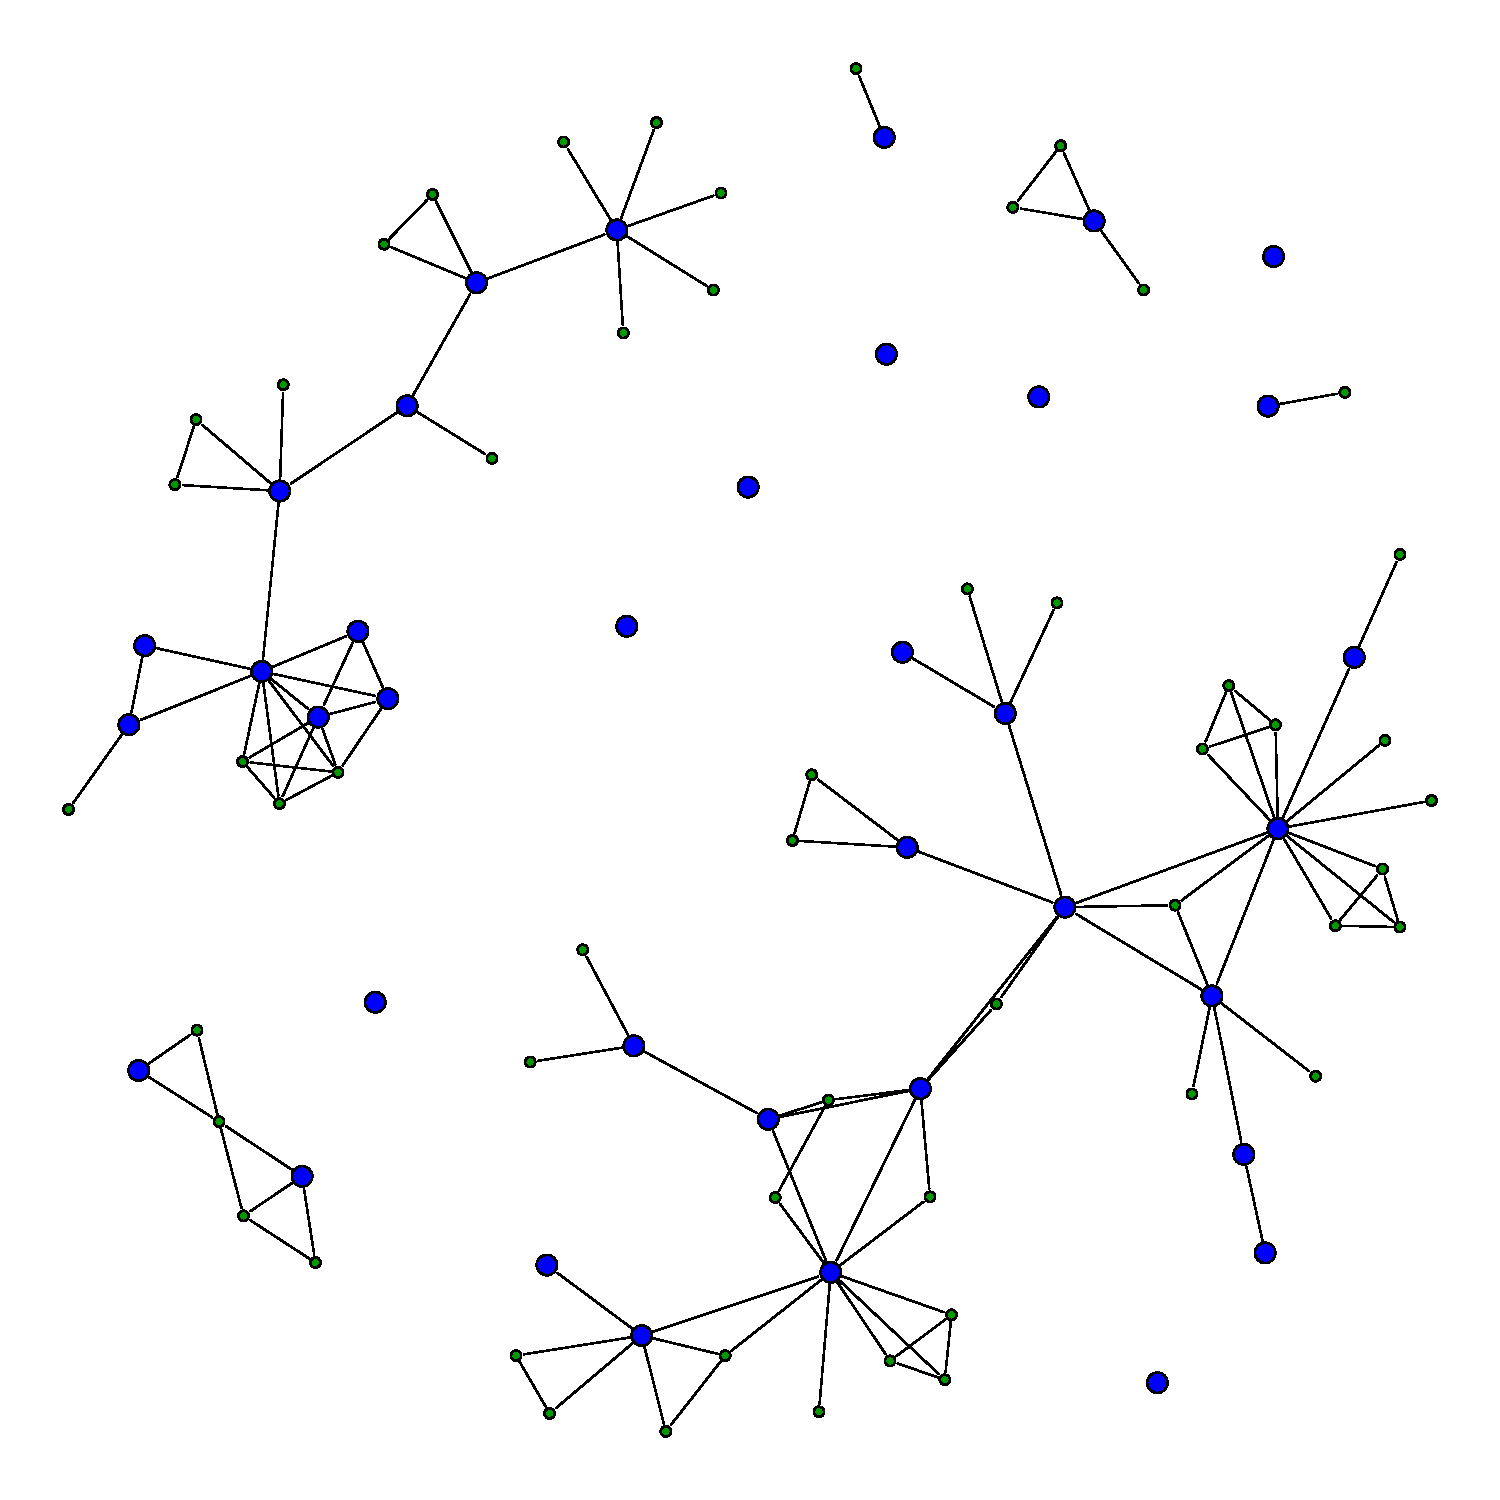
\includegraphics[width=.7\textwidth]{exemplo-grafo}
    \caption{Uma figura simples.\label{fig:subfigures:a}}
  \end{subfigure}
  % ATENÇÃO: Se você deixar uma linha em branco entre as subfiguras,
  % LaTeX vai considerar que cada uma delas pertence a um "parágrafo"
  % diferente e, portanto, vai colocá-las em linhas separadas ao invés
  % de lado a lado.
  \begin{subfigure}{0.4\textwidth}
    \centering
    \begin{turn}{90}
      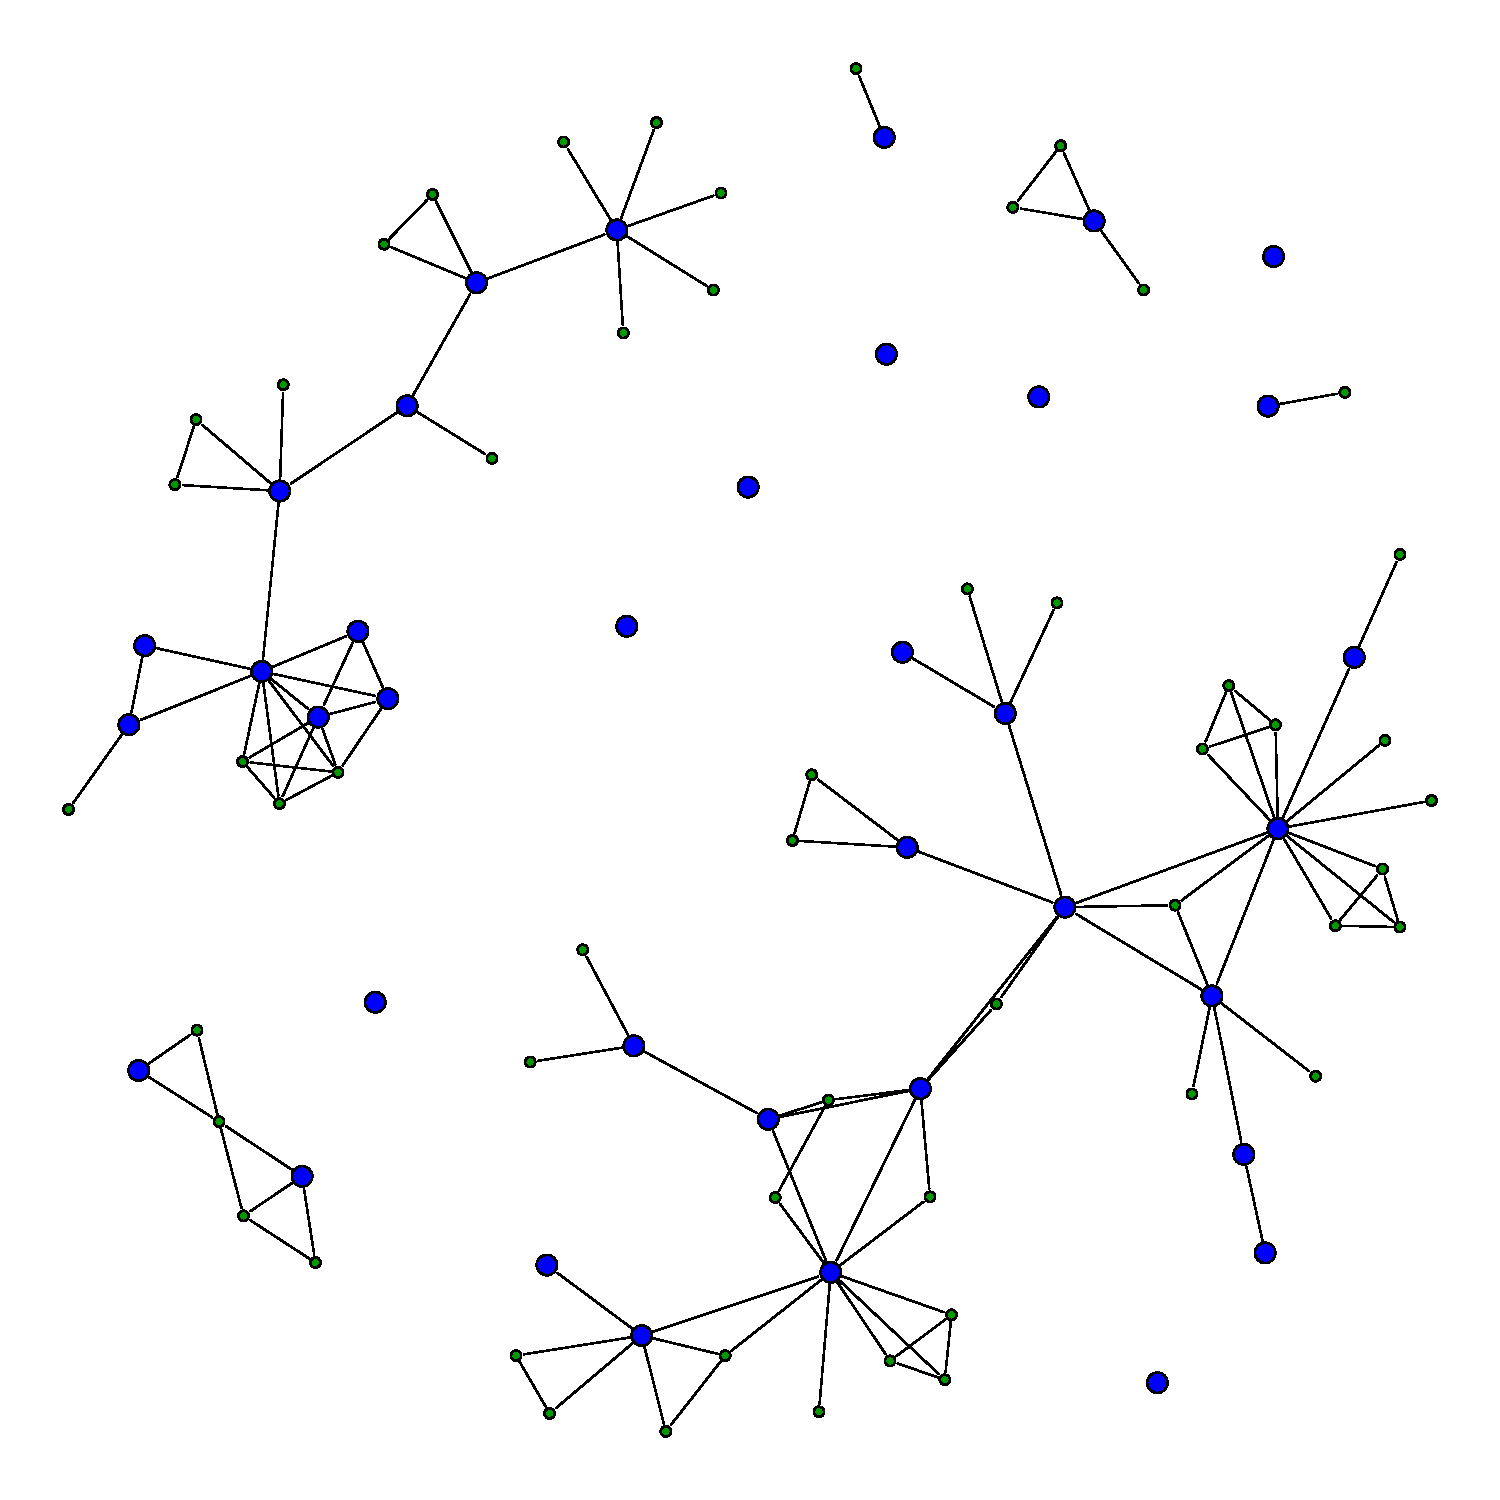
\includegraphics[width=.7\textwidth]{exemplo-grafo}
    \end{turn}
    \caption{O mesmo exemplo, girado.\label{fig:subfigures:b}}
  \end{subfigure}

  \caption{Exemplo de subfiguras.\label{fig:subfigures}}
\end{figure}

Uma ``figura'', na verdade, pode ser qualquer tipo de conteúdo ilustrativo
(um exemplo interessante é o cronograma mostrado na Figura~\ref{fig:gantt}) mas, com a
\textit{package} \textsf{float}, também é possível definir ambientes
específicos para cada tipo de conteúdo adicional (cada um com numeração
independente), como é o caso do Programa~\ref{prog:java}\index{Floats}. Há
mais informações e dicas sobre recursos específicos para inclusão de
código-fonte e pseudocódigo no Apêndice \ref{ap:pseudocode}\footnote{
Observe que o nome do Apêndice (``\ref{ap:pseudocode}'') foi impresso em
uma linha separada, o que não é muito bom visualmente. Para evitar que isso
aconteça (não só no final do parágrafo, mas em qualquer quebra de linha),
faça o que já foi discutido na Seção~\ref{orphanchar} sobre símbolos
matemáticos: utilize um espaço não-separável para fazer referências a
figuras, tabelas, seções etc.: ``\textsf{\dots no
Apêndice\textasciitilde\textbackslash{}ref\{ap:pseudocode\}}''.}.

%%%%%%% Cronograma %%%%%%%

\begin{figure}
  \centering

  \begin{ganttchart}{2017-11}{2018-5}
    \gantttitlecalendar{year,month=shortname} \ganttnewline

    \ganttgroup[progress=45]{Experimento}{2017-11}{2018-2} \ganttnewline
    \ganttbar[progress=100]{
      Preparação\ganttalignnewline
      (compra de insumos)
      }{2017-11}{2017-12} \ganttnewline
    \ganttbar[progress=30]{Execução}{2017-12}{2018-1} \ganttnewline
    \ganttbar[progress=0]{Análise}{2017-12}{2018-2} \ganttnewline

    \ganttgroup[progress=0]{Artigo}{2018-1}{2018-4} \ganttnewline
    \ganttbar[progress=0]{Escrita}{2018-1}{2018-3} \ganttnewline
    \ganttbar[progress=0]{Revisão}{2018-3}{2018-4} \ganttnewline

    \ganttmilestone{Submissão}{2018-4}
  \end{ganttchart}

  \caption{Exemplo de cronograma.\label{fig:gantt}}
\end{figure}

%%%%%%%% Código fonte %%%%%%%%

% Foi utilizado o pacote listings para formatar o código fonte.
% Veja os parâmetros de configuração no arquivo source-code.tex.
\begin{program}
  \index{Java}
  \centering

\begin{lstlisting}[language=Java, style=wider]
  for (i = 0; i < 20; i++)
  {
      // Comentário
      System.out.println("Mensagem...");
  }
\end{lstlisting}

  \caption{Exemplo de laço em Java.\label{prog:java}}
\end{program}

%%%%%

\LaTeX{} pode importar gráficos gerados por \texttt{matplotlib} e por
\texttt{gnuplot} como qualquer outra imagem, mas nesse caso a fonte
usada nesses gráficos provavelmente será diferente do corpo do texto.
Conforme mencionado na Seção~\ref{sec:graficos}, há mecanismos para
resolver esse problema\footnote{Você pode se interessar também pela
package \texttt{gnuplottex}.}, como pode ser visto na
Figura~\ref{fig:graficos}.

\begin{figure}
  \centering
  \begin{subfigure}{.65\textwidth}
    \input{figuras/gnuplot.tkz}
    \caption{\texttt{gnuplot}.\label{fig:gnuplot}}
  \end{subfigure}
  \begin{subfigure}{.3\textwidth}
    %% Creator: Matplotlib, PGF backend
%%
%% To include the figure in your LaTeX document, write
%%   \input{<filename>.pgf}
%%
%% Make sure the required packages are loaded in your preamble
%%   \usepackage{pgf}
%%
%% Figures using additional raster images can only be included by \input if
%% they are in the same directory as the main LaTeX file. For loading figures
%% from other directories you can use the `import` package
%%   \usepackage{import}
%% and then include the figures with
%%   \import{<path to file>}{<filename>.pgf}
%%
%% Matplotlib used the following preamble
%%   \usepackage{fontspec}
%%   \setmainfont{DejaVu Serif}
%%   \setsansfont{DejaVu Sans}
%%   \setmonofont{DejaVu Sans Mono}
%%
\begingroup%
\makeatletter%
\begin{pgfpicture}%
\pgfpathrectangle{\pgfpointorigin}{\pgfqpoint{1.500000in}{2.500000in}}%
\pgfusepath{use as bounding box, clip}%
\begin{pgfscope}%
\pgfsetbuttcap%
\pgfsetmiterjoin%
\definecolor{currentfill}{rgb}{1.000000,1.000000,1.000000}%
\pgfsetfillcolor{currentfill}%
\pgfsetlinewidth{0.000000pt}%
\definecolor{currentstroke}{rgb}{1.000000,1.000000,1.000000}%
\pgfsetstrokecolor{currentstroke}%
\pgfsetdash{}{0pt}%
\pgfpathmoveto{\pgfqpoint{0.000000in}{0.000000in}}%
\pgfpathlineto{\pgfqpoint{1.500000in}{0.000000in}}%
\pgfpathlineto{\pgfqpoint{1.500000in}{2.500000in}}%
\pgfpathlineto{\pgfqpoint{0.000000in}{2.500000in}}%
\pgfpathclose%
\pgfusepath{fill}%
\end{pgfscope}%
\begin{pgfscope}%
\pgfsetbuttcap%
\pgfsetmiterjoin%
\definecolor{currentfill}{rgb}{1.000000,1.000000,1.000000}%
\pgfsetfillcolor{currentfill}%
\pgfsetlinewidth{0.000000pt}%
\definecolor{currentstroke}{rgb}{0.000000,0.000000,0.000000}%
\pgfsetstrokecolor{currentstroke}%
\pgfsetstrokeopacity{0.000000}%
\pgfsetdash{}{0pt}%
\pgfpathmoveto{\pgfqpoint{0.385278in}{0.425278in}}%
\pgfpathlineto{\pgfqpoint{1.452500in}{0.425278in}}%
\pgfpathlineto{\pgfqpoint{1.452500in}{2.437500in}}%
\pgfpathlineto{\pgfqpoint{0.385278in}{2.437500in}}%
\pgfpathclose%
\pgfusepath{fill}%
\end{pgfscope}%
\begin{pgfscope}%
\pgfpathrectangle{\pgfqpoint{0.385278in}{0.425278in}}{\pgfqpoint{1.067222in}{2.012222in}} %
\pgfusepath{clip}%
\pgfsetbuttcap%
\pgfsetmiterjoin%
\definecolor{currentfill}{rgb}{0.121569,0.466667,0.705882}%
\pgfsetfillcolor{currentfill}%
\pgfsetlinewidth{0.000000pt}%
\definecolor{currentstroke}{rgb}{0.000000,0.000000,0.000000}%
\pgfsetstrokecolor{currentstroke}%
\pgfsetstrokeopacity{0.000000}%
\pgfsetdash{}{0pt}%
\pgfpathmoveto{\pgfqpoint{0.385278in}{0.425278in}}%
\pgfpathlineto{\pgfqpoint{0.690198in}{0.425278in}}%
\pgfpathlineto{\pgfqpoint{0.690198in}{1.096019in}}%
\pgfpathlineto{\pgfqpoint{0.385278in}{1.096019in}}%
\pgfpathclose%
\pgfusepath{fill}%
\end{pgfscope}%
\begin{pgfscope}%
\pgfpathrectangle{\pgfqpoint{0.385278in}{0.425278in}}{\pgfqpoint{1.067222in}{2.012222in}} %
\pgfusepath{clip}%
\pgfsetbuttcap%
\pgfsetmiterjoin%
\definecolor{currentfill}{rgb}{0.121569,0.466667,0.705882}%
\pgfsetfillcolor{currentfill}%
\pgfsetlinewidth{0.000000pt}%
\definecolor{currentstroke}{rgb}{0.000000,0.000000,0.000000}%
\pgfsetstrokecolor{currentstroke}%
\pgfsetstrokeopacity{0.000000}%
\pgfsetdash{}{0pt}%
\pgfpathmoveto{\pgfqpoint{0.766429in}{0.425278in}}%
\pgfpathlineto{\pgfqpoint{1.071349in}{0.425278in}}%
\pgfpathlineto{\pgfqpoint{1.071349in}{2.437500in}}%
\pgfpathlineto{\pgfqpoint{0.766429in}{2.437500in}}%
\pgfpathclose%
\pgfusepath{fill}%
\end{pgfscope}%
\begin{pgfscope}%
\pgfpathrectangle{\pgfqpoint{0.385278in}{0.425278in}}{\pgfqpoint{1.067222in}{2.012222in}} %
\pgfusepath{clip}%
\pgfsetbuttcap%
\pgfsetmiterjoin%
\definecolor{currentfill}{rgb}{0.121569,0.466667,0.705882}%
\pgfsetfillcolor{currentfill}%
\pgfsetlinewidth{0.000000pt}%
\definecolor{currentstroke}{rgb}{0.000000,0.000000,0.000000}%
\pgfsetstrokecolor{currentstroke}%
\pgfsetstrokeopacity{0.000000}%
\pgfsetdash{}{0pt}%
\pgfpathmoveto{\pgfqpoint{1.147579in}{0.425278in}}%
\pgfpathlineto{\pgfqpoint{1.452500in}{0.425278in}}%
\pgfpathlineto{\pgfqpoint{1.452500in}{1.766759in}}%
\pgfpathlineto{\pgfqpoint{1.147579in}{1.766759in}}%
\pgfpathclose%
\pgfusepath{fill}%
\end{pgfscope}%
\begin{pgfscope}%
\pgfsetbuttcap%
\pgfsetroundjoin%
\definecolor{currentfill}{rgb}{0.000000,0.000000,0.000000}%
\pgfsetfillcolor{currentfill}%
\pgfsetlinewidth{0.803000pt}%
\definecolor{currentstroke}{rgb}{0.000000,0.000000,0.000000}%
\pgfsetstrokecolor{currentstroke}%
\pgfsetdash{}{0pt}%
\pgfsys@defobject{currentmarker}{\pgfqpoint{0.000000in}{-0.048611in}}{\pgfqpoint{0.000000in}{0.000000in}}{%
\pgfpathmoveto{\pgfqpoint{0.000000in}{0.000000in}}%
\pgfpathlineto{\pgfqpoint{0.000000in}{-0.048611in}}%
\pgfusepath{stroke,fill}%
}%
\begin{pgfscope}%
\pgfsys@transformshift{0.537738in}{0.425278in}%
\pgfsys@useobject{currentmarker}{}%
\end{pgfscope}%
\end{pgfscope}%
\begin{pgfscope}%
\pgftext[x=0.537738in,y=0.328056in,,top]{\rmfamily\fontsize{9.000000}{10.800000}\selectfont SP}%
\end{pgfscope}%
\begin{pgfscope}%
\pgfsetbuttcap%
\pgfsetroundjoin%
\definecolor{currentfill}{rgb}{0.000000,0.000000,0.000000}%
\pgfsetfillcolor{currentfill}%
\pgfsetlinewidth{0.803000pt}%
\definecolor{currentstroke}{rgb}{0.000000,0.000000,0.000000}%
\pgfsetstrokecolor{currentstroke}%
\pgfsetdash{}{0pt}%
\pgfsys@defobject{currentmarker}{\pgfqpoint{0.000000in}{-0.048611in}}{\pgfqpoint{0.000000in}{0.000000in}}{%
\pgfpathmoveto{\pgfqpoint{0.000000in}{0.000000in}}%
\pgfpathlineto{\pgfqpoint{0.000000in}{-0.048611in}}%
\pgfusepath{stroke,fill}%
}%
\begin{pgfscope}%
\pgfsys@transformshift{0.918889in}{0.425278in}%
\pgfsys@useobject{currentmarker}{}%
\end{pgfscope}%
\end{pgfscope}%
\begin{pgfscope}%
\pgftext[x=0.918889in,y=0.328056in,,top]{\rmfamily\fontsize{9.000000}{10.800000}\selectfont RJ}%
\end{pgfscope}%
\begin{pgfscope}%
\pgfsetbuttcap%
\pgfsetroundjoin%
\definecolor{currentfill}{rgb}{0.000000,0.000000,0.000000}%
\pgfsetfillcolor{currentfill}%
\pgfsetlinewidth{0.803000pt}%
\definecolor{currentstroke}{rgb}{0.000000,0.000000,0.000000}%
\pgfsetstrokecolor{currentstroke}%
\pgfsetdash{}{0pt}%
\pgfsys@defobject{currentmarker}{\pgfqpoint{0.000000in}{-0.048611in}}{\pgfqpoint{0.000000in}{0.000000in}}{%
\pgfpathmoveto{\pgfqpoint{0.000000in}{0.000000in}}%
\pgfpathlineto{\pgfqpoint{0.000000in}{-0.048611in}}%
\pgfusepath{stroke,fill}%
}%
\begin{pgfscope}%
\pgfsys@transformshift{1.300040in}{0.425278in}%
\pgfsys@useobject{currentmarker}{}%
\end{pgfscope}%
\end{pgfscope}%
\begin{pgfscope}%
\pgftext[x=1.300040in,y=0.328056in,,top]{\rmfamily\fontsize{9.000000}{10.800000}\selectfont MG}%
\end{pgfscope}%
\begin{pgfscope}%
\pgftext[x=0.918889in,y=0.151528in,,top]{\rmfamily\fontsize{9.000000}{10.800000}\selectfont \textit{Estado}}%
\end{pgfscope}%
\begin{pgfscope}%
\pgfsetbuttcap%
\pgfsetroundjoin%
\definecolor{currentfill}{rgb}{0.000000,0.000000,0.000000}%
\pgfsetfillcolor{currentfill}%
\pgfsetlinewidth{0.803000pt}%
\definecolor{currentstroke}{rgb}{0.000000,0.000000,0.000000}%
\pgfsetstrokecolor{currentstroke}%
\pgfsetdash{}{0pt}%
\pgfsys@defobject{currentmarker}{\pgfqpoint{-0.048611in}{0.000000in}}{\pgfqpoint{0.000000in}{0.000000in}}{%
\pgfpathmoveto{\pgfqpoint{0.000000in}{0.000000in}}%
\pgfpathlineto{\pgfqpoint{-0.048611in}{0.000000in}}%
\pgfusepath{stroke,fill}%
}%
\begin{pgfscope}%
\pgfsys@transformshift{0.385278in}{0.425278in}%
\pgfsys@useobject{currentmarker}{}%
\end{pgfscope}%
\end{pgfscope}%
\begin{pgfscope}%
\pgftext[x=0.208527in,y=0.377792in,left,base]{\rmfamily\fontsize{9.000000}{10.800000}\selectfont 0}%
\end{pgfscope}%
\begin{pgfscope}%
\pgfsetbuttcap%
\pgfsetroundjoin%
\definecolor{currentfill}{rgb}{0.000000,0.000000,0.000000}%
\pgfsetfillcolor{currentfill}%
\pgfsetlinewidth{0.803000pt}%
\definecolor{currentstroke}{rgb}{0.000000,0.000000,0.000000}%
\pgfsetstrokecolor{currentstroke}%
\pgfsetdash{}{0pt}%
\pgfsys@defobject{currentmarker}{\pgfqpoint{-0.048611in}{0.000000in}}{\pgfqpoint{0.000000in}{0.000000in}}{%
\pgfpathmoveto{\pgfqpoint{0.000000in}{0.000000in}}%
\pgfpathlineto{\pgfqpoint{-0.048611in}{0.000000in}}%
\pgfusepath{stroke,fill}%
}%
\begin{pgfscope}%
\pgfsys@transformshift{0.385278in}{0.760648in}%
\pgfsys@useobject{currentmarker}{}%
\end{pgfscope}%
\end{pgfscope}%
\begin{pgfscope}%
\pgftext[x=0.208527in,y=0.713163in,left,base]{\rmfamily\fontsize{9.000000}{10.800000}\selectfont 1}%
\end{pgfscope}%
\begin{pgfscope}%
\pgfsetbuttcap%
\pgfsetroundjoin%
\definecolor{currentfill}{rgb}{0.000000,0.000000,0.000000}%
\pgfsetfillcolor{currentfill}%
\pgfsetlinewidth{0.803000pt}%
\definecolor{currentstroke}{rgb}{0.000000,0.000000,0.000000}%
\pgfsetstrokecolor{currentstroke}%
\pgfsetdash{}{0pt}%
\pgfsys@defobject{currentmarker}{\pgfqpoint{-0.048611in}{0.000000in}}{\pgfqpoint{0.000000in}{0.000000in}}{%
\pgfpathmoveto{\pgfqpoint{0.000000in}{0.000000in}}%
\pgfpathlineto{\pgfqpoint{-0.048611in}{0.000000in}}%
\pgfusepath{stroke,fill}%
}%
\begin{pgfscope}%
\pgfsys@transformshift{0.385278in}{1.096019in}%
\pgfsys@useobject{currentmarker}{}%
\end{pgfscope}%
\end{pgfscope}%
\begin{pgfscope}%
\pgftext[x=0.208527in,y=1.048533in,left,base]{\rmfamily\fontsize{9.000000}{10.800000}\selectfont 2}%
\end{pgfscope}%
\begin{pgfscope}%
\pgfsetbuttcap%
\pgfsetroundjoin%
\definecolor{currentfill}{rgb}{0.000000,0.000000,0.000000}%
\pgfsetfillcolor{currentfill}%
\pgfsetlinewidth{0.803000pt}%
\definecolor{currentstroke}{rgb}{0.000000,0.000000,0.000000}%
\pgfsetstrokecolor{currentstroke}%
\pgfsetdash{}{0pt}%
\pgfsys@defobject{currentmarker}{\pgfqpoint{-0.048611in}{0.000000in}}{\pgfqpoint{0.000000in}{0.000000in}}{%
\pgfpathmoveto{\pgfqpoint{0.000000in}{0.000000in}}%
\pgfpathlineto{\pgfqpoint{-0.048611in}{0.000000in}}%
\pgfusepath{stroke,fill}%
}%
\begin{pgfscope}%
\pgfsys@transformshift{0.385278in}{1.431389in}%
\pgfsys@useobject{currentmarker}{}%
\end{pgfscope}%
\end{pgfscope}%
\begin{pgfscope}%
\pgftext[x=0.208527in,y=1.383904in,left,base]{\rmfamily\fontsize{9.000000}{10.800000}\selectfont 3}%
\end{pgfscope}%
\begin{pgfscope}%
\pgfsetbuttcap%
\pgfsetroundjoin%
\definecolor{currentfill}{rgb}{0.000000,0.000000,0.000000}%
\pgfsetfillcolor{currentfill}%
\pgfsetlinewidth{0.803000pt}%
\definecolor{currentstroke}{rgb}{0.000000,0.000000,0.000000}%
\pgfsetstrokecolor{currentstroke}%
\pgfsetdash{}{0pt}%
\pgfsys@defobject{currentmarker}{\pgfqpoint{-0.048611in}{0.000000in}}{\pgfqpoint{0.000000in}{0.000000in}}{%
\pgfpathmoveto{\pgfqpoint{0.000000in}{0.000000in}}%
\pgfpathlineto{\pgfqpoint{-0.048611in}{0.000000in}}%
\pgfusepath{stroke,fill}%
}%
\begin{pgfscope}%
\pgfsys@transformshift{0.385278in}{1.766759in}%
\pgfsys@useobject{currentmarker}{}%
\end{pgfscope}%
\end{pgfscope}%
\begin{pgfscope}%
\pgftext[x=0.208527in,y=1.719274in,left,base]{\rmfamily\fontsize{9.000000}{10.800000}\selectfont 4}%
\end{pgfscope}%
\begin{pgfscope}%
\pgfsetbuttcap%
\pgfsetroundjoin%
\definecolor{currentfill}{rgb}{0.000000,0.000000,0.000000}%
\pgfsetfillcolor{currentfill}%
\pgfsetlinewidth{0.803000pt}%
\definecolor{currentstroke}{rgb}{0.000000,0.000000,0.000000}%
\pgfsetstrokecolor{currentstroke}%
\pgfsetdash{}{0pt}%
\pgfsys@defobject{currentmarker}{\pgfqpoint{-0.048611in}{0.000000in}}{\pgfqpoint{0.000000in}{0.000000in}}{%
\pgfpathmoveto{\pgfqpoint{0.000000in}{0.000000in}}%
\pgfpathlineto{\pgfqpoint{-0.048611in}{0.000000in}}%
\pgfusepath{stroke,fill}%
}%
\begin{pgfscope}%
\pgfsys@transformshift{0.385278in}{2.102130in}%
\pgfsys@useobject{currentmarker}{}%
\end{pgfscope}%
\end{pgfscope}%
\begin{pgfscope}%
\pgftext[x=0.208527in,y=2.054644in,left,base]{\rmfamily\fontsize{9.000000}{10.800000}\selectfont 5}%
\end{pgfscope}%
\begin{pgfscope}%
\pgfsetbuttcap%
\pgfsetroundjoin%
\definecolor{currentfill}{rgb}{0.000000,0.000000,0.000000}%
\pgfsetfillcolor{currentfill}%
\pgfsetlinewidth{0.803000pt}%
\definecolor{currentstroke}{rgb}{0.000000,0.000000,0.000000}%
\pgfsetstrokecolor{currentstroke}%
\pgfsetdash{}{0pt}%
\pgfsys@defobject{currentmarker}{\pgfqpoint{-0.048611in}{0.000000in}}{\pgfqpoint{0.000000in}{0.000000in}}{%
\pgfpathmoveto{\pgfqpoint{0.000000in}{0.000000in}}%
\pgfpathlineto{\pgfqpoint{-0.048611in}{0.000000in}}%
\pgfusepath{stroke,fill}%
}%
\begin{pgfscope}%
\pgfsys@transformshift{0.385278in}{2.437500in}%
\pgfsys@useobject{currentmarker}{}%
\end{pgfscope}%
\end{pgfscope}%
\begin{pgfscope}%
\pgftext[x=0.208527in,y=2.390015in,left,base]{\rmfamily\fontsize{9.000000}{10.800000}\selectfont 6}%
\end{pgfscope}%
\begin{pgfscope}%
\pgftext[x=0.152971in,y=1.431389in,,bottom,rotate=90.000000]{\rmfamily\fontsize{9.000000}{10.800000}\selectfont \(\displaystyle \mu\)}%
\end{pgfscope}%
\begin{pgfscope}%
\pgfsetrectcap%
\pgfsetmiterjoin%
\pgfsetlinewidth{0.803000pt}%
\definecolor{currentstroke}{rgb}{0.000000,0.000000,0.000000}%
\pgfsetstrokecolor{currentstroke}%
\pgfsetdash{}{0pt}%
\pgfpathmoveto{\pgfqpoint{0.385278in}{0.425278in}}%
\pgfpathlineto{\pgfqpoint{0.385278in}{2.437500in}}%
\pgfusepath{stroke}%
\end{pgfscope}%
\begin{pgfscope}%
\pgfsetrectcap%
\pgfsetmiterjoin%
\pgfsetlinewidth{0.803000pt}%
\definecolor{currentstroke}{rgb}{0.000000,0.000000,0.000000}%
\pgfsetstrokecolor{currentstroke}%
\pgfsetdash{}{0pt}%
\pgfpathmoveto{\pgfqpoint{1.452500in}{0.425278in}}%
\pgfpathlineto{\pgfqpoint{1.452500in}{2.437500in}}%
\pgfusepath{stroke}%
\end{pgfscope}%
\begin{pgfscope}%
\pgfsetrectcap%
\pgfsetmiterjoin%
\pgfsetlinewidth{0.803000pt}%
\definecolor{currentstroke}{rgb}{0.000000,0.000000,0.000000}%
\pgfsetstrokecolor{currentstroke}%
\pgfsetdash{}{0pt}%
\pgfpathmoveto{\pgfqpoint{0.385278in}{0.425278in}}%
\pgfpathlineto{\pgfqpoint{1.452500in}{0.425278in}}%
\pgfusepath{stroke}%
\end{pgfscope}%
\begin{pgfscope}%
\pgfsetrectcap%
\pgfsetmiterjoin%
\pgfsetlinewidth{0.803000pt}%
\definecolor{currentstroke}{rgb}{0.000000,0.000000,0.000000}%
\pgfsetstrokecolor{currentstroke}%
\pgfsetdash{}{0pt}%
\pgfpathmoveto{\pgfqpoint{0.385278in}{2.437500in}}%
\pgfpathlineto{\pgfqpoint{1.452500in}{2.437500in}}%
\pgfusepath{stroke}%
\end{pgfscope}%
\end{pgfpicture}%
\makeatother%
\endgroup%

    \caption{\texttt{matplotlib}.\label{fig:matplotlib}}
  \end{subfigure}
	\caption{Exemplos de gráficos gerados externamente}\label{fig:graficos}
\end{figure}

Finalmente, talvez você precise organizar a apresentação da informação na forma de
tabelas\index{Floats}\footnote{Para defini-las com \LaTeX{}, pode valer a pena usar o
sítio \url{www.tablesgenerator.com}.}; Um exemplo simples é a Tabela~\ref{tab:amino_acidos}.

%%%%%%%% Tabelas lado-a-lado %%%%%%%%

\begin{table}
\centering

  \hspace*{\fill}
  \begin{subtable}[b]{0.42\textwidth}
    % \rowcolors é definida pela package xcolor;
    % veja também os recursos da package colortbl
    \rowcolors{2}{lightgray!70}{white}
    \centering
    \begin{tabular}{ccl}
      \toprule
      Código      & Abreviatura  & \makecell{Nome\\completo} \\
      \midrule
      \texttt{A}  & Ala          & Alanina \\
      \texttt{C}  & Cys          & Cisteína \\
      ...         & ...          & ... \\
      \texttt{W}  & Trp          & Triptofano \\
      \texttt{Y}  & Tyr          & Tirosina \\
      \bottomrule
    \end{tabular}
    \caption{Com linhas de cores alternadas.}
  \end{subtable}
  % Como mencionado mais acima, não deixe linhas em branco aqui
  \hspace*{\fill}\hspace*{\fill}\hspace*{\fill}
  \begin{subtable}[b]{0.37\textwidth}
    \centering
    \begin{tabular}{ccl}
      \rothead{Código} & \rothead{Abreviatura} & \rothead{Nome\\completo} \\
      \midrule
      \texttt{A}       & Ala                   & Alanina \\
      \texttt{C}       & Cys                   & Cisteína \\
      ...              & ...                   & ... \\
      \texttt{W}       & Trp                   & Triptofano \\
      \texttt{Y}       & Tyr                   & Tirosina \\
      \bottomrule
    \end{tabular}
    \caption{Com cabeçalhos girados.}
  \end{subtable}
  \hspace*{\fill}

  \caption{Exemplos de tabelas (códigos, abreviaturas e nomes dos aminoácidos).\label{tab:amino_acidos}}
\end{table}

Se a tabela tem muitas linhas e, portanto, não cabe em uma única página, é
possível fazê-la continuar ao longo de várias páginas com a \textit{package}
\textsf{longtable}, como é o caso da Tabela~\ref{tab:numeros}. Nesse caso,
a tabela não é um \textit{float} e, portanto, ela aparece de acordo com a
sequência normal do texto. Se, além de muito longa, a tabela for também
muito larga, você pode usar o comando \textsf{landscape} (da
\textit{package} \textsf{pdflscape}) em conjunto com \textsf{longtable}
para imprimi-la em modo paisagem ao longo de várias páginas. A
Tabela~\ref{tab:numeros} tem essa configuração comentada; experimente
des-comentar as linhas correspondentes\footnote{Observe que, nesse caso,
vai sempre haver uma quebra de página no texto para fazer a tabela
começar em uma página em modo paisagem.}.

%%%%%%%% Tabela longa em várias páginas %%%%%%%%

%%%% É possível fazer esta mesma tabela em modo paisagem des-comentando
%%%% esta linha e a correspondente no final da tabela
%\begin{landscape}
\begin{longtable}[c]{|c|c|c|c|c|c|c|c|c|c|c|c|c|}

%%%%%%%%%%%%
% O cabeçalho da tabela na primeira página em que ela aparece.

\hline
% Como a tabela pode se estender por várias páginas, precisamos tomar
% cuidado especial com \caption e \label: se esses comandos forem
% executados mais de uma vez, a lista de tabelas e as referências à
% tabela ficarão incorretas. Há diversas soluções, mas a mais simples
% é usar "\caption[]", que não coloca a tabela na lista de tabelas, e
% incluí-la manualmente na lista apenas uma vez aqui junto com o \label.
\captionlistentry{Exemplo de tabela com valores numéricos.}\label{tab:numeros}

\emph{Lim.} &
\multicolumn{3}{c|}{MGWT} &
\multicolumn{3}{c|}{AMI} &
\multicolumn{3}{c|}{\emph{Spectrum} de Fourier} &
\multicolumn{3}{c|}{Caract. espectrais} \\

\cline{2-4} \cline{5-7} \cline{8-10} \cline{11-13} &
\emph{Sn} & \emph{Sp} & \emph{AC} &
\emph{Sn} & \emph{Sp} & \emph{AC} &
\emph{Sn} & \emph{Sp} & \emph{AC} &
\emph{Sn} & \emph{Sp} & \emph{AC} \\

\hline \hline

\endfirsthead % Final do cabeçalho que aparece na primeira página

%%%%%%%%%%%%
% O cabeçalho da tabela em todas as páginas em que ela aparece
% exceto a primeira; aqui, igual ao anterior

\hline

\emph{Lim.} &
\multicolumn{3}{c|}{MGWT} &
\multicolumn{3}{c|}{AMI} &
\multicolumn{3}{c|}{\emph{Spectrum} de Fourier} &
\multicolumn{3}{c|}{Caract. espectrais} \\

\cline{2-4} \cline{5-7} \cline{8-10} \cline{11-13} &
\emph{Sn} & \emph{Sp} & \emph{AC} &
\emph{Sn} & \emph{Sp} & \emph{AC} &
\emph{Sn} & \emph{Sp} & \emph{AC} &
\emph{Sn} & \emph{Sp} & \emph{AC} \\

\hline \hline

\endhead % Final do cabeçalho das páginas seguintes à primeira

%%%%%%%%%%%%
% O rodapé da tabela em todas as páginas em que ela aparece
% exceto a última

\hline

\multicolumn{13}{|r|}{\textit{continua}\enspace$\longrightarrow$}\\

\hline

% Como usamos \captionlistentry mais acima, usamos "[]" aqui.
\caption[]{Exemplo de tabela com valores numéricos.}

\endfoot % Final do rodapé que aparece em todas as páginas exceto a última

%%%%%%%%%%%%
% O rodapé da tabela na última página em que ela aparece

\hline

% Como usamos \captionlistentry mais acima, usamos "[]" aqui.
\caption[]{Exemplo de tabela com valores numéricos.}

\endlastfoot % Final do rodapé da última página

%%%%%%%%%%%%
% O conteúdo da tabela de fato.

 1 & 1.00 & 0.16 & 0.08 & 1.00 & 0.16 & 0.08 & 1.00 & 0.16 & 0.08 & 1.00 & 0.16 & 0.08 \\
 2 & 1.00 & 0.16 & 0.09 & 1.00 & 0.16 & 0.09 & 1.00 & 0.16 & 0.09 & 1.00 & 0.16 & 0.09 \\
 3 & 1.00 & 0.16 & 0.10 & 1.00 & 0.16 & 0.10 & 1.00 & 0.16 & 0.10 & 1.00 & 0.16 & 0.10 \\
 4 & 1.00 & 0.16 & 0.10 & 1.00 & 0.16 & 0.10 & 1.00 & 0.16 & 0.10 & 1.00 & 0.16 & 0.10 \\
 5 & 1.00 & 0.16 & 0.11 & 1.00 & 0.16 & 0.11 & 1.00 & 0.16 & 0.11 & 1.00 & 0.16 & 0.11 \\
 6 & 1.00 & 0.16 & 0.12 & 1.00 & 0.16 & 0.12 & 1.00 & 0.16 & 0.12 & 1.00 & 0.16 & 0.12 \\
 7 & 1.00 & 0.17 & 0.12 & 1.00 & 0.17 & 0.12 & 1.00 & 0.17 & 0.12 & 1.00 & 0.17 & 0.13 \\
 8 & 1.00 & 0.17 & 0.13 & 1.00 & 0.17 & 0.13 & 1.00 & 0.17 & 0.13 & 1.00 & 0.17 & 0.13 \\
 9 & 1.00 & 0.17 & 0.14 & 1.00 & 0.17 & 0.14 & 1.00 & 0.17 & 0.14 & 1.00 & 0.17 & 0.14 \\
10 & 1.00 & 0.17 & 0.15 & 1.00 & 0.17 & 0.15 & 1.00 & 0.17 & 0.15 & 1.00 & 0.17 & 0.15 \\
11 & 1.00 & 0.17 & 0.15 & 1.00 & 0.17 & 0.15 & 1.00 & 0.17 & 0.15 & 1.00 & 0.17 & 0.15 \\
12 & 1.00 & 0.18 & 0.16 & 1.00 & 0.18 & 0.16 & 1.00 & 0.18 & 0.16 & 1.00 & 0.18 & 0.16 \\
13 & 1.00 & 0.18 & 0.17 & 1.00 & 0.18 & 0.17 & 1.00 & 0.18 & 0.17 & 1.00 & 0.18 & 0.17 \\
14 & 1.00 & 0.18 & 0.17 & 1.00 & 0.18 & 0.17 & 1.00 & 0.18 & 0.17 & 1.00 & 0.18 & 0.17 \\
% Como nesta página há uma nota de rodapé, a linha separadora da
% nota e o final da tabela ficam muito próximos; vamos forçar uma
% quebra de página uma linha antes para resolver isso.
\pagebreak
15 & 1.00 & 0.18 & 0.18 & 1.00 & 0.18 & 0.18 & 1.00 & 0.18 & 0.18 & 1.00 & 0.18 & 0.18 \\
16 & 1.00 & 0.18 & 0.19 & 1.00 & 0.18 & 0.19 & 1.00 & 0.18 & 0.19 & 1.00 & 0.18 & 0.19 \\
17 & 1.00 & 0.19 & 0.19 & 1.00 & 0.19 & 0.19 & 1.00 & 0.19 & 0.19 & 1.00 & 0.19 & 0.19 \\
18 & 1.00 & 0.19 & 0.20 & 1.00 & 0.19 & 0.20 & 1.00 & 0.19 & 0.20 & 1.00 & 0.19 & 0.20 \\
19 & 1.00 & 0.19 & 0.21 & 1.00 & 0.19 & 0.21 & 1.00 & 0.19 & 0.21 & 1.00 & 0.19 & 0.21 \\
20 & 1.00 & 0.19 & 0.22 & 1.00 & 0.19 & 0.22 & 1.00 & 0.19 & 0.22 & 1.00 & 0.19 & 0.22 \\
21 & 1.00 & 0.19 & 0.22 & 1.00 & 0.19 & 0.22 & 1.00 & 0.19 & 0.22 & 1.00 & 0.19 & 0.22 \\
22 & 1.00 & 0.19 & 0.22 & 1.00 & 0.19 & 0.22 & 1.00 & 0.19 & 0.22 & 1.00 & 0.19 & 0.22 \\
23 & 1.00 & 0.19 & 0.22 & 1.00 & 0.19 & 0.22 & 1.00 & 0.19 & 0.22 & 1.00 & 0.19 & 0.22 \\
24 & 1.00 & 0.19 & 0.22 & 1.00 & 0.19 & 0.22 & 1.00 & 0.19 & 0.22 & 1.00 & 0.19 & 0.22 \\
25 & 1.00 & 0.19 & 0.22 & 1.00 & 0.19 & 0.22 & 1.00 & 0.19 & 0.22 & 1.00 & 0.19 & 0.22 \\
26 & 1.00 & 0.19 & 0.22 & 1.00 & 0.19 & 0.22 & 1.00 & 0.19 & 0.22 & 1.00 & 0.19 & 0.22 \\
27 & 1.00 & 0.19 & 0.22 & 1.00 & 0.19 & 0.22 & 1.00 & 0.19 & 0.22 & 1.00 & 0.19 & 0.22 \\
28 & 1.00 & 0.19 & 0.22 & 1.00 & 0.19 & 0.22 & 1.00 & 0.19 & 0.22 & 1.00 & 0.19 & 0.22 \\
29 & 1.00 & 0.19 & 0.22 & 1.00 & 0.19 & 0.22 & 1.00 & 0.19 & 0.22 & 1.00 & 0.19 & 0.22 \\
30 & 1.00 & 0.19 & 0.22 & 1.00 & 0.19 & 0.22 & 1.00 & 0.19 & 0.22 & 1.00 & 0.19 & 0.22 \\
31 & 1.00 & 0.19 & 0.22 & 1.00 & 0.19 & 0.22 & 1.00 & 0.19 & 0.22 & 1.00 & 0.19 & 0.22 \\
32 & 1.00 & 0.19 & 0.22 & 1.00 & 0.19 & 0.22 & 1.00 & 0.19 & 0.22 & 1.00 & 0.19 & 0.22 \\
33 & 1.00 & 0.19 & 0.22 & 1.00 & 0.19 & 0.22 & 1.00 & 0.19 & 0.22 & 1.00 & 0.19 & 0.22 \\
34 & 1.00 & 0.19 & 0.22 & 1.00 & 0.19 & 0.22 & 1.00 & 0.19 & 0.22 & 1.00 & 0.19 & 0.22 \\
35 & 1.00 & 0.19 & 0.22 & 1.00 & 0.19 & 0.22 & 1.00 & 0.19 & 0.22 & 1.00 & 0.19 & 0.22 \\
36 & 1.00 & 0.19 & 0.22 & 1.00 & 0.19 & 0.22 & 1.00 & 0.19 & 0.22 & 1.00 & 0.19 & 0.22 \\
37 & 1.00 & 0.19 & 0.22 & 1.00 & 0.19 & 0.22 & 1.00 & 0.19 & 0.22 & 1.00 & 0.19 & 0.22 \\
38 & 1.00 & 0.19 & 0.22 & 1.00 & 0.19 & 0.22 & 1.00 & 0.19 & 0.22 & 1.00 & 0.19 & 0.22 \\
39 & 1.00 & 0.19 & 0.22 & 1.00 & 0.19 & 0.22 & 1.00 & 0.19 & 0.22 & 1.00 & 0.19 & 0.22 \\
40 & 1.00 & 0.19 & 0.22 & 1.00 & 0.19 & 0.22 & 1.00 & 0.19 & 0.22 & 1.00 & 0.19 & 0.22 \\
\end{longtable}
%\end{landscape}

Tabelas mais complexas são um tanto trabalhosas em \LaTeX{}; a
Tabela~\ref{tab:ficha} mostra como construir uma tabela em forma de ficha.
Além de complexa, ela é larga e, portanto, deve ser impressa em modo
paisagem. No entanto, usamos um outro mecanismo para girar a tabela: o
comando \textsf{sidewaystable} (da \textit{package} \textsf{rotating}).
Com esse mecanismo, ela continua sendo um \textit{float} (e, portanto,
não força quebras de página no meio do texto), mas sempre é impressa em
uma página separada.

Resumindo:

\begin{itemize}
  \item Se uma tabela cabe em uma página, defina-a como um \textit{float};
  \item se cabe em uma página mas é muito larga e precisa ser impressa em
        modo paisagem, use \textsf{sidewaystable} (que também é um \textit{float});
  \item se não cabe em uma página por ser muito longa, use \textsf{longtable};
  \item se não cabe em uma página por ser muito longa e precisa ser impressa
        em modo paisagem por ser muito larga, use \textsf{longtable} em
        conjunto com \textsf{landscape}.
\end{itemize}

%%%%%%%% Tabela em forma de ficha %%%%%%%%

% Aumenta o espaçamento entre as linhas da tabela (default: 0pt)
\setlength\extrarowheight{4pt}

% sidewaystable e comandos relacionados são definidos na package rotating
\begin{sidewaystable}
\centering

\begin{tabular}{|M{0.265}|M{0.073}|M{0.084}|M{0.073}|M{0.073}|M{0.08}|M{0.082}|M{0.067}|}
  \hline
    \textbf{Experimento número:} & \multicolumn{2}{c|}{1} & \multicolumn{4}{c|}{\textbf{Data:}} & jan 2017
  \tabularnewline \hline
    \textbf{Título:} & \multicolumn{7}{c|}{Medições iniciais}
  \tabularnewline \hline
    \textbf{Tipo de experimento:} & \multicolumn{7}{c|}{Levantamento quantitativo}
  \tabularnewline \hline \hline
    \textbf{Locais}          & São Paulo & Rio de Janeiro & Porto Alegre & Recife & Manaus & Brasília & Rio Branco
  \tabularnewline \thickhline
    \textbf{Valores obtidos} & 0.2       & 0.3            & 0.2          & 0.7    & 0.5    & 0.1      & 0.4
  \tabularnewline \hline
\end{tabular}

\caption{Exemplo de tabela similar a uma ficha.\label{tab:ficha}}
\end{sidewaystable}

% Redefinindo para o valor default
\setlength\extrarowheight{0pt}

\par

\par


%%%%%%%%%%%%%%%%%%%%%%%%%%%% APÊNDICES E ANEXOS %%%%%%%%%%%%%%%%%%%%%%%%%%%%%%%%

% Um apêndice é algum conteúdo adicional de sua autoria que colabora com a
% ideia geral do texto mas que, por alguma razão, não precisa fazer parte
% da sequência do discurso; por exemplo, a demonstração de um teorema, as
% perguntas usadas em uma pesquisa qualitativa etc.
%
% Um anexo é um documento que não é de sua autoria mas que é relevante para
% a tese; por exemplo, a especificação do padrão que o trabalho discute.
%
% Os comandos appendix e annex reiniciam a numeração de capítulos e passam
% a numerá-los com letras. "annex" não faz parte de nenhuma classe padrão,
% ele foi criado para este modelo (em annex.sty e utils.tex). Se o
% trabalho não tiver apêndices ou anexos, remova estas linhas.
%
% Diferentemente de \mainmatter, \backmatter etc., \appendix e \annex não
% forçam o início de uma nova página. Em geral isso não é importante, pois
% o comando seguinte costuma ser "\chapter", mas pode causar problemas com
% a formatação dos cabeçalhos. Assim, vamos forçar uma nova página antes
% de cada um deles.

%%%% Apêndices %%%%
\makeatletter
\if@openright\cleardoublepage\else\clearpage\fi
\makeatother

% Este formato está definido na package imeusp-headers.
\pagestyle{appendix}

\appendix

%%!TeX root=../tese.tex
%("dica" para o editor de texto: este arquivo é parte de um documento maior)
% para saber mais: https://tex.stackexchange.com/q/78101/183146

% Os apêndices podem ser inseridos diretamente aqui ou "puxados" de outros
% arquivos.
% Em alguns (raros) casos, pode ser interessante usar \include ao
% invés de \input: https://tex.stackexchange.com/a/32058/183146
%!TeX root=../tese.tex
%("dica" para o editor de texto: este arquivo é parte de um documento maior)
% para saber mais: https://tex.stackexchange.com/q/78101/183146

\chapter{Código-Fonte e Pseudocódigo}
\label{ap:pseudocode}

Com a \textit{package} \textsf{listings}, programas podem ser inseridos
diretamente no arquivo, como feito no caso do Programa~\ref{prog:java},
ou importados de um arquivo externo com o comando
\textsf{\textbackslash{}lstinputlisting}, como no caso
do Programa~\ref{prog:mdcinput}.

% O exemplo foi copiado da documentação de algorithmicx
\begin{program}
  \lstinputlisting[
    language=pseudocode,
    style=pseudocode,
    style=wider,
    functions={},
    specialidentifiers={},
  ]
  {conteudo-exemplo/euclid.psc}

  \caption{Máximo divisor comum (arquivo importado).\label{prog:mdcinput}}
\end{program}

Trechos de código curtos (menores que uma página) podem ou não ser
incluídos como \textit{floats}; trechos longos necessariamente incluem
quebras de página e, portanto, não podem ser \textit{floats}. Com
\textit{floats}, a legenda e as linhas separadoras são colocadas pelo
comando \textsf{\textbackslash{}begin\{program\}}; sem eles, utilize o
ambiente \textsf{programruledcaption} (atenção para a colocação do
comando \textsf{\textbackslash{}label\{\}}, dentro da legenda), como
no Programa~\ref{prog:mdc}\footnote{\textsf{listings} oferece alguns
recursos próprios para a definição de \textit{floats} e legendas, mas
neste modelo não os utilizamos.}:

\begin{programruledcaption}{Máximo divisor comum.\label{prog:mdc}}
  \begin{lstlisting}[
    language=pseudocode,
    style=pseudocode,
    style=wider,
    functions={},
    specialidentifiers={},
  ]
      function euclid(a, b) // The \textbf{g.c.d.} of a and b
          r := a $\bmod$ b
          while r != 0 // We have the answer if r is 0
              a := b
              b := r
              r := a $\bmod$ b
          end
          return b // The \textbf{g.c.d.} is b
      end
  \end{lstlisting}
\end{programruledcaption}

Além do suporte às várias linguagens incluídas em \textsf{listings},
este modelo traz uma extensão para permitir o uso de pseudocódigo,
útil para a descrição de algoritmos em alto nível. Ela oferece
diversos recursos:

\begin{itemize}

    \item Comentários seguem o padrão de C++ (\lstinline{//} e
          \lstinline{/* ... */}), mas o delimitador é impresso
          como ``$\triangleright$''.

    \item ``:='', ``<>'', ``<='', ``>='' e ``!='' são substituídos
          pelo símbolo matemático adequado.

    \item É possível acrescentar palavras-chave além de ``if'', ``and''
          etc. com a opção ``\textsf{morekeywords=\{pchave1,\linebreak[0]{}pchave2\}}''
          (para um trecho de código específico) ou com o comando
          \textsf{\textbackslash{}lstset\{morekeywords=\linebreak[0]{}\{pchave1,pchave2\}\}}
          (como comando de configuração geral).

    \item É possível usar pequenos trechos de código, como nomes de variáveis,
          dentro de um parágrafo normal com \textsf{\textbackslash{}lstinline\{blah\}}.

    \item ``\$\dots\$'' ativa o modo matemático em qualquer lugar.

    \item Outros comandos LaTeX funcionam apenas em comentários; fora, a
          linguagem simula alguns pré-definidos (\textsf{\textbackslash{}textit\{\}},
          \textsf{\textbackslash{}texttt\{\}} etc.).

    \item O comando \textsf{\textbackslash{}label} também funciona em
          comentários; a referência correspondente (\textsf{\textbackslash{}ref})
          indica o número da linha de código. Se quiser usá-lo numa linha sem
          comentários, use \lstinline{///}~\textsf{\textbackslash{}label\{blah\}};
          ``\lstinline{///}'' funciona como \lstinline{//}, permitindo
          a inserção de comandos \LaTeX{}, mas não imprime o delimitador
          (\ensuremath{\triangleright}).

    \item Para suspender a formatação automática, use \textsf{\textbackslash{}noparse\{blah\}}.

    \item Para forçar a formatação de um texto como função, identificador,
          palavra-chave ou comentário, use \textsf{\textbackslash{}func\{blah\}},
          \textsf{\textbackslash{}id\{blah\}}, \textsf{\textbackslash{}kw\{blah\}} ou
          \textsf{\textbackslash{}comment\{blah\}}.

    \item Palavras-chave dentro de comentários não são formatadas
          automaticamente; se necessário, use \textsf{\textbackslash{}func\{\}},
          \textsf{\textbackslash{}id\{\}} etc. ou comandos \LaTeX{} padrão.

    \item As palavras ``Program'', ``Procedure'' e ``Function'' têm formatação
          especial e fazem a palavra seguinte ser formatada como função.
          Funções em outros lugares \emph{não} são detectadas automaticamente;
          use \textsf{\textbackslash{}func\{\}}, a opção ``\textsf{functions=\{func1,func2\}}''
          ou o comando ``\textsf{\textbackslash{}lstset\{functions=\{func1,func2\}\}}''
          para que elas sejam detectadas.

    \item Além de funções, palavras-chave, strings, comentários e
          identificadores, há ``\textsf{specialidentifiers}''. Você pode
          usá-los com \textsf{\textbackslash{}specialid\{blah\}}, com a opção
          ``\textsf{specialidentifiers=\{id1,id2\}}'' ou com o comando
          ``\textsf{\textbackslash{}lstset\{specialidentifiers=\{id1,id2\}\}}''.

\end{itemize}



\par

%!TeX root=../tese.tex
%("dica" para o editor de texto: este arquivo é parte de um documento maior)
% para saber mais: https://tex.stackexchange.com/q/78101/183146

% Os apêndices podem ser inseridos diretamente aqui ou "puxados" de outros
% arquivos.
% Em alguns (raros) casos, pode ser interessante usar \include ao
% invés de \input: https://tex.stackexchange.com/a/32058/183146
%!TeX root=../tese.tex
%("dica" para o editor de texto: este arquivo é parte de um documento maior)
% para saber mais: https://tex.stackexchange.com/q/78101/183146

\chapter{Código-Fonte e Pseudocódigo}
\label{ap:pseudocode}

Com a \textit{package} \textsf{listings}, programas podem ser inseridos
diretamente no arquivo, como feito no caso do Programa~\ref{prog:java},
ou importados de um arquivo externo com o comando
\textsf{\textbackslash{}lstinputlisting}, como no caso
do Programa~\ref{prog:mdcinput}.

% O exemplo foi copiado da documentação de algorithmicx
\begin{program}
  \lstinputlisting[
    language=pseudocode,
    style=pseudocode,
    style=wider,
    functions={},
    specialidentifiers={},
  ]
  {conteudo-exemplo/euclid.psc}

  \caption{Máximo divisor comum (arquivo importado).\label{prog:mdcinput}}
\end{program}

Trechos de código curtos (menores que uma página) podem ou não ser
incluídos como \textit{floats}; trechos longos necessariamente incluem
quebras de página e, portanto, não podem ser \textit{floats}. Com
\textit{floats}, a legenda e as linhas separadoras são colocadas pelo
comando \textsf{\textbackslash{}begin\{program\}}; sem eles, utilize o
ambiente \textsf{programruledcaption} (atenção para a colocação do
comando \textsf{\textbackslash{}label\{\}}, dentro da legenda), como
no Programa~\ref{prog:mdc}\footnote{\textsf{listings} oferece alguns
recursos próprios para a definição de \textit{floats} e legendas, mas
neste modelo não os utilizamos.}:

\begin{programruledcaption}{Máximo divisor comum.\label{prog:mdc}}
  \begin{lstlisting}[
    language=pseudocode,
    style=pseudocode,
    style=wider,
    functions={},
    specialidentifiers={},
  ]
      function euclid(a, b) // The \textbf{g.c.d.} of a and b
          r := a $\bmod$ b
          while r != 0 // We have the answer if r is 0
              a := b
              b := r
              r := a $\bmod$ b
          end
          return b // The \textbf{g.c.d.} is b
      end
  \end{lstlisting}
\end{programruledcaption}

Além do suporte às várias linguagens incluídas em \textsf{listings},
este modelo traz uma extensão para permitir o uso de pseudocódigo,
útil para a descrição de algoritmos em alto nível. Ela oferece
diversos recursos:

\begin{itemize}

    \item Comentários seguem o padrão de C++ (\lstinline{//} e
          \lstinline{/* ... */}), mas o delimitador é impresso
          como ``$\triangleright$''.

    \item ``:='', ``<>'', ``<='', ``>='' e ``!='' são substituídos
          pelo símbolo matemático adequado.

    \item É possível acrescentar palavras-chave além de ``if'', ``and''
          etc. com a opção ``\textsf{morekeywords=\{pchave1,\linebreak[0]{}pchave2\}}''
          (para um trecho de código específico) ou com o comando
          \textsf{\textbackslash{}lstset\{morekeywords=\linebreak[0]{}\{pchave1,pchave2\}\}}
          (como comando de configuração geral).

    \item É possível usar pequenos trechos de código, como nomes de variáveis,
          dentro de um parágrafo normal com \textsf{\textbackslash{}lstinline\{blah\}}.

    \item ``\$\dots\$'' ativa o modo matemático em qualquer lugar.

    \item Outros comandos LaTeX funcionam apenas em comentários; fora, a
          linguagem simula alguns pré-definidos (\textsf{\textbackslash{}textit\{\}},
          \textsf{\textbackslash{}texttt\{\}} etc.).

    \item O comando \textsf{\textbackslash{}label} também funciona em
          comentários; a referência correspondente (\textsf{\textbackslash{}ref})
          indica o número da linha de código. Se quiser usá-lo numa linha sem
          comentários, use \lstinline{///}~\textsf{\textbackslash{}label\{blah\}};
          ``\lstinline{///}'' funciona como \lstinline{//}, permitindo
          a inserção de comandos \LaTeX{}, mas não imprime o delimitador
          (\ensuremath{\triangleright}).

    \item Para suspender a formatação automática, use \textsf{\textbackslash{}noparse\{blah\}}.

    \item Para forçar a formatação de um texto como função, identificador,
          palavra-chave ou comentário, use \textsf{\textbackslash{}func\{blah\}},
          \textsf{\textbackslash{}id\{blah\}}, \textsf{\textbackslash{}kw\{blah\}} ou
          \textsf{\textbackslash{}comment\{blah\}}.

    \item Palavras-chave dentro de comentários não são formatadas
          automaticamente; se necessário, use \textsf{\textbackslash{}func\{\}},
          \textsf{\textbackslash{}id\{\}} etc. ou comandos \LaTeX{} padrão.

    \item As palavras ``Program'', ``Procedure'' e ``Function'' têm formatação
          especial e fazem a palavra seguinte ser formatada como função.
          Funções em outros lugares \emph{não} são detectadas automaticamente;
          use \textsf{\textbackslash{}func\{\}}, a opção ``\textsf{functions=\{func1,func2\}}''
          ou o comando ``\textsf{\textbackslash{}lstset\{functions=\{func1,func2\}\}}''
          para que elas sejam detectadas.

    \item Além de funções, palavras-chave, strings, comentários e
          identificadores, há ``\textsf{specialidentifiers}''. Você pode
          usá-los com \textsf{\textbackslash{}specialid\{blah\}}, com a opção
          ``\textsf{specialidentifiers=\{id1,id2\}}'' ou com o comando
          ``\textsf{\textbackslash{}lstset\{specialidentifiers=\{id1,id2\}\}}''.

\end{itemize}



\par

\par

%%%% Anexos %%%%
\makeatletter
\if@openright\cleardoublepage\else\clearpage\fi
\makeatother

% Este formato está definido na package imeusp-headers (note que é o mesmo
% que o anterior; repetimos aqui caso você queira desabilitar toda a seção
% de apêndices).
\pagestyle{appendix}

\annex

%%!TeX root=../tese.tex
%("dica" para o editor de texto: este arquivo é parte de um documento maior)
% para saber mais: https://tex.stackexchange.com/q/78101/183146

% Apague as duas linhas abaixo (elas servem apenas para gerar um
% aviso no arquivo PDF quando não há nenhum dado a imprimir) e
% insira aqui o conteúdo dos anexos do seu trabalho (ou deixe este
% arquivo vazio)

\providecommand\aviso[1]{
  \clearpage
  \null
  \vfill
  \begin{hyphenrules}{nohyphenation}
    \centering\bfseries\Large
    #1\par
  \end{hyphenrules}
  \vfill
  \clearpage
}

\providecommand\avisoFolhasDeRosto{
  \aviso{
    {\huge Você precisa editar os arquivos no diretório ``\texttt{conteudo}''!}
    \par\bigskip\bigskip\bigskip\bigskip
    Para gerar a capa e demais folhas de rosto no formato correto,
    modifique o arquivo ``\texttt{conteudo/folhas-de-rosto.tex}'',
    usando como base o arquivo correspondente no diretório
    ``\texttt{conteudo-exemplo}''.
  }
}

\providecommand\avisoCapitulos{
  \aviso{
    Insira o conteúdo dos capítulos do seu trabalho no arquivo
    ``\texttt{capitulos.tex}'' do diretório ``\texttt{conteudo}''.
  }
}

\providecommand\avisoApendices{
  \aviso{
    Insira o conteúdo dos apêndices do seu trabalho no arquivo
    ``\texttt{apendices.tex}'' do diretório ``\texttt{conteudo}''.
  }
}

\providecommand\avisoAnexos{
  \aviso{
    Insira o conteúdo dos anexos do seu trabalho no arquivo
    ``\texttt{anexos.tex}'' do diretório ``\texttt{conteudo}''.
  }
}

\providecommand\avisoArtigo{
  \aviso{
    Insira o conteúdo do artigo no arquivo ``\texttt{corpo-artigo.tex}''
    do diretório ``\texttt{conteudo}''. Não se esqueça de consultar
    o exemplo no diretório ``\texttt{conteudo-exemplo}'' para a
    definição do título, autoria etc.
  }
}

\providecommand\avisoApresentacao{
  \begin{frame}{Insira o conteúdo!}
  \aviso{
    Insira o conteúdo da apresentação no arquivo ``\texttt{corpo-apresentacao.tex}''
    do diretório ``\texttt{conteudo}''. Não se esqueça de consultar
    o exemplo no diretório ``\texttt{conteudo-exemplo}'' para a
    definição do título, autoria, estrutura etc.
  }
  \end{frame}
}

\providecommand\avisoPoster{
  \begin{document}
  \aviso{
    Insira o conteúdo do poster no arquivo ``\texttt{corpo-poster.tex}''
    do diretório ``\texttt{conteudo}''. Não se esqueça de consultar
    o exemplo no diretório ``\texttt{conteudo-exemplo}'' para a
    definição do título, autoria, estrutura etc.
  }
  \end{document}
}

\providecommand\avisoResumo{
  \aviso{
    Insira o conteúdo do resumo e do abstract no arquivo
    ``\texttt{resumo-abstract.tex}'' do diretório ``\texttt{conteudo}''.
  }
}

\avisoAnexos

% Os anexos podem ser inseridos diretamente aqui ou "puxados" de outros
% arquivos.
% Em alguns (raros) casos, pode ser interessante usar \include ao
% invés de \input: https://tex.stackexchange.com/a/32058/183146

%\input{conteudo/...}
%\par

%!TeX root=../tese.tex
%("dica" para o editor de texto: este arquivo é parte de um documento maior)
% para saber mais: https://tex.stackexchange.com/q/78101/183146

% Apague as duas linhas abaixo (elas servem apenas para gerar um
% aviso no arquivo PDF quando não há nenhum dado a imprimir) e
% insira aqui o conteúdo dos anexos do seu trabalho (ou deixe este
% arquivo vazio)

\providecommand\aviso[1]{
  \clearpage
  \null
  \vfill
  \begin{hyphenrules}{nohyphenation}
    \centering\bfseries\Large
    #1\par
  \end{hyphenrules}
  \vfill
  \clearpage
}

\providecommand\avisoFolhasDeRosto{
  \aviso{
    {\huge Você precisa editar os arquivos no diretório ``\texttt{conteudo}''!}
    \par\bigskip\bigskip\bigskip\bigskip
    Para gerar a capa e demais folhas de rosto no formato correto,
    modifique o arquivo ``\texttt{conteudo/folhas-de-rosto.tex}'',
    usando como base o arquivo correspondente no diretório
    ``\texttt{conteudo-exemplo}''.
  }
}

\providecommand\avisoCapitulos{
  \aviso{
    Insira o conteúdo dos capítulos do seu trabalho no arquivo
    ``\texttt{capitulos.tex}'' do diretório ``\texttt{conteudo}''.
  }
}

\providecommand\avisoApendices{
  \aviso{
    Insira o conteúdo dos apêndices do seu trabalho no arquivo
    ``\texttt{apendices.tex}'' do diretório ``\texttt{conteudo}''.
  }
}

\providecommand\avisoAnexos{
  \aviso{
    Insira o conteúdo dos anexos do seu trabalho no arquivo
    ``\texttt{anexos.tex}'' do diretório ``\texttt{conteudo}''.
  }
}

\providecommand\avisoArtigo{
  \aviso{
    Insira o conteúdo do artigo no arquivo ``\texttt{corpo-artigo.tex}''
    do diretório ``\texttt{conteudo}''. Não se esqueça de consultar
    o exemplo no diretório ``\texttt{conteudo-exemplo}'' para a
    definição do título, autoria etc.
  }
}

\providecommand\avisoApresentacao{
  \begin{frame}{Insira o conteúdo!}
  \aviso{
    Insira o conteúdo da apresentação no arquivo ``\texttt{corpo-apresentacao.tex}''
    do diretório ``\texttt{conteudo}''. Não se esqueça de consultar
    o exemplo no diretório ``\texttt{conteudo-exemplo}'' para a
    definição do título, autoria, estrutura etc.
  }
  \end{frame}
}

\providecommand\avisoPoster{
  \begin{document}
  \aviso{
    Insira o conteúdo do poster no arquivo ``\texttt{corpo-poster.tex}''
    do diretório ``\texttt{conteudo}''. Não se esqueça de consultar
    o exemplo no diretório ``\texttt{conteudo-exemplo}'' para a
    definição do título, autoria, estrutura etc.
  }
  \end{document}
}

\providecommand\avisoResumo{
  \aviso{
    Insira o conteúdo do resumo e do abstract no arquivo
    ``\texttt{resumo-abstract.tex}'' do diretório ``\texttt{conteudo}''.
  }
}

\avisoAnexos

% Os anexos podem ser inseridos diretamente aqui ou "puxados" de outros
% arquivos.
% Em alguns (raros) casos, pode ser interessante usar \include ao
% invés de \input: https://tex.stackexchange.com/a/32058/183146

%\input{conteudo/...}
%\par

\par


%%%%%%%%%%%%%%%%%%%%%%%%%%%%%% SEÇÕES FINAIS %%%%%%%%%%%%%%%%%%%%%%%%%%%%%%%%%%%

% Aqui vão a bibliografia, índice remissivo e outras seções similares.

% O comando backmatter desabilita a numeração de capítulos.
\backmatter

% Este formato está definido na package imeusp-headers
\pagestyle{backmatter}

% Espaço adicional no sumário antes das referências / índice remissivo
\addtocontents{toc}{\vspace{2\baselineskip plus .5\baselineskip minus .5\baselineskip}}

% A bibliografia é obrigatória

%%%%%%%%% Bibliografia com bibtex (preterido): %%%%%%%%%
%\bibliographystyle{extras/alpha-ime}% citação bibliográfica alpha
%\bibliographystyle{extras/plainnat-ime} % citação bibliográfica textual
%\bibliography{bibliografia}  % associado ao arquivo: 'bibliografia.bib'

%%%%%%%% Bibliografia com biblatex (preferido): %%%%%%%%

\printbibliography[
  title=\refname\label{bibliografia}, % "Referências", recomendado pela ABNT
  %title=\bibname\label{bibliografia}, % "Bibliografia"
  % Inclui a bibliografia no sumário
  heading=bibintoc,
]

% imprime o índice remissivo no documento (opcional)
\printindex

\end{document}
